%%%%%%%%%%%%%%%%%%%%%%%%%%%%%%%%%%%%%%%%%%%%%%%%%%%%%%%%%%%%%%%%%%%%%%%%%%%%%%%
%                     Heriot-Watt University Thesis Template  
%   Created by : Lavinia Burski
%   Date:        November 2014
%   Department of Computer Science
%   Heriot-Watt University
%
%%%%%%%%%%%%%%%%%%%%%%%%%%%%%%%%%%%%%%%%%%%%%%%%%%%%%%%%%%%%%%%%%%%%%%%%%%%%%%%

\documentclass[a4paper,12pt]{report}


%==============================title page info=================================

% Name of the author
\newcommand{\auth}{Lavinia Burski}   
% Title of Thesis                
\newcommand{\thesistitle}{From Formal Specification to Full Proof:\newline A Stepwise Method}
% Degree  
\newcommand{\degree}{Doctor of Philosophy} 
% Date submitted
\newcommand{\supdate}{March 2016}            

%===================================packages===================================
\usepackage[top=20mm, bottom=20mm, left=40mm, right=20mm]{geometry}
\usepackage{setspace}
\usepackage{fancyhdr}
\usepackage[citecolor=black, urlcolor=black,
  linkcolor=black, colorlinks=true, bookmarksopen=false, bookmarks=true]{hyperref}
\usepackage[nonumberlist, acronym]{glossaries}
%Glossaries
\makeglossaries

% You must define terms or symbols before you can use them in the document. This is best done in the preamble. Each term is defined using:
% 
% \newglossaryentry{<label>}{<settings>}
% 
% where <label> is a unique label used to identify the term. The second argument, <settings>, is a key=value comma separated list that is used to set the required information for the term. A full list of available keys can be found in "Defining Glossary Entries" in the main glossaries user manual. The principle keys are name and description.
% 
% For example, to define the term "electrolyte":
% 
% \newglossaryentry{electrolyte}{name=electrolyte,
% description={solution able to conduct electric current}}
% 
% In the above example, the label and the name happen to be the same. In the next example, the name contains a ligature but the label doesn't:
% 
% \newglossaryentry{oesophagus}{name=\oe sophagus,
% description={canal from mouth to stomach},
%plural=\oe sophagi}

%\newacronym{<label>}{<abbrv>}{<full>}

%\gls{<label>}
%\glspl{<label>}

\newacronym{}{}{}

\newacronym{zcga}{ZCGa}{Z Core Grammatical aspect}

\newacronym{zdra}{ZDRa}{Z Document Rhetorical aspect}

\newacronym{gpsa}{GPSa}{General Proof Skeleton aspect}

\newacronym{cga}{CGa}{Core Grammatical aspect}

\newacronym{dra}{DRa}{Document Rhetorical aspect}

\newacronym{tsa}{TSa}{Text and Symbol aspect}

\newacronym{ppz}{PPZed}{Proof Power Z}

\newacronym{hol}{Hol-Z}{Hol-Z}

\newacronym{math}{MathLang}{MathLang framework for mathematics}

\newacronym{zmath}{ZMathLang}{a toolkit for checking various degrees of correctness for Z specifications}

\newacronym{asm}{ASM}{Abstract state machine}

\newacronym{gps}{Gpsa}{General Proof Skeleton aspect}

\newacronym{gpsol}{GpsaOL}{General Proof Skeleton ordered list}

\newacronym{smt}{SMT}{Satisfiability Modulo Theories}

\newacronym{utp}{UTP}{Unifying theories of programming}

\newacronym{uml}{UML}{Unified Modeling Language}

\newacronym{sil}{SIL}{Safety Integrity Levels}

\newacronym{iec}{IEC}{International Electrotechnical Commission}

\newacronym{pcc}{PCC}{proof carrying code}

\newacronym{wtt}{WTT}{weak type theory}

%\newacronym{half}{HalfBaked}{The automatically filled in skeleton also known as the Half-Baked Proof}

\newglossaryentry{specmod}{name=specification models,
description={A detailed description of the design and the materials used to create a system.}}

\newglossaryentry{veri}{name=verification,
description={The process of establishing the truth, accuracy or validity of a system.}}

\newglossaryentry{half}{name=halfbaked proof,
description={The automatically filled in skeleton also known as the Half-Baked Proof}}

\newglossaryentry{fm}{name=formal methods,
description={Mathermatically rigorous techniques and tools for the specification, design and verification of software and hardware systems}}

\newglossaryentry{semiform}{name=semi-formal specification,
description={A specification which is partially formal, meaning it has a mix of natural language and formal parts}}

\newglossaryentry{formalise}{name=formalisation,
description={The process of extracting the essence of the knowledge contained in a document and providing it in a complete, correct and unambiguous format}}

\newglossaryentry{computerise}{name=computerisation,
description={The process of putting a document in a computer format}}

\newglossaryentry{partial}{name=partial correctness,
description={A total correctness specification [P] C [Q] is true if and only if, whenever C is executed in a state satisfying P and if the execution of C terminates, then the state in which C’s execution terminates satisfies Q}}

\newglossaryentry{total}{name=total correctness,
description={A total correctness specification [P] C [Q] is true if and only if, whenever C is executed in a state satisfying P, then the execution of C terminates, after C terminates Q holds}}



\usepackage{graphicx}
\usepackage{subfigure}
\usepackage{xspace}
\usepackage{listings}
\usepackage{pdfpages}
\usepackage{alltt}
\usepackage{float} % to use [H] 
\usepackage[notindex, nottoc, notlof, notlot ]{tocbibind} 


%My packages
\usepackage{graphicx}

\usepackage{pbox}

\usepackage{array,amsmath}
\usepackage{amsfonts}
\usepackage[linesnumbered,lined,boxed]{algorithm2e}


\usepackage{amsthm}
\usepackage{parcolumns}
\usepackage{fancyvrb}
\usepackage{zed}
\usepackage{longtable}
\usepackage{color}
\usepackage{zmathlang}
\usepackage[colorinlistoftodos]{todonotes}
\newcommand{\insertref}[1]{\todo[inline, color=green!40]{#1}} %My own to do note
\newcommand{\writechapter}[1]{\todo[inline, color=blue!20!white]{#1}} %My own todo note
\def\xstrut{\rule[-2ex]{0pt}{5ex}} %Fractions in tables
%\usepackage{lscape}    % if you want to use land scape in one paper 
                       %...\begin{landscape}\end{landscape}
                       
\definecolor{lightblue}{HTML}{D2E4F5}
\definecolor{aqua}{HTML}{1CEAC1}
\definecolor{lightgreen}{HTML}{90EE90}
\definecolor{lightpink}{HTML}{FFC0CB}
\definecolor{lightorange}{HTML}{FFDEA2}


\setcounter{tocdepth}{3} 
\setcounter{secnumdepth}{3}

\newtheorem{thm}{Theorem}[section]
\newtheorem{lemma}{Lemma}[section]
\newtheorem{defin}{Definition}[section]
\newtheorem{exam}{Example}[section]

\newcommand\liftup[1]{%used in chapter formalising for table
\begin{small}
\multirow{1}{*}[2.5\baselineskip]{#1}
\end{small}
}
%===================================Document===================================
\begin{document}
\lstset{language=Python} 
\doublespacing

%==================================Title page==================================
\pagestyle{empty}
\begin{center}
\begin{spacing}{2}
{\large{\ \\  \vspace{1.5cm}\textbf{\MakeUppercase{\thesistitle}}}}\\
\end{spacing}
\vfill
{\Large\textit{by}}\\\vspace{0.2cm}
{\Large\upshape{\auth}}\\\vspace{1.0cm}

\includegraphics[width=3.5cm]{Figures/LogoBlack.jpg}\\
\vspace{1cm}
{\large Submitted for the degree of \\ \degree}\\
\vspace{1cm}
{\large\textsc{Department of Computer Science}\\
\textsc{School of Mathematical and Computer Sciences}\\
\textsc{Heriot-Watt University}}\vfill
{\large{\supdate}}
\end{center}
{\small The copyright in this thesis is owned by the author. Any quotation from the report or use of any of the information contained in it must acknowledge this report as the source of the quotation or information.}
%===================================Abstract===================================
\clearpage
% %\begin{center}
\LARGE\textbf {Abstract}
\end{center}
\vspace{1cm}

\begin{spacing}{1} 
\noindent
High integrity system specifications are very difficult to analyse and check for
correctness, whether they are written formally, informally or are on the way to
being formalised. A lot of these specifications are written by many different
stakeholders and therefore it is a laborious task bringing all the components
together. This thesis introduces and new and stepwise toolkit to assist the
translation of formal specification into theorem provers based on the MathLang Framework. Each step comes with
with it's own correctness checks some of which can be done on informal,
partially formal and formal specifications. Some steps can be done on their own
or all together in sequence to translate a formal specifications into a formal
proof in Isabelle, even by one who is not proficient in theorem proving. The
ZMathLang toolkit allows users to bring their specifications together and helps
to manage all the components within high integrity specifications.

\end{spacing}

%==================================frontmater==================================
\clearpage
\pagestyle{plain}
\clearpage\pagenumbering{roman}
% %\noindent
{\LARGE\textbf{Acknowledgements}}
\vspace{1cm}

\begin{spacing}{1} 
\noindent I dedicate this thesis to my loving and supportive boyfriend, Jeff.


\end{spacing}

% %\tableofcontents
% %\listoftables
% %\listoffigures
%\listoflistings
% %\listoftodos
% In order for the glossaries to appear you should run this command
 %makeglossaries HWThesis
\printglossary[type=\acronymtype]
 
\printglossary
%===================================headings===================================
\clearpage
\pagestyle{fancy}
\pagenumbering{arabic}
\fancyhead{}
\lhead{\slshape \leftmark} 
\cfoot{\thepage}
\renewcommand{\headrulewidth}{0.4pt}
\renewcommand{\footrulewidth}{0.0pt}
\renewcommand{\chaptermark}[1]{\markboth{\chaptername\ \thechapter:\ #1}{}}
%===================================Chapters===================================

%
\chapter{Introduction}
\label{ch:introduction}

Industries developing high integrity software are always looking for ways to make their software safer. \gls{sil} are used to define a level of risk-reduction provided by a safety-function. The highest \gls{sil} \cite{siliso} which could be given to hardware or safety integrity system, as given by the \gls{iec} \cite{iec} standard, is a SIL4. A SIL4 has a probability of failure of between 0.0001 and 0.00001 \cite{IEC61508}, and although these probabilities are very low, they are non-zero, and the upper bound of 0.000001 suggests a failure every once every 1,000,000 times on average, the outcome of which can be catastrophic.

Software testing usually takes place when the program or a prototype has been implemented. However by the time the product is fully implemented and errors are caught it is expensive to go back to the planning stage to find solutions to those bugs. Catching errors at an earlier stage of the project life cycle is more time and cost effective for the whole project team.

One way of detecting errors at early is by applying the use of \gls{fm} at the design/specification stage of the project life cycle. The benefit of using \gls{fm} is that they provide a means to symbolically examine the state space of a design and establish a correctness that is true for all possible inputs \cite{wifrm}. However due to the enormous complexity of systems these days they are rarely used as they may not be feasible. 

\Gls{fm} come in different shapes and sizes. The \gls{asm} theory \cite{Borger:2003:ASM:829603} is a state machine which operates on states or arbitrary data structures. The B-method \cite{bmeth} is a formal method for the development of program code from a specification in the \gls{asm} notation. Z \cite{spiveyreferencemanual} is a specification languages used for describing computer-based systems. These are just a selection of various \gls{fm} methods however there are a great deal more which are still applied to systems today to add a degree of safety to certain high integrity products.

Specifications models and verification \todo[inline]{Add these to glossary} may be done using different levels of rigour. Level 1 represents the use of mathematical logic to specify a system, level 2 uses a handwritten approach to proofs and level 3 is the most rigorous application of formal methods which uses theorem provers to undertake fully formal machine-checked proofs. Level 3 is clearly the most expensive level and is only practically worthwhile when the cost of making mistakes is extremely high \cite{encyclopedia}.

The jump from Level 1 rigour to Level 3 rigour is very difficult, but in many cases worthwhile. The purpose of this thesis is to introduce an approach where the large jump is broken up into multiple smaller jumps, allowing the level 3 of rigour to be more accessible and thus more widely used. 

\section{Motivations}

In order to facilitate the \gls{computerise} process, this thesis proposes smaller \gls{computerise} steps which allow the translation (and hence the correctness checking) of specifications written in Z into a theorem prover such as ProofPower-Z \cite{pp} or Isabelle \cite{isabelle}.

The reason to break the translation path into simple steps is because the original path is difficult and requires serious expertise in theorem proving and the translation from Z to a theorem prover. The approach  described in this thesis, of mini-\gls{computerise} steps, allows different experts to collaborate on the various steps to build the final proof.

\todo[inline]{Fix motivations with what greg highlighted}

%+ math is ancient but there are no uniform notations
%+ attempts in late 19th/early 20th century e.g. Russell & Whitehead try to derive all smaths from logic
%+ Bourbaki in mid 2oth century
%+ advent of computers:
%++ enabled automatic proof
%++ drove need for consistent notations
%+ de Bruijn AutoMath project brings uniform notation and automated proof together
%+ Kamareddine & Wells
%+ Maareck (I hope to talk reguallrly with Manuel about what you're doing)
%+ but still hard to develop proofs using AutoMath

\section{Contributions}

The focus of this thesis presents a tool support for \gls{zmath}. There are aspects of formalisations and proofs contributed in this thesis however they are smaller parts which come from the tool support built to translate specifcation into Isabelle. We summarise the contributions of this thesis in the following list:

\begin{enumerate}
\item Staged an approach to translating semi-formal and formal specifications into Isabelle with automatic assistance.
\item Built tools to enable this approach.
\item Formalised and proved properties of tools and method.
\item Evaluated method and tools on a convincing set of examples.
\end{enumerate}

\subsection{Staged an approach to translating semi-formal and formal specifications into Isabelle with automatic assistance.}

Translating specifications into theorem provers has shown to be a great difficult task. Not everyone on the software project team will know how to computerise specifications. The main contribution this thesis presents a tool support to assist in the translating formal specifications into theorem provers. This new path has been designed for individuals who have no or little expertise in the chosen theorem prover. It is broken up so that each step in the path checks for some form of correctness of the specification. The checks become more and more rigorous the further one goes a long the path.

Our approach can also translate partially formal specifications into theorem provers. That is specifications written in natural language which is on it's way to becoming formalised. The line belows shows a semi-formal sentence taken from a specification describing a clock.

\begin{verbatim}
A clock tells the time:nat.
Time is on going therefore time' < time
\end{verbatim}

Not only does our new approach assist with translating the text but it can also performs the various checks of rigor along the way. For example, the grammatical correctness of this document can be checked (see \gls{zcga} chapter \ref{ch:zcga}) without it needing to be fully formalised. The documents rhetorical correctness (see \gls{zdra} chapter \ref{ch:zdra}) can also be checked without the need for the document to be fully formal. \Gls{zmath} is one framework made up of many smaller tools to deliver it's main aim, which is to computerise a system specification.

\subsection{Built tools to enable this approach.}

Another contribution of this thesis is the tools which we have built in order to check for various degrees of correctness and to produce documents which could be used for the system in question.

Again the innovation in this research is that the tools can act upon system specifications which have been partially formalised. Some examples of the tools are listed below:

\begin{itemize}
\item A tool to check the grammar of the system specification.

\item A tool which check the rhetorical layout of the specification.

\item A tool which produces documents to order the chunks of the specification.
\end{itemize}

The first tool to check's the grammar of the document. To do this the user first annotates the specfication with grammatical labels and then uses the automatic grammar checker to check the labels. These labels are known as `\emph{categories}' and describe the elements found in formal specifications such as `\emph{terms}', `\emph{sets}' and `\emph{expressions}'. 

The second tool checks the documents rhetorical correctness. That is, it checks for any loops in the reasoning. This tool can be used on a specification which is written formally, semi-formally or completely in natural language. The rhetorical checker chunks part of the text together and describes the relationships between each chunk. Similar to the previous tool, the user labels the text and then uses the program to check for any loops in the reasoning of the document. The chunks include sections which change the state of the specification, or output a message etc.

One of \gls{zmath} tools is able automatically produce documents which can be used to analyse the system. These documents are simple to understand by stakeholders of the project and can be used to describe to clients, developers, managers etc. 

\subsection{Formalised and proved properties of tools and method.}

A third contribution given in this thesis is a formal view on some of \gls{zmath}'s tools (shown in chapter \ref{ch:formal}). The grammatical correctness checker for mathematics has already been formalised in previous research. Since the formal specification grammar checker is an adaptation of the mathematics one, we have presented a formal view on the adaptation. Rules and properties for the Document Rhetorical aspect have been implemented (see table \ref{tab:relationsallowed} in chapter \ref{ch:zdra}). We have identified these rules in order to reason with and show certain properties about them in chapter \ref{ch:formal}. Based on ideas from \cite{zengfirstyear}, we develop our own formalisation of the document rhetorical checking program as well as the products it automatically produces. 

We give a formal view on the dependecy and goto graphs using various definitions to describe the relations between nodes and edges. We also give examples of the nodes and edges of an annotated text and describe its equivalent nodes and edges in the dependency and goto graphs. The formal definitions from \cite{zengfirstyear} have been used to construct the adapted definitions and properties for the document rhetorical aspect and graphs presented in this thesis.

\subsubsection{Automatically generated properties to check the sanity of the specifications.}

Although not the main contribution of this thesis, we have designed and implemented a tool which automatically generates safety properties to prove in Isabelle syntax. The properties used in the examples are in the class of sanity checks in which the state invariants of the system specification are checked against all the state changing schemas.

There are many other properties one can check in systems such as properties across specifications, required properties of a single specification etc (see section \ref{sec:generatingpropforformal} in chapter \ref{ch:background}). However in this thesis we have supplied a formal definition for the sanity checks of Z specifications and implemented it in our tool so that it is automatically added during the translation.


\subsection{Evaluated method and tools on a convincing set of examples.}

\todo[inline]{Highlight the evaluation chapter of the thesis}

Another contribution this thesis presents is our approach shown on a convincing set of examples. We have used our approach on the following specifications

\begin{tabular}{l l}
$\bullet$ BirthdayBook \cite{spiveyreferencemanual} & $\bullet$ Vending Machine \cite{pp} \\
$\bullet$ Clubstate \cite{essenceofz} & $\bullet$ Clubstate2 \cite{essenceofz} \\
$\bullet$ ModuleReg \cite{essenceofz} & $\bullet$ ProjectAlloc \cite{essenceofz} \\
$\bullet$ TelephoneBook & $\bullet$ Timetable \cite{essenceofz} \\
$\bullet$ VideoShop \cite{essenceofz} & $\bullet$ Steamboiler \\
$\bullet$ A specification which fails ZCGa & \\
$\bullet$ A specification which fails ZDRa & \\
$\bullet$ Autopilot (A semi formal Specification) \cite{Butler96} & \\
$\bullet$ The ZCGa type checker & \\
\end{tabular}

\section{Outline}

In chapter \ref{ch:background} we begin describing the origins of \gls{math}, its success and where it has been used so far. We then describe Z specifications and the tools available for it so far.

%In chapter \ref{ch:Contributions}, We highlight the contributions of this thesis as well as outline the basic idea of \gls{zmath}, how the original \gls{math} method has been adapted to perform with Z specifications and how this method is different to others previously described.

Chapter \ref{ch:zcga} provides more in depth details of the first contribution of this thesis. The weak types which have been created are presented as well as how they work together with weak typing rules. The categories which have been extracted from the weak types are presented and examples are given on how these categories correspond to Z specifications. Examples are given for all the weak types, and categories for Z specification. The weak type checker, which is implemented in \texttt{Python} \cite{Python}, is thoroughly described and details of how the tool can be used are given.

Chapter \ref{ch:zdra} highlights another contribution of this thesis. An explanation of rhetorical correctness for a specification is given. Instances and how they relate to each other are described as well as how a user can annotate these facts into a Z specification. Examples are given for all relations and instances, and rules are provided of what relations are allowed. An outline of the \gls{zdra} checker is given, along with explanations of various error and warning messages. A general explanation of the dependency and GoTo graphs is also given.

Chapter \ref{ch:skeletons} describes the different skeletons which can be automatically generated if the specification is \gls{zdra} correct. A detail explanation of how a general proof skeleton can be created from the GoTo graph is given along with the algorithm which creates it. 

Chapter \ref{chap:gpsa2isa} summerises the path of how the general proof sketch can be used to generate an Isabelle skeleton of the specification. Details of how the Isabelle skeleton can be filled in using the \gls{zcga} annotated specification is also shown in this chapter. A demonstration of how we can use this filled in Isabelle skeleton to get a full proof is also described.

Chapter \ref{ch:formal} gives formal definitions of the \gls{zdra} correctness checker, dependency graphs and GoTo graphs. We prove various properties about the \gls{zdra}. We give examples of how each of these aspects can be represented in a formal manner. The algorithm which creates the dependency and GoTo graphs is given and explained.

In chapter \ref{ch:interface} we give an overview on the user interface for \gls{zmath} and we explain how one can use \gls{zmath} on Z specifications. Explanations of how to use each aspect are given via examples and screen shots. The tables of output messages which a user can receive are highlighted and explained.

Chapter \ref{ch:fullexample} goes through one entire specification (modulereg specification \cite{essenceofz}) along the \gls{zmath} route. Each aspect is clearly highlighted and explained to the reader giving hints and tips along the way. Other examples are found in the appendix, however they are only taken along the \gls{zmath} route without any commentary.

In chapter \ref{ch:analysis} we consider 2 specification examples which have been proven in a theorem prover using a single step, and compare them with the same specification examples which have been proven in multiple steps using \gls{zmath}. We give a table of comparison explaining the amount of expertise required, type of input and lines of proofs and lemmas. We explain and compare the type of expertise required for each of the specification examples and how doing the proof in one step compares against or multiple steps.

Finally, a conclusion is presented in chapter \ref{ch:conclusion} which summarises the contributions made in this thesis. The limitations of this research and potential areas of future research are also discussed.

%\chapter{Background}
\label{ch:background}

\section{MathLang for Mathematics}
\label{sec:mathlangbackground}

\begin{enumerate}
\item \textit{MathLang is} \textbf{a framework.} It is meant to be used for communication as a concrete support for human mind formulation. MathLang is a well structured framework aimed to synthesize the common mathematical language.

\item \textit{MathLang is} \textbf{for mathematics}. It is meant to be open to any branch of mathematics and to any topic that uses mathematics as a base language. MathLang mimics mathematics in its incremental construction of a body of knowledge.

\item \textit{MathLang is} \textbf{for computerisation.} MathLang is meant to be a medium for a human-system, human-human via a digital support, and system-system communication. MathLang is a computer-based framework and therefore offers automation facilities.

Taken from Maarek's thesis \cite{manuelphd}.

MathLang's original Goals, when the project started in 2000 was to allow a gradual computerisation and formalisation of mathematical texts.

\end{enumerate}

MathLang is not a system for proof verification but a framework to computerise and translate information (such as mathematical text) into a form on which proof checkers can operate.

The MathLang framework provides extra features supporting more rigour to translation of the common mathematical language. One can define further levels of translations into more semantically and logically complete versions. This gradual computerisation method should be more accessible than direct formalisation, because a number of first levels do nor require any particular expertise in formalisation.

So far Mathlang has given alternative and complete paths which transform mathematical texts into new computerised and formalised versions. Dividing the formalisation of mathematical texts into a number of different stages was first proposed by N.G. de Bruijn to relate common mathematical language to his Mathematical Vernacular \cite{mv} and his proof checking system Automath.

\subsection{The Current MathLang Design \label{sec:currentmath}}
The MathLang Framework instructs the computerisation process to be broken up into a number of levels called \textbf{aspects}. Having an aspect prevents the misunderstanding of the process of computerisation of mathematical documents using the MathLang Framework. Each aspect can be worked out independently, simultaneously or sequentially without prior knowledge of another aspect. The current MathLang Framework contains three well-developed aspects, the \gls{cga}, the \gls{tsa} and the \gls{dra}, and has further aspects such as the Formal Proof Sketch.

\begin{figure}[H]
\begin{center}
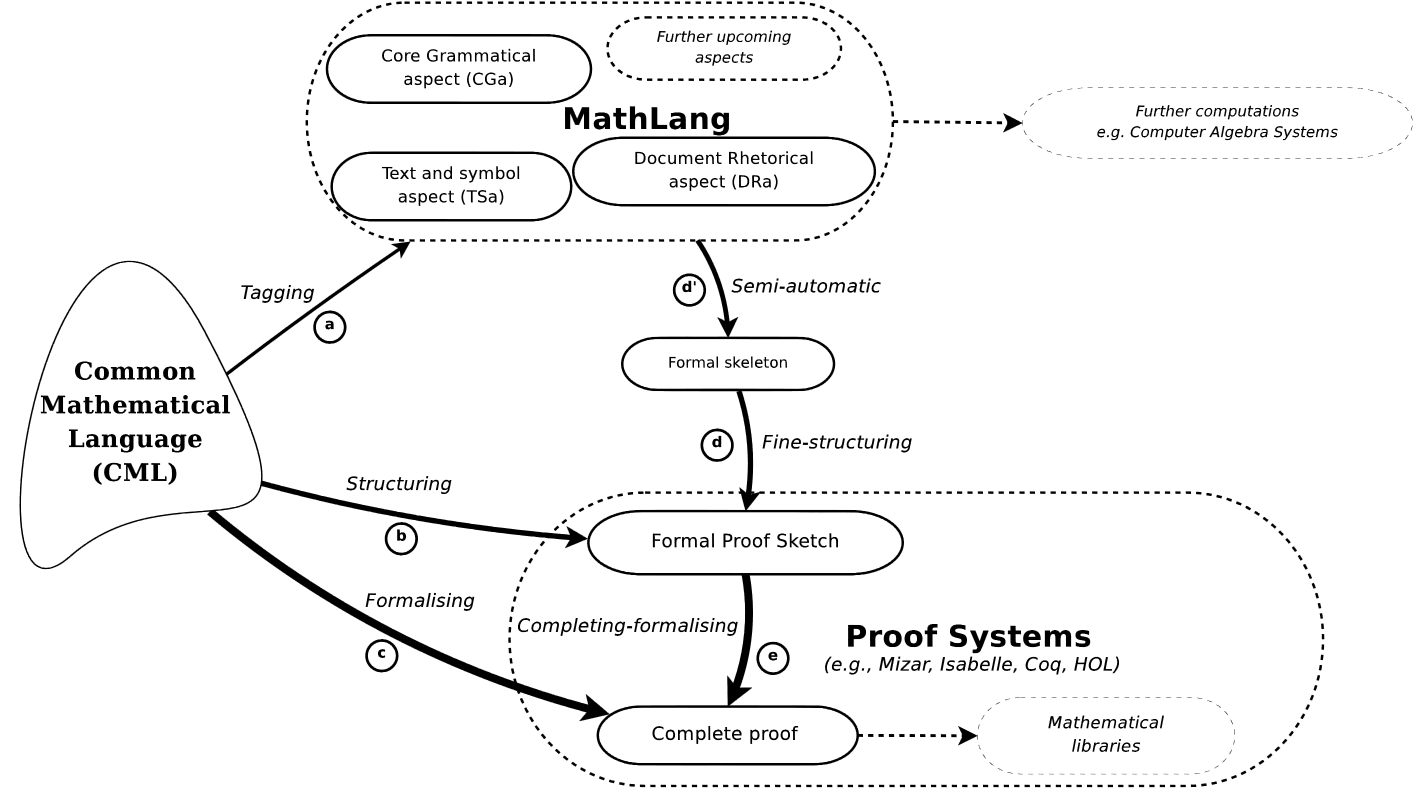
\includegraphics[scale=0.255]{Figures/Background/mathlang.png}
\end{center}
\caption{The MathLang approach to computerisation/formalisation \cite{mathintomizar}\label{fig:mathlang}}
\end{figure}

Figure \ref{fig:mathlang} shows the overall situation of work in the current MathLang Framework.
The labelled arrows show the computerisation paths from the common mathematical language to any proof system. The width of the arrow representing each path segment increases according to the expertise required to achieve the path segment. The level of expertise needed to computerise a CML text straight into a complete proof is very high, however the level of expertise is much smaller by using the MathLang framework to help form a formal skeleton and then into a complete proof. The dashed arrows illustrate further computerisation that one can envision.

\subsection{Core Grammatical aspect \label{subsec:cga}}
The current \gls{cga} in MathLang uses a finite set of grammatical \textit{categories} to identify the structure and common concepts used in mathematical texts. The aims of the \gls{cga} is to make explicit the grammatical role played by the elements of mathematical texts and to allow the validation of the grammatical and reasoning structure within the \gls{cga} encoding in a mathematical text. The \gls{cga} checks for grammatical correctness and finds errors like an identifier being used without and prior introduction or the wrong number of arguments being given to a function \cite{krzysztofphd}.

\subsection{Text and Symbol aspect \label{subsec:tsa}}
The \gls{tsa} builds the bridge between a mathematical text and its grammatical interpretation. The \gls{tsa} is a way of rewriting parts of the text so they have the same meaning. For example some mathematicians may prefer to write "a=b and b=c and c=d", others may prefer "a=b, b=c, c=d" and some others may prefer "a=b=c=d". As you can see all these methods of writing have the same meaning however some symbols are different. The \gls{tsa} annotates each expression in the text with a string of words or symbols which aim to act as the mathematical representation of which this expression is. This allows everything in the text to be uniform.

\subsection{Document Rhetorical aspect \label{subsec:dra}}

The Document Rhetorical aspects checks that the correctness of the reasoning in the mathematical document is correct and that there are no loops.The \gls{dra} mark-up system is simple and more concentrated on the narrative structure of the mathematical documents whereas other previous systems (such as DocBook \footnote{http://www.docbook.org}, Text Encoding Initiative \footnote{http://www.tei-c.org/index.xml}, OMDoc \footnote{http://www.omdoc.org}) were more concentrated on  the subtleties of the documents. It is used to describe and annotate chunks of texts according to their narrative role played within the document \cite{krzysztofphd}. Using the \gls{dra} annotation system we can capture the role that a chunk of text imposes on the rest of the document or on another chunk of text. This leads to generating dependency graphs which play an important role on mathematical knowledge representation. With these graphs, the reader can easily find their own way while reading the original text without the need to understand all of its subtleties. Processing \gls{dra} annotations can flag problems such as cicular reasoning and poorly-supported theorems.

\subsection{Full formalisation paths into Theorem Provers}

The MathLang project starts in 2000 when F.Kamareddine and J.B. Wells started the project within Heriot-Watt University as part of the ULTRA group \cite{researchprop}. It was an idea for a new mathematical language and framework to keep most of the advantages of Common Mathematical Language (CML) and avoid it's disadvantages. This framework would allow a gradual computerisation and formalisation of mathematical texts.

The framework was first set out in 2003 \cite{firstyear} and then saw an established path for conversion of a mathematical text written in CML into the isabelle proof assistant using rules and MathLang annotations \cite{secondyear}. A few short projects (by 4th year undergraduate dissertations or MSc students) have developed MathLang into the Framework it is today. A prototype of the Core Grammatical aspect and Text and Symbol aspect were defined in the PhD thesis of Manuel Maarek \cite{manuelphd} and then a gradual computerisation into the Mizar proof assistant using the three key aspects of MathLang were a great success and published \cite{mathintomizar}.

The design of the \gls{cga} is due to Kamareddine, Maarek and Wells \cite{oomathlang} and the implementation of the \gls{cga} is due to Maarek \cite{manuelphd}. The design of the \gls{tsa} is due to Kamareddine, Maarek, and Wells with contributions by Lamar to the souring rules \cite{restoringtsa}, \cite{manuelphd}, and \cite{lamarphd}. The implementation is primarily by Maarek \cite{manuelphd} with contributions from Lamar \cite{lamarphd}. The design and implementation of \gls{dra} were the subject of Retel's thesis \cite{krzysztofphd}. Further additions have since been carried out by Zengler \cite{cmtim}.

\subsection{Conclusion}
A lot of work has already been completed on the MathLang Framework. The three aspects, \gls{cga}, \gls{dra}, and \gls{tsa}, have been designed and redesigned so that a variety of mathematical texts and symbols could be used. Then the aspects have been implemented for ease of access. A translation from a mathematical text into the Mizar proof checker has been worked through and described in detail in a published paper \cite{mathintomizar} and a PhD thesis \cite{manuelphd}. A partial translation from a CML text into the Isabelle Syntax has also been carefully described in the 2009 paper \cite{mathintoisa} and also written in a PhD thesis \cite{lamarphd}. Some of the future work described was to allow MathLang to be used as a tool to computerise other pieces of information, such as another piece of academic text yet it does not need to be mathematical.

\section{Formal Methods in practice}
\label{sec:formnot}

Formal methods are mathematical approaches to software and system development which support the rigorous specification, design and verification of computer systems \cite{fmeurope}. Specifications are statements of how a proposed system should act and function. Formal methods use notations with defined mathematical meanings to describe specifications with prevision and no ambiguity. The properties of these specifications can then be works out with more confidence and can be described to the customers and other stakeholders. This then can uncover bugs in the stated requirements which they had not realised in a natural language specification. In this way a more complete requirements validation can take place earlier in the development life-cycle and thus save costs and time of the overall project. The rigor using formal methods eliminates design errors earlier and results in substantially redecued time \cite{benefitsofform}. 

Abrial presents two case studies in \cite{10.1145/1134285.1134406} describing the use of formal methods in industry. He concludes that one of the problems is that some managers are afraid that engineers will not be able to perform the interactive proofs. This thesis proposes to address this problem by inventing a method for a thereom proving novice to translate a formal specification into the theorem prover with little or no knowledge of the chosen theorem prover. The method proposed in this thesis provides an addition to testing and not a replacement. However the effort and costs should be reduced in the testing stages as the bugs would be found earlier in the specification and verification phase of the project. As well as giving the proposed system a highler level of rigor.

\subsection{The use of Formal Methods in Industry}

Despite these advantages some managers sometimes argue the cost of producing system using formal methods do not cover the costs. However the rigour using formal methods eliminates design errors earlier and results in substantially reduced time. Investing more effort in specifying, verifying and testing will benefit software projects by reducing maintenance costs, higher software reliability and more user-responsive software \cite{chantatub}.

Even in the 21st century we still experience a "software crisis" where software projects are being delivered far behind schedule, quality is poor and maintenance is expensive. Such software crisis allow for bad software to be released such as the computer system "Sabre" \cite{sabre}, which went off-line for almost a day leading to the cancellation of more then 700 flights.

Well engineered software is software which is suitable, efficient, reliable and maintainable with low costs and on schedule.

The cost of testing is around 50\% of the software cost. Maintenance cost is 2-4 times greater than pre-delivery cost. In large projects, failure to find and correct software errors can increase the cost of the software by 100 times, in small software projects it's usually about 2-4 times more.
More effort should be spent in requirements analysis and design to catch errors early in the project life-cycle \cite{andrewslides}. Computerising Z using the MathLang framework will do this as it is concentrating more on getting the requirement specifications correct and thus minimising errors later on in the project life cycle. For example, in the Sholis project \cite{sholis}, using a formal specification was most effective for fault finding, therefore if the specifications are correct, then the program implemented will in turn contain no grammatical errors if it follows the correct specification.

King, Hammond, Chapman and Pryor's paper \cite{sholis} was based on a project on the SHOLIS defence system. It highlighted the importance of having a Z specification on a system to check for errors. It was found that the Z proof was the most cost effective for fault finding. The Z specification found 75\% of the total faults for the system. Since Z specifications are important for finding faults in SIL4 systems (based on the sholis project), then checking the correctness of the Z specification is itself very important. Note that the specifications found 75\% of errors and not 100\%. As human error can still occur in formal specifications, using the ZMathLang approach may increase the percentage of errors found.

Hehner \cite{hehner99} also supports the use of specifications. He states it is the job of the specification to distinguish those things that are desirable in the program however when looking through a specification just with the human eye \cite{sholis} it is easy to make errors. Which is why checking the correctness of a specification through a theorem prover would help.

One reason industry is reluctant to use formal methods may be that they correctly perceive that the methods offered are too complicated for the benefits conferred. A way of simplifying the use of formal methods so that anyone in industry could understand would be a great benefit.

Hehner questions if all programs should have specifications. Which leads to the question of should simple programs also have specifications as well as high integrity systems. The benefits of planning and specifying a program far outweigh the time and cost of catching bugs and errors at a later stage \cite{planning} of complex programs. However it may be too time consuming for smaller program and it would be up to industry leaders themselves to decide.

Specifications, Programs, and Total Correctness \cite{hehner99} outlines that a programming language should not be the specification language. As not all industry experts are programming experts, the specification should be open for everyone in the team to understand the program not just the developers.

Hehner also states that total correctness is a mistake and partial correctness is enough. This may be because some software such as on aircraft's need to be running all the time when in the air and do not need to terminate. However with other programs it is important that they do terminate as a safety feature for example the Automatic track gauge changeover for trains \cite{automatictrain}. It is important that the program should terminate if anything should happen such as errors or a crash, therefore total correctness of only some programs is needed.

An Introduction to Proving the Correctness of Programs \cite{hantler} describes the specification of correct behaviour of a program by the use of input/output assertions. This would be very expensive in very large programs. So it may be good for smaller programs only. Assertion is a very basic approach.

However with this approach, checking for correctness can only be done by an expert in that particular programming language. They will have to understand where a procedure starts and where a procedure ends. By checking the correctness of specifications using the ZMathLang method it will allow for many program specifications to be checked by a wider audience and not just expert programmers.

The assumptions used in the example on page 336 \cite{hantler} resulted from an unresolved execution of the IF statement.

A paper reflecting on industry experience with proving properties in SPARK \ref{DBLP:conf/itp/ChapmanS14}, describes a programming language and verification system that will offer sound verification for programs. It states that SPARK and the use of proof tools remain a challange (published in 2014) as the `adoption hurdle' is percieved too high. Customers and regulators have taken a variety of stances on static analys and theorem provers. Where some places in industry have adopted the idea others remain sceptical. Hopefully this thesis will present an idea on how formal analysys could be simplified and broken up into smaller more understandable steps and thus would allow more users to take on the idea.

\section{Methods for checking for Software Correctness}

Traditionally, functional correctness has been obtained with pen and paper or an interactive proof assistant. Well-designed program verifiers are reducing the effort involved in doing full verifications.

Proof assistants soomestimes limit which program properties they reason about. By using the ZMathLang framework the specification would undergo different levels of rigor (and thus different types of checks) for example one might only want to check the grammatical correctness of the specification or one might want to fully formally prove the specification, different projects require different amounts of verification therefore the ZMathLang will allow this choice.

Dafny \cite{dafny} features modular verification, so that the separate verification of each part of the program implies the correctness of the whole program. This is similar to MathLang, Where Dafny checks different parts of the text and thus confirms correctness of the full text, \gls{math} checks the correctness of the text through different levels of rigor.

Dafny was able to do a proof for the code of Schorr-Waited Algorithm, however the writer states that the loop invariants are complicated because they are concrete. A refinement approach such as Jean-Raymond Abrials approach \cite{abrial} may be preferred. This thesis presents a way of creating proofs for the program specifications in the essence of Z \cite{essenceofz} using the MathLang steps.  

The Java modelling language in Dafny lacks an automatic verifier. An automatic verifier for modelling languages in this case would be beneficial as pen and paper verification could have a bugs dues to human error.

Another attempt at checking for correctness was written by Rex L.Page in Engineering Software Correctness \cite{engineeringsoftwarecorrectness}. A general theme within this paper, is that design and quality are important in engineering education. When teaching students how to create programs, it is not enough just to teach them how to develop software but to develop good quality software. This paper describes experiments with the use of ACL2 (a subset of lisp) with embedded on mechanical logic to focus on design and correctness. By using ACL2 it emphasises the importance of software design and correctness. 

ALC2 is coded therefore users must know how to code software to formulate proofs. The intention of ZMathLang is to allow many people in the development team to be able to formulate proofs such as project managers, designers, engineers etc. To do this, The MathLang steps (see section \ref{sec:mathlangbackground}) should be simple to do and simple to understand.

PVS (Prototype Verification System) \cite{pvs} is an environment for constructing specifications and developing proofs which have been mechanically verified. PVS has it's own specification language, which engineers would need to learn as well as using the environment for proofs. Type checking is undecidable for the PVS type system. The PVS also provides a language for defining high-level inference strategies.

Another tool which analysis the Z notation is Hol-Z \cite{hol-z}. It is a proof environment for Z. Hol-Z is embedded in Isabelle/HOL therefore it provides a type checking, documentation facilities and refinement proofs with a trusted theorem prover. Tools for formal specifications can be a implement a specification environment into a programming language and an embedded design which implements it into a theorem prover. The Z specification is implemented in \LaTeX{} then typed checked using an external plug in Zeta then transformed into sml files to be added into the Hol-Z theorem prover environment. The user will need to have some good expertise in the theorem prover Isabelle/Hol in order to fully prove the specification.

Fuzz \cite{spiveyfuzz} is a typechecker for the original Z language. It includes style files for \LaTeX{} and checks for the logical correctness of Z specification. This is different to the \gls{zcga} type checker as the weak types in \gls{zcga} check for the grammatical correctness and not the full logical correctness of Z. Therefore the grammatical correctness of partially formal specification can aslo be checked. The \gls{zmath} framework presented in this thesis uses the `zed' \LaTeX{} style package to typeset the Z specifications in the documents.


These tools are just some of the many Z tools available. There are many other tools for Z which can be found on the Z Notation Wikia page \cite{zwikia}. For this thesis we will concentrate on translating Z specifications into theorem prover Isabelle \cite{isabelle}. Isabelle is a generic proof assistant which allows mathematical formulas to be expressed in a formal language and includes numerous contributions worldwide. It contains a large mathematical toolkit (majority of Z can be represented in Isabelle) and has a lot of support in forms of documentation and online. It is distributed for free, easy to find, download and install and is regularly updated. The original \gls{math} has translated mathematical texts into Isabelle already (\cite{mathintoisa}) therefore we can use parts of that research to aid the research in this thesis.

\section{Proof carrying-code}

Proof carrying code is a framework for the mechanical verification of safety properties in machine language programs. The provider of the Proof Carrying Code (PCC) must provide both the executable code and a machine-checkable proof. This is to ensure the safety of the executable code so that it doesn't access any other data it is supposed to. However the machine-checkable proof is often very large and going through these errors in the machine checkable proof can be very labour intensive. Appel \cite{fpcc} attempts to make this an easier method by using foundational proof carrying code where he avoids any commitment to a particular type system or a verification checker. MathLang is similar to this method as the ultimate aim of ZMathLang is for the specification is to go through a correctness check step by step and only at the very end pick a verification checker to translate to. However all the steps until the final three (see figure \ref{fig:steps}) do not require the user to commit to a particular theorem prover.

PPC has several characteristics that allow it to execute foreign code safely. A critical components of any PCC implementation is the safety policy which is specified right at the start before any implementation takes place. This policy uses safety rules that the consumer of the machine code desires for any untrusted code. Proof carrying code is a two stage verification process \cite{suappc}. Using a "proof producer" and a "code consumer" to do the work. The proof producer must produce two kinds of work, one is the machine code and the other is the proof to verify that the machine code is safely executable. The ultimate aim of \gls{zmath} is to translate the specification of the system into a theorem prover for a proof of the specification. Proof carrying code is slightly different as the proof comes with the code. Since a large system may have lots of different components which join to make one large system. The proof carrying code would need to be implemented in all of the components (or the most safety-dependent) components. Formal specifications usually display the entire system and it's individual components. Therefore the entire system as a whole would be checked. However for a higher level of rigor one can use the ZMathLang framework to chec for the correctness as a whole system and then using proof carrying code to check the code itself for correctness.

Manish Mahajan \cite{pccman} explains that any implementation of proof carrying code must contain at least 4 elements: (1) a formal specification language used to express the safety policy, (2) a formal semantics of the language used by the untrusted code, (3) a language used to express the proofs and (4) an algorithm for validating proofs. MathLang's Document Rhetorical aspect and Core Grammatical aspect could partially formalise the formal specification needed to express the safety policy, (1), then the rest of the steps would be easier to follow as they will need to be less specific.

Using fast, effective proof checkers can increase the speed of execution of the binary when the consumer has the added overhead of verification of the proof. Mahajan writes that the size of binary will be increased due to inclusion of the safety proof which is a major area for research, this safety proof can be done during the formal specification, when designing the prototype of the system and thus minimizing the size of the safety proof needed for the PCC.

\section{Z Syntax and Semantics}

The Z notation is based upon set theory and mathematical logic. It is a particular formal method to which was originally developed to specify the new Customer Information Control System (CICS) functionality \cite{cics}. The set theory includes standard set operators, set comprehensions, cartesian products and power sets. Z also has other aspects such as schemas which are used to group mathematical objects and their properties. The schema language can be used to describe the state of a system and the ways in which that state may change \cite{Woodcock:1996:UZS:235337}.

In the Z notation there are two languages: the mathmatical language and the schema language. The mathematical language is used to describe various aspects of a design: object, and the relationships between them. The schema language is used to structure and compose descriptions: collecting pieces of information and naming them for re-use. A schema consists of two parts: a \emph{declaration part} and a \emph{predicate part}. Which consists of declared variables and their values respectively. We can write a schema either horizontally (figure \ref{fig:horizontalschema}) or vertically (figure \ref{fig:verticalschema}).

\begin{figure}[H]
\vspace{-0.2in}
\centering
\begin{minipage}{0.45\textwidth}
\begin{zed}
Schema\ Name \defs [declarations | predicates]
\end{zed}
\vspace{-0.18in}
\caption{An example of a schema written horizontally.\label{fig:horizontalschema}}
\vspace{-0.2in}
\end{minipage}\hfill
\begin{minipage}{0.45\textwidth}
\begin{schema}{Schema\ Name}
declarations
\where
predicates
\end{schema}
\vspace{-0.2in}
\caption{An example of a schema written vertically. \label{fig:verticalschema}}
\vspace{-0.2in}
\end{minipage}
\end{figure}

Therefore if we wanted a property of some system which consists of two variables $x$ and $y$ and state that $x$ must be smaller than $y$ then we can write:

\begin{schema}{xLessThany}
x: \nat \\
y: \nat
\where
x < y
\end{schema}

The full language of Z can be explored in \cite{spiveyreferencemanual}, \cite{essenceofz} and \cite{Woodcock:1996:UZS:235337}.

The semantics of Z specifications have already been studied. This has helped in the design of better specification languages by allowing critical comparison of specification techniques. As the basis semantics of Z have already been research, this gives us a head start in formulating the different aspects of \gls{math} for Z. The study in the semantics of Z provide a foundation for reasoning about specifications.

In \cite{formsem} it states that many of the proofs needed during the development process are `\textit{very shallow but contain a mass of detail}'. This detail would be difficult to understand by other stakeholders in the system being designed. This is where \gls{zmath} steps in, as it is a tool which produces documents in which anyone in the development team and clients should be able to understand.

The paper also states that \textit{consistency, completeness and refinement are essential to program development}. Therefore if the specification is consistent, complete and refined then the program will be as well (as long as the program sticks to the specification). Which makes it very important to have the specification checked as well as the program for errors. A formal semantics for the specification language is a necessary part of the specification of the software tools to support program development. Spivey also says that "theory  of signatures is decidable and therefore well suited to mechanical checking using a proof checker such as Mizar or Coq". However Mizar and Coq usually require a lot of expert level knowledge which leads to one of the aims of the thsis to break up the translation into smaller bitesize pieces to check for correctness of program specifications.

This thesis focuses on Ed Currie's, An Essence of Z \cite{essenceofz}. This would be a beneficial text to check for correctness as it only contains a subset of Z. Using the whole of Z may proof to be to difficult at the beginning as the syntax is very large and complicated, whilst starting with a small subset of Z and then expanding would be more efficient. The reason for this is because the framework developed in this thesis is for novices to get to grips with checking the correctness of Z and translating the specifications into a theorem prover. It does not promise to turn novices into theorem prover experts overnight but give them a guide with verifying the correctness of specifications. The research presented here is also not intended for theorem prover experts however users who are experts in theorem proving may also find some steps of the \gls{zmath} framework beneficial such as the \gls{zcga} or \gls{zdra}. The Essence of Z is also used as an academic text in undergraduate teaching and starts with very basics of logic to larger specifications which can be used a real software systems. It contains more then one specification and therefore gives a variety of syntax to use the MathLang framework on.

\section{Types and their desirable properties}

Type systems are good for many things \cite{pierce}, one of which includes that it allows early detection of some programming errors. Errors that are detected early can be fixed straight away rather then it lingering around to be discovered much later. Errors can often be pinpointed more accurately during type checking more often then in run-time, when their effects may not become visible until after some things go wrong, which in high integrity systems can have disastrous results. Type systems support the programming process by enforcing disciplined programming. Type system form the backbone of the module languages used to packaged and tie together all the different parts of large scale software systems. Types are also useful when reading programs. They form a useful documentation to the reader about the behaviour of the program, this form of documentation can not be outdated like comments since when the program specification changes so does the types involved.

Type-free lambda calculus \cite{bar93} allows for every expression to be applied to every other expression, eg I = $\lambda x.x$ may be applied to any argument $x$ to give the same result $x$. The expression may also be applied to itself. There are also typed versions of lambda calculus introduced by Curry \cite{cu34}. Types are usually objects of a syntactic nature and may be assigned to lambda terms. Using Types in this nature, this thesis describes a way in the \gls{zcga} (chapter \ref{ch:zcga}) assigns grammatical types to parts of a specification written in Z or partially written in Z. By doing so, the grammatical correctness of a system specification could be checked. The grammatical types are an adaptation from the grammatical categories taken from \cite{wtt}. One of the main benefits of the \gls{zcga} is it can check the grammatical correctness of partial formal specifications, that is specifications which are written in natural language and are on the way to becoming formal. Other Z type checkers such as Z/Eves \cite{Saaltink99thez/eves} and Fuzz \cite{spiveyfuzz} check the logical type correctness of a fully formalised Z specification.

\section{Generating properties to prove for Formal Specifications}

\begin{defin}
A logical formula associated to a correctness claim for a given verification property. The formula is valid if and only if the property holds. The correctness of the property under verification is “delegated” to proving the correctness of the new formula \cite{handbookofembed}.
\end{defin}

Therefore a proof obligation is a logical formular which the specifier must show to be a consequence of the specification so that a specification can be taken to be acceptable. In a more pragmatic sense proof obligations may be viewed as what the developer of a specification is obliged to prove in order to confirm that development is consistant.

Woodcock and Cavalcanti \cite{woodcock2004tutorial} use the alphabetised relational calculus to give denotational sematics to different constructs from programming patterns. This paper describes `\emph{healthiness conditions}' which identifies properties that characterise theries. Each one of these healthiness conditions represents a fact about the computational model for the programs being studied.

\begin{exam}
The variable `\emph{clock}' is an observation of the current time which is always moving onwards. The following predicate `B' specifies the clock variable:

\begin{zed}
B \defs clock \leq clock'
\end{zed}
\end{exam}

The healthiness condition described in this paper are specific proof obligations for the concept of \gls{utp}. The semantic model of \gls{utp} is presented a Z specification. Therefore the healthiness conditions for the specification would in one way be checking for the correctness of the \gls{utp} model. In a similar way, it is important to add healthiness conditions or as we call them in this thesis, `safety properties' in order to check each individual specification for various types of correctness.

Stepney describes two proof project written in Z in her paper a tale of two proofs \cite{stepney1998tale}. She explains how the proof process is deelply affected by \textbf{why} something is being proved, \textbf{what} is being proved and \textbf{how} the finished proof is to be presented. Stepney suggests that the proofs for specifications themselves do not have to be deep but the workings of what to proves can add to the labour. It is also important to keep in mind how deep the customer wants the proof and what level of assurance they need. She highlights 5 different points to prove:

\begin{figure}[H]
\begin{enumerate}
\item \textbf{Consistency checks}: Prove that your specification is cosistent and that it has a model.

\item \textbf{Sanity Checks}: In a `state and operations' style specification, prove that the state invariants are satisfied throughout and that the precondition of each operation is not \emph{false}.

\item \textbf{Emergent properties of a single specification}: Make explicit as a theorem some desired or suspected property of the specification, then prove it holds.

\item \textbf{Required properties of a single specification}: If some property is required to hold of the specification, and the specification has captured it implicitly, it needs to be made explicit and shown to hold.

\item \textbf{Properties across specifications}: Prove that a certain relationship holds between two specification such as the refinement relationship.
\end{enumerate}
\caption{Different points to prove in a specification \cite{stepney1998tale}. \label{fig:ptp}}
\end{figure}

Some of the points in figure \ref{fig:ptp} would be fairly easy to automate such as `consistancy checks' and `santity checks' however the other 3 points would be difficult to automate as they would all depend on the specification in question and would perhaps need some \emph{extra information} to decipher these properties. For example if one wish to automate proof obligations from point 5 the user would need to implement another specification (such as a refinement specification) and then prove the relationship between the original specification and the new one. In this thesis, we will concentrate on properties described in point 1 which have been automated. 

Stepney also explains that if the development process is incremental, it would be worthwhile getting a good structure for a proof up front which you can add more details in later. \gls{zmath}  can automatically generate this first structure which could be added to if needed. It can produce a specification in Isabelle syntax where other properties and details could be added to by the user at a later stage.

Most recently Mark Adams \cite{JFR4576} describes that even formalisation itself can be prone to error and therefore even if we do get a fully proven specification, the proof will also need to be checked. He outlines the flyspeck project which assists with the checking of formalised proofs. Adam calls this `\emph{proof auditing}', which adds another step of rigour to the theorem. \gls{zmath} assists with translating the specification into a theorem prover along with consistancy lemmas to prove. The user can then choose to prove these lemmas and the proof audit their thereom. However, even if proof auditting adds another level of rigour it is important to keep in mind who the user is doing the proofs for. As Stepney pointed out in \cite{stepney1998tale}, some clients wouldn't need that amount of rigor for their projects and only the proved safety properties may be enough.

Woodcock et al also describes that a specification can be developed in such a way that can lead to a suitable implementation called refinement \cite{Woodcock:1996:UZS:235337}. 

To refine a formal specification, more data must be added e.g. how certin calculations should be carried out. He states an abstract specification may leave design choices unresolved and its up to the refinement specificatino to resolve some of these choices. An example of this is shown in the following:

\begin{exam}

\begin{schema}{ResourceManager}
free: \mathbb{F} \nat
\end{schema}

 Any resource that is free can be allocated

\begin{schema}{Allocate}
\Delta ResourceManager \\
r!: \nat
\where
r! \in free \land free' = free \setminus \{r!\}
\end{schema}

\label{exam:allocate} 
\end{exam}

If there is more than one resource free in example \ref{exam:allocate} then this will class the specification as non deterministic.

Example \ref{exam:allocate} can be refined in that if there is more than one resource free, the resource with the lowest number should be allocated. This is shown in the following example:

\begin{exam}

\begin{schema}{Allocate}
\Delta ResourceManager \\
r!: \nat
\where
r! \in min~free \land free' = free \setminus \{r!\}
\end{schema}
\label{exam:allocaterefine} 
\end{exam}

Refining an abstract specification which is descibed in \cite{Woodcock:1996:UZS:235337} and in \cite{spiveyreferencemanual} is exactly what Stepney points out in point 5 from figure \ref{fig:ptp}. To show that this property holds the user would need to produce another specification which refines their original one and then include propertie of how they relate to eachoether. Since each individual specification is different then refinement specifications would be different to. Thus we wouldn't be able to automate this point. \gls{zmath} aims to assist the user in translating and proving their specification, the proof effort will be focused on properties which can be automated e.g. item 1 in figure \ref{fig:ptp}. Items 3, 4 and 5 would be to difficult to automate and therefore out of the scope of this thesis.

Fraser and banach describe .... in \cite{DBLP:conf/sefm/FraserB07} (Configurable Proof Obligations in the Frog Toolkit)

Then in \cite{DBLP:conf/icsea/WenMZ06} (Generating Proof Obligation to Verify Object-Z Specification),

\todo[inline]{Configurable Proof Obligations in the Frog Toolkit \cite{DBLP:conf/sefm/FraserB07},
Generating Proof Obligation to Verify Object-Z Specification \cite{DBLP:conf/icsea/WenMZ06}}

\section{Conclusion}
This chapter has described in depth the reasearch old and new which has relevence to this thesis. The MathLang framework which was designed and implemented for mathematics has been described and gives details of the method in which plain mathematical documents are formalised and translated into theorem provers. In this section we show a diagram which was proposed to identlify the steps in which a complete proof can be achieved from a mathematical text. 

The next section of this chapter highlights formal methods and formal languages used in practice. Formal methods which have been used in an industrial setting has been explained and analysed. We then outlined other methods for checking for software correctness which may or may not have been used in practice but also investigated in an academic setting.

Since this thesis concentrates on Z specifications we have outlined what are Z specifications and compared it with other formal languages. 

We also researched into types and their properties since the first aspect of \gls{zmath} is heavily based on a weak typing system.

This chapter concluded with different ways one can generate properties to prove their formal specifications.

\chapter{Overview of ZMathLang}
\label{ch:design}

Using the methodology of MathLang for mathematics (section \ref{sec:mathlangbackground}),
I have created and implemented a step by step way of translating Z
specifications into theorem provers with additional checks for correctness along
the way. This translation consists of one large framework (executed by a user
interface) with many smaller tools to assist the translation. Not only is the
translation useful for a novice to translate a formal specification into a
theorem prover but it also creates other diagrams and graphs to help with the
analysis of a formal system specification.

\begin{figure}[H]
 \begin{center}
 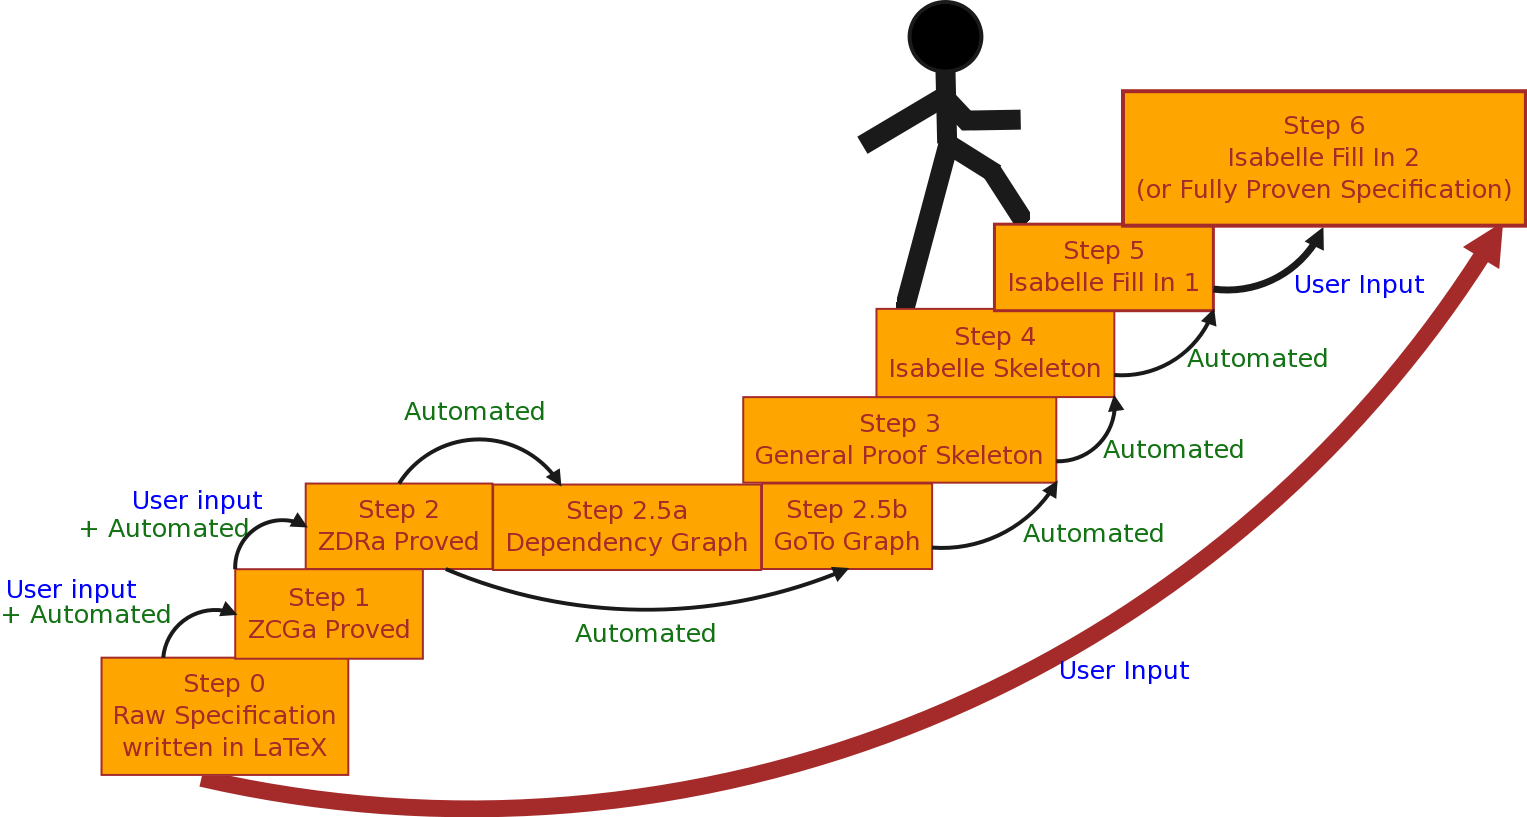
\includegraphics [width=12cm]{Figures/Design/mathlangsteps.png}
 \caption{The steps required to obtain a full proof from a raw specification.}
 \label{fig:steps}
\end{center}
\end{figure} 

The framework is targeted at beginners in theorem proving. The users should have
some idea of formal specifications but have no or little knowledge of the
targeted theorem prover. Figure \ref{fig:steps} shows the outline of the
framework. The higher the user goes up the steps the more rigorous the checks
for correctness. Step 1 and step 2 are interchangeable and can be done in any
order. However they both must be completed before moving up to step 3. Step 6 is
the highest level of rigour and checks for full correctness in a theorem prover.
For this thesis I have chose to translate Z specifications into Isabelle,
however this framework is an outline for any formal specification into any
theorem prover which could done in the future.

The user doesn't need to go all the way to the top to check for correctness, one
advantage of breaking up the translation is that the user gets some level of
rigour and can be satisfied with some level of correctness along the way.
However the main advantage of breaking up the translation is that the level of
expertise needed to check for the correctness of a system specification can be
done by someone who is not a theorem prover expert. This tool could also aid
users in learning theorem proving as it translates their specification and thus
they have examples of the syntax used in their theorem prover for their
specification. 

The arrows in figure \ref{fig:steps} represent the amount of expertise needed
for each step. In the last step, the arrow is slightly thicker as perhaps some
theorem prover knowledge would be needed to complete the proofs. However these
arrows are still small in comparison to the red thick arrow which represents
translating the specification all in one go.

The framework breaks the translation into 6 steps, most of which are partially
or fully automated. These are:

\begin{itemize}
\item Step 0: Raw LaTeX Z Specification. {\color{set}Start}
\item Step 1: Check for Core Grammatical correctness (ZCGa). {\color{set}User Input + Automated}
\item Step 2: Check for Document Rhetorical correctness (ZDRa). {\color{set}User Input + Automated}
\item Step 3: Generate a General Proof Skeleton (GPSa). {\color{set}Automated}
\item Step 4: Generate an Isabelle Skeleton. {\color{set}Automated}
\item Step 5: Fill in the Isabelle Skeleton. {\color{set}Automated}
\item Step 6: Prove existing lemmas and add more safety properties if needed. {\color{set}User Input}
\end{itemize}

\section{How far does the automation go?}

Figure \ref{fig:timeline} shows a diagram showing how far one can automate a
specification using automated \gls{zmath} and Isabelle tools. \Gls{zmath} is a
tool-set which assists the user in translating and proving a specification (going
from left to right). There are also other automating tools within Isabelle which
also assist the user with proving specifications (going from right to left) in
the diagram.

\begin{figure}[H]
 \begin{center}
 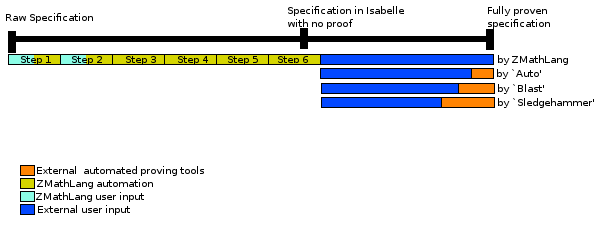
\includegraphics [scale=0.75]{Figures/Design/timeline.png}
 \caption{How far can one automate a specification proof.}
 \label{fig:timeline}
\end{center}
\end{figure} 

In figure \ref{fig:timeline} we show how far the user can get with automation
and how much work is still needed to get the full proof. \Gls{zmath} requires
user input for the first two steps (\gls{zcga} and \gls{zdra}) however the rest
up to step 6 is automated.

The black line shows the path going from a raw specification to a fully proven
specification with a milestone in the middle, which signifies when a
specification has been translated into Isabelle syntax but has no properties or
proof. \Gls{zmath} takes the user a little past this milestone as the tool-set
also generates properties to check the specification for consistency (see
section \ref{sec:proofobl}). These properties are added to the specification
during step 3 and continued throughout the translation. It is important to note
that the \gls{zmath} toolkit adds these properties to the translation but does
not prove them. That is why the rest of the \gls{zmath} path may require
external user input (dark blue) to complete the path. However, the \gls{zmath}
toolkit does assist the user in the translation past the halfway milestone on
the diagram.

We have created the \Gls{zmath} toolkit which assist the user from the
specification to full proof however there is also ongoing research on proving
properties from the theorem prover end. Figure \ref{fig:timeline} shows the
amount of proving techniques each automation holds. We have highlighted that
\gls{zmath} only gets the user so far in their proof however they are free to
use external automated theorem provers in completing their specification proof
if they so wish.

Even external automated theorem provers have their limitations. For example, the
user can use the Isabelle tool `\emph{sledgehammer}' to assist in solving
proofs, but not all can be solved by this technique. The sledgehammer
documentation advises to call `\emph{auto}' or `\emph{safe}' followed by
`\emph{simp\_all}' before invoking sledgehammer. Depending on the complexity of
ones proof, these sometimes may prove the users properties on their own, other
times it may not and the user will still need to invoke sledgehammer to reach
their goal. Sledgehammer itself is a tool that applies \gls{smt} solvers on the
current goal e.g. Vampire\cite{vampire}, SPASS \cite{fmintrol} and E \cite{e}. We
use sledghammer as a collective, to describe all the \gls{smt} solvers it covers
\cite{sledgehammer}.

Other automated methods include:

\begin{itemize}

\item \textbf{simp:} simplifies the current goal using term rewriting.

\item \textbf{arith:} automatically solves linear arithmetic problems.

\item \textbf{clarify:} like `\emph{auto}' but less aggressive.

\item \textbf{clarsimp:} a combination of `\emph{clarify}' and `\emph{simp}'.

\item \textbf{force:} like `\emph{auto}' but only applied to the first goal.

\item \textbf{auto:} applies automated tools to look for a solution.

\item \textbf{blast:} a powerful first-order prover. \cite{isacheat}
\end{itemize}

All these automated tools get increasingly more complex and cover more
properties, e.g \emph{clarsimp} covers more proving techniques then \emph{simp}
and \emph{blast} covers more proving techniques than \emph{auto} etc. With these
tools, one can prove certain properties about their theorem. However, there
still doesn't exist an automated proving tool which covers \textbf{all} proving
techniques. Therefore some user input will be required for more complex proofs.

\section{Overview of ZMathLang step by step}

This section gives an overview of each individual step in the \gls{zmath}
tool-set.

\subsection{Step 0- The raw LaTeX file}

The first step requires the user to write or have a formal specification they
wish to check for correctness. This specification can be fully written in Z or
partially written in Z (thus a specification written in English on it's way to
becoming formalised in Z). The specification should be written in \LaTeX{}
format and can be a mix of natural language and Z syntax. An example of a
specification written in the Z notation can be seen in figure
\ref{fig:zexample}.

\begin{figure}[H]
 \begin{center}
 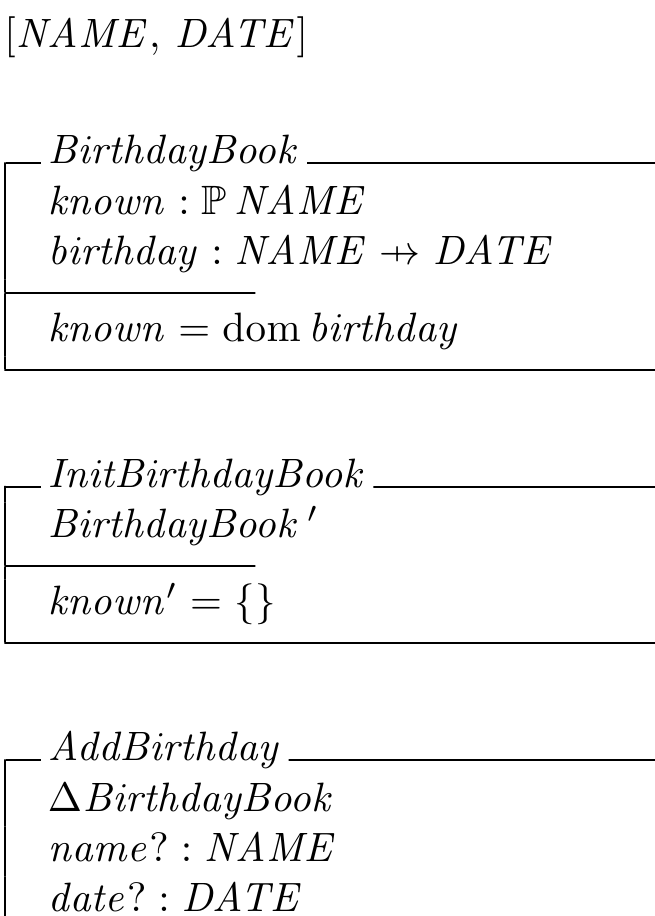
\includegraphics[scale=0.25]{Figures/Design/zspec.png}
 \caption{Example of a partial Z specification.}
 \label{fig:zexample}
\end{center}
\end{figure} 

\subsection{Step 1- The Core Grammatical aspect for Z}

The next step in figure \ref{fig:steps} shows that the specification should be
\gls{zcga} proved. Although this step is interchangeable with step 2 (\gls{zdra})
it is shown as step 2 on the diagram for convenience. In this step the user
annotates their document which they have obtained in step 0 with 7 grammatical
categories and then checks these for correctness. Figure \ref{fig:steps} shows
this step is achieved by user input and automation. The user input of this step
is the annotations and the automation is the \gls{zcga} checker. This
automatically produces a document labeled with the various categories in different
colours and can help identify grammar types to other members in the systems
project team. A \gls{zcga} annotated specification is shown in figure
\ref{fig:zcgaexample}. The \gls{zcga} is further explained in chapter
\ref{ch:zcga}.

\begin{figure}[H]
 \begin{center}
 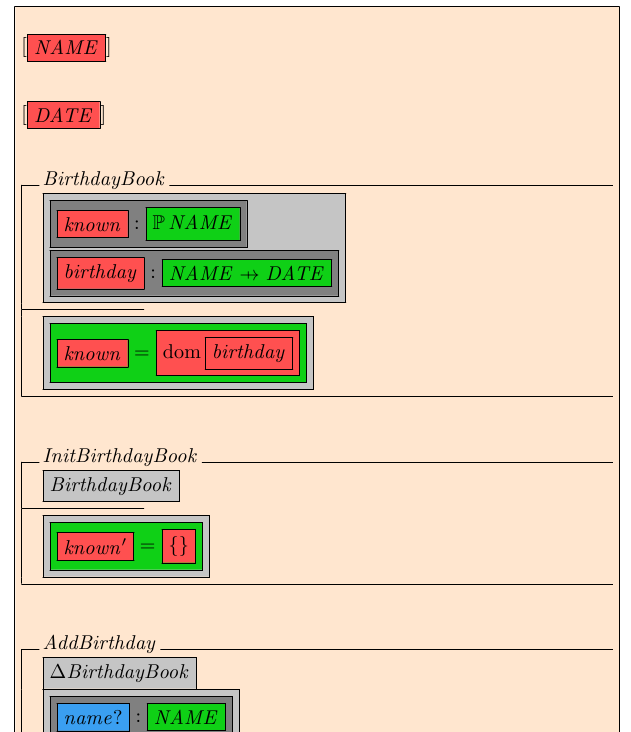
\includegraphics [scale=0.25]{Figures/Design/zcgaexample.png}
 \caption{Example of a ZCGa annotated specification.}
 \label{fig:zcgaexample}
\end{center}
\end{figure} 

\subsection{Step 2- The document Rhetorical aspect for Z}

The \gls{zdra} step, shown as step 2 in figure \ref{fig:steps}, comes before or
after the \gls{zcga} step. Similarly to the \gls{zcga} step, the user annotates
their document from step 0 or step 1 with \gls{zdra} instances and
relationships. This chunks parts of the specification together and allows the
user to describe the relationship between these chunks. The annotation is the
user input part of this step and the automation is the \gls{zdra} checker which
checks if there are any loops in the reasoning and gives warnings if the
specification still needs to be totalised. Once the user has annotated this
document and compiled it, the result shows the specification divided
into chunks and arrows showing the relations between the chunks. An example of a
Z specification annotated in \gls{zdra} is shown in figure
\ref{fig:zdraexample}. The \gls{zdra} is explained further in chapter
\ref{ch:zdra}.

\begin{figure}[H]
 \begin{center}
 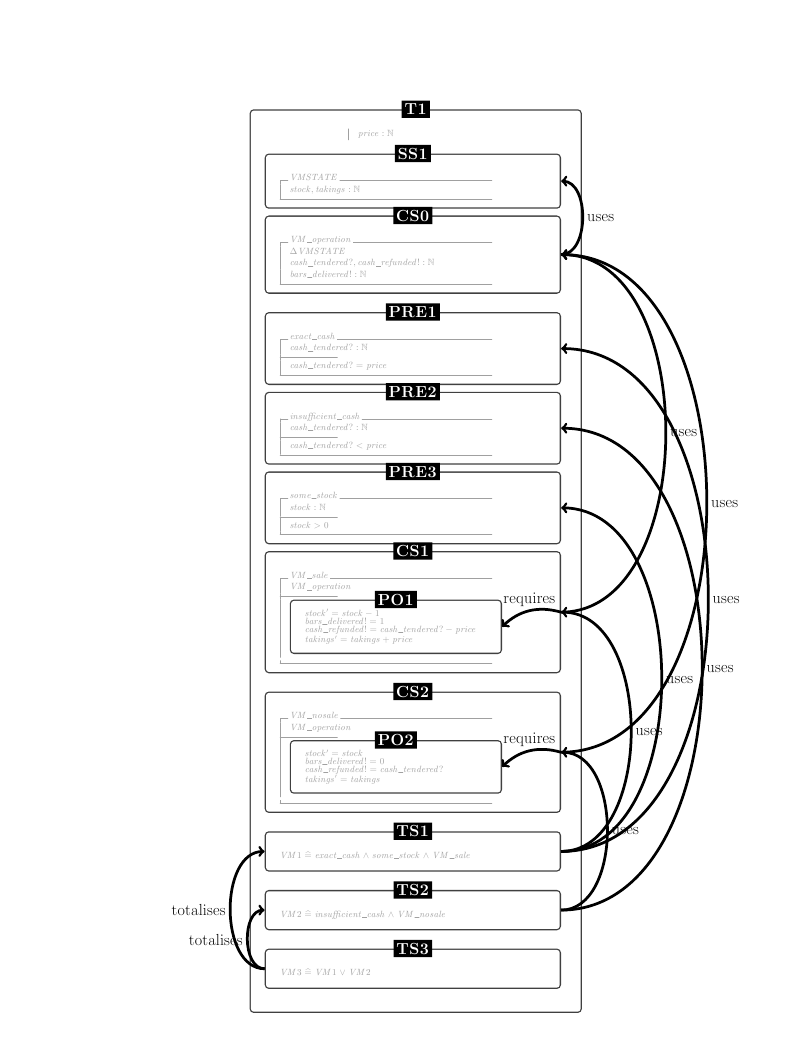
\includegraphics [scale=0.25]{Figures/Design/zdracomp.png}
 \caption{Example of a ZDRa annotated specification.}
 \label{fig:zdraexample}
\end{center}
\end{figure} 

The \gls{zdra} automatically produces a dependency and a goto graph (section
\ref{subsec:zdra_prodcuts}), these are shown as 2.5a and 2.5b respectively in
figure \ref{fig:steps}. The loops in reasoning are checked in both the dependency
graph and goto graph. An example of a goto graph is shown in figure
\ref{fig:gotoexamplee}.

\begin{figure}[H]
 \begin{center}
 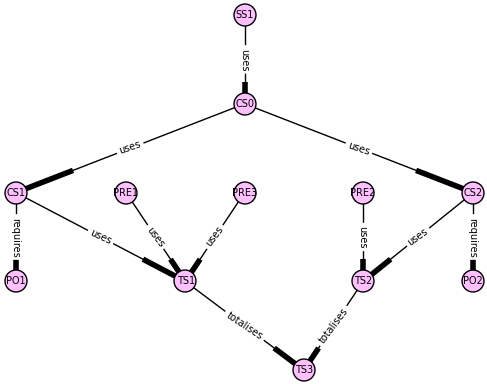
\includegraphics [scale=0.4]{Figures/Design/goto.png}
 \caption{Example of an automatically generated goto graph.}
 \label{fig:gotoexamplee}
\end{center}
\end{figure} 

\subsection{Step 3- The General Proof skeleton}

The following step is an automatically generated \gls{gps}. This document is
automated using the goto graph which is generated from the \gls{zdra} annotated
\LaTeX{} specification. It uses the goto graph to describe in which logical
order to input the specification into any theorem prover. At this stage it also
adds simple proof obligations to check for the consistency of the specification
i.e. the specification is consistent throughout. An example of a general proof
skeleton is shown in figure \ref{fig:proofskelexample}. The \gls{gps} is further
described in section \ref{sec:zdra2gen}.

\begin{figure}[H]
 \begin{center}
 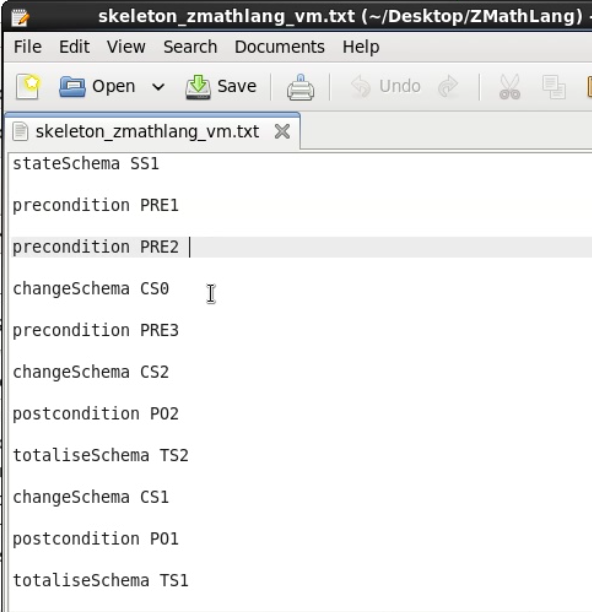
\includegraphics [scale=0.2]{Figures/Design/proofskel.png}
 \caption{Example of a general proof skeleton.}
 \label{fig:proofskelexample}
\end{center}
\end{figure} 

\subsection{Step 4- The Z specification written as an Isabelle Skeleton}

Using the \gls{gps} in step 3, the instances are then translated into an
Isabelle skeleton in step 4. That is, the instances of the specification are
translated into Isabelle syntax using definitions, lemma's, theory's etc to
produce a .thy file. This step is fully automated and thus a user with no
Isabelle experience can still get to this stage. An example of a Z specification
skeleton written in Isabelle is shown in figure \ref{fig:isaskelexample}.
Details of how this translation is conducted is described in chapter
\ref{chap:gpsa2isa} of this thesis.

\begin{figure}[H]
 \begin{center}
 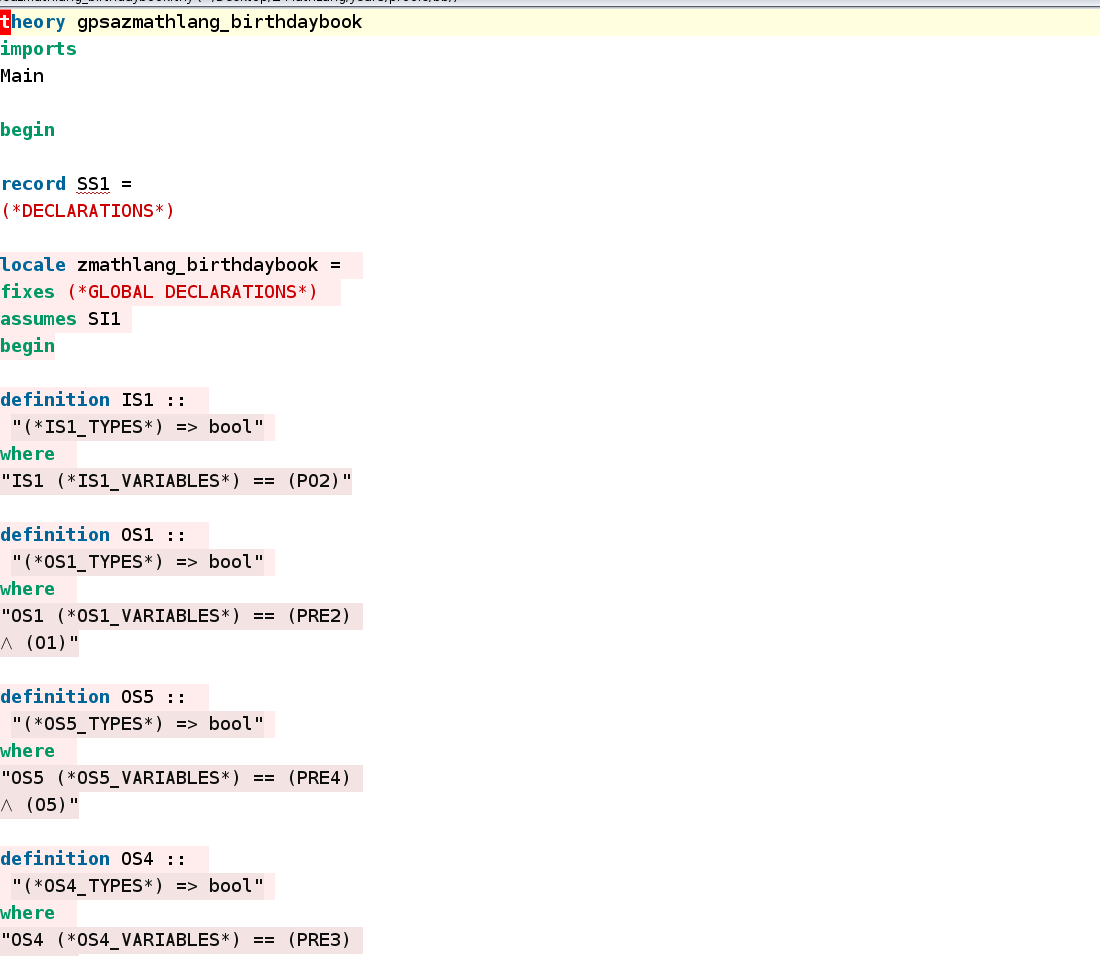
\includegraphics [scale=0.2]{Figures/Design/isaskeleton.png}
 \caption{Example of an Isabelle skeleton.}
 \label{fig:isaskelexample}
\end{center}
\end{figure} 

\subsection{Step 5- The Z specification written as in Isabelle Syntax}

Step 5 is also automated, using the \gls{zcga} annotated document produced in
step 1 and the Isabelle skeleton produced in step 4. This part of the framework
fills in the details from the specification using all the declarations,
expressions, definition etc in Isabelle syntax. Since the translation can also
be done on semi-formal specifications and incomplete formal specification there
may be some information missing in the \gls{zcga} such as an expression or a
definition. Note the lemmas from the proof obligations created in step 3 will
also be filled in, however the actual proofs for these will not and they will be
followed by the command `\texttt{sorry}' to artificially complete the proof. An
example of a filled in isabelle skeleton is shown in figure \ref{fig:fillin1}.

\begin{figure}[H]
 \begin{center}
 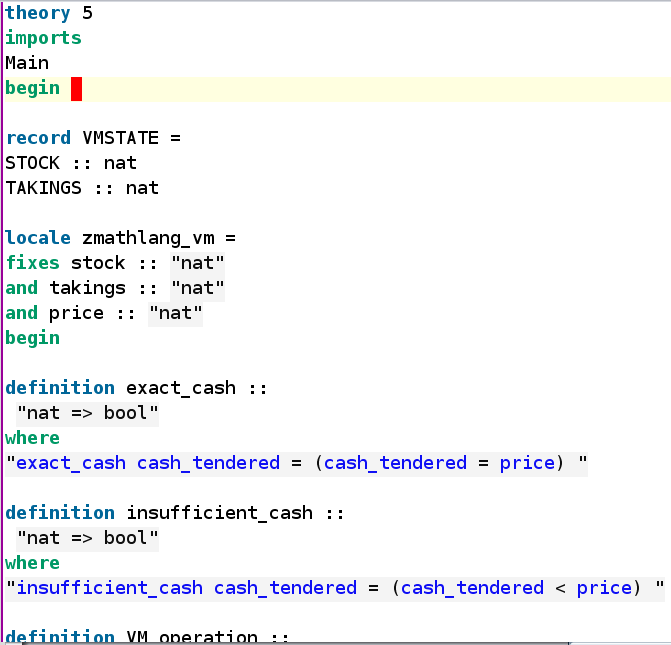
\includegraphics [scale=0.3]{Figures/Design/fillin1.png}
 \caption{Example of an Isabelle skeleton automatically filled in.}
 \label{fig:fillin1}
\end{center}
\end{figure} 

 If there is no \gls{zcga} information to fill in the Isabelle skeleton will not
 change. Further information on the translation is described in section
 \ref{sec:zcga2fillin} of this thesis.

\subsection{Step 6- A fully proven Z specification}

The final step in the \gls{zmath} framework (top of the stairs from figure
\ref{fig:steps}), is to fill in the Isabelle file from step 5. This final step
is represented by a slightly thicker arrow in figure \ref{fig:steps} compared
with the others as the user may need to have some little theorem prover
knowledge to prove properties. Also if there is some missing information such as
missing expressions and definitions the user must fill these out as well in
order to have a fully proven specification. However this may be slightly easier
then writing the specification from scratch as the user would already have
examples of other instances in their Isabelle syntax form. More details on this
last step is described in section \ref{sec:isa2ful} of this thesis.

\section{Procedures and products within ZMathLang}

\begin{figure}[H]
 \begin{center}
 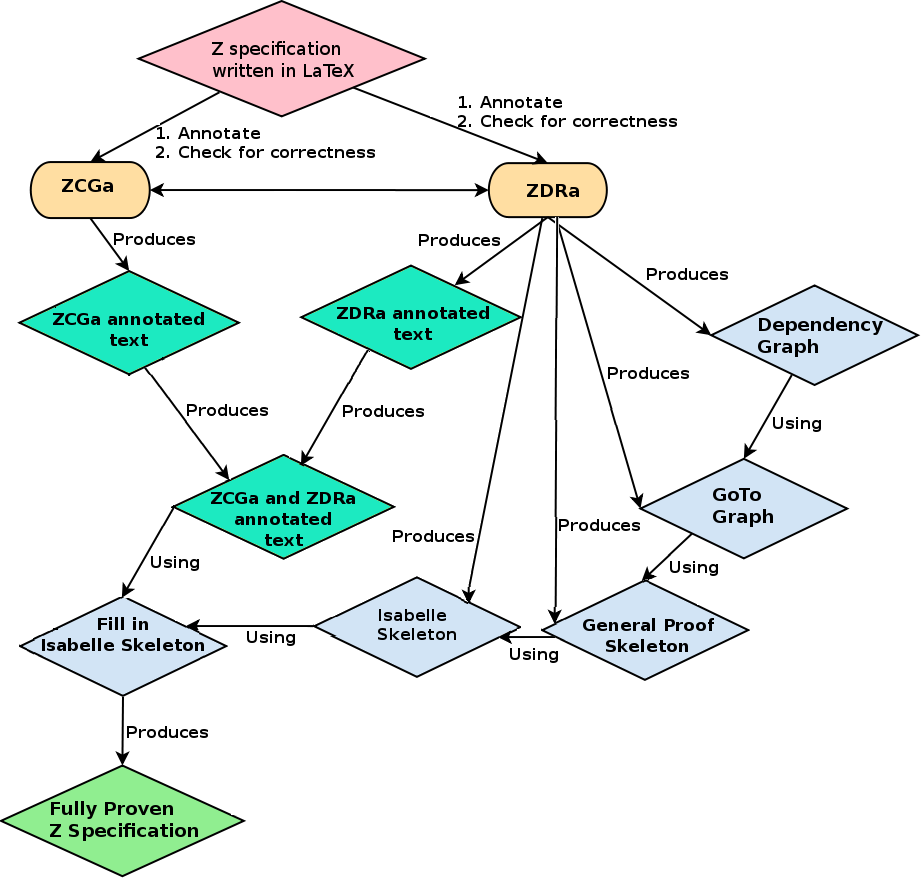
\includegraphics [scale=0.4]{Figures/Design/ZMathLangFlow.png}
 \caption{Flow chart of ZMathLang.}
 \label{fig:zmathflow}
\end{center}
\end{figure} 

Figure \ref{fig:zmathflow} shows a flow chart describing the documents produced
when using the framework and which documents are produced automatically,
semi-automatically and totally by the user. Products which are created by full
automation are diamonds in \colorbox{lightblue}{blue}. Diamonds in
\colorbox{lightgreen}{green} are produced by user input and products shown in
\colorbox{aqua}{aqua} diamonds are partial automated.

The \colorbox{lightpink}{pink} diamond is the starting point for all users. The
\colorbox{lightorange}{orange} ovals describe procedures of the ZCGa and ZDRa.
The ZCGa procedure requires user input and automation to produce a `ZCGa
annotated text'. The ZDRa procedure also requires user input and automation to
produce a `ZDRa annotated text'. Both the \gls{zcga} and \gls{zdra} procedures
done together produce a `\gls{zcga} and \gls{zdra} annotated text'. After
completing the \gls{zdra} procedure a 'dependency graph' is automatically
generated, which can then in turn generate a `GoTo graph' which in turn can
create a general proof skeleton. From the `general proof skeleton' we can then
create an `Isabelle skeleton'  which can be filled in using information from the
`\gls{zcga} and \gls{zdra} annotated text'. Using the `Filled in Isabelle
skeleton' the user needs to fill in the missing information and/or complete the
proofs in order to obtain a `fully proven Z specification'.

\section{The ZMathLang LaTeX Package}

The \gls{zmath} \LaTeX{} package (shown in appendix \ref{app:zmathlatex}) was
implemented to allow the user to label their Z specification document in
\gls{zcga} and \gls{zdra} annotations. Coloured boxes will then appear around
the grammatical categories when the new \gls{zcga} annotated document is
compiled with \texttt{pdflatex}. Instances and labelled arrows showing the
relations are also displayed when annotated with \gls{zdra} and compiled with
\texttt{pdflatex}. 

\subsection{Overview}

The \gls{zmath} style file invokes the following packages:

\begin{itemize}
\item tcolorbox - Used to draw colours around individual grammatical categories
with a black outline for the \gls{zcga}.
\item tikz - Used to identify the instances as nodes so the arrows can join from
one nodes to another.
\item varwidth - Used to chunk each instance as a single entity.
\item zed - Used to draw Z specification schemas, freetypes, axiomatic
definitions in the zed environment.
\item xcolor - Used to define specific colours and gives a wider range of
colours compared to the standard.
\end{itemize}

After invoking the packages we define the colours which are used in the
outputting pdf result. We use the same colours as the original \gls{math}
framework for the grammatical categories which are the same (sets, terms,
expressions, declarations, context and definitions) and choose a different
colour for the weak type `specification' as this hasn't been used in the
original \gls{math} framework.

\begin{figure}[H]

\includegraphics[scale=0.7]{Figures/Design/zmatha.png}
\caption{Part of the syntax to define the colours for \gls{zcga} in the \gls{zmath} \LaTeX{} file. \label{fig:definecolourlatex}}
\end{figure}

The command \verb|\definecolor{*NameOfZCGaType*}{HTML}{*ColourInHtml*}| is used
to define a colour for each grammatical category (shown in figure
\ref{fig:definecolourlatex}). Where \verb|*NameOfZCGaType*| is the name of the
category e.g. definition, term, set etc and \verb|*ColourInHtml*| is the HTML
number for the colour. For example the colour for term in the original
\gls{zmath} is \term{light blue} which in HTML format is \emph{3A9FF1}.
Therefore we define the colour for `\emph{term}' as \emph{3A9FF1}.

\subsection{\LaTeX{} commands to identify ZDRa Instances}

The \gls{zdra} section of the \LaTeX{} file provides three new commands:
\verb|\draschema|, \verb|\draline| and \verb|\dratheory|. The \verb|\dratheory|
annotation is for the entire specification which contains all the instances and
relations. The \verb|\draschema| command is to annotate the instances which are
entire zed schemas, this command should go before any \verb|\begin{schema}| or
\verb|\begin{zed}| command.

\begin{tabular}{|l | l|}
\hline
\verb|\draline{X}{\draschema{Y}{someContext}}| & {\color{set}Incorrect} \\
\hline
\verb|\draschema{Y}{\draline{X}{someContext}}| & {\color{set}Correct} \\
\hline
\end{tabular}

 The \verb|\draline| annotation is to annotate any instance that is a line of
 text which contains plain text or \gls{zcga} annotated text. But does not
 include any \gls{zdra} annotated text. For example in figure
 \ref{fig:zdraincorrectannotations} the \verb|\draline{PRE1}| annotation is
 embedded in the \verb|\draline{CS1}{| which will not compile. Therefore the
 correct way this schema is labelled is shown in figure
 \ref{fig:zdracorrectannotations} where the \verb|\draline{PRE1}| annotation is
 embedded in the \verb|\draschema{CS1}| annotation.

\begin{figure}[H]
\vspace{-0.2in}
\centering
\begin{minipage}{0.45\textwidth}
\centering
\begin{small}
\begin{BVerbatim}
\draline{CS1}{
\begin{schema}{B}
\Delta A
\where
\draline{PRE1}{a<b}
\end{schema}
}
\end{BVerbatim}
\end{small}
\vspace{-0.18in}
\caption{Incorrect annotating of \gls{zdra}.\label{fig:zdraincorrectannotations}}
\vspace{-0.2in}
\end{minipage}\hfill
\begin{minipage}{0.45\textwidth}
\centering
\begin{small}
\begin{BVerbatim}
\draschema{CS1}{
\begin{schema}{B}
\Delta A
\where
\draline{PRE1}{a<b}
\end{schema}
}
\end{BVerbatim}
\end{small}
\vspace{-0.2in}
\caption{Correct annotating of \gls{zdra}.\label{fig:zdracorrectannotations}}
\vspace{-0.2in}
\end{minipage}
\end{figure}

It is important to note this embedding order as by annotating a chunk of
specification using \verb|\draline| keeps everything inside as the \LaTeX{}
`\emph{math mode}'. Since the annotation \verb|\draschema| is outside the zed
commands (eg \verb|\begin{schema}|) it does not convert the content into
`\emph{math mode}' but the zed commands do.

\begin{figure}[H]
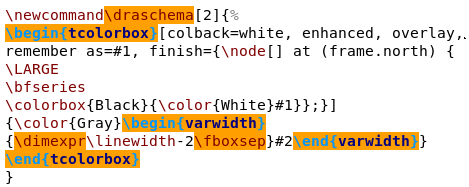
\includegraphics[scale=0.7]{Figures/Design/zmathb.png}
\caption{The syntax to define a \gls{zdra} schema instance in the \gls{zmath} \LaTeX{} file. \label{fig:latexzdraschema}}
\end{figure}

The new command we are defining for \verb|\draschema| is shown in figure
\ref{fig:latexzdraschema}. The commands for defining \verb|\dratheory| and
\verb|\draline| are similar as the \verb|draschema| definition. The command
takes two arguments, the first argument will be the name of the instance (e.g
SS1, IS4, CS2 etc) and the second argument is the instance itself. Any text
within the instance will then become grey so it looks faded as we are only
interested in the instance itself and not the context at this point. The
background of the box is white with a black outline. We then use the first
argument to name the instance and it becomes a node. The name of the instance is
also printed in black over the instance itself.

\subsection{\LaTeX{} commands to identify ZDRa Relations}

There are 5 new commands to define the relations for the \gls{zdra}, these are
\emph{initialOf}, \emph{uses}, \emph{totalises}, \emph{requires} and
\emph{requires}. Information on these relations are described in chapter
\ref{ch:zdra}, however this section of the thesis describes how the annotations
have been implemented in the \gls{zmath} \LaTeX{} package.

\begin{figure}[H]
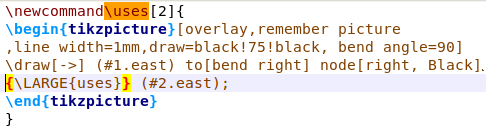
\includegraphics[scale=0.7]{Figures/Design/zmathd.png}
\caption{The syntax to define a \gls{zdra} schema relation in the \gls{zmath} \LaTeX{} file. \label{fig:latexzdrauses}}
\end{figure}

Figure \ref{fig:latexzdrauses} shows how the command \verb|uses| has been
implemented. The command takes 2 arguments (the should be 2 instances which have
been previously annotated) and draws an arrow going from the first instance to
the second one. The arrow bend angle is at 90, the arrow width is at 1mm and the
arrow goes from the east part of the first instance to the east part of the
second instance. The word \textbf{uses} is written next to the arrow. All the
other relation commands are written in a similar way however the direction of
the arrows differ and some arrows bend to the left whilst others bend to the
right. The bending of the arrows has been implemented at random so that the
compiled document has arrows showing on both sides of the theory and are not
overlapping too much.

\subsection{\LaTeX{} commands to identify ZCGa grammatical types}

The \gls{zcga} part of the \LaTeX{} file package uses the colours previously
defined in the style file. To define each of the grammatical types we use the
\texttt{fcolorbox} command. This creates a black outline and a coloured
background for each of the grammatical categories.

\begin{figure}[H]
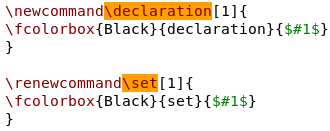
\includegraphics[scale=0.7]{Figures/Design/zmathe.png}
\caption{The syntax to define a \gls{zcga} grammatical categories. \label{fig:latexzcga}}
\end{figure}

Figure \ref{fig:latexzcga} shows the commands to define the coloured boxes for
\emph{declaration} and \emph{set}. As set is already defined in the mathematical
\LaTeX{} library, we renew the command. The command takes one argument (the text
the user which to annotate), changes it to mathmode and draws the box around it.
All the grammatical categories are defined in the same way, each with their own
background colour. The only exception is the grammatical category of
\emph{specification} as this command does not convert the specification into
mathmode.

\section{Conclusion}

In total there are 6 steps in order to translate a Z specification into the
theorem prover Isabelle. These steps have been designed so that the system
engineer/system designer of the project could use them.  Each of these steps
assist the user in understanding the specification, and some steps even produce
documents, graphs and charts in order to analyse the specification. These
products also allow others in the development team to understand the system
better such as clients, stakeholders, developers etc. The majority of the steps
are fully automated whilst some a little user input. Each step checks for some
form of correctness and becomes more and more rigorous each step the user takes
towards step 6. The next chapter begins to describe step 1 (\gls{zcga}) in more
detail.
%\chapter{Z Core Grammatical aspect}
\label{ch:zcga}

The \gls{zcga} is a weak type checker, which checks for grammatical correctness
in formal Z specifications and partially formalised Z specifications. It is not
the same as pure Z type checkers as it only checks the grammar on a sentence
level and not the logical correctness. The \gls{zcga} has it's roots in weak
type theory for mathematics \cite{wtt}. Core grammatical correctness for Z has
also adapted the rules from the \gls{cga} for mathematics (see section
\ref{sec:mathlangbackground} in chapter \ref{ch:background}).

This chapter focuses on the first step of the \gls{zmath} tool-set. The user can
check for grammatical correctness with the aim to translate the specification
fully into a theorem prover or they can use this step on it's own to check their
specification for some level of rigor.

The first part of this chapter explains the design of the \gls{zcga} and how the
rules and categories have been adapted from \cite{wtt}. It gives some examples
of each of the categories and how they are used in Z. We then explain the rules
in which the categories must follow in order to be \gls{zcga} correct. The next
section highlights some properties we can show about the \gls{zcga}. Then we
explain how the categories of the \gls{zcga} syntax are converted into weak
types and check Z specifications for grammatical correctness.

The final section demonstrates the implementation of the \gls{zcga} and gives
examples of certain errors one can get when checking a specification for
grammatical correctness.

\section{Weak Types}

Since formal notation is a subset of mathematics we are able to adapt the
\gls{cga} for mathematics to work for formal specification and thus the Z
notation.

In order to check for grammatical correctness we introduce a weak type system
for Z specifications illustrated in figures \ref{tab:zcga1}.
 
The ZCGa starts from it's lowest level, the \emph{atomic level}, which
underlines the elementary characters from which the syntax is made. It then
builds itself up to the highest level, \emph{discourse level} where the largest
elements can be found. Everything in the \emph{discourse} can be made from
elements in the smaller levels. Everything in the \emph{sentence level} can be
made from the levels before and so on. Types in Z are not the same as weak
types. Therefore we shall name each of the weak types, categories to eliminate
confusion.

\begin{table}[H]
\begin{tabular}{|l || l | l | c|}
\hline
level & Main category & syntax & Meta-symbol\\
\hline
& \textit{variables} & $V = V ^ {\mathcal{T}} \vert V ^ {\mathbb{S}}$ & x  \\
atomic & \textit{constants} & $C = C ^ {\mathcal{T}} \vert C ^ {\mathbb{S}}
\vert C ^ \mathcal{E}$ & c  \\
& \textit{binders} & $B = B ^ {\mathbb{S}} \vert B ^ \mathcal{E}$ & b \\
\hline
phrase & \textit{terms} & $\mathcal{T}$ =
$C^{\mathcal{T}}(\overrightarrow{\mathcal{P}})$  $\vert V ^ {\mathcal{T}}$ & t
\\
 & \textit{sets} & $\mathbb{S}$ =
 C$^{\mathbb{S}}(\overrightarrow{\mathcal{P}}$)$\vert
 B^{\mathbb{S}}_{\mathcal{Z}}(\mathcal{E}) \vert V^\mathbb{S}$ & s \\
\hline
sentence & \textit{expressions} & $\mathcal{E}$ =
$C^{\mathcal{E}}(\overrightarrow{\mathcal{P}}) \vert
B^{\mathcal{E}}_{\mathcal{Z}}(\mathcal{E})$ & E  \\
& \textit{definitions} & $\mathcal{D} = C^{\mathbb{S}}(\overrightarrow{V}):=
\mathbb{S}$ & D \\
\hline
discourse & \textit{schematext} & $\mathbf{\Gamma}$ = $\emptyset \vert
\mathbf{\Gamma}, \mathcal{Z} \vert \mathbf{\Gamma}, \mathcal{E}$ & $\Gamma$\\
& \textit{paragraphs} & $\Theta$ = $\mathbf{\Gamma} \triangleright \mathcal{E}
\vert \mathbf{\Gamma} \triangleright \mathcal{D}$ & $\theta$\\
& \textit{specifications} & \textbf{Spec} = $\emptyset \vert \mathbf{Spec},
\Theta$  & spec \\
\hline
\end{tabular}

\begin{tabular}{|l|l|c|}
\hline
Other Category & abstract syntax & Meta-symbol\\
\hline
\textit{parameters} & $\mathcal{P} = \mathcal{T} \vert \mathbb{S} \vert
\mathcal{E}$ & P\\
\textit{declarations} & $\mathcal{Z}$ = V$^{\mathbb{S}}$:SET $\vert$
V$^{\mathcal{T}}$:$\mathbb{S}$ & Z\\
\hline
\end{tabular}

Note: $\overrightarrow{\mathcal{P}}$ is a list of 0 or more $\mathcal{P}$'s,
$\overrightarrow{\mathbb{S}}$ is a list of 0 or more $\mathbb{S}'s$,\\
$\overrightarrow{\mathcal{E}}$ is a list of 1 or more $\mathcal{E}'s$,
$\overrightarrow{V}$ is a list of 0 or more $V's$.
\caption{Categories of ZCGa syntax.} \label{tab:zcga1}
\end{table}

We use some of the weak types in \cite{wtt} in our weak types for Z. In
particular \emph{book} becomes \emph{specification}, \emph{lines} become
\emph{paragraphs}, \emph{context} becomes \emph{schematext} and
\emph{statements} become \emph{expressions}. We eliminate \emph{nouns},
\emph{adjectives} and only have one syntax for \emph{definition}.

\subsection{Examples of specifications and weak types}
Everything within a Z specification can be labelled using the categories found
in table \ref{tab:zcga1}.

\begin{figure}[H]
\centering
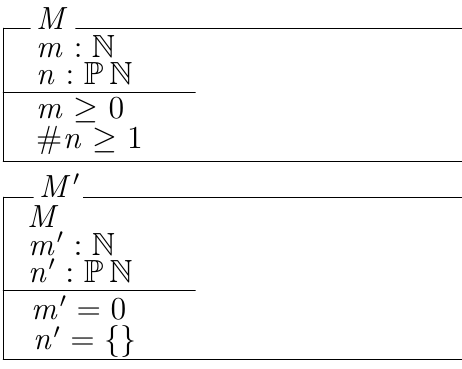
\includegraphics[scale=0.4]{Figures/zcga/toy.png}
\caption{Basic example of a specification \label{fig:toy}}
\end{figure}

Using figure \ref{fig:toy} we will give examples of individual weak type
categories.

\paragraph{variables}
\label{subsubsec:variables}

The set of variables $V$ is divided into two subsets $V^{\mathcal{T}}\text{ and
} V^{\mathbb{S}}$ which correspond to variables giving terms and variables
giving sets respectively.

\begin{itemize}
\item $V^{\mathcal{T}}$. An example of a variable giving a term would be `$m$'
in figure \ref{fig:toy}.

\item $V^{\mathbb{S}}$. An example of a variable giving a set would be `$n$' in
figure \ref{fig:toy}.
\end{itemize}

\paragraph{constants}
\label{subsubsec:costants}

The set of constants range over constants giving terms $C^{\mathcal{T}}$,
constants giving sets $C^{\mathbb{S}}$ and constants giving expressions
$C^{\mathcal{E}}$.

\begin{itemize} 
\item $C^{\mathcal{T}}$. An example of a constant giving a term would be `$0$'
in figure \ref{fig:toy}.

\item $C^{\mathbb{S}}$. An example of a constant giving a set would be `$\{\}$'
in figure \ref{fig:toy}.

\item $C^{\mathcal{E}}$. An example of a constant giving an expression would be
`$m' = 0$' where the constants is `$=$' from figure \ref{fig:toy}.
\end{itemize}

\paragraph{binders}
\label{subsubsec:binders}

There are two subsets of binders in the categories for Z specifications. Binders
giving sets $B^{\mathbb{S}}$, and binders giving expressions $B^{\mathcal{E}}$.

\begin{itemize}
\item $B^{\mathbb{S}}$. An example of a binder giving an expression is 
\newline
\noindent `$\exists schedule:TIMESLOT \leftrightarrow ROOM \bullet (allPairs
moduleTT \cap schedule = \emptyset \land moduleTT = moduleTT \oplus {m? \mapsto
schedule})$'
\newline
\noindent taken from Timetable specification in \cite{mathlangexamples}.

\item $B^{\mathcal{E}}$. An example of a binder giving a set is
\newline
\noindent `$\bigcup \{s:\dom studentTT \bullet \{s \mapsto (studentTT~s
\setminus moduleTT~m?)\}$' \newline
\noindent taken from Timetable specification in \cite{mathlangexamples}.
\end{itemize}

\paragraph{terms}
\label{subsubsec:terms}

Terms can range over constants giving terms with optional parameters
$C^{\mathcal{T}}(\overrightarrow{\mathcal{P}})$, and variables giving terms
$V^{\mathcal{T}}$.

\begin{itemize}
\item $C^{\mathcal{T}}(\overrightarrow{\mathcal{P}})$. An example of a constant
giving a term is `$\# n$' (taken from figure \ref{fig:toy}) the constant being
$\#$ which would be in the preface of constants with the weak typing as
$\mathbb{S} \rightarrow \mathcal{T}$ and the parameter of this constant giving a
term would be `$n$' which is set.

\item $V^{\mathcal{T}}$. See section \ref{subsubsec:variables} on variables
giving terms.
\end{itemize}

\paragraph{sets}
\label{subsubsec:sets}

The category of \emph{set} has three sub categories, constants giving sets with
optional parameters $C^{\mathbb{S}}(\overrightarrow{\mathcal{P}})$, binders
giving sets with expression as its parameter
$B^{\mathbb{S}}_{\mathcal{Z}}(\mathcal{E})$ and variables giving sets
$V^{\mathbb{S}}$.

\begin{itemize}
\item $C^{\mathbb{S}}(\overrightarrow{\mathcal{P}})$. An example of a constant
giving a set with parameters is
\newline
`$studentTT = studentTT \union {s? \mapsto \emptyset}$'
\newline
taken from Timetable specification in \cite{essenceofz}. Where the
constant giving a set is `$\union$' and the parameters it takes is `$studentTT$'
and `${s? \mapsto \emptyset}$'.

\item $B^{\mathbb{S}}_{\mathcal{Z}}(\mathcal{E})$. An example of a binder giving
a set with an expression and declaration as parameters is
\newline

`$\bigcup \{s:\dom studentTT \bullet \{s \mapsto (studentTT~s \setminus
moduleTT~m?)\}\}$' \newline
taken from Timetable specification in \cite{essenceofz}. Where the
constant is `$\bigcup$', the declaration parameter is `$s:\dom studentTT $' and
the expression parameter is `$  \{s \mapsto (studentTT~s \setminus
moduleTT~m?)\}$'.

\item $V^{\mathbb{S}}$. See section \ref{subsubsec:variables} on variables
giving sets.
\end{itemize}

\paragraph{expressions}
\label{subsubsec:expressions}

The category of expressions ranges over two subsets, constants giving
expressions with optional parameters
$C^{\mathcal{E}}(\overrightarrow{\mathcal{P}})$, and binders giving expressions
with a declarations and expression $B^{\mathcal{E}}_{\mathcal{Z}}(\mathcal{E})$.

\begin{itemize}
\item $C^{\mathcal{E}}(\overrightarrow{\mathcal{P}})$. A constant giving an
expression can be seen in figure \ref{fig:toy} as `$m \geq 0$' where `$\geq$' is
the constant giving an expression and the parameters are two terms: `$m$' and
`$0$'.

\item $B^{\mathcal{E}}_{\mathcal{Z}}(\mathcal{E})$. A binder giving an
expression could be a `$\forall$' or `$\exists$' binder. An example of this is
shown in the Timetable specification in \cite{essenceofz} as
\newline
`$\exists schedule : TIMESLOT \leftrightarrow ROOM \bullet(allPairs moduleTT
\cap schedule = \emptyset \land moduleTT = moduleTT \oplus \{m? \mapsto
schedule\})$'
\newline
where the binder giving an expression is `$\exists$', the declaration parameter
is `$TIMESLOT \leftrightarrow ROOM$' and the binding expression is `$(allPairs
moduleTT \cap schedule = \emptyset \land moduleTT = moduleTT \oplus \{m? \mapsto
schedule\})$'.
\end{itemize}

\paragraph{definitions}
\label{subsubsec:definitions}

Theres is only one kind of definition in the weak type theory syntax for Z. A
local definition in Z is a constant giving a definitions taking variables as
parameters giving a set, $C^{\mathbb{S}}(\overrightarrow{V}):= \mathbb{S}$. An
example of this is shown the GenDB specification in \cite{essenceofz}.
The definition is
\newline
 `$\mathbf{let}\
 cosrel==(parent^{nth?+1}\comp(parent^{-1})^{nth?+1+rem?})\setminus (parent
 \comp parent^{-1}) \bullet$\newline
\indent $cousins! = cosrel \limg \{p?\}\rimg \union cosrel^{-1} \limg \{p?\}
\rimg$'
\newline
where the defined constant is $cosrel$.

\paragraph{schematext}
\label{subsubsec:schematext}

The schematext within a Z specification reigns over three sub categories,
either the schema text can be empty $\emptyset$, or it can be schematext with a
declaration $\mathbf{\Gamma}, \mathcal{Z}$ or it can be schematext with an
expression $\mathbf{\Gamma}, \mathcal{E}$.

\begin{itemize}
\item $\emptyset$. The empty schema text is the beginning of a specification
where we start with nothing.

\item $\mathbf{\Gamma}, \mathcal{Z}$. The first declaration in a specification
would be the empty $\Gamma$ plus the declaration. For example in figure
\ref{fig:toy} the first example of this would be `$m:\nat$', which is the empty
schematext $\emptyset$ along with the first declaration of the specification.
The second declaration add to the schema text would be $n:\power \nat$ and so
on.

\item $\mathbf{\Gamma}, \mathcal{E}$. This set represents all the expressions
which are added to the schema text. In the example in figure \ref{fig:toy} we
would already have two declarations in the schematext $m:\nat$ and $n:\power
\nat$ in the schema text before the first expression is added $m \geq 0$. The
second expression added to the schematext in the same example would be $\# n
\geq 1$. 

\end{itemize}

\paragraph{paragraphs}
\label{subsubsec:paragraphs}

A paragraph $\Theta$ contains either an expression $\mathbf{\Gamma}
\triangleright \mathcal{E}$ or a definition $\mathbf{\Gamma} \triangleright
\mathcal{D}$, relative to a schematext.

The symbol $\triangleright$ is a separation marker between the schematext and
expression or definition

\begin{itemize}
\item $\mathbf{\Gamma} \triangleright \mathcal{E}$. Examples of expressions in a
paragraph see section \ref{subsubsec:expressions}.

\item $\mathbf{\Gamma} \triangleright \mathcal{D}$. Example of definitions in a
paragraph see section \ref{subsubsec:definitions}.
\end{itemize}

\paragraph{specifications}
A specification $spec$ is a list of paragraphs: $spec= \emptyset \vert
\mathbf{Spec}, \Theta$.

A simple example of a specification is the entire of figure \ref{fig:toy}.

\paragraph{other categories}

Here we describe the other categories which are needed in the \gls{zcga}
abstract syntax.

\paragraph{Declarations.} A declaration ina schematext represents the
\emph{introduction of a variable} of a known type. In the categories of ZCGa
syntax we can have two different kinds of declarations. This can be:
\texttt{SET} (the type of all sets) or a set. Both of these declarations relates
a \emph{subject} (the left hand side of the declaration) with its
\emph{type/predicate} (right hand side of the declarations). The abstract syntax
for the two categories of declarations are $V^{\mathbb{S}}$ is a set
$V^{\mathbb{S}}:SET$, or term $V^{\mathcal{T}}$ is in the set $\mathbb{S}$,
$V^{\mathcal{T}:\mathbb{S}}$.

\begin{itemize}
\item$V^{\mathbb{S}}:SET$. An example of this kind of declaration is `$n':\power
\nat$' taken from figure \ref{fig:toy}.

\item $V^{\mathcal{T}:\mathbb{S}}$. An example of this kind of declaration is
`$m:\nat$' taken from figure \ref{fig:toy}.
\end{itemize}

\paragraph{Parameters.} The list of parameters represent the categories in which
constants may depend. The parameters available in the \gls{zcga} abstract syntax
are terms $\mathcal{T}$, sets $\mathbb{S}$ or expressions $\mathcal{E}$. For
details on how each of these parameters are formed see the relevant sections
(\ref{subsubsec:terms}, \ref{subsubsec:sets} and \ref{subsubsec:expressions}
respectively).

\subsection{Weak Typing Rules}

The ZCGa uses the weak types found in table \ref{tab:zcga1} and checks the
specification is correct according to the rules found in \ref{tab:wttrules}. To
write the rules for the \gls{zcga} we must first establish some definitions. The
following definitions have been adapted from \cite{wtt} to accommodate Z
specifications.

\begin{defin}
We abbreviate $\vdash$ spec $\mathbf{::Spec}$, spec $\vdash \Gamma
\mathbf{::\Gamma}$ as OK(spec; $\Gamma$)
\end{defin}

\begin{defin} The set dvar is the set of declared variables in the
\emph{schematext} $\Gamma$:
\begin{itemize}
\item If $\Gamma = \emptyset$, then $dvar(\Gamma) = \emptyset$.
\item If $\Gamma' = \Gamma, x:A$ and $x \notin dvar(\Gamma)$, then
$dvar(\Gamma') = dvar(\Gamma), x$.
\item Else if $\Gamma' =\Gamma,S,$ then $dvar(\Gamma') = dvar(\Gamma)$.
\end{itemize}
\end{defin}

\begin{defin} We denote a preface for a Z specification spec by prefcons(spec)
\footnote{The full set of $prefcons$ can be found in the implementation of the
\gls{zcga} checker. They are in under the variable $preface\_constants$.}. This
set contains all the constants listed in the preface. If $c \in prefcons(spec)$
and if $K_{1},...,K_{n}$ is the set of the weak types of the parameters of $c$
and if $k$ is the resulting weak type of the full construct $c(...)$, then we
attach the type $k_{1} \times ... \times k_{n} \rightarrow l$ to $c$.
\end{defin}

\begin{exam}

\end{exam} An example of a preface for a Z specification is shown in the
following:

\begin{tabular}{| c | c || c | c |}
\hline
constant name & weak type & constant name & weak type \\
\hline
$\nat$ & $\mathbb{S}$ & $<$ & $\mathcal{T} \times \mathcal{T} \rightarrow
\mathcal{E}$ \\
$-$ & $\mathcal{T} \times \mathcal{T} \rightarrow \mathcal{T}$ & $\union$ &
$\mathbb{S} \times \mathbb{S} \rightarrow \mathbb{S} $ \\
\hline
\end{tabular}

\begin{defin} We denote a set containing all the constants to be defined in a
specification spec by defcons(spec). Let $\Theta \in spec$ be a paragraph
containing a definition $\Gamma \triangleright \mathcal{D}$ where $\mathcal{D}$
is in the form $c(x_{1},...,c_{n}):=A$. Then the defined constant of the
definition, or $defcons(\mathcal{D})$, is $c$.
\end{defin}

\begin{table}
    \begin{tabular}{|c|} \hline 
        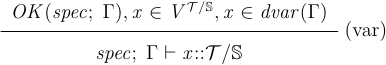
\includegraphics[scale=0.6]{Figures/zcga/1.png} \\
        \hline
        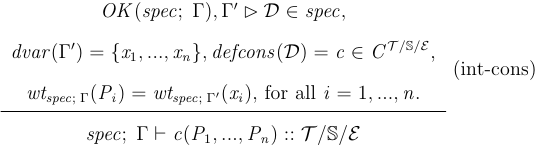
\includegraphics[scale=0.6]{Figures/zcga/2.png} \\
        \hline
        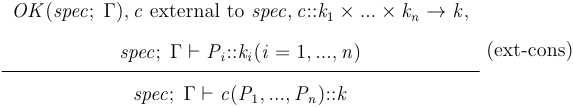
\includegraphics[scale=0.6]{Figures/zcga/3.png} \\
        \hline
        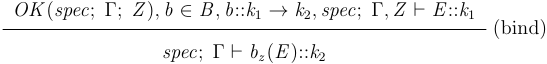
\includegraphics[scale=0.6]{Figures/zcga/4.png} \\
        \hline
        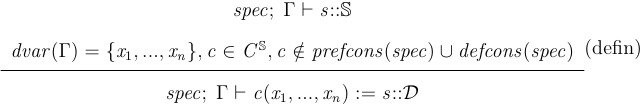
\includegraphics[scale=0.6]{Figures/zcga/5.png} \\
        \hline
        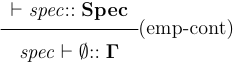
\includegraphics[scale=0.6]{Figures/zcga/6.png} \\
        \hline
        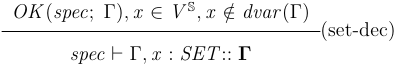
\includegraphics[scale=0.6]{Figures/zcga/7.png} \\
        \hline
        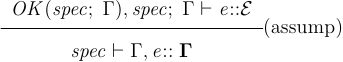
\includegraphics[scale=0.6]{Figures/zcga/8.png} \\
        \hline
        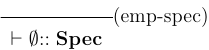
\includegraphics[scale=0.6]{Figures/zcga/9.png} \\
        \hline
        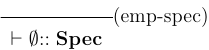
\includegraphics[scale=0.6]{Figures/zcga/10.png} \\
        \hline
    \end{tabular}
    \caption{Weak typing rules used by the ZCGa type checker. \label{tab:wttrules}}
\end{table}


%\begin{table}[H]
%\begin{tabular}{| c | c | } \hline 
%(var) & $\dfrac{OK(spec;\Gamma), x \in V^{\mathcal{T}/\mathbb{S}}, x \in
%dvar(\Gamma)}{spec;\Gamma \vdash x \mathbf{::}\mathcal{T}/\mathbb{S}}$
%\\[0.25cm] \hline
%(int-cons) & $\dfrac{\begin{aligned} OK(spec;\Gamma), \Gamma' \rres \mathcal{D}
%\in spec, \\[0.0001em]
%dvar(\Gamma')=\{x_{1}, ..., x_{n}\}, defcons(\mathcal{D}) = c \in
%C^{\mathcal{T}/\mathbb{S}/\mathcal{E}}, \\
%wt_{spec;\Gamma}(P_{i})=wt_{spec;\Gamma'}(x_{i}),\text{ for all }i = 1, ..., n
%\end{aligned}}% {spec;\Gamma \vdash c(P_{1}, ...,
%P_{n})::\mathcal{T}/\mathbb{S}/\mathcal{E}}$ \\[0.25cm] \hline
%(ext-cons) & $\dfrac{\begin{aligned} OK(spec;\Gamma), c \text{ external to
%spec}, c \mathbf{::} k_{1} \times... \times k_{n} \rightarrow k, \\
%spec;\Gamma \vdash P_{i} \mathbf{::} k_{i} (i=1,...,n) \end{aligned}}%
%{spec;\Gamma \vdash c(P_{1},...,P_{n}) \mathbf{::}k}$ \\[0.25cm] \hline
%(bind) & $\dfrac{OK(spec;\Gamma;Z), b \in B, b \mathbf{::}k_{1}\rightarrow
%k_{2}, spec;\Gamma, Z \vdash E \mathbf{::}k_{1}}{spec;\Gamma \vdash
%b_{z}(E)\mathbf{::}k_{2}}$ \\[0.25cm] \hline
%(defin)& $\dfrac{\begin{aligned} spec;\Gamma \vdash s \mathbf{::} \mathbb{S} \\
%dvar(\Gamma)=\{x_{1},...,x_{n}\}, c \in C^{\mathbb{S}}, c \notin prefcons(spec)
%\cup defcons(spec) \end{aligned}}% {spec;\Gamma \vdash c(x_{1},...,x_{n}):= s
%\mathbf{::} \mathcal{D}}$ \\[0.25cm] \hline
%& $\dfrac{\vdash spec \mathbf{:: Spec}}{spec \vdash \emptyset \mathbf{::
%\Gamma}}(emp-cont)$ \\[0.25cm] \hline
%(set-dec) & $\dfrac{OK(spec;\Gamma), x \in V^{\mathbb{S}}, x \notin
%dvar(\Gamma)}{spec \vdash \Gamma, x:SET \mathbf{:: \Gamma}}$ \\[0.25cm] \hline
%(term-dec) & $\dfrac{OK(spec;\Gamma), spec;\Gamma \vdash s \mathbf{::}
%\mathbb{S}, x \in V^{\mathcal{T}}, x \notin dvar(\Gamma)}{spec \vdash \Gamma,
%x:s \mathbf{:: \Gamma}}$ \\[0.25cm] \hline
%(assump) & $\dfrac{OK(spec;\Gamma), spec;\Gamma \vdash
%e\mathbf{::}\mathcal{E}}{spec \vdash \Gamma, e \mathbf{:: \Gamma}}$ \\[0.25cm]
%\hline
%(emp-spec) & $\dfrac{ }{\vdash \emptyset \mathbf{:: Spec}}$ \\[0.25cm] \hline
%(spec-ext) & $\dfrac{spec \vdash \Gamma \mathbf{:: \Gamma}}{\vdash spec, \Gamma
%\mathbf{:: Spec}}$ \\[0.25cm] \hline
%\end{tabular}
%\caption{Weak typing rules used by the ZCGa type checker. \label{tab:wttrules}}
%\end{table} 



\subsection{Weak typing properties and definitions}

Since the categories and rules of the Z syntax $WT_{Z}$ are a subset of the
original MathLang $WT_{M}$ \cite{wtt}, the following lemma holds:

\begin{lemma}
ZCGa properties \\

\begin{enumerate}
\item Types are unique. I.e.\ if $spec, \Gamma \vdash E \mathbf{::} W$ then $W$
is unique.

\item Type finding is decidable.\ I.e. for any $spec, \Gamma, E$, we can decide
if there is $W$/ $spec, \Gamma \vdash E \mathbf{::}W$.

\item Type checking is decidable. I.e. for $spec, \Gamma, E, W$ then we can
decide if $spec, \Gamma \vdash E \mathbf{::}W$.
\end{enumerate}
\end{lemma}



\subsection{Adapting weak types to the ZCGa}

For our \gls{zcga} checker we take the core categories from table
\ref{tab:wttrules}.

We use 7 categories, \textbf{Spec}, $\mathbf{\Gamma}$, $\mathcal{T}, \mathbb{S},
\mathcal{Z}, \mathcal{E}, \mathcal{D} $ corresponding to \textit{specification},
\textit{schematext}, \textit{term}, \textit{set}, \textit{declaration},
\textit{expression}, and \textit{definition} respectively. These categories and
weak typing rules will aid us to translate a specification into a full proof as
they help us complete the GPSa (see Figure \ref{fig:steps}).

\section{Annotations}

Using the ZMathLang \LaTeX{} package the user can label the specification with
\gls{zcga} annotations. This can be either before or after labelling the
specification with \gls{zdra} (see chapter \ref{ch:zdra}). The \gls{zcga}
annotations will highlight each individual grammatical aspect of the
specification. Table \ref{tab:zcgannot} shows how to label specifications with
\gls{zcga}.

\begin{table}[H]
\begin{tabular}{| l | l | l |}
\hline
\textbf{Category} & \textbf{\LaTeX{} label} & \textbf{Colour} \\
\hline
\hline
Specification & \verb|\specification{...}| & \specification{} \\
SchemaText & \verb|\text{...}| & \cgatext{} \\
Term & \verb|\term{...}| & \term{} \\
Set & \verb|\set{...}| & \set{} \\
Declaration & \verb|\declaration{...}| & \declaration{} \\
Expression & \verb|\expression{...}| & \expression{} \\
Definition & \verb|\definition{...}| & \definition{} \\
\hline
\end{tabular}
\caption{ZCGa \LaTeX{} annotations and their colours. \label{tab:zcgannot}}
\end{table}

\subsection{term}

According to the rules in table \ref{tab:wttrules} for an element to be a well
typed term it can be  a variable being declared such as \emph{t} (labelled in
blue) in figure \ref{fig:decinzcga} or it can be a constant giving a term. The
latter kind of term must have a constant within the preface of constants and a
variable which has been declared. An example of this could be the term
`\verb|#s|' (shown in figure \ref{fig:consterm}).

\begin{figure}[H]
\centering
\begin{tabular}{|c | c|}
\hline
\verb|\term{\# \set{s}}| & \term{\# \set{s}} \\
\hline
\end{tabular}
\caption{Constant giving a term \label{fig:consterm}}
\end{figure}

Figure \ref{fig:consterm} shows a constant giving a term. Provided that the set
\emph{s} is in the set of declared variable then the term \verb|# s| is a
correctly typed term.

\subsection{set}

Similar to typing a term, set can be correctly type in one of two ways. The
first is a variable set which is correctly declared such as `\emph{s}' in figure
\ref{fig:sdecinzcga}. The second way a set could be correctly typed is by having
a constant with parameters.

\begin{figure}[H]
\centering
\begin{tabular}{|c | c|}
\hline
\verb|\set{\set{s} \cup \set{s'}}| & \set{\set{s} \cup \set{s'}} \\
\hline
\end{tabular}
\caption{Constant giving a term \label{fig:consset}}
\end{figure}

Figure \ref{fig:consset} shows an example of a correctly typed set, consisting
of a constant and in this case two parameters (s and s'). So long as s and s'
are in the set of declared variables then `\emph{$s \cup s'$}' is a correctly
typed set.


\subsection{declaration}

There are two types of grammatically correct declaration:
\begin{enumerate}
\item term declaration
\item set declaration
\end{enumerate}

A term declaration is any declaration, expressing the relation between something
and it's type. For example if we had the declaration \verb|t: \nat| this is
declaring t is of type some sort of natural number. We can label this
declaration in \gls{zcga} (shown in figure \ref{fig:decinzcga})

\begin{figure}[H]
\centering
\begin{tabular}{|c | c|}
\hline
\verb|\declaration{\term{t}: \expression{\nat}}| & \declaration{\term{t}:
\expression{\nat}} \\
\hline
\end{tabular}
\caption{Correct term declaration labelled in zcga \label{fig:decinzcga}}
\end{figure}

We label \emph{$\nat$} as declarations for the same reasons as the typing's
behavior in \cite{wtt}.

The second type of declaration would be the declaration of a set, for example
\verb|s: \power \nat| this is saying that the set \emph{s} is in the set
\emph{$\power \nat$}. Figure \ref{fig:sdecinzcga} shows how this kind of
declaration would be labelled in \gls{zcga}

\begin{figure}[H]
\centering
\begin{tabular}{|c | c|}
\hline
\verb|\declaration{\set{s}: \expression{\power \nat}}| & \declaration{\set{s}:
\expression{\power \nat}} \\
\hline
\end{tabular}
\caption{Correct set declaration labelled in zcga \label{fig:sdecinzcga}}
\end{figure}

\subsection{expression}

An expression (named assump in the rules) is any correct expression within the
context. The expression can only contain correct sets and terms in the context.
Any constants within the expression must be in the preface of the \gls{zcga}
checker. A correct expression is shown in figure \ref{fig:expinzcga}.

\begin{figure}[H]
\centering
\begin{tabular}{|c | c|}
\hline
\verb|\expression{\term{t} \in \set{s}}| & \expression{\term{t} \in \set{s}}\\
\hline
\end{tabular}
\caption{Correct expression labelled in zcga \label{fig:expinzcga}}
\end{figure}

\subsection{definition}

If all the variables within the definition have been declared and the constant
the user is defining is a constant set. As well as the constant the user is
defining is not already in predefined and preface constants then the definition
is correct. A correct Z definition is shown in figure \ref{fig:definzcga}.

\begin{figure}[H]
\begin{footnotesize}
\centering
\begin{tabular}{|l|}
\hline
\verb|\definition{\LET \set{old} == \set{new} @ | \\
\verb|\expression{\term{t}\in\set{old}}}| 
\verb|\definition{\LET \set{old} == \set{new} @ | \\
\verb|\expression{\term{t} \in\set{old}}}| \\
\hline
\definition{\LET \set{old} == \set{new} @ \expression{\term{t} \in \set{old}}}\\
\hline
\end{tabular}
\end{footnotesize}
\caption{Correct definition labelled in zcga \label{fig:definzcga}}
\end{figure}

\subsection{schematext}

Schematext is all the correct declarations, expressions and definitions within a
specification. Figure \ref{fig:stinzcga} shows schematext which is correct. The
declaration and expression within the content of the schema would be classified
as schematext.

\begin{figure}[H]
\centering
\begin{minipage}{0.45\textwidth}
\begin{BVerbatim}
\begin{schema}{K}
\text{\declaration{\set{s}:
\expression{\power \nat}}}
\where
\text{\expression{\term{t} \in \set{s}}}
\end{schema}
\end{BVerbatim}
\end{minipage}\hfill
\begin{minipage}{0.45\textwidth}
\begin{schema}{K}
\cgatext{\declaration{\set{s}: \expression{\power \nat}} }
\where
\cgatext{\expression{\term{t} \in \set{s}}}
\end{schema}
\end{minipage}
\caption{Example of correct schematext \label{fig:stinzcga}}
\end{figure}

\subsection{specification}

Specifications are correct when the schematext is empty or all the schematext
within a specification is correct. A full example of a correctly labeled
specification in \gls{zcga} is shown in chapter \ref{ch:fullexample} in figure
\ref{fig:zcgaschemaout}.

\section{Implementation}

The \gls{zcga} program automatically checks the specification for grammatical
correctness. To do this it uses the \gls{zcga} annotations inputted by the user
and will notify the user if all is correct or any errors it may encounter. The
\gls{zcga} checker is a weak type checker. Therefore it only checks the
correctness of the weak types of the specification (annotated) and not actual Z
types like a Z type checker would find, such as fuzz.

\subsection{Checking if a specification is ZCGa correct}

The \gls{zcga} program uses regular expressions to read the annotations written
by the user to determine with a specification is \gls{zcga} correct. It ignores
all the parts which are not labelled in \gls{zcga} which allows for
\gls{semiform} to be checked as well. Look at the following:

\begin{exam}
\begin{verbatim}
There is a variable t which is a number that:
\text{\expression{\term{j} < \term{k}}}
\end{verbatim}
\end{exam}

This example shows a small specification that is \gls{semiform}, the \gls{zcga}
will read the annotations \verb|\text|, \verb|\expression| and \verb|\term|. It
will see that the specification contains a correct expression, however the
specification is \gls{zcga} incorrect as it would not pick up that the terms
have been declared. For this example to be \gls{zcga} correct the user will need
to change it into the example shown in \ref{Kexam}.

If the specification is correctly labelled and follows all the rules in table
\ref{tab:wttrules} then a message would appear saying \texttt{Spec Grammatically
Correct}. However if the specification is \gls{zcga} incorrect then a message
will appear saying `\texttt{Spec Grammatically Incorrect, Number of
errors:\emph{n}}' where \texttt{\emph{n}} will be a number with the number of
errors.

\begin{figure}[H]
\begin{tabular}{c c}
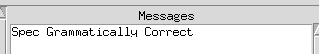
\includegraphics[width=7cm]{Figures/zcga/zcgacorrect.png} 
& 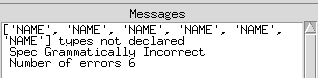
\includegraphics[width=7cm]{Figures/zcga/zcgaincorrect.png}
\end{tabular}
\caption{Message shown when specification is correct (left) and incorrect (right).\label{fig:correctandincorrect}}
\end{figure}

In figure \ref{fig:correctandincorrect} the left image shows the message when a
specification is \gls{zcga} correct. The right image shows a specification in
which a specification is not \gls{zcga} correct as the type `\texttt{NAME}' has
been used 6 times in the specification but has not been declared.

\subsection{Errors}
\label{subsec:zcgaerrors}

The specification is \gls{zcga} correct when all labelled objects within the
specification follow the \gls{zcga} type rules (table \ref{tab:wttrules}). Here
we highlight what error messages one might get when running the \gls{zcga}
checker on a specification.


\paragraph{\emph{term not declared}}

This follows the rules for variables in table \ref{tab:wttrules}. The message
`\emph{term not declared}' will appear if a term is labelled within the
schematext and there hasn't been a declaration defining its type previously.
Take a look at the following example fo a specification:

\begin{exam}
\label{Kexam}
\begin{verbatim}
\begin{schema}{K}
\text{\declaration{\term{j}:\expression{\nat}}}
\where
\text{\expression{\term{j} < \term{k}}}
\end{schema}
\end{verbatim}
\end{exam}

In the schematext containing the expression \verb|\term{j} < \term{k}| the term
\verb|j| has been previously declared with the type \verb|\nat| however the term
\verb|k| is labelled and used in the expression however it has not been declared
or assigned a type. This will cause the error message \emph{term not declared}.

\paragraph{\emph{set not declared}}

Similar to the previous error message, this follows the rules for variables in
table \ref{tab:wttrules}. The message \emph{set not declared} will appear when a
variable is labelled \verb|\set{..}| in the schematext of a specification but has
not been declared previously. Look at the following example:

\begin{exam}
\begin{verbatim}       
\begin{schema}{U}
\text{\declaration{\term{j}:\expression{\nat}}}
\where
\text{\expression{\term{j} \in \set{js}}}
\end{schema}
\end{verbatim}
\end{exam}

When the \gls{zcga} checker runs through this specification the error message
\emph{js: set not declared} should appear. This is because the term \verb|j| has
been declared, however the set \verb|js| has not been declared yet it is used in
the schematext \verb|\term{j} \in \set{js}|.

\paragraph{\emph{constant not in preface}}

When a constant is used within a specification that is not in the preface (see
\gls{zcga} code to see all constants in preface) then the `\emph{constant not in
preface}' error message will appear. An example is shown in the following
specification:

\begin{exam}
\begin{verbatim}       
\begin{schema}{T}
\text{\declaration{\set{t}:\expression{\mathbb{P} \nat}}}
\where
\text{\expression{\set{t} = \set{\{\}}}}
\end{schema}
\end{verbatim}
\end{exam}

The error message will appear here when running the \gls{zcga} checker on the
specification as the constant `\verb|\mathbb{P}|' is not in the preface. The
user in this case may have meant to use the constant \verb|\power| instead of
\verb|\mathbb{P}|. Even though these two constants look identical when compiling
a \LaTeX{} document they are not the same when checking specifications with
\gls{zcga}.

\paragraph{\emph{constant already in specification}}

The error message \emph{constant already in specification} will appear if the
user tries to define a constant which is already in the preface constants or
defined constants. For example take a look at the following specification:

\begin{exam}
\begin{verbatim}
\set{\nat} := \term{1} | \term{2} | \term{3} |...
\end{verbatim}
\end{exam}

The \gls{zcga} would say this specification is incorrect and the error
`\emph{constant already in specification}' would appear as the user is trying to
define the set of natural numbers \verb|\nat| however this constant is already
programmed in the preface of constants for Z specifications.

This error would also appear if the user tried to define a constant such as
\verb|[STUDENTS]| more  than once in their specification.

\paragraph{\emph{not a correct term}}

For this error message to appear, the user must have tried to create a term when
it wasn't allowed. Take the following example:

\begin{exam}
\begin{verbatim}       
\begin{schema}{Y}
\text{\declaration{\term{y}:\expression{\nat}}}
\where
\text{\expression{\term{\# \term{y}} = \term{0}}}
\end{schema}
\end{verbatim}
\end{exam}

This specification would be \gls{zcga} incorrect and the error message \emph{not
a correct term} would appear due to the term \verb|\term{\# \term{y}}| being
incorrect. This is because the constant \verb|\#| takes a set as a parameter and
gives back a term (the cardinality of the set). In this case the user has
applied a term \verb|\term{y}| to the constant \verb|\#| and thus the error
message appearing.

\paragraph{\emph{not a correct set}}

The error message \emph{not a correct set} will appear when a user has labelled
something as a set when it is not. For example take the following specification:

\begin{exam}
\begin{verbatim}       
\begin{schema}{W}
\text{\declaration{\term{w}:\expression{\power \nat}}}
\text{\declaration{\term{w'}:\expression{\power \nat}}}
\text{\declaration{\term{v}:\expression{\nat}}}
\where
\text{\expression{\set{w'} = \set{\set{w} \cup \term{v}}}}
\end{schema}
\end{verbatim}
\end{exam}

In this case the incorrect set would be \verb|\set{\set{w} \cup \term{v}}|. This
is because the constant \verb|\cup| takes two sets as parameters. However this
labelling shows that a set `\verb|w|' and a term `\verb|v|' have been applied. 

An example of a specification not passing the \gls{zcga} check is shown in
appendix \ref{app:nonworkingzcga}. This specification shows a telephone directory
which adds telephone numbers and names to a theoretical directory. It shows a
schema `\emph{TheTelephoneDirectory}' being used in the \emph{AddPerson}
schema, however `\emph{TheTelephoneDirectory}' is not a valid schema. The term
`\emph{person}' is being used in the `\emph{AlreadyInDirectory}' schema but only
the variable `\emph{persons}' has been declared. The term `\emph{numberInUse}'
is being used in the `\emph{NameNotInDirectory}' schema however the user might
of mistaken this term for the `\emph{nameNotInDirectory}' which has been
declared in the `\emph{OUTPUT}' freetype. The user has also forgotten the
variable decorations `\emph{?}' and `\emph{!}' on the `\emph{n}' and `\emph{s}'
variables in the `\emph{AddNumber}' schema.

All these errors may not be visible to the user when typing the specification or
looking at it with the naked eye, however with the user going through and
labelling each part in \gls{zcga} annotations along with the \gls{zcga} checker,
all these grammatical errors should be identified.

%If the user wished to ammend this then the set would change to
%\verb|\set{\set{w} \cup \set{\{\term{v}\}}}|. By adding the curly brackets
%\verb|\{..\}| it changes the term into a set which can now be applied as a
%parameter to \verb|\cup|.

\section{Benefits}

In addition to the main use for the \gls{zcga} checker which is to check the
grammar of a formal specification written in Z other \footnote{As a side note,
when copying specifications into this thesis I mistyped some words and they were
only caught when I ran the \gls{zcga} checker on them} benefits exists. The
\gls{zcga} would also be an advantage to the user or designer of a system to
translate their ideas to the developers of the system. For example by using the
\gls{zcga} the developers can clearly see which parts of the systems are
represented as sets and which parts are represented as terms. Not only does it
help describe the system to developers but other members of the project
development team and other stakeholders such as the client would also get a
better idea of the layout of the system. A further advantage to the \gls{zcga}
is that it is able to check the grammatical correctness of partially-formal
specifications. These can include specifications written in the english natural
language but are on their way to becoming formal, or specifications with formal
parts to them.

\section{ZCGa on a semiformal specification}

The \gls{zcga} can also be used on semiformal specification. An example is shown
in appendix \ref{app:semiform}, which describes an auto pilot system. This
specification is written partly in the english natural language and partly in Z.
Therefore the specification is on it's way to becoming formal. The user can then
annotate the formal parts and some of the informal parts in \gls{zcga}, it can
then be checked and will the user if there are any grammatical errors in the
specification so far, and if any variables which have been used need to be
declared etc. For example, in the auto pilot specification, the \verb|off_eng|
schema has a declaration which states \verb|mode:mode_status| (figure
\ref{fig:zcgautopilot}). If the \verb|mode_status| type was not declared before
it was used in the \verb|off_eng| schema, then the \gls{zcga} checker would
identify this and would display an error message. However, after the type
\verb|mode_status| has been declared in the specification it can be used
throughout the rest of the specification, including in the informal text part.

\begin{figure}[H]
\centering
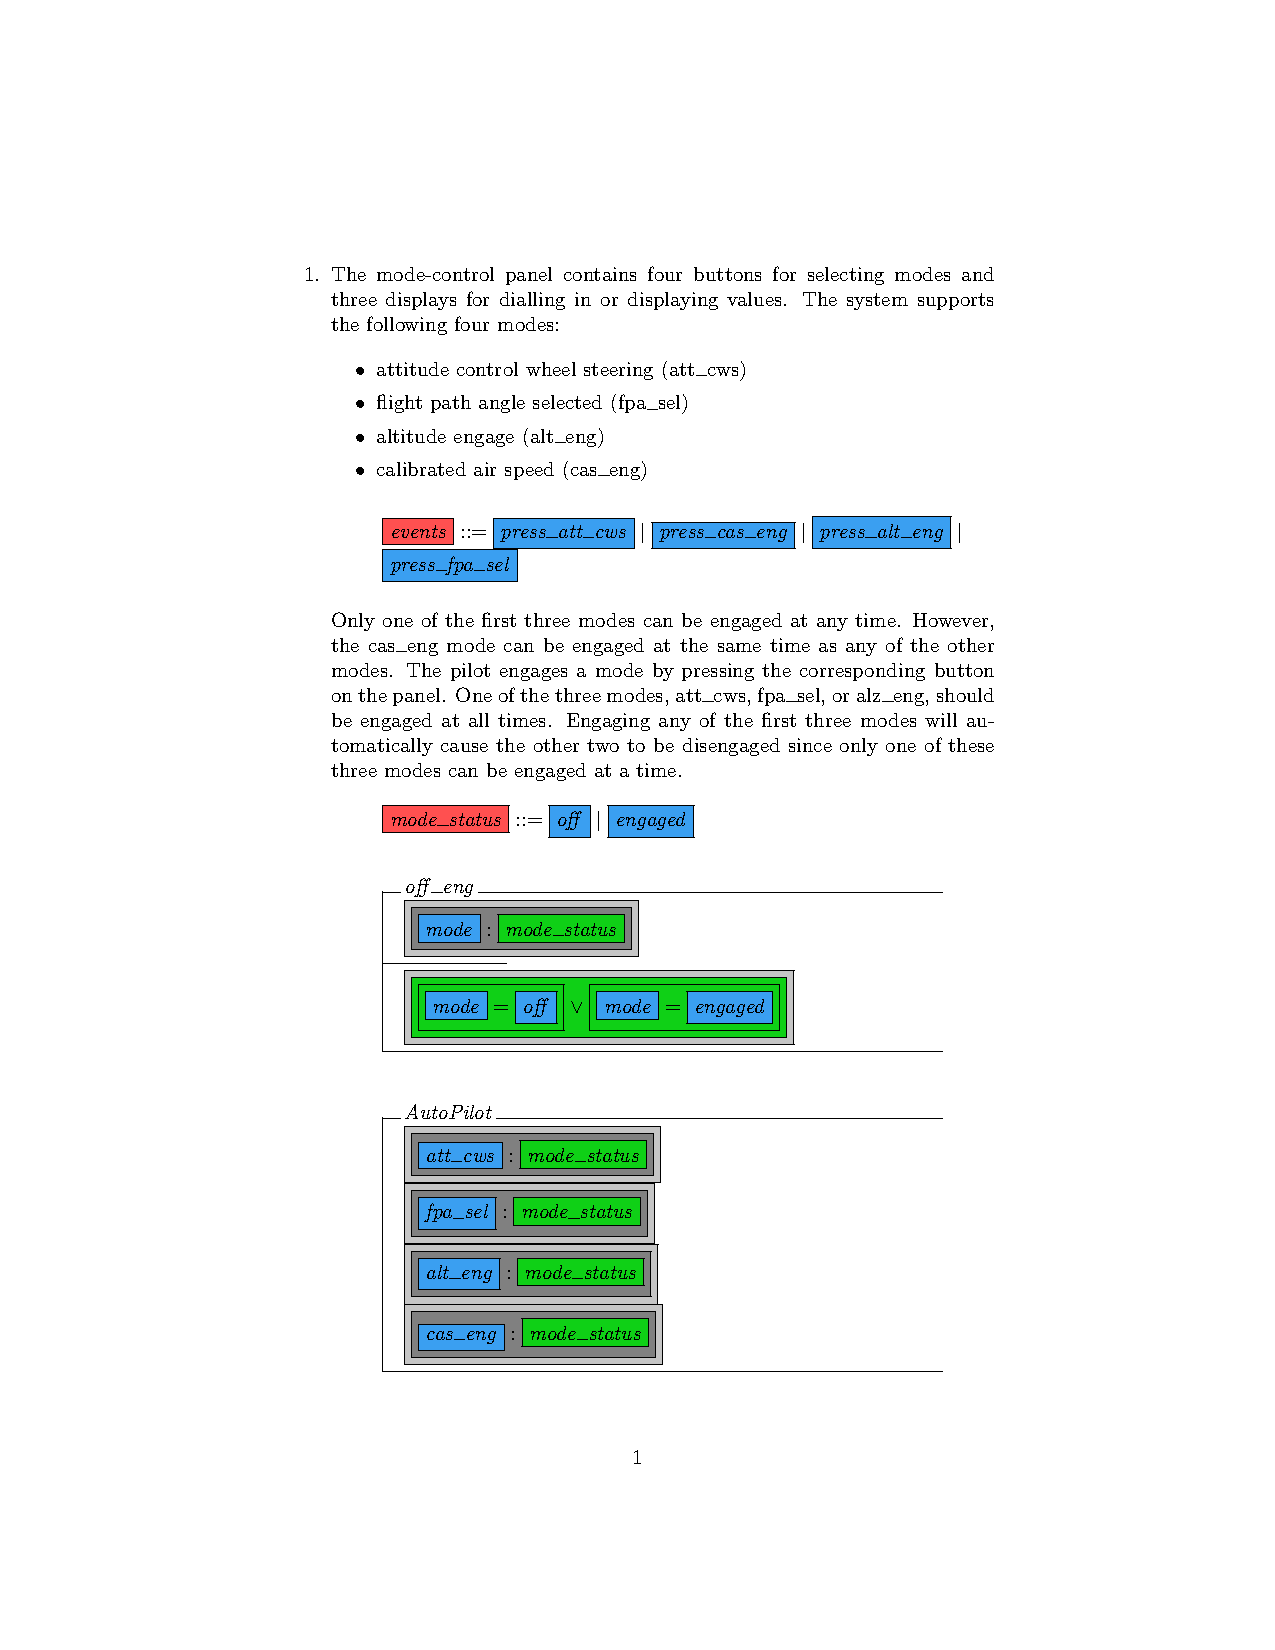
\includegraphics[clip, trim=3.5cm 10cm 1.5cm 2cm, scale=0.6]{examples/semiform/1.pdf}
\caption{Part of the Autopilot specification labelled in \gls{zcga}. \label{fig:zcgautopilot}}
\end{figure}

The full version of the semi formal specification is shown in appendix
\ref{app:zcgazdrasemiform}. Even though this specification is only partially
formal, we are able to translate the annotated parts all the way to the Isabelle
syntax (step 5 from figure \ref{fig:steps}).

\section{Conclusion}
In this chapter we have seen how the \gls{zcga} has grown from weak type theory
for mathematics \cite{wtt}. We have giving examples of different categories are
used within a Z specification and highlighted the rules these categories need to
follow in order to be \gls{zcga} correct. We have described a few properties of
the checker and have explained how these categories are transformed into weak
types for Z. We explained how a Z specification can be annotated and checked bu
the \gls{zcga} and given and illustrated the different errors which may arise.
The next step of the \gls{zmath} framework to check for another type of
correctness, the \gls{zdra}.

%\chapter{Z Document Rhetorical aspect}
\label{ch:zdra}
The \gls{zdra} is similar to the \gls{dra} for mathematics in MathLang. Here we describe how
the \gls{zdra} was designed an implemented. 

We use the ZMathLang \LaTeX{} package to chunk specifications together and see
the relationships between them. The mathematical instances used are
\textit{theory} and \textit{axiom}, which are used in theorem prover syntax. We
also use \textit{precondition}, \textit{postcondition}, \textit{output},
\textit{stateInvariants}, \textit{stateschema}, \textit{outputschema},
\textit{changeschema} and \textit{totaliseSchema}.

We created the ZDRa for the following:

\begin{itemize}

\item Identifying loops in the reasoning of specifications.
\item Checking the specification is robust by making sure schemas have been
totalised.
\item Identifying the relationships between chunks of specification.
\item Making sure state invariants do not change throughout the specification.
\item Creating a dependency graph to create a formal proof sketch from the ZDRa.
\end{itemize}

As well as having instances, the ZDRa shows relations between them to make sure
there are no loops in reasoning and to give warning in some situations (e.g.
specification is not totalised).

Identifying loops in the reasoning is important as it determines whether the
program is deterministic. Safety-critical systems must be deterministic,
practices which can lead to non-determinism must be avoided or carefully
controlled \cite{rierson2013developing}. Identifying loops in the reasoning is one of these practices. 

It is important to have a robust and totalised specification (in particular one
for a high integrity system) because totalisation leaves less room for error.
Specifications which are totalised are complete and therefore system
requirements are better understood and the programmer of the system would have
less assumptions about the system.
By totalising schemas all preconditions will have a corresponding postcondition.
Therefore when executing the system if all possible preconditions have a
corresponding output (post condition) then the computing system will be able to
handle errors better. Building a robust system encompasses as many points of
failure  as possible and one way to do this is to make the specification total.

Identifying relationships between chunks of specification is useful as it allows
us to carry out computations whether all dependencies are identified and to
check whether the relationships are sensible (for example all pre conditions
have a corresponding postconditions, a schema is defined if is used in another
schema). The relationships also allow users to explain the logical structure of
their system specification.

State invariants are conditions thats can be relied upon to be true during the
execution of the program. It is important that state invariants do not change as
they confirm your system specification is valid if the state invariants hold
even as the user states the preconditions and post conditions of each schema. 

The dependency graph is useful as it allows the user to identify which chunks of
specification are `\textit{dependent}' on each other i.e. if one chunk was
changed or removed then what other chunks would be affected. The dependency
graph also allow us to build the GoTo graph which in turn orders the
specification to be automatically written in a theorem prover.

Section \ref{sec:zdra_annotate} describes the labels used to annotate a
specification. Then in section \ref{sec:zdra_implement} we illustrate the
implementations of the \gls{zdra} and how to check for rhetorical correctness.
The rhetorical errors which can be found are explained in sections
\ref{subsubsec:zdra_looperrors} and \ref{subsubsec:zdra_toterrors} and the
products which are created when a specification is rhetorically correct are
described in section \ref{subsec:zdra_prodcuts}.

\section{Annotations}
\label{sec:zdra_annotate}

In a similar way as  MathLang for mathematics \ref{sec:mathlangbackground}, we can label the specifications with
\gls{zdra} annotations (either before of after the \gls{zcga}) using our ZMathLang \LaTeX{} package . These
annotations chunks parts of the specification together and upon compiling shows
the relationships between each of these chunks.

\begin{table}[H]
\begin{tabular}{| c | c | c | c |}
\hline
\textbf{Instance} & \textbf{Notation} & \textbf{\LaTeX{} Command}  \\
\hline
theory & T & $\backslash$dratheory\{\textit{T}\}\\
& & \{\textit{scaleoftheory}\}\{\textit{instance}\}  \\
\hline
stateschema & SS & $\backslash$draschema\{\textit{SS\#}\}\{\textit{instance}\}
\\
\hline
initschema & IS & $\backslash$draschema\{\textit{IS\#}\}\{\textit{instance}\}
\\
\hline
changeschema & CS & $\backslash$draschema\{\textit{CS\#}\}\{\textit{instance}\}
\\
\hline
outputschema & OS & $\backslash$draschema\{\textit{OS\#}\}\{\textit{instance}\}
\\
\hline
totaliseschema & TS &
$\backslash$draschema\{\textit{TS\#}\}\{\textit{instance}\}  \\
\hline
axiom & A  & $\backslash$draschema\{\textit{A\#}\}\{\textit{instance}\}  \\
\hline
stateInvariants & SI & $\backslash$draline\{\textit{SI\#}\}\{\textit{instance}\}
\\
\hline
precondition & PRE & $\backslash$draline\{\textit{PRE\#}\}\{\textit{instance}\}
\\
\hline
postcondition & PO  & $\backslash$draline\{\textit{PO\#}\}\{\textit{instance}\}
\\
\hline
output & O  & $\backslash$draline\{\textit{O\#}\}\{\textit{instance}\}  \\
\hline
\end{tabular}
\caption{\label{tab:instances} \gls{zdra} instances with their notations and \LaTeX{} commands.}
\end{table}

\begin{table}[H]
\begin{tabular}{| c | c |}
\hline
\textbf{Relation} &  \textbf{\LaTeX{} Command} \\
\hline
initialOf &  $\backslash$initialof
\{\textit{instance\_1}\}\{\textit{instance\_2}\}  \\
\hline
uses & $\backslash$uses \{\textit{instance\_1}\}\{\textit{instance\_2}\}\\
\hline
requires & $\backslash$requires
\{\textit{instance\_1}\}\{\textit{instance\_2}\}\\
\hline
allows & $\backslash$allows \{\textit{instance\_1}\}\{\textit{instance\_2}\}\\
\hline
totalises & $\backslash$totalises
\{\textit{instance\_1}\}\{\textit{instance\_2}\}\\
\hline
\end{tabular}
\caption{\label{tab:relations} \gls{zdra} Relations with their notations and \LaTeX{} commands.}
\end{table}

Table \ref{tab:instances} shows the type of instance available in a Z
specification, the notation that goes along with it and the \LaTeX{} command the
user annotates that part of the specification with. It is important to name
instances as these names are what are referred to when creating the
relationships between them. Table \ref{tab:relations} shows the relationships
which are available between some of the instances. 

The instances described in table \ref{tab:instances} are the building blocks of
what makes a Z specification. These large chunks of specification are what were
common across the literature describing Z specifications including Ed Curries descriptions \cite{essenceofz} and Spiveys descriptions
\cite{spiveyreferencemanual} in one form or another. Just like in MathLang for
mathematics \ref{sec:mathlangbackground} which included instances such as Lemma,
Theorem, Proof, Definitions we can group chunk of text together to identify what
is a theory, stateschema, initschema, changeschema, outputschema,
totaliseschema, axiom, stateInvariants, precondition, postcondition and output.

\subsection{Instances}

We have designed the notation to include \verb|\draschema{..}{..}| for chunks of
specification which include schemas and \verb|\draline{..}{..}| which only
include lines within a schema.

If we combine together \emph{changeschema} and \emph{outputschema} then these
instances are the minimum amount of labels we need to create a compilable
Isabelle file as both \emph{changeschema} and \emph{outputschema} become
`\emph{definitions}' in Isabelle. However we have decided to label
\emph{changeschema} and \emph{outputschema} separately as the user can easily
identify which schemas can change the state of the system and which just output
particular results.

\subsubsection{theory}

A \emph{theory} would be a whole specification of one particular system.
Appendix ?? shows an entire specification labelled in \gls{zdra}. You can have
more than one \emph{theory} in a single document. The \emph{theory} would
contain all other instances within it but no instance can have a \emph{theory}
inside of it.

\subsubsection{stateschema}

A \emph{stateschema} just like in Z is a single instance which outlines the
state of the system. Figure \ref{fig:exampleofss} shows an example of a
\emph{stateschema} instance. Note we have the label \verb|\draschema{SS1}{....}|
(shown in red) where we have labelled this \emph{stateschema} \verb|SS1|. There
may be one or more \emph{stateschema}'s in a theory. So users can label their
\emph{stateschema}'s accordingly, e.g.
\verb|SS1, SS2,SS3|.....\footnote{Although it is not needed for the user to annotate the
instances incrementally (the instances just need different names) we have used
it in our example to make it easier for the reader to identify how many of each instance is within the specification.}

\begin{figure}[H]
\centering
\begin{footnotesize}
\begin{BVerbatim}[commandchars=+\[\]]
[+color[red]\draschema{SS1}{]\begin{schema}{BirthdayBook}known: \power NAME \\
birthday: NAME \pfun DATE \where[+color[blue]\draline{SI1}{]known=\dom
birthday[+color[blue]}]\end{schema}[+color[red]}]
\end{BVerbatim}
\end{footnotesize}
\caption{\label{fig:exampleofss} A stateschema and stateinvariants labelled in \gls{zdra}.}
\end{figure}

\emph{Stateschema's} are important to identify as they go in the premuable of the
Isabelle file.

\subsubsection{initialschema}

An \emph{initialschema} instance is optional within a \emph{theory}, there can
be more than one depending on how many \emph{stateschema}'s there are. Figure
\ref{fig:exampleofis} shows an example of an \emph{initialschema}. We use the
labelling \verb|\draschema{IS1}{...}| (shown in red) to denote the
\emph{initialschema}. We have named the \emph{initialschema} \verb|IS1| to show
it is the first initial schema in the \emph{theory}. If there was another
\emph{initialschema} we would name it \verb|IS2| and so on.

\begin{figure}[H]
\centering
\begin{footnotesize}
\begin{BVerbatim}[commandchars=+\[\]]
[+color[red]\draschema{IS1}{]
\begin{schema}{InitBirthdayBook} 
BirthdayBook' 
\where 
[+color[blue]\draline{PO2}{]known' = \{ \}[+color[blue]}]
\end{schema}
[+color[red]}]
\end{BVerbatim}
\caption{\label{fig:exampleofis} An initialschema labelled in \gls{zdra}.}
\end{footnotesize}
\end{figure}

\emph{Initschema's} are important to identify as they become \emph{definitions}
Isabelle file (if it exists as they are not always defined in specifications).

\subsubsection{changeschema}

A \emph{changeschema} instance is a schema/function which changes the current
state of the specification (these schemas are usually denoted by having a
\verb|\Delta| operator). There can be none or many \emph{changeschema} instances
within a theory.

\begin{center}
\begin{figure}[H]
\centering
\begin{footnotesize}
\begin{BVerbatim}[commandchars=+\[\]]
[+color[red]\draschema{CS1}{]
\begin{schema}{AddBirthday}
\Delta BirthdayBook \\
name?: NAME \\
date?: DATE
\where
[+color[blue]\draline{PRE1}{]name? \notin known[+color[blue]}]
[+color[green]\draline{PO3}{]birthday' = birthday \cup \{name? \mapsto
date?\}[+color[green]}]
\end{schema}
[+color[red]}]
\end{BVerbatim}
\end{footnotesize}
\caption{\label{fig:exampleofcs} A changeschema labelled in \gls{zdra}.}
\end{figure}
\end{center}

Figure \ref{fig:exampleofcs} shows an example of a \emph{changeschema} annotated
in \gls{zdra}. The schema is labelled with: \verb|\draschema{CS1}{...}| (shown
in red). We name this instance \verb|CS1| as it is the first \emph{changeschema}
instance seen in the specification, the next \emph{changeschema} should be named
\verb|CS2| then \verb|CS3| etc.

\emph{Changeschema's} are important to identify as they become \emph{definitions}
Isabelle file (if it exists as they are not always defined in specifications).

\subsubsection{outputschema}

An \emph{outputschema} instance is a schema or a function which does not change
the current state but only outputs information from the current state (these
schemas are usually denoted by having a \verb|\Xi| operator). Figure
\ref{fig:exampleofos} shows an example of an \emph{outputschema} instance in
\gls{zdra}. Note the line \verb|\draschema{OS4}{....| (shown in red) which names
the chunk \verb|OS4| that is the forth \emph{outputschema} in the specification.

\begin{figure}[H]
\centering
\begin{footnotesize}
\begin{BVerbatim}[commandchars=+\[\]]
[+color[red]\draschema{OS4}{]
\begin{schema}{AlreadyKnown}
\Xi BirthdayBook \\
name?: NAME \\
result!: REPORT
\where
[+color[blue]\draline{PRE3}{]name? \in known[+color[blue]}] \\
[+color[green]\draline{O4}{]result! = already\_known[+color[green]}]
\end{schema}
[+color[red]}]
\end{BVerbatim}
\end{footnotesize}
\caption{\label{fig:exampleofos} A outputschema labelled in \gls{zdra}.}
\end{figure}

\emph{Outputschema's} are important to identify as they become \emph{definitions}
Isabelle file (if it exists as they are not always defined in specifications).

\subsubsection{totaliseSchema}

\emph{Totaliseschema} instances are parts of the specification which totalise
preconditions within the specification. These are labelled as
\verb|TS#| where \verb|#| is some number. \emph{Totaliseschema} instances can written
in two ways. Either using the double equals operator:

\begin{verbatim}
\begin{zed}
A == B \land C
\end{zed}
\end{verbatim}

or by using the \verb|defs operator|:

\begin{verbatim}
\begin{zed}
A \defs B \land C
\end{zed}
\end{verbatim}

When labelling \emph{totaliseschema} instances the user can do this in two ways. The
first labelling is as a \verb|draschema| where the labelling comes before the
\verb|\begin{zed}| or as a \verb|draline| where the labelling wraps around the
line of the instance only. The second way is useful if there are more than one
\emph{totaliseschema} instance between the \verb|\begin{zed}| and \verb|\end{zed}|. 

\begin{figure}[H]
\centering
\begin{footnotesize}
\begin{BVerbatim}[commandchars=+\[\]]
[+color[red]\draschema{TS3}{]
\begin{zed}
VM3 \defs VM1 \lor VM2 \end{zed}[+color[red]}]
\end{BVerbatim}
\end{footnotesize}
\caption{\label{fig:exampleofts1} A totalise schema instance labelled in \gls{zdra}.}
\end{figure}

An example of the \verb|draschema| labelling is shown in figure
\ref{fig:exampleofts1} where we have the label \verb|\draschema{TS3}{..| (shown
in red).

\begin{figure}[H]
\centering
\begin{footnotesize}
\begin{BVerbatim}[commandchars=+\[\]]
\begin{zed} 
[+color[red]\draline{TS1}{]RAddBirthday == (AddBirthday \land Success)\\  \lor
AlreadyKnown[+color[red]}] \\
[+color[red]\draline{TS2}{]RFindBirthday == (FindBirthday \land Success) \lor
NotKnown[+color[red]}] \\
[+color[red]\draline{TS3}{]RRemind == Remind \land Success[+color[red]}]
\end{zed}
\end{BVerbatim}
\end{footnotesize}
\caption{\label{fig:exampleofts2} A totalise line instance labelled in \gls{zdra}.}
\end{figure}

An example of the \verb|draline| instance is shown in figure \ref{fig:exampleofts2}. In this example we have three \emph{totalise instances}
using the label \verb|\draline{TS1}{...|, \verb|\draline{TS2}{...| and
\verb|\draline{TS3}{...| respectfully (shown in red).

\emph{Totaliseschema} instances become the properties to prove when converted to the
half-baked proof (see chapter \ref{ch:skeletons} for details). This is because
totaliseschema instances will should contain a preconditions and postconditions
which should obey they stateinvariants within the specification. Totaliseschema
instances should be total and therefore complete. If all the totaliseschemas are
proved correct then their should be less room for errors within the entire
system.

\subsubsection{axiom}

\emph{Axiom} instances are knowns as axiomatic definitions in Z. There can be
more than one \emph{axiom} in a \emph{theory} or there can be none. An example
of an \emph{axiom} instance labelled in \gls{zdra} is shown in figure
\ref{fig:exampleofa}. Note the \gls{zdra} labelling consists if the line
\verb|\draschema{A1}{...| where the instance is named \verb|A1|.

\begin{figure}[H]
\centering
\begin{footnotesize}
\begin{BVerbatim}[commandchars=+\[\]]
[+color[red]\draschema{A1}{]
\begin{axdef}
maxPlayers: \nat
\where
maxPlayers = 20 \end{axdef}[+color[red]}]
\end{BVerbatim}
\end{footnotesize}
\caption{\label{fig:exampleofa} A axiom instance labelled in \gls{zdra}.}
\end{figure}

\emph{Axioms} are important to identify as they go in the premuable of the
Isabelle file.

\subsubsection{stateInvariants}
The \emph{stateInvariants} instance are the conditions which must be obeyed
throughout the specifications. These are the lines founds inside the
\emph{stateschema} instance. Figure \ref{fig:exampleofss} shows a single
\emph{stateinvariant} instance labelled as \verb|\draline{SI1}{..| (shown in
blue). There can be 0 or more \emph{stateinvariance} instances within a
\emph{theory}. \emph{StateInvariants} are important to be identified in the ZDRa
as they come after the `\emph{assumes}' in the isabelle syntax (see chapter
\ref{chap:gpsa2isa} to see how stateinvariants are translated). Each definition
and lemma then described in Isabelle makes sure that all conditions obey the stateinvariants.

\subsubsection{precondition}

Similar to the \emph{totalise} instance, the \emph{precondition} instance can be
labelled as a \verb|draschema| or a \verb|draline|. An example of a
\emph{precondition} which is a line can be found in figures
\ref{fig:exampleofcs} and \ref{fig:exampleofos}. In figure \ref{fig:exampleofcs}
the \gls{dra} labelling for a \emph{precondition} schema is the line
\verb|\draline{PRE1}{..}| (shown in blue). The \emph{precondition} instance is
named \verb|PRE1| and \verb|name? \notin known| is the instance. In figure
\ref{fig:exampleofos} the \gls{zdra} labelling is 
\verb|\draline{PRE3}{..}|(shown in blue) where \verb|PRE3| is the name of the
instance and 
\verb|name?\in known| is the instance.

Another way a \emph{precondition} instance can exists is when an entire schema
only consist of \emph{precondition} instances and nothing else (no post
operations).

\begin{figure}[H]
\centering
\begin{footnotesize}
\begin{BVerbatim}[commandchars=+\[\]]
[+color[red]\draschema{PRE1}{]
\begin{schema}{exact\_cash}
cash\_tendered?: \nat
\where
cash\_tendered? = price \end{schema}[+color[red]}]
\end{BVerbatim}
\end{footnotesize}
\caption{\label{fig:exampleofpre} A precondition schema instance labelled in \gls{zdra}.}
\end{figure}

A \emph{precondition} instance which is an entire schema is shown in figure
\ref{fig:exampleofpre}. The \gls{zdra} labelling consists of the line
\verb|\draschema{PRE1}{..| where the name of the instance is \verb|PRE1|.

\emph{Precondition's} are important to identify as they must be checked that they
conform with the stateInvariants of the specification.

\subsubsection{postcondition}

The \emph{postcondition} instance can be labelled as a \gls{zdra} line. An
example of this is demonstrated in figure \ref{fig:exampleofcs} (shown in
green), where the name of the instance is \verb|PO3| and the instance itself is
\verb|birthday' = birthday \cup \{name? \mapsto date?\}|.

\emph{Postconditions's} are important to identify as they must be checked that they
conform with the stateInvariants of the specification.

\subsubsection{output}

An \emph{output} instance can also be labelled as a \gls{zdra} line. An example
of this is shown in green in figure \ref{fig:exampleofos}. The instance in this
case is named
 \verb|O4| and the instance itself is \verb|result! =already\_known|.

 \emph{Output's} are important to identify as they must be checked that they
conform with the stateInvariants of the specification.
\subsection{Relations}
\label{subsec:zdrarelations}

After labelling the instances within a relation the user may then add relations
between parts of the specification. The relationships available are
\emph{initialOf}, \emph{uses}, \emph{requires} and \emph{allows}.

\begin{table}[H]
\begin{tabular}{|lll||lll|}
\hline
\textbf{requires} & & &  & \textbf{uses} & \\
\hline
outputSchema & $\longrightarrow$ & precondition  & outputSchema &
$\longrightarrow$ & stateSchema\\
outputSchema & $\longrightarrow$ & output & changeSchema & $\longrightarrow$ &
stateSchema \\
changeSchema & $\longrightarrow$ & precondition  & stateSchema &
$\longrightarrow$ & stateSchema \\
changeSchema & $\longrightarrow$ & postcondition  & stateSchema &
$\longrightarrow$ & axiom \\
\cline{1-3}
\textbf{totalises} & &  & outputSchema & $\longrightarrow$ & axiom \\
\cline{1-3}
totaliseschema & $\longrightarrow$ & changeSchema  & changeSchema & $\longrightarrow$
& axiom \\
\cline{4-6}
totaliseschema & $\longrightarrow$ & outputSchema & \textbf{allows}  & & \\
\cline{4-6}
totaliseschema & $\longrightarrow$ & totaliseschema  & precondition  & $\longrightarrow$  &
postcondition \\
\cline{4-6}
totaliseschema & $\longrightarrow$ & precondition & \textbf{initialOf} &  &  \\ 
\cline{4-6}
& &  & initialSchema & $\longrightarrow$ & stateSchema \\ 
\hline
\end{tabular}
\caption{\label{tab:relationsallowed} The legal relations between instances. Where $\longrightarrow$ represents the relation.}
\end{table}

Table \ref{tab:relationsallowed} shows the legal relations between each of the
instances for example an \emph{initialSchema} can be an \emph{initialOf} a
\emph{stateSchema} but it wont allow say a \emph{changeSchema} to be
\emph{initialOf} an \emph{initialSchema} etc. These relations are all we need to
create a Dependency and GoTo graph and to describe the relationships between the
instances of the specification. These relations are also the minimum we need to
create the program to automatically translate the specification in the correct
order into an Isabelle file.

\subsubsection{initialOf}

An \emph{initialschema} instance can be an \emph{initialOf} a \emph{stateschema}
instance. An example of this would be \verb|\initialOf{IS1}{SS1}| where
\verb|IS1| is \emph{initialOf} \verb|SS1|.

\subsubsection{uses}
The \emph{uses} relation can be between \emph{changeSchema}'s,
\emph{outputSchema}'s, \emph{stateSchema}'s and \emph{totalise} instances. For
example, one can say that an \emph{outputSchema} \emph{uses} a
\emph{stateSchema}. To illustrate this the user can add the label
\verb|\uses{OS2}{SS1}|, meaning \emph{outputSchema} OS2, uses \emph{stateSchema}
SS1.

\subsubsection{requires}
The \emph{requires} relation is used between an \emph{outputSchema} or a
\emph{changeSchema} and a \emph{precondition}, \emph{output} or
\emph{postcondition}. If we take the example shown in figure
\ref{fig:exampleofis} we can say that the \emph{initialSchema} \verb|IS1|
\emph{requires} the postcondition \verb|PO2|. Therefore in \gls{zdra} notation
we would write in our \LaTeX{} specification \verb|\requires{IS1}{PO2}|.

\subsubsection{allows}
The \emph{allows} relation is used between \emph{precondition}'s and
\emph{postconditions} or \emph{preconditions} and \emph{outputs}. This relation
describes if an instance allows another instance to occur. That is an instance
can not exist unless pre-conditional requirements are met. An example of where
an \emph{allows} relationship would be useful is in figure
\ref{fig:exampleofos}, where we have a \emph{precondition} \verb|PRE3| (in blue)
and an \emph{output} \verb|O4| (in green). In this case the user would write in
their \gls{zdra} \LaTeX{} file: \verb|\allows{PRE3}{O4}|.

\subsubsection{totalises}
The \emph{totalise} relation allows users to describe which of their schema's
have been totalised. If there exists a precondition which has not been totalised
than the ZDRa check will identify this (see next section). Any schema which
contains \emph{preconditions} be totalised in a \emph{totaliseschema}. For
example the the user can label \verb|\totalises{TS1}{PRE1}|


\section{Implementation}
\label{sec:zdra_implement}

The \gls{zdra} program automatically checks for rhetorical correctness of the
specification. To do this it reads the \gls{zdra} annotations created by the
user then if all is correct then the program automatically generates a
\emph{dependency graph} and a \emph{goto graph}. The input for the \gls{zdra}
program is the specification written in \LaTeX{} with the \gls{zdra}
annotations.

\subsection{Checking if a specification is correctly totalised}
\label{subsec:correctlytotalised}

The \gls{zdra} program uses regular expressions to read the annotations inputted
by the user to determine whether a specification has been totalised. For example
if we only have a single \emph{precondition} instance (PRE1), in a specification
and a single \emph{totalise} instance (TS1), in a specification and the user has
added the \emph{relation} \verb|totalises{TS1}{PRE1}|, then the specification
will be correctly totalised and there will be a message saying
"\texttt{Specification correctly totalised}". If there exists any preconditions
which the user hasn't annotated with a totalising relation then the \gls{zdra}
program will display a message saying "\texttt{Specification not correctly
totalised}". This message is a warning not an error therefore even if the
specification still has untotalised preconditions the user can still go on with
the next steps of computerisation.

It is important to have correctly totalised specifications, especially in safety
critical systems as it leaves less room for error when translating specification
into actual programs. If every preconditions have a corresponding postcondition
than the specification will be deemed `\emph{totalised}' and therefore a safer
system. With a totalised specification the programmer would not need to make any
assumptions and any defined state the system is in will have a corresponding
postcondition. Totalisation also adds a level of rigour to the specification for
example in the Sholis project \cite{sholis} described in chapter
\ref{ch:background} the Z specification found 75\% of faults in the system.
Without a totalised specification those faults would of been implemented in the
system and then potentially only found during testing where a lot of time and
money would of been spent.

\subsubsection{Errors}
\label{subsubsec:zdra_toterrors}

Table \ref{tab:totalisecorrect} shows examples of 3 specifications (named 1, 2
and 3). Specification 1 shows three \emph{preconditions} being annotated by the
user (PRE1, PRE2 and PRE3), all these preconditions have been annotated with the
relationship \emph{totalises}. Therefore if all preconditions in a schema have a
totalising condition then the specification is correctly totalised.
Specification 2 in the table shows 4 existing preconditions. All but one (PRE2)
precondition have a totalising relationship with a totalise schema. In this
case, PRE2 is an outstanding preconditions to be totalised and therefore the
message `\texttt{Specification incorrectly totalised} appears. Specification 3 in
table \ref{tab:totalisecorrect} shows 5 schema preconditions. When checking
totalising correctness it does not matter whether the preconditions are in
\verb|draline| form or \verb|draschema| form. In the third example we see that
PRE3 and PRE4 have not been totalised and again a message appears saying the
specification has not been correctly totalised.

\begin{table}[H]
\begin{tabular}{|c|c|c|c|}
\hline
& \textbf{Preconditions in} & \textbf{Totalises in} & \textbf{Outcome of} \\
& \textbf{specification} & \textbf{specification} & \textbf{\gls{zdra} program}
\\
\hline
\hline
& \verb|\draline{PRE1}| & \verb|\totalises{TS1}{PRE1}| & \\
1 & \verb|\draline{PRE2}| & \verb|\totalises{TS1}{PRE2}| & `\texttt{Spec
correctly} \\
& \verb|\draline{PRE3}| & \verb|\totalises{TS2}{PRE3}|& \texttt{totalised}'\\
\hline
& \verb|\draline{PRE1}| & \verb|\totalises{TS1}{PRE1}| &  \\
2 & \verb|\draline{PRE2}| & & \\
& \verb|\draline{PRE3}| & \verb|\totalises{TS2}{PRE3}|& `\texttt{Spec
incorrectly} \\
& \verb|\draline{PRE4}| & \verb|\totalises{TS3}{PRE4}|& \texttt{totalised}' \\
\hline
& \verb|\draschema{PRE1}| & \verb|\totalises{TS1}{PRE1}| &  \\
 & \verb|\draschema{PRE2}| & \verb|\totalises{TS2}{PRE2}| & \\
3 & \verb|\draschema{PRE3}| & & `\texttt{Spec incorrectly} \\
& \verb|\draschema{PRE4}| &  & \texttt{totalised}' \\
& \verb|\draschema{PRE5}| & \verb|\totalises{TS2}{PRE5}|  & \\
\hline
\end{tabular}
\caption{\label{tab:totalisecorrect} Examples of preconditions in a specification being correctly totalised and incorrectly totalised.}
\end{table}

\subsection{Checking if a specification has no loops in it's reasoning}
\label{subsec:loops}

The \gls{zdra} program also checks for rhetorical correctness, that is it checks
that there are no loops in the logical reasoning of the specification. To do
this the \gls{zdra} program imports a module named \texttt{networkX} to create a
\emph{directed graph}. The program also uses \emph{regular expressions} to read
the \gls{zdra} annotations and create nodes and edges. For example, if the
program finds \verb|\draline{x}{....}| or \verb|draline{y}{...}| then it will
add \texttt{x} and \texttt{y} as nodes to the directed graph. The edges are
created by reading the \emph{relations} in the \gls{zdra} annotated
specification. For example if the \gls{zdra} program finds \verb|\uses{x}{y}|
and \texttt{x} and \texttt{y} are nodes in the directed graph then it will add a
directed edge between \texttt{x} and \texttt{y} respectively. Nodes with no
edges at all can also be added to the graph.

Loops in the reasoning identify when two specifications or functions can call
one another (mutual recursion). This should be avoided when writing safety critical systems because
a system which has mutual recursion could possibly overload the stack and the
software will crash.

\subsubsection{Errors}
\label{subsubsec:zdra_looperrors}

The specification is correct when there are no loops in the created directed
graph. For example if there was a graph with edges [a$\rightarrow$b,
a$\rightarrow$c, b$\rightarrow$c] then that would still be legal as there are no
directed loops, however, if there was a graph with edges [a$\rightarrow$b,
b$\rightarrow$c, c$\rightarrow$a] then that would cause a loop in the reasoning
and the specification will not be \gls{zdra} correct. The program outputs a
message informing the user whether the specification is \gls{zdra} correct or
not.

\begin{figure}[H]
\vspace{-0.2in}
\centering
\begin{minipage}{0.45\textwidth}
\centering
\begin{scriptsize}
\begin{BVerbatim}
... \draschema{SS1}{
\begin{schema}{A}
C
\end{schema}}
\draschema{SS2}{
\begin{schema}{B}
A
\end{schema}}
\draschema{SS3}{
\begin{schema}{C}
B
\end{schema}}

\uses{SS1}{SS3}
\uses{SS2}{SS1}
\uses{SS3}{SS2}
...
\end{BVerbatim}
\end{scriptsize}
\vspace{-0.18in}
\caption{An example of a loop in the reasoning in a labelled ZDRa specification.\label{fig:aloop}}
\vspace{-0.2in}
\end{minipage}\hfill
\begin{minipage}{0.45\textwidth}
\centering
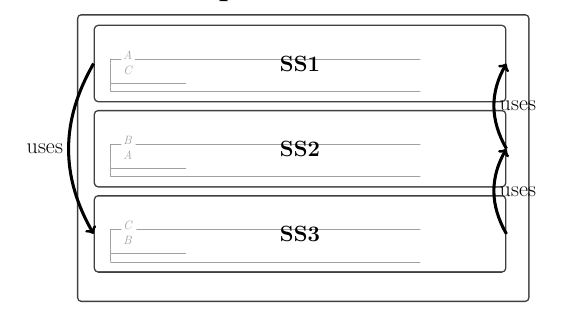
\includegraphics[scale=0.33]{Figures/zdra/zdraloop.png}
\vspace{-0.18in}
\caption{The pdflatex output of figure \ref{fig:aloop}.  \label{fig:zdraerror1}}
\vspace{-0.2in}
\end{minipage}
\end{figure}

Figure \ref{fig:zdraerror1} shows the relationship SS1 \textit{uses} SS3, SS2
\textit{uses} SS1 and SS3 \textit{uses} SS2. The ZDRa would not allow this as
the reasoning would be in a loop and would not be correct. When running the
\gls{zdra} check on this specification the message which would appear is shown
in figure \ref{fig:zdraerrormess}

\begin{figure}[H]
\centering

\includegraphics[scale=0.5]{Figures/zdra/loopmessage.png}
\caption{An example of an error message when a specification is not \gls{zdra} correct. \label{fig:zdraerrormess}}
\end{figure}

If the specification is \gls{zdra} correct then the program also creates visual
dependency and GoTo graphs automatically (see section
\ref{subsec:zdra_prodcuts}). If not then the graphs are not created.

A full specification which passes \gls{zcga} is shown in appendix
\ref{app:failzdra}. There is one loop in the reasoning of this specification and
the user is able to see it when they annotated the specification in \gls{zdra}
and have compiled the document using \texttt{pdflatex}. A snippet of this is
shown in figure \ref{fig:zdraloopsnippet} and the full version is shown in
appendix \ref{app:failzdraout}.

\begin{figure}[H]
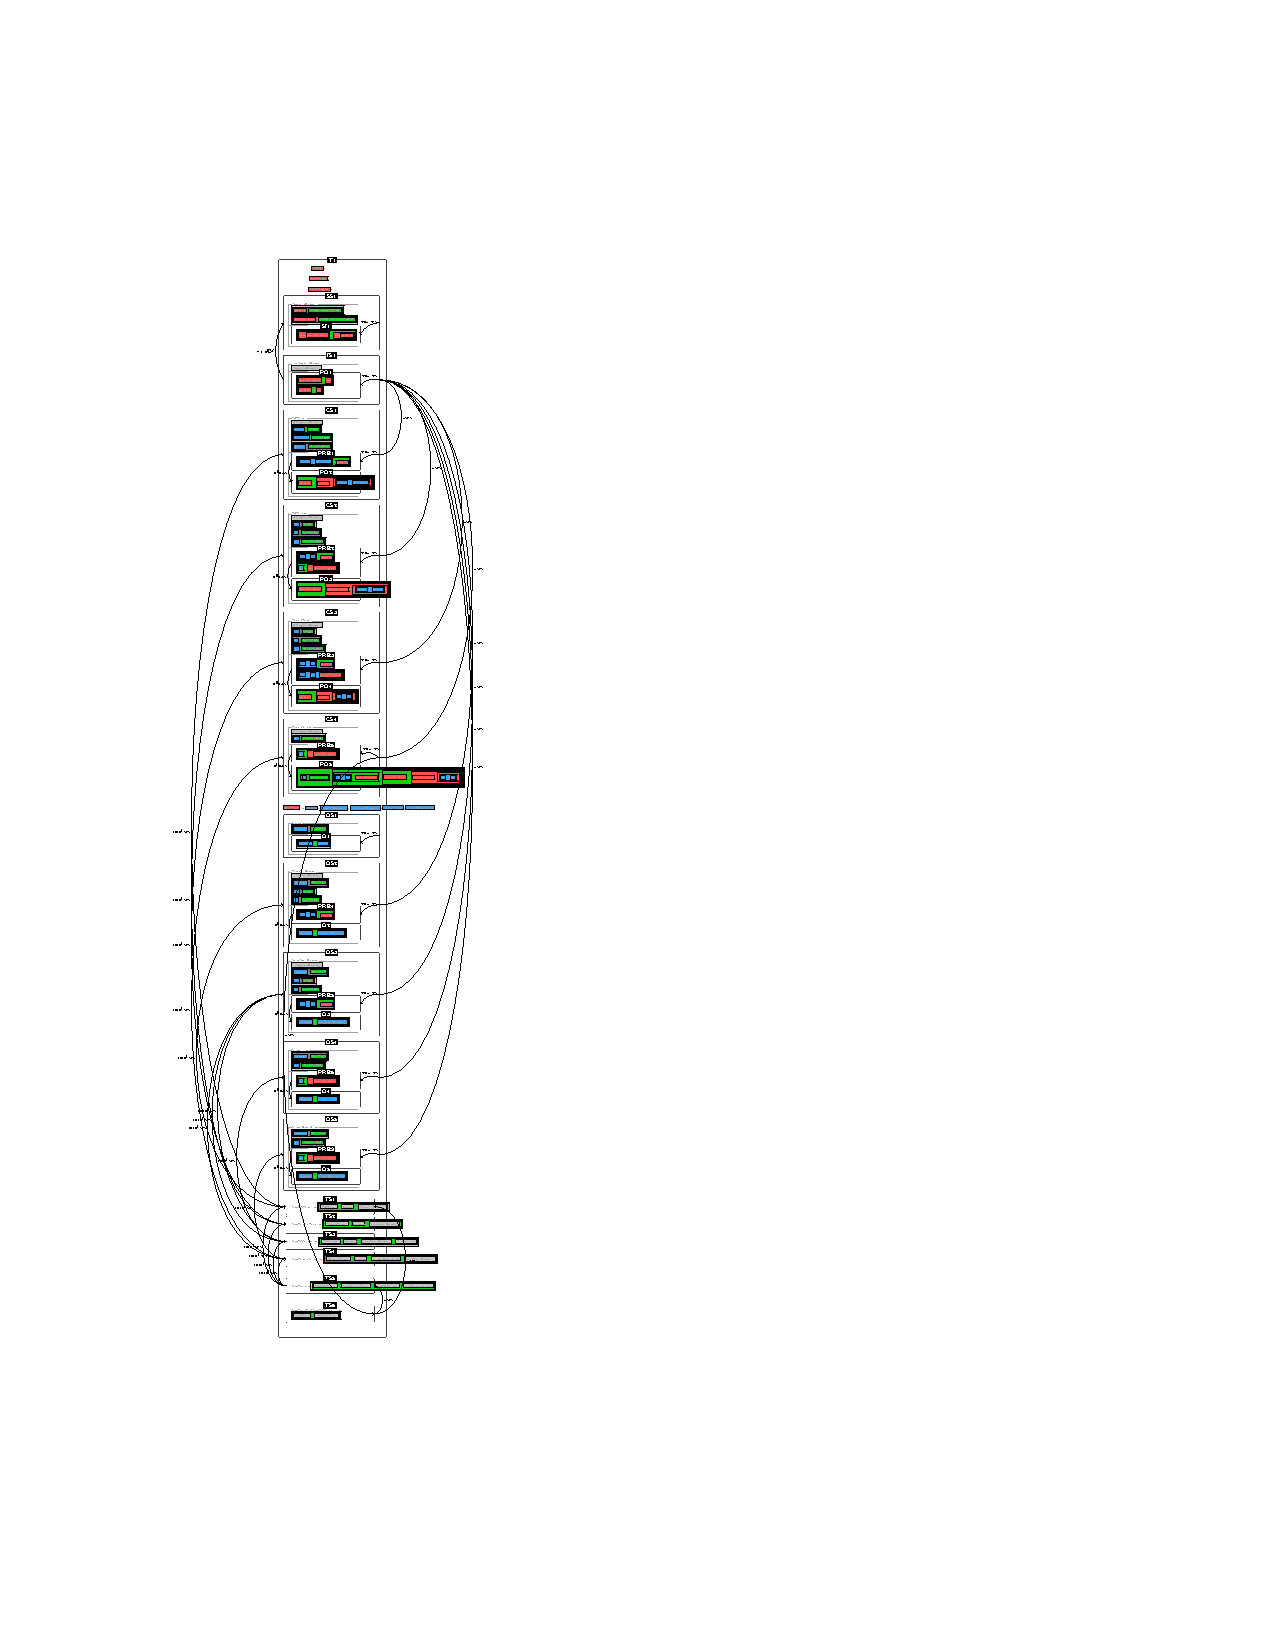
\includegraphics[clip, trim=0cm 10cm 6cm 11cm, scale=1.3]{examples/nonworkzdra/1n2.pdf}
\caption{A snippet from appendix \ref{app:failzdra} showing a loop in reasoning. \label{fig:zdraloopsnippet}}
\end{figure}

When the specification is checked with \gls{zcga} then the output message says
the specification is grammatically correct. However when the specification is
checked with \gls{zdra}, the message says that circular reasoning has been found
and shows the path of the loop, which in this case is \verb|CS4, TS4, TS5, TS6|.
The error message which appears specifically for this example in shown in figure
\ref{app:failzdraoutmessgae} in appendix \ref{app:failzdraoutmes}.

\subsection{ZDRa Outputs}
\label{subsec:zdra_prodcuts}

When the specification has been ZDRa checked the program will then output two
new files. 

\begin{enumerate}

\item ZDRa specification Dependency Graph

\item ZDRa specification GoTo Graph
\end{enumerate}

The \gls{zdra} specification Dependency graph uses the labels and annotations
from the \gls{zdra} to show the dependencies between each of the instances. The
ZDRa GoTo graph illustrates which instances are dependent or are needed for
another instance to exist. Both graphs are built using the directed graph built
in the \gls{zdra} check (see section \ref{subsec:loops}). Further information on
how these products are formed can be found in the next chapter.

\subsubsection{Dependency Graph}

\begin{figure}[H]
\centering
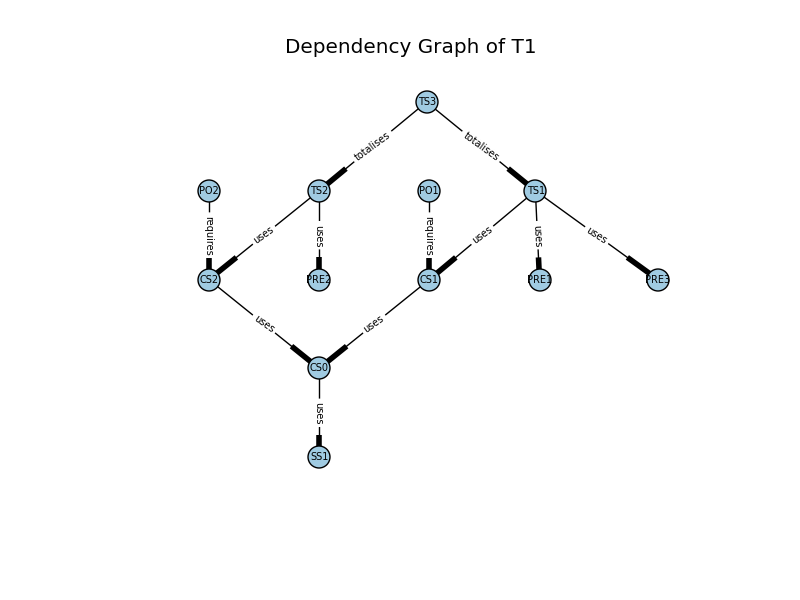
\includegraphics[scale=0.6]{Figures/zdra/depgraph.png}
\caption{An example of a dependency graph. \label{fig:depgraph}}
\end{figure}

An example of a \emph{dependency graph} can be seen in figure
\ref{fig:depgraph}. This image represents the compiled \gls{zdra} annotated
document but it graph form. All the boxes that show up in the compiled document
are represented by nodes in the graph. The arrows from the instances are
represented by the edges in the graph, all the arrows in the document and edges
in the graph should be pointing in the same direction.

The dependency graph is a directed graph representing dependencies
of several towards one another. The benefits of a dependency graph would be for system analysis, one can see
which parts of the specification are \textbf{dependent} on others. For example
if one were to change a function (schema) which other functions would be
affected. Circular reasoning will also be easy to identify on a dependency graph.


\subsubsection{GoTo Graph}

\begin{figure}[H]
\centering
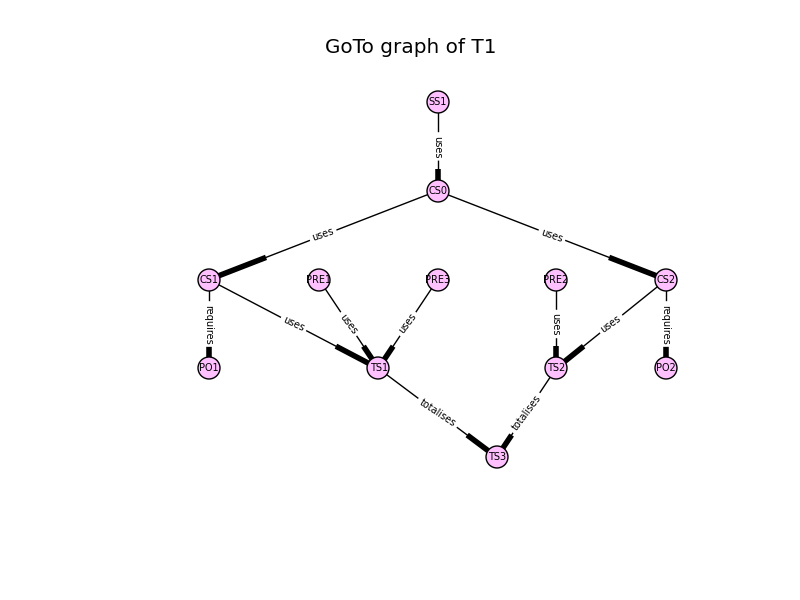
\includegraphics[scale=0.6]{Figures/zdra/gotograph.png}
\caption{An example of a goto graph \gls{zdra} correct. \label{fig:gotograph}}
\end{figure}

An example of a \emph{goto graph} is shown in figure \ref{fig:gotograph}, it is
very similar to the \emph{dependency graph}. The \emph{goto graph} also uses the
boxes created by the \gls{zdra} annotations \verb|draschema| and \verb|draline|.
However the only slight difference is the directions the edges are pointing to
in some of the relations. For example if we had the relation
\verb|\initialOf{IS1}{SS1}|, in the compiled document and in the
\emph{dependency graph} the arrow will be going from \verb|IS1| to \verb|SS1|
this is because it is indeed true that the initial schema \verb|IS1| is the
\textbf{initial of} the state schema \verb|SS1|. On the other hand, in the
\emph{goto graph} the edge is pointing the other way from the stateschema
\verb|SS1| to the initialschema \verb|IS1|. This is because the initialschema
\verb|IS1| needs \verb|SS1| to exist, that is if \verb|SS1| didn't exist then
\verb|IS1| couldn't initialize it. Therefore the instance \verb|IS1| is dependent
on \verb|SS1|.

The other \gls{zdra} relations which also reverse the direction of the arrow in
the \emph{goto graph} are \emph{uses},\emph{requires} and \emph{totalises}.

The GoTo graph represents the order the instances should go in when translating
the specification into Isabelle syntax.

The dependency and GoTo graphs contain the same instances and the same
relations, however  the direction of the relations may be different. These differences between the dependency and GoTo graphs are
described in the next chapter.

% %\section{A formal view on the \gls{zdra}.}

% % We denote the star character `*' to denote one or many. We remind the reader
% that `$\mathbf{\Gamma}$' denotes the schematext of a specification,
% $\mathcal{Z}, \mathcal{E}, \mathcal{T}$ and $\mathbb{S}$ are correctly typed
% \emph{declaration}, \emph{expression}, \emph{term} and \emph{set} respectively
% (from table \ref{tab:zcga1} in chapter \ref{ch:zcga}).

% \begin{defin}
% Let $\mathcal{E}$ be a correctly typed expression. \\ Let $\mathcal{D}$ be a
% correctly typed definition. \\
% Where $((\mathcal{Z}@\mathcal{E})$*$|\mathcal{T}$*$|\mathbb{S}$*$) \in
% \mathcal{E}$ and $(\mathcal{T}$*$|\mathbb{S}$*$) \in \mathcal{D}$\\
% Let $\mathcal{ED}$ be the set containing $\mathcal{E}$'s and $\mathcal{D}$'s.
% \end{defin}

% For example an expression can be the following: \verb|t = t| where $t$ is a
% term. Therefore this expression contains two terms. Another example of an
% expression could be: $\forall t: S \bullet t = 0$. This expression contains a
% declaration within an expression ($(\mathcal{Z}@\mathcal{E})$, which is $t:S$.


% \begin{table}[H]
% \begin{footnotesize}
% \begin{tabular}{| l | l | l |}
% \hline
% \textbf{Instance} & \textbf{Allowed weak types} & \textbf{Annotations} \\
% \hline
% \hline
% precondition & $\mathcal{ED} \in \mathbf{\Gamma}$ &
% \cgatext{\expression{\mathcal{E}}\definition{\mathcal{D}}} \\

% postcondition & $\mathcal{ED} \in \mathbf{\Gamma}$ &
% \cgatext{\expression{\mathcal{E}}\definition{\mathcal{D}}} \\

% output & $\mathcal{ED} \in \mathbf{\Gamma}$ &
% \cgatext{\expression{\mathcal{E}}\definition{\mathcal{D}}} \\

% stateInvariants & $\mathcal{ED} \in \mathbf{\Gamma}$ &
% \cgatext{\expression{\mathcal{E}}\definition{\mathcal{D}}} \\

% stateSchema & $(\mathcal{Z} \& \mathcal{ED}) | \mathcal{Z} \in \mathbf{\Gamma}$
% & $(\cgatext{\declaration{\mathcal{Z}$*$} \&
% \expression{\mathcal{E}}\definition{\mathcal{D}}}) |
% \cgatext{\declaration{\mathcal{Z}$*$}}$ \\

% theory & $(\mathcal{Z} \& \mathcal{ED}) | \mathcal{Z} \in \mathbf{\Gamma}$ &
% $(\cgatext{\declaration{\mathcal{Z}$*$} \&
% \expression{\mathcal{E}}\definition{\mathcal{D}}}) |
% \cgatext{\declaration{\mathcal{Z}$*$}}$\\

% changeSchema & $(\mathcal{Z} \& \mathcal{ED}) | \mathcal{ED} \in
% \mathbf{\Gamma}$ & $(\cgatext{\declaration{\mathcal{Z}$*$} \&
% \expression{\mathcal{E}}\definition{\mathcal{D}}}) |
% \cgatext{\expression{\mathcal{E}}\definition{\mathcal{D}}}$ \\

% totaliseSchema & $(\mathcal{Z} \& \mathcal{ED}) | \mathcal{ED} \in
% \mathbf{\Gamma}$ & $(\cgatext{\declaration{\mathcal{Z}$*$} \&
% \expression{\mathcal{E}}\definition{\mathcal{D}}}) |
% \cgatext{\expression{\mathcal{E}}\definition{\mathcal{D}}}$ \\

% axiom & $\mathcal{Z} \& \mathcal{ED} \in \mathbf{\Gamma} $ &
% $\cgatext{\declaration{\mathcal{Z}$*$} \&
% \expression{\mathcal{E}}\definition{\mathcal{D}}}$ \\

% outputSchema & $\mathcal{Z} \& \mathcal{ED} \in \mathbf{\Gamma} $ &
% $\cgatext{\declaration{\mathcal{Z}$*$} \&
% \expression{\mathcal{E}}\definition{\mathcal{D}}}$ \\

% initSchema & $\mathcal{Z} \& \mathcal{ED} \in \mathbf{\Gamma} $ &
% $\cgatext{\declaration{\mathcal{Z}$*$} \&
% \expression{\mathcal{E}}\definition{\mathcal{D}}}$ \\

% \hline
% \end{tabular}

% \end{footnotesize}
% \caption{ZCGa annotations allowed in ZDRa instances \label{tab:zcgainzdra}}
% \end{table}

% Table \ref{tab:zcgainzdra} shows which \gls{zcga} are allowed to be in certain
% \gls{zdra} instances. Where `\&' means these weak type categories must be
% included in the instance. For example a \emph{stateSchema} can be made up of one
% or more $\mathcal{Z}$ \textbf{AND} one or more $\mathcal{ED}$ \textbf{OR} one or
% more $\mathcal{Z}$ on their own. Therefore a \emph{stateSchema} can not be made
% up of $\mathcal{ED}$ on it's own.

% \paragraph{precondition, postcondition, output, stateInvariants.}
% These instances can only contain a correctly typed expression or definition
% within the schematext. There may be one or more expressions or definitions.

% \paragraph{stateSchema, theory.}
% These instances can only contain one or more correctly typed declaration
% \emph{and} one or more correctly typed expression and definition or one or more
% correctly typed declarations.

% \paragraph{changeSchema, totalise.}
% These instances can only contain one or more correctly typed declaration
% \emph{and} one or more correctly typed expression and definition or one or more
% correctly typed expressions or definitions.

% \paragraph{axiom, outputSchema, initSchema}
% These instances can only contain one or more correctly typed declarations
% \emph{and} one or more correctly typed expression and definitions.

% \subsection{Allowances when combining the ZCGa and ZDRa}

% Since we have formally outlined the \gls{zdra} in table \ref{tab:zcgainzdra} we
% can now show some rules which occur when we combing the \gls{zcga} and
% \gls{zdra} together.

% \begin{thm}
% Using table \ref{tab:zcgainzdra}, the initialOf relation only permits the
% annotations: \\
%  $\mathcal{Z} \& \mathcal{ED}, initialOf, (\mathcal{Z} \& \mathcal{ED}) |
%  \mathcal{Z}$.
% \end{thm}

% \begin{proof}
% From table \ref{tab:relationsallowed} (section \ref{subsec:zdrarelations}) we
% can see the only legal relation for initialOf is `initSchema $\longrightarrow$
% stateSchema'. An initSchema can only have the annotation $\mathcal{Z} \&
% \mathcal{ED}$ and a stateSchema can only have the annotations $(\mathcal{Z} \&
% \mathcal{ED}) | \mathcal{Z}$ (from table \ref{tab:zcgainzdra}). Since
% $\longrightarrow$ represents the relation \emph{initialOf} then we get
% $\mathcal{Z} \& \mathcal{ED}, initialOf, ((\mathcal{Z} \& \mathcal{ED}) |
% \mathcal{Z})$.
% \end{proof}

% \begin{thm}
% Using table \ref{tab:zcgainzdra}, the allows relation only permits the
% annotations: \\
% $\mathcal{ED}, allows, \mathcal{ED}$.
% \end{thm}

% \begin{proof}
% The allows relation only permits `precondition $\longrightarrow$ postcondition'
% (table \ref{tab:relationsallowed}). Both a precondition and postcondition have
% the \gls{zcga} annotations $\mathcal{ED}$. Since $\longrightarrow$ represents
% the relation. Then the result is $\mathcal{ED}, allows, \mathcal{ED}$.
% \end{proof}

% \begin{thm}
% Using table \ref{tab:zcgainzdra}, the requires relation only permits the
% annotations:
% \begin{itemize}
% \item $\mathcal{Z} \& \mathcal{ED}, requires, \mathcal{ED}$
% \item $(\mathcal{Z} \& \mathcal{ED}) | \mathcal{ED}, requires, \mathcal{ED}$
% \end{itemize}
% \end{thm}

% \begin{proof}
% Using table (table \ref{tab:relationsallowed}) of permitted relations the
% requires relation has the following syntax:
% \begin{enumerate}
% \item `outputSchema $\longrightarrow$ precondition'
% \item `outputSchema $\longrightarrow$ output', 
% \item `changeSchema $\longrightarrow$ precondition', 
% \item `changeSchema $\longrightarrow$ postcondition', 
% \end{enumerate} 
% \begin{itemize}

% \item Using the allowed \gls{zcga} annotations in table \ref{tab:zcgainzdra} we
% can see that an outputSchema contains only $\mathcal{Z} \& \mathcal{ED}$ and a
% precondition and output both only contain $\mathcal{ED}$ thus 1 and 2 become
% $\mathcal{Z} \& \mathcal{ED} \longrightarrow \mathcal{ED}$. Since
% $\longrightarrow$ represents the relation then we end up with $\mathcal{Z} \&
% \mathcal{ED}, requires, \mathcal{ED}$.

% \item The allowed \gls{zcga} annotations for changeSchema are $(\mathcal{Z} \&
% \mathcal{ED}) | \mathcal{ED}$ and the allowed \gls{zcga} annotations for both
% precondition and postcondition are $\mathcal{ED}$ therefore we end up with
% ($(\mathcal{Z} \& \mathcal{ED}) | \mathcal{ED} \longrightarrow \mathcal{ED}$.
% Again the $\longrightarrow$ represents the relation so the $\longrightarrow$
% becomes `requires' and we are left with $(\mathcal{Z} \& \mathcal{ED}) |
% \mathcal{ED}, requires, \mathcal{ED}$.
% \end{itemize}
% \end{proof}

% \begin{thm}
% Using table \ref{tab:zcgainzdra}, the totalises relation only permits the
% annotations:
% \begin{itemize}
% \item $(\mathcal{Z} \& \mathcal{ED}) | \mathcal{ED}), totalises, (\mathcal{Z} \&
% \mathcal{ED}) | \mathcal{ED}$
% \item $(\mathcal{Z} \& \mathcal{ED}) | \mathcal{ED}), totalises, \mathcal{Z} \&
% \mathcal{ED}$
% \end{itemize}
% \end{thm}

% \begin{proof}
% Using table (table \ref{tab:relationsallowed}) of permitted relations the
% totalises relation has the following syntax:
% \begin{enumerate}
% \item `totaliseSchema $\longrightarrow$ changeSchema'
% \item `totaliseSchema $\longrightarrow$ outputSchema'
% \item `totaliseSchema $\longrightarrow$ totaliseSchema'
% \end{enumerate} 

% \begin{itemize}
% \item Table \ref{tab:relationsallowed} shows the \gls{zcga} syntax for
% totaliseSchema and changeSchema is $(\mathcal{Z} \& \mathcal{ED}) |
% \mathcal{ED})$. Thus the permitted relations would be $(\mathcal{Z} \&
% \mathcal{ED}) | \mathcal{ED}) \longrightarrow (\mathcal{Z} \& \mathcal{ED}) |
% \mathcal{ED})$ for points 1 and 3. Since $\longrightarrow$ represents the
% relation `totalises' in this case we would have $(\mathcal{Z} \& \mathcal{ED}) |
% \mathcal{ED}), totalises, (\mathcal{Z} \& \mathcal{ED}) | \mathcal{ED})$. Hence
% the first part of the theorem is proven.

% \item Output schema has the \gls{zcga} syntax $(\mathcal{Z} \& \mathcal{ED})$
% according to table \ref{tab:zcgainzdra}. If totaliseSchema has the \gls{zcga}
% syntax $(\mathcal{Z} \& \mathcal{ED}) | \mathcal{ED})$ then using point 2 the
% permitted relation would be $(\mathcal{Z} \& \mathcal{ED}) | \mathcal{ED})
% \longrightarrow \mathcal{Z} \& \mathcal{ED}$. Again since $\longrightarrow$
% represent totalise in this case we conclude with $(\mathcal{Z} \& \mathcal{ED})
% | \mathcal{ED}), totalises, \mathcal{Z} \& \mathcal{ED}$.
% \end{itemize}
% \end{proof}

% \begin{thm}
% Using table \ref{tab:zcgainzdra}, the uses relation only permits the
% annotations:
% \begin{itemize}
% \item $\mathcal{Z} \& \mathcal{ED}, uses, (\mathcal{Z} \& \mathcal{ED}) |
% \mathcal{Z}$
% \item $(\mathcal{Z} \& \mathcal{ED}) | \mathcal{ED}, uses, (\mathcal{Z} \&
% \mathcal{ED}) | \mathcal{Z}$
% \item $(\mathcal{Z} \& \mathcal{ED}) | \mathcal{Z}, uses, (\mathcal{Z} \&
% \mathcal{ED}) | \mathcal{Z}$
% \item $(\mathcal{Z} \& \mathcal{ED}) | \mathcal{Z}, uses, \mathcal{Z} \&
% \mathcal{ED}$
% \item $\mathcal{Z} \& \mathcal{ED}, uses, \mathcal{Z} \& \mathcal{ED}$
% \item $(\mathcal{Z} \& \mathcal{ED}) | \mathcal{ED}, uses, \mathcal{Z} \&
% \mathcal{ED}$
% \end{itemize}
% \end{thm}

% \begin{proof}
% Using table (table \ref{tab:relationsallowed}) of permitted relations the uses
% relation has the following syntax:
% \begin{enumerate}
% \item `outputSchema $\longrightarrow$ stateSchema'
% \item `changeSchema $\longrightarrow$ stateSchema'
% \item `stateSchema $\longrightarrow$ stateSchema'
% \item `stateSchema $\longrightarrow$ axiom'
% \item `outputSchema $\longrightarrow$ axiom'
% \item `changeSchema $\longrightarrow$ axiom'
% \end{enumerate} 

% \begin{itemize}
% \item According to table \ref{tab:zcgainzdra} the \gls{zcga} syntax for
% outputSchema is $\mathcal{Z}\&\mathcal{ED}$ and the syntax for stateSchema is
% $(\mathcal{Z} \& \mathcal{ED}) | \mathcal{Z}$. Therefore using point 1 we get
% `$\mathcal{Z}\&\mathcal{ED} \longrightarrow (\mathcal{Z} \& \mathcal{ED}) |
% \mathcal{Z}$'. Since $\longrightarrow$ represents the relation uses in this case
% we get $\mathcal{Z} \& \mathcal{ED}, uses, (\mathcal{Z} \& \mathcal{ED}) |
% \mathcal{Z}$.

% \item The syntax for changeSchema is $(\mathcal{Z} \& \mathcal{ED}) |
% \mathcal{ED}$ and the syntax for stateSchema is $(\mathcal{Z} \& \mathcal{ED}) |
% \mathcal{Z}$ according from table \ref{tab:zcgainzdra}. Substituting the
% \gls{zcga} for instance names in point 2 we get $(\mathcal{Z} \& \mathcal{ED}) |
% \mathcal{ED} \longrightarrow (\mathcal{Z} \& \mathcal{ED}) | \mathcal{Z}$. By
% substituting the relation uses for $\longrightarrow$ we end up with
% $(\mathcal{Z} \& \mathcal{ED}) | \mathcal{ED}, uses, (\mathcal{Z} \&
% \mathcal{ED}) | \mathcal{Z}$.

% \item Using table \ref{tab:zcgainzdra} the \gls{zcga} syntax for stateSchema is
% $(\mathcal{Z} \& \mathcal{ED}) | \mathcal{Z}$. Using point 3, we substitute the
% \gls{zcga} syntax for the instance name and we get $(\mathcal{Z} \&
% \mathcal{ED}) | \mathcal{Z} \longrightarrow (\mathcal{Z} \& \mathcal{ED}) |
% \mathcal{Z}$. Since $\longrightarrow$ represents uses then we get $(\mathcal{Z}
% \& \mathcal{ED}) | \mathcal{Z}, uses, (\mathcal{Z} \& \mathcal{ED}) |
% \mathcal{Z}$.

% \item The \gls{zcga} syntax for stateSchema is $(\mathcal{Z} \& \mathcal{ED}) |
% \mathcal{Z}$ and the \gls{zcga} syntax for axiom is  $\mathcal{Z} \&
% \mathcal{ED}$. By substituting these \gls{zcga} syntax's in point 4 we get
% $(\mathcal{Z} \& \mathcal{ED}) | \mathcal{Z} \longrightarrow \mathcal{Z} \&
% \mathcal{ED}$. Since $\longrightarrow$ in this case is the relationship uses, we
% can change $\longrightarrow$ to `uses' and get $(\mathcal{Z} \& \mathcal{ED}) |
% \mathcal{Z}, uses, \mathcal{Z} \& \mathcal{ED}$.

% \item According to table \ref{tab:zcgainzdra} the \gls{zcga} syntax for
% outputSchema and axiom are both $\mathcal{Z} \& \mathcal{ED}$. Therefore if we
% put in the \gls{zcga} syntax instead of the instance names in point 5 we get
% $\mathcal{Z} \& \mathcal{ED} \longrightarrow \mathcal{Z} \& \mathcal{ED}$. From
% table \ref{tab:relationsallowed} we can deduce that $\longrightarrow$ mean
% `uses' so we finish with $\mathcal{Z} \& \mathcal{ED}, uses, \mathcal{Z} \&
% \mathcal{ED}$.

% \item Finally, the \gls{zcga} syntax for changeSchema is $(\mathcal{Z} \&
% \mathcal{ED}) | \mathcal{ED}$ and the \gls{zcga} syntax for axiom is
% $\mathcal{Z} \& \mathcal{ED}$ according to table \ref{tab:zcgainzdra}. If we
% substitute the allowed \gls{zcga} syntax in point 6 we get $(\mathcal{Z} \&
% \mathcal{ED}) | \mathcal{ED} \longrightarrow \mathcal{Z} \& \mathcal{ED}$. Since
% $\longrightarrow$ is the relation `uses' in this case we end up with
% $(\mathcal{Z} \& \mathcal{ED}) | \mathcal{ED}, uses, \mathcal{Z} \&
% \mathcal{ED}$.
% \end{itemize}
% \end{proof}

\section{Conclusion}
In this chapter the \gls{zdra} step of the \gls{zmath} has been described. A
\LaTeX{} style package has been created to allow a user to annotate a Z
specification and see the structure of the system. A \gls{zdra} program has been
created to check for rhetorical correctness and make sure there are no loops in
the reasoning of the specification. Warning messages appear if the specification
is still lacking some totalising schemas for some preconditions. We have also
formally outlined the \gls{zdra} and shown some rules which occur when combining
the \gls{zcga} and \gls{zdra} together. If the specification is correct at the
\gls{zdra} stage then the user may then go on to create general and theorem
prover specific skeletons which are described in the next chapter.
%\chapter{From ZDRa to General Proof Sketch}
\label{ch:skeletons}

The skeletons described in this chapter are automatically generated if the specification passes the \gls{zdra} check. Section \ref{sec:zdra2gen} describes the general proof skeleton. Which uses the graphs generated in the \gls{zdra} to provide the order the instaces should go to into any theorem prover. Section \ref{chap:gpsa2isa} then explains how a general proof skeleton can be automatically translated into a skeleton in Isabelle format automatically. In section \ref{sec:isa2ful} we describe how the Isabelle Skeleton can be used to fully prove a formal specification which requires two steps, the first is an automatic step to fill in the Isabelle skeleton and the final step is up to the user to prove the lemma's and properties of the specification.

\section{What is a General Proof Sketch}
\label{sec:zdra2gen}

When checking for ZDRa correctness the program adds all the annotated chunks into a dependency graph and a GoTo graph. Both these graphs are directed graphs.

We then run an algorithm on the GoTo graph to generate a proof skeleton. Figure \ref{fig:code} shows part of the code in generating this proof sketch.

\begin{itemize}
\item \textit{allnodes}, is a set of all the instances labelled by the user of a specification in ZDRa.

\item \textit{fromnodes}, is a set containing all the nodes which are dependent on another instance.

\item \textit{tonodes}, is a set containing all the nodes which have some other nodes dependent on them.
\end{itemize}

\begin{figure}[H]
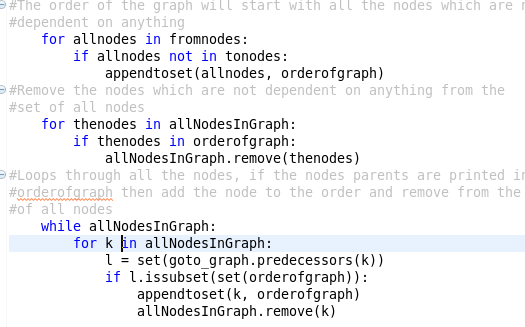
\includegraphics[scale=0.5]{Figures/skeleton/code.png}
\caption{Part of the algorithm to create a proof sketch.}
\label{fig:code}
\end{figure}

\section{Creating the Graph}

Here we show how a Proof skeleton is calculated using the Goto graph created when running the ZDRa check on a specification.

\begin{figure}[H]
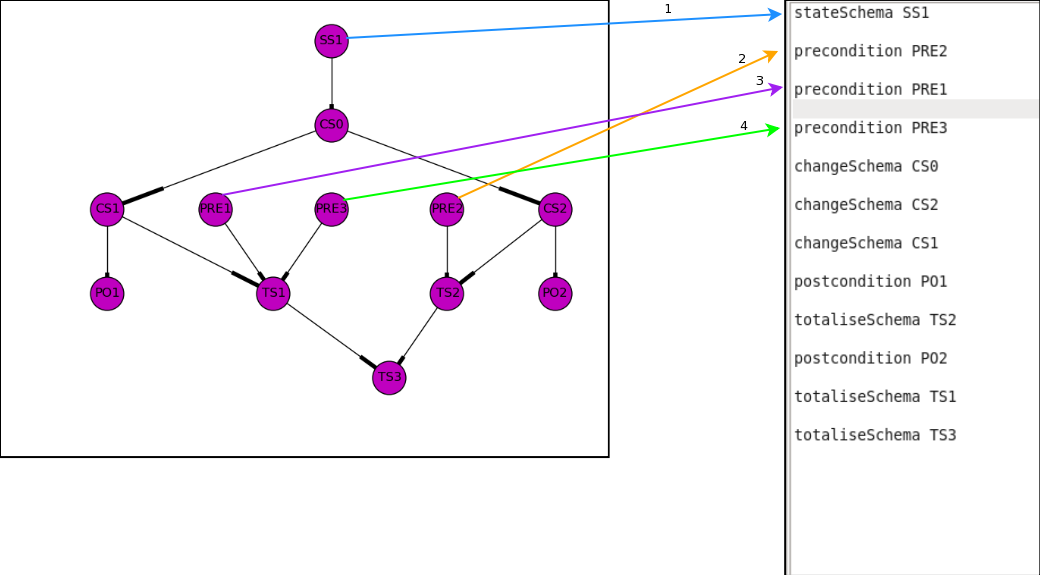
\includegraphics[scale=0.3]{Figures/skeleton/1.png}
\caption{GoTo graph and proof skeleton of vending machine step 1.}
\label{fig:1}
\end{figure}

First of all the program looks at all the nodes of the GoTo graph and prints out all the nodes which are not dependent on anything. That is, they may have successors but they have no predecessors, they do not use or need anything else and can stand by themselves. These nodes can be printed in any order, so in diagram \ref{fig:1} we see that we have SS1, PRE1 PRE2 and PRE3 all printed.

\begin{figure}[H]
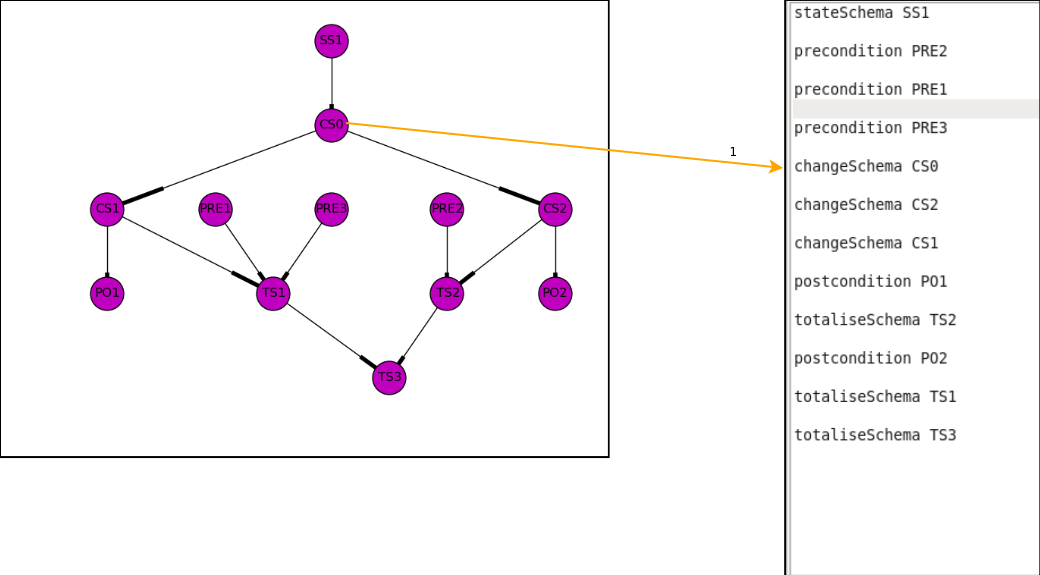
\includegraphics[scale=0.3]{Figures/skeleton/2.png}
\caption{GoTo graph and proof skeleton of vending machine step 2.}
\label{fig:2}
\end{figure}

The next part of the algorithm checks whether there exists a node in the GoTo graph where all of its parents are printed out in the proof skeleton. Figure \ref{fig:2} shows that the next node to be in the proof skeleton is CS0. 

\begin{figure}[H]
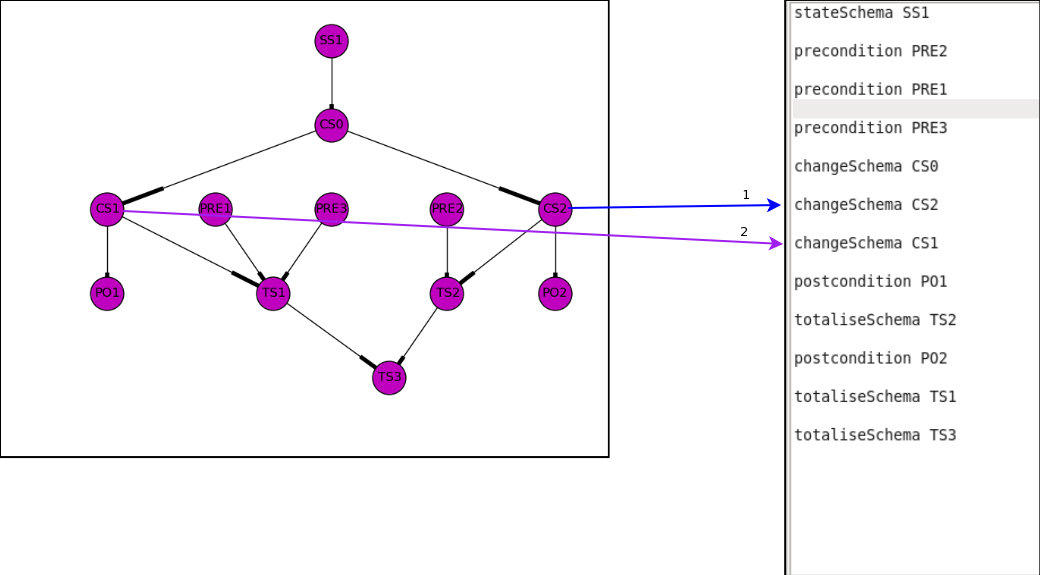
\includegraphics[scale=0.3]{Figures/skeleton/3.png}
\caption{GoTo graph and proof skeleton of vending machine step 3.}
\label{fig:3}
\end{figure}

The next part we see that after CS0 is added to the proof skeleton then both CS1, and CS2 can be added. This is shown in figure \ref{fig:3}.

\begin{figure}[H]
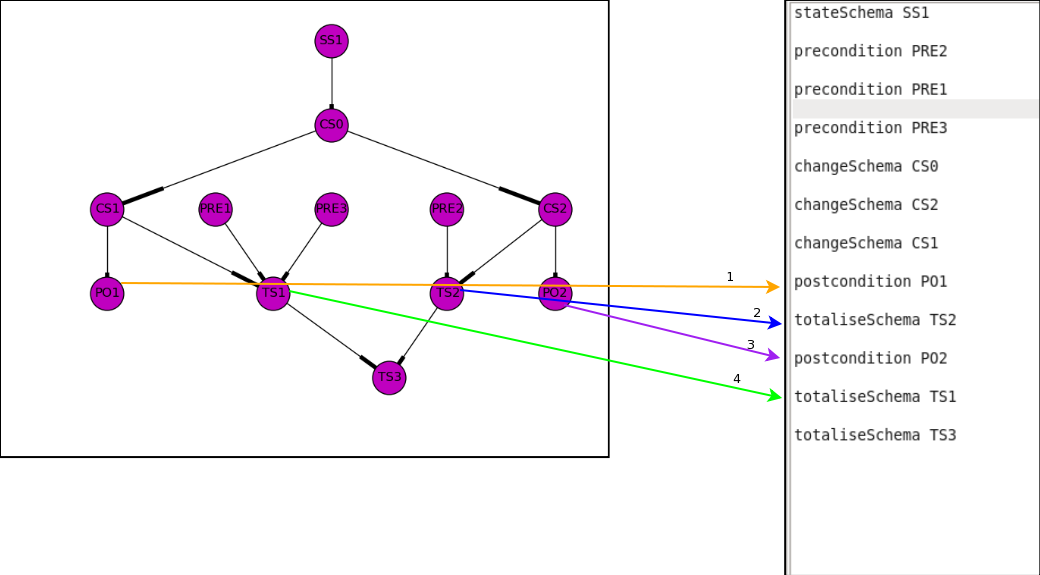
\includegraphics[scale=0.3]{Figures/skeleton/4.png}
\caption{GoTo graph and proof skeleton of vending machine step 4.}
\label{fig:4}
\end{figure}

Figure \ref{fig:4} shows the next stage of adding nodes to the Proof Skeleton. Since CS1 and CS2 are now added to the proof skeleton then the next row of nodes can be added. Since PO1 only had one parent (CS1) it is added first, PO2 also had one parent (CS2) it is added second. The others had more parents which are already in the proof sketch so they are added next randomly.

\begin{figure}[H]
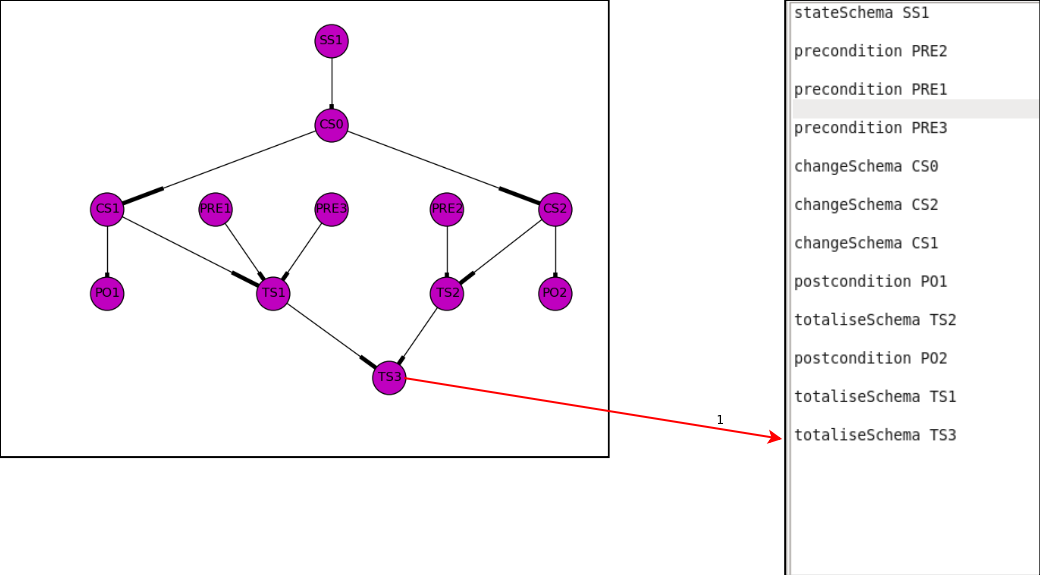
\includegraphics[scale=0.3]{Figures/skeleton/5.png}
\caption{GoTo graph and proof skeleton of vending machine step 5.}
\label{fig:5}
\end{figure}

We come to the final stage of the dependency graph, when all the nodes are in the dependency graph except for one which is added to the end.

\section{Proof Obligations}

There are many properties one may wish to prove about their specification. These certain properties are called proof obligations. Proof obligations for formal notations are an entire research area in their own right. However as the \gls{zmath} framework concentrates on giving the novice an idea of how to prove their specification we will focus on checking the specification for consistancy. Using the description in \cite{DBLP:conf/icsea/WenMZ06}, checking the specification is consitant can fall under two categories:

\begin{itemize}
\item POb1, Feasability of an operation
\item POb2, Other specific proof obligation for the chosen specification
\end{itemize}

We use the syntax \textit{Context} $\vdash$ \textit{predicate} taken from the paper to define the proof obligations.

\subsection{POb1, Proof Obligation type 1}

\begin{defin}\label{defa}POb1\\

$Context \vdash \exists var, var' \bullet PRE\# \land PO\# \longrightarrow SI\# \land SI\#'$\\

\noindent where var and var' are the variables and variables' used in the schema with their types, SI\# is the state Invariants of the specification, SI\#' is the state invariants prime in the specification, PRE\# is the precondition of the schema, PO\# is the post operation of the schema and \# is some arbitary number.
\end{defin}

POb1 shows the feasability of an operation. When an operation can transfor a state to another state in the state space (a $\Delta$ schema). If an operation is feasible, the preconditional state and postconditional state should satisfy the state invariants of the specification.

Again by using the ModuleReg specification we can see a proof obligation is needed when adding a student doesnt change the state invariants of the specification.

\begin{verbatim}
lemma AddStudentDoesntChangeSI:
"(\<exists> taking taking'  :: (PERSON * MODULE) set.
 \<exists> degModules degModules':: MODULE set.
 \<exists> students students':: PERSON set.
  \<exists> p :: PERSON.
(students' = students \<union> {(p)}) 
\<and> (taking' = taking)
\<and> (degModules' = degModules)
\<longrightarrow> ((Domain taking \<subseteq> students)
\<and> (Range taking \<subseteq> degModules)
\<and> (Domain taking' \<subseteq> students')
\<and> (Range taking' \<subseteq> degModules'))) "
\end{verbatim}

The ZDRa syntax of this proof obligation would be :

\begin{verbatim}
lemma AddStudentDoesntChangeSI:
" \<exists> (*CS1_variables :: CS1_TYPES*).
(PRE1)
\<and> (PO1)
\<longrightarrow> ((SI1)
\<and (SI1'))"
\end{verbatim}

 The ZDRa syntax of the proof obligation stays that there exists some variables of the operational schema where the precondition (PRE1) \emph{and} postCondition (PO1) imply that the stateInvariants (SI1) and stateInvariants prime hold.

\subsection{POb2, Proof Obligation type 2}

As POb2 are any other relevent properties users wish to prove about the specification we can not formally define it. However an example would be if there existed a specification where an operator which added a member to a club and then removed a member from the club. Then the amount of members should be the same after both operators have completed the task.

One such example is in the ModuleReg specification the RegForModule schema postcondition shows that \verb|(taking' = taking ∪ {(p, m)}) | therefore if this were to happen then we should make sure that \verb|taking'| is not empty after the operation. This proof obligation is very specific to the ModuleReg specification and the user would need to write and check this themselves. To do such we have the following lemma:

\begin{verbatim}
lemma notEmpty:
"(taking' = taking \<union> {(p,m)}) 
\<longrightarrow> (taking' \<noteq> {})"
\end{verbatim}

Where the name of the lemma is \verb|notEmpty| then the postOperation of the ChangeSchema is \verb|(taking' = taking \<union> {(p,m)}) | then checking that the set is not empty follows the right arrow \verb|(taking' \<noteq> {})|.

POb1 can be automate. Since POb2 is specification specific, each user will need to define these themselves if they so wish.

\subsection{Proof Obligations in the General Proof Skeleton}

Since the POb2 are specific to the specification only POb1 are automatically added. They are generated as `\emph{lemma's}' in the general proof skeleton. 

\begin{figure}[H]
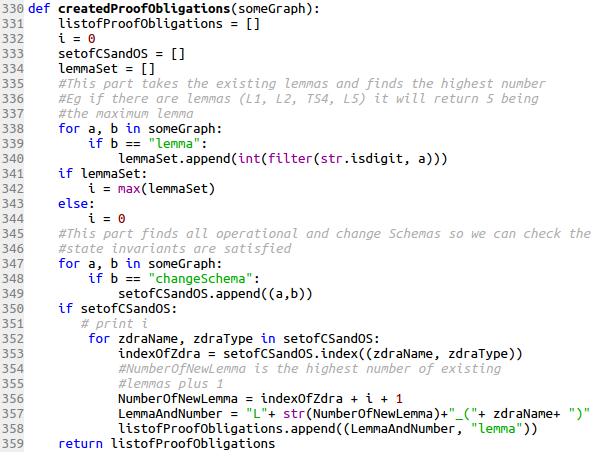
\includegraphics[scale=0.6]{Figures/skeleton/pobcode.png}
\caption{Part of the algorithm to create Proof Obligation ZDRa names.}
\label{fig:codepob}
\end{figure}

The proof obligations which check that changeSchema's and outputSchema's follow the stateInvariants are added to the original general proof skeleton. The general proof skeleton starts of with being an ordered list (GPSaOL), then the algorithm for generating a list of proof obligations is run and added to the original proof skeleton. Figure \ref{fig:codepob} shows the algorithm which creates the ordered list of proof obligations.

Lines 338-344 find all the existing lemma's in the \gls{gpsol} and sets \emph{i} to be the highest number. For example if there are existing lemmas in \gls{gpsol} (L1, L2, L3), then \emph{i} becomes 3. If there are no existing lemmas in \gls{gpsol} then \emph{i} stays as 0. Lines 347-250 take all the elements which are \emph{changeSchema} instances and adds them to a list of \emph{setCSandOS}. Then lines 350-359 loops through all the changeSchema's, takes the \gls{zdra} name, add's L + a number + \gls{zdra} name and adds it to the \emph{listOfProofObligations}.

\paragraph{For Example}

if we had the following \gls{gpsol}: \\
\noindent [(SS1, stateSchema), (IS1, initialSchema), (CS1, changeSchema), (CS2, changeSchema), (TS1, totaliseSchema)] \\
Then in this case:
\begin{itemize}
\item lemmaSet = []
\item i = 0
\item setofCsandOs = [(CS1, changeSchema), (CS2, changeSchema)]
\end{itemize}

Then for each element in setofCsandOs we would add the new elements (L1\_CS1, lemma) and (L2\_CS2, lemma) to the ordered list \emph{listOfProofObligations}.

The new \gls{gpsol} would then become [(SS1, stateSchema), (IS1, initialSchema), (CS1, changeSchema), (CS2, changeSchema), (TS1, totaliseSchema), (L1\_CS1, lemma) and (L2\_CS2, lemma)]

If for example the original \gls{gpsol} was \\
\noindent [(SS1, stateSchema), (IS1, initialSchema), (CS1, changeSchema), (CS2, changeSchema), (TS1, totaliseSchema), (L1, lemma), (L2, lemma)]\\
Then then new proof obligation lemmas would be (L3\_CS1, lemma) and (L4\_CS2, lemma) as we would already have L1 and L2.

\begin{figure}[H]
\centering
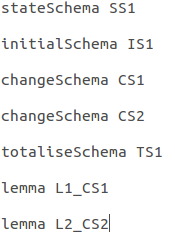
\includegraphics[scale=0.5]{Figures/skeleton/proofskeletonwithpo.png}
\caption{Example of a General Proof Skeleton with lemma's.}
\label{fig:gpswithpo}
\end{figure}

An example of a General Proof Skeleton with added proof obligations is shown in Figure \ref{fig:gpswithpo}. The changeSchema's in this specification are CS1 and CS2. Therefore to make sure the changeSchemas do not change the state of the specification and comply with the state invariants the two lemma's L1\_CS1 and L2\_CS2 have been added.

\subsubsection{Proof Obligations in specification examples}
Since the vending machine specification (appendix \ref{app:vm2}) doesn't have any stateInvaritants then the \gls{gps} will not have any added proof obligations to check for consistance. That is we can't check that the postconditions do not change the state if the state has no restrictions. However the birthdaybook example (appendix \ref{app:bb3}) does have stateInvariants. Therfore we must add properties to check that any changeSchema's follow the state restrictions. Part of the birthdaybook \gls{gps} is shown in figure \ref{fig:bbgps}. Since there are stateInvariants (SI1) and a changing state Schema (CS1) then the proof obligation \texttt{L1\_(CS1)} has been added to the \gls{gps}.

\begin{figure}[H]
\begin{verbatim}
stateSchema SS1 
stateInvarients SI1 
initialSchema IS1 
postcondition PO2 
outputSchema OS1 
precondition PRE2 
changeSchema CS1 
totaliseSchema TS1 
.......
lemma L1_(CS1) 
\end{verbatim}
\caption{Part of the GPSa for the birthdayBook example. (Full version shown in appendix \ref{app:bb3}) \label{fig:bbgps}}
\end{figure}

\section{Conclusion}
\label{sec:skeletonsConclusion}

This chapter describes how the \gls{zdra} program uses the GoTo graph to generate a general proof skeleton (step 2$\rightarrow$3 in figure \ref{fig:steps}). The general proof skeleton is an automatically generated .txt file which displays the order in which this instances must go in a theorem prover to be logically correct. This chapter gives a basic understanding of proof obligations for Z and examples which proof obligations are automatically generated when translating Z specifications into Isabelle. We give a formal definition of the proof obligation to check for consistancy of the state invariants and show an example. The next chapter describes how the general proof skeleton is translated into Isabelle syntax.
%\chapter{General Proof Sketch aspect and beyond}
\label{chap:gpsa2isa}

 In this section we outline how the Z specification is
translated into Isabelle. If the user has labelled a theory in the specification (T\#) then that will
begin writing an Isabelle skeleton.
For example if we had an empty specification (without a context) and named it `\texttt{a}' then the program
will create an empty Isabelle skeleton e.g.

\begin{verbatim}
theory gpsa_a
imports
main
begin
end
\end{verbatim}

If the user labels a schema `\texttt{SS1}' meaning the stateSchema of the
specification then that in Isabelle becomes a `\texttt{record}' and a
`\texttt{locale}' is created. Using our example of specification named
`\texttt{a}' we get the following (after the premuable described before):
\begin{verbatim}
record SS1 =
(*DECLARATIONS*)
locale a =
fixes (*GLOBAL DECLARATIONS*)
assumes SI#
begin
end
end
\end{verbatim}

If there are no state invariants in the state schema at this point then there is
no `\texttt{assumes SI\#}') line.

All other schemas including changeSchemas, outputSchemas, preconditions that are
schemas, post conditions that are schemas and all other state schema become
definitions in the Isabelle skeleton. So for example if we have the following
schema written in \gls{zdra}:
\begin{verbatim}
\draschema{CS1}{
\begin{schema}{b}
someDeclaration
\where
\draline{PO1}{someExpression}
\end{schema}}
\end{verbatim}

Then when translating into the Isabelle skeleton it becomes:
\begin{verbatim}
definition CS1 ::
"(*CS1_TYPES*) => bool"
where
"CS1 (*CS1_VARIABLES*) == PO1"
\end{verbatim}

At this stage it doesn't matter what the declarations and expressions are as
they get filled in at the next stage. The Isabelle skeleton only uses the
\gls{zdra} labels to be created.

Totalising schemas, written either horizontally or vertically in a specification
become definitions when translating into the Isabelle skeleton. For example if
we have the following totalisingSchema:

\verb|\draline{TS1}{someSchema == someExpression}|

This would translate to the Isabelle skeleton as:

\begin{verbatim}
definition TS1 ::
"(*TS1_TYPES*) => bool"
where
"TS1 (*TS1_VARIABLES*) == (*TS1_EXPRESSION*)"
\end{verbatim}

Again, at this stage it doesn't matter what the expression is. As it gets filled
in at the next stage.

\section{Proof Obligations in Isabelle Syntax}

Lemmas which are proof obligations- that is instances with the a \gls{zdra} name
\texttt{L\#\_CS\#} where `\texttt{\#}' is a number become \texttt{lemma's} in
Isabelle syntax. The translation from the \gls{gpsa} into Isabelle syntax
depends if the changeSchema in question has a precondition, postcondition or
both. We use definition \ref{defa} in aid with the translation.

\subsection{Proof Obligation translation where the schema has a precondition}

If the changeSchema in which the proof obligation is about has a precondition as
well as a postcondition then the translation will be as follows. 

If an instance has the \gls{zdra} name `\texttt{L1\_CS1}' and we have the
relations (CS1, requires, PRE1), (PRE1, allows, PO2) and (CS1, uses, IS1) then
the Isabelle skeleton syntax would be as follows:

\begin{verbatim}
lemma L1_CS1:
" \<exists> (*CS1_variables :: CS1_TYPES*).
(PRE1)
\<and> (PO2)
\<longrightarrow> ((SI1)
\<and (SI1'))"
sorry
\end{verbatim}

We use the Isabelle word `\texttt{sorry}' to tell the theorem prover to skip a
proof-in-progress and to treat the goal under consideration to be proved. This
then causes the Isabelle skeleton to be an incorrect document but is a goal the
user may prove at a later stage after the skeleton has been filled in.

If the instance in the \gls{gpsa} was `\texttt{L1\_CS1}' and the relationship
only had a precondition and no post condition ie (CS1, requires, PRE1) and (CS1,
uses, IS1) but not the allows relationship the syntax in the Isabelle skeleton
would be 

\begin{verbatim}
lemma L1_CS1:
" \<exists> (*CS1_variables :: CS1_TYPES*).
(PRE1)
\<longrightarrow> ((SI1)
\<and (SI1'))"
sorry
\end{verbatim}

Where SI1 is the stateInvariants used in the stateSchema and SI1' is the
stateInvariants prime.

\subsection{Proof Obligation translation where the changeSchema has only postcondition}

If the instance in the \gls{gpsa} was L1\_CS1 and CS1 only required a
postcondition with no precondition i.e. had the relation (CS1, requires, PO2)
and (CS1, uses, IS1) then the syntax in the Isabelle skeleton would be as
follows:

\begin{verbatim}
lemma L1_CS1:
" \<exists> (*CS1_variables :: CS1_TYPES*).
(PO2)
\<longrightarrow> ((SI1)
\<and (SI1'))"
sorry
\end{verbatim}

Where PO2 is the postcondition the changeSchema requires, SI1 is the
stateInvariants in the stateSchema and SI1' is the stateInvariants prime. 

%\section{Benefits}

%The Isabelle skeleton allows for incomplete specifications to also be automated
%into a half-baked proof. This way the user can have a general outline for their
%specification and fill in the missing information directly into the Isabelle
%skeleton at a later stage. For this reason it is good to have an Isabelle
%skeleton before the full filled in half-baked proof. The user then has an
%outline if they wish to add to the specification directly as they will have an
%example of how the instances should be translated. An example of a semi formal
%specification which has been translated to step 5 (the half baked proof) is
%shown in appendix \ref{app:semiform}. Although this specification is not fully
%formal its grammatical correctness and rhetorical correctness can be checked. It
%can also start being translated into Isabelle syntax. The dependencies are shown
%between the current instances and the user can see what other information needs
%to be added for the specification to be complete.

\section{ZCGa specification to Fill in the Isabelle Skeleton}
\label{sec:zcga2fillin}

Since translating using ZMathLang can even been done on incomplete specifications, it is important to
note that if some information is missing e.g. a declaration, expression
etc then the comments of where these should go will not be changed. For example
if we have the line \verb|"(*CS1_TYPES*) => bool"| in the skeleton and the
schema CS1 has no declarations yet then the line will not be changed, and it is
up to the user to input the variables and the types of that definition.

It is important to note that all the \gls{zcga} annotations at this stage
disappear as the labelled information is automatically put into Isabelle syntax.

\subsection{Types and Freetypes in Z}

The program which fills in the Isabelle skeleton goes through the entire
specification and adds any Z declared types and freetypes before the record. For
example, if a specification has the following:
\begin{verbatim}
\begin{zed}
[STUDENT]
\end{zed}
\end{verbatim}

Then the line \verb|typedecl STUDENT| will be added after the first begin in the
skeleton.

If the specification had the following freetype:
\begin{verbatim}
\begin{zed} 
REPORT ::= ok | already\_known | not\_known
\end{zed}
\end{verbatim}

Then again, in the same place as the Z-Types the line
\begin{verbatim}
datatype  REPORT = ok | already_known | not_known
\end{verbatim}
is added to the skeleton.

\subsection{Declarations}

In Isabelle the types and variables are added separately. For instance if we had
the following schema:

\begin{verbatim}
\draschema{OS1}{
\begin{schema}{ab}
d: \power COLOUR
c: COLOUR
\where
\draline{PO1}{c \in d}
\end{schema}}
\end{verbatim}

Then the Isabelle skeleton for this schema will be as follows:

\begin{verbatim}
definition OS1 ::
"(*OS1_TYPES*) => bool"
where
"OS1 (*OS1_VARIABLES*) == (PO1)"
\end{verbatim}

Since we have two declarations, the filling in program would change the
definition in the skeleton as follows:

\begin{verbatim}
definition ab ::
"COLOUR set => COLOUR => bool"
where
"ab d c == (c \<in> d)"
\end{verbatim}

Therefore, from the declarations, the types replace the line
\verb|(*OS1_TYPES*)| and the variables replace the line
\verb|(*OS1_VARIABLES*)|.

\subsection{Expressions}

Since the majority of the syntax for expressions is very similar to the syntax
in Isabelle, the expressions are put in directly with minor changes. The
expressions replace the \gls{zdra} labellings.

Using our previous example shown in the last section, we have the schema
`\texttt{ab}', in the skeleton we have a label `\texttt{PO1}' which is then
replaced by the expression \verb|c \<in> d|. Note this expression is very
similar to the expression in \LaTeX{} \verb|c \in d| apart from the symbol
\verb|\in| becomes \verb|\<in>|. Table \ref{tab:latextoisabelle} shows the rest
of these automatic changes of the syntax made from \LaTeX{} to Isabelle.

Note: The following table shows one example of mapping Z specifications into the
Isabelle theorem prover. There may be other ways to map the syntax from \LaTeX{}
into Isabelle but we use the following table to show the proof of concept.

{\def\arraystretch{0.5}\tabcolsep=0.5pt
\begin{longtable}[H]{|c | c | c |}
\hline
\textbf{Syntax in Z} & \textbf{Syntax in \LaTeX} & \textbf{Syntax in Isabelle}
\\
\hline
\hline
$\{...\}$ & \verb|\{...\}| & \verb|{...}|\\
\hline
$\limg...\rimg$ & \verb|\limg...\rimg| & \verb|``| \\
\hline
$\langle...\rangle$ & \verb|\langle...\rangle| & \verb|\<langle>...\<rangle>| \\
\hline
$\# $ A & \verb|\#| & \verb|card| \textit{if A is set}, \\
& & \verb|length| \textit{if A is list} \\
\hline
$\cup $ & \verb|\cup| & \verb|\<union>| \\
\hline
$\cap$ & \verb|\cap| & \verb|\<inter>| \\
\hline
$\cross$ & \verb|\cross| & \verb|\<times>| \\
\hline
$\setminus$ & \verb|\setminus| & \verb|-| \\
\hline
$\geq$ & \verb|\geq| & \verb|\<ge>| \\
\hline
$\leq$ & \verb|\leq| & \verb|\<le>| \\
\hline
$\lhd$ & \verb|\lhd| & \verb|\<lhd>| \\
\hline
$\rhd$ & \verb|\rhd| & \verb|\<rhd>| \\
\hline
$\nrres$ & \verb|\nrres| & \verb|\<unlhd>| \\
\hline
$\ndres$ & \verb|\ndres| & \verb|\<unrhd>| \\
\hline
$\implies$ & \verb|\implies| & \verb|\<Longrightarrow>| \\
\hline
$\iff$ & \verb|\iff| & \verb|\<Longleftrightarrow>| \\
\hline
$\notin$ & \verb|\notin| & \verb|\<notin>| \\
\hline
$\in$ & \verb|\in| & \verb|\<in>| \\
\hline
$\subset$ & \verb|\subset| & \verb|\<subset>| \\
\hline
$\subseteq$ & \verb|\subseteq| & \verb|\<subseteq>| \\
\hline
$\land$ & \verb|\land| & \verb|\<and>| \\
\hline
$\lor$ & \verb|\lor| & \verb|\<or>| \\
\hline
$\lnot$ & \verb|\lnot| & \verb|\<not>| \\
\hline
$\neq$ & \verb|\neq| & \verb|\<noteq>| \\
\hline
$a \mapsto b$ & \verb|a \mapsto b| & \verb|(a,b)| \\
& & \verb|` '| \textit{if set preceding using} \verb|\<rightharpoonup>| \\
\hline
$\power A$ & \verb|\power A| & \verb|A set| \\
\hline
$\nat$ & \verb|\nat| & \verb|nat| \\
\hline
$\nat_1$ & \verb|\nat_1| & \verb|nat| \\
\hline
$\num$ & \verb|\num| & \verb|num| \\
\hline
$A \pfun B$ & \verb|A \pfun B| & \verb|(A \<rightharpoonup> B)| \\
\hline
$A \fun B$ & \verb|A \fun B| & \verb|(A * B) set| \\
\hline
$A \rel B$ & \verb|A \rel B| & \verb|(A * B) set| \\
\hline
$\seq A$ & \verb|\seq A| & \verb|A list| \\
\hline
$\iseq A$ & \verb|\iseq A| & \verb|A list| \\
\hline
$\seq_1 A$ & \verb|\iseq_1 A| & \verb|A list| \\
\hline
$\dom A$ & \verb|\dom A| & \verb|Domain A| \\
& & \verb|dom| \textit{if set preceding using} \verb|\<rightharpoonup>| \\
\hline
$\ran A$ & \verb|\ran A| & \verb|Range A| \\
& & \verb|ran| \textit{if set preceding using} \verb|\<rightharpoonup>| \\
\hline
$\exists$ & \verb|\exists| & \verb|\<exists>| \\
\hline
$\forall$ & \verb|\forall| & \verb|\<forall>| \\
\hline
$@$ & \verb|@| & \verb|.| \\
\hline
$R\inv$ & \verb|R\inv| & \verb|\<R^-1>| \\
\hline
$R^{k}$ & \verb|R^{k}| & \verb|\<R^k>| \\
\hline
\caption{A table showing the symbols which are changed from Z specifications in \LaTeX{} to Isabelle.}
\label{tab:latextoisabelle}
\end{longtable}
}

Some symbols in the Z toolkit are the same regardless of whether they are a
sequence/list/set or total function/partial function. However the syntax
sometimes varies in Isabelle on these occasions.

One part of the Z mathematical toolkit which we need to rewrite are the use of
partial functions. In Isabelle/HOL all functions are total therefore 
we translate total functions as a set of pairs \verb|(A * B) set|, we use the
\verb|\<rightharpoonup>| symbol to describe partial functions in the isabelle syntax. 
%Any proofs to check for partial functions if needed can be done by the user in step 6 shown in
%figure \ref{fig:steps} but the details of these proofs are beyond the scope of
%this thesis.
%but there are ways to
%do certain proofs about partial functions \cite{Krauss08definingrecursive}.%

In the following section we highlight the symbols in the Z toolkit in {\color{set}red}
and the corresponding Isabelle translation in {\color{blue}{blue}}.

Other parts which differ are the following:

\begin{itemize}
\item {\color{red}`\verb|\#|'} is a symbol which takes a set or list \footnote{by list we
mean an ordered set} as a parameter and returns the number of elements within
that set or list. In Z, {\color{red}`\verb|\#|'} can be used for both set and list, however
in Isabelle we must translate {\color{red}`\verb|\#|'} into {\color{blue}`\verb|card|'} if the parameter is
a set or {\color{blue}{`\verb|length|'}} if the parameter is a list.

\item {\color{red}`\verb|\mapsto|'} is a symbol which takes two terms and returns a term. If
the {\color{red}`\verb|\mapsto|'} term is in a total function where the Z syntax is {\color{red}{`\verb|A \fun B|'}} then the 
{\color{red}`\verb|\mapsto|'} term will be translated as {\color{blue}{`\verb|(f,s)|'}} in isabelle. However if the
{\color{red}`\verb|\mapsto|'} term is in partial function set then the {\color{red}{`\verb|\mapsto|'}} term will be
translated as {\color{blue}{`\verb|f s|'}}.
For example
if {\color{red}`\verb|funset: A \fun B |'} and {\color{red}`\verb|c \mapsto d \in funset|'}
then the isabelle translation will be {\color{blue}{$(c,d) \in funset$}}
however if {\color{red}{`\verb|pfunset: A \pfun B |'}} and {\color{red}{`\verb|c \mapsto d \in pfunset|'}}
then the isabelle translation will be {\color{blue}{$c\ d \in pfunset$}}.

\item {\color{red}{`\verb|\dom|'}} and {\color{red}{`\verb|\ran|'}} in Z syntax are the same regardless whether it is
being applied to an element in a partial function or a total function. However
in Isabelle the syntax varies between the two types of functions. If the
{\color{red}{`\verb|\dom|'}} being applied to an element {\color{red}{`\verb|k|'}}, with type
{\color{red}{`\verb|A \fun B|'}} then the Isabelle translation would be {\color{blue}{`\verb|Domain k|'}} whereas if
{\color{red}{`\verb|k|'}} has type {\color{red}{`\verb|A \pfun B|'}} then it will be
translated as {\color{blue}{`\verb|dom k|'}}. Similarly we would
have {\color{blue}{`\verb|Range k|'}} and {\color{blue}{`\verb|ran k|'}} for total and partial functions of
`\verb|k|' respectively.
For example
if {\color{red}{`\verb|funset: A \fun B |'}} and {\color{red}{`\verb|\dom k \in funset|'}}
then the isabelle translation will be {\color{blue}{$(A*B) set$}} and {\color{blue}{$Domain\ k \in funset$}}.
however if {\color{red}{`\verb|pfunset: A \pfun B |'}} and

{\color{red}{`\verb|\dom k \in pfunset|'}}
then the isabelle translation will be {\color{blue}{$A \rightharpoonup B$}} and {\color{blue}{$dom\ k$}}.

\end{itemize}

\subsection{Schema Names}

The Names of the Schema are added to the skeleton by using the \gls{zdra} name.
For example if the specification had the line
\verb|\draschema{TS1}{\begin{schema}{ab}{..| then anywhere `\texttt{TS1}' is
listed in the skeleton it will be converted to `\texttt{ab}'. This is done
throughout the entire skeleton.

\subsection{Proof Obligations}

Using the birthdaybook specification an example we can see that we have the
following schema:

\begin{verbatim}
\draschema{CS1}{
\begin{schema}{AddBirthday}
\text{\Delta BirthdayBook} \\
\text{\declaration{\term{name?}: \expression{NAME}}} \\
\text{\declaration{\term{date?}: \expression{DATE}}}
\where
\draline{PRE1}{\text{\expression{\term{name?} \notin 
\set{known}}}}\\
\draline{PO3}{\expression{\set{birthday'} =
\set{\set{birthday} \cup \set{\{\term{\term{name?} \mapsto 
\term{date?}}\}}}}}
\end{schema}}
\uses{CS1}{IS1}
\requires{CS1}{PRE1}
\allows{PRE1}{PO3}
\end{verbatim}

The schema itself is represented in the filled in Isabelle syntax as:

\begin{verbatim}
definition AddBirthday :: 
"(NAME set) \<Rightarrow> NAME \<Rightarrow> BirthdayBook 
\<Rightarrow> BirthdayBook \<Rightarrow> DATE \<Rightarrow> 
(NAME \<rightharpoonup> DATE) => bool"
where 
"AddBirthday known' name birthdaybook birthdaybook' 
date birthday' ==
 (name \<notin> known)
\<and> (birthday' = birthday \<union> (name,date))"
\end{verbatim}

Then the proof obligation which checks that the before state and after state of
this changeSchema complies with the stateInvariants in represented as the
following in the Isabelle Skeleton:

\begin{verbatim}
lemma CS1_L1:
"(\<exists> (*CS1_VARIABLESANDTYPES*).
(PRE1)
\<and> (PO3)
\<longrightarrow> ((SI1)
\<and (SI1'))""
sorry
\end{verbatim}

This lemma filled in becomes the following proof obligation:

\begin{verbatim}
lemma AddBirthday_L1:
"(\<exists> known' :: (NAME set).
\<exists> name :: NAME.
\<exists> birthdaybook :: BirthdayBook.
\<exists> birthdaybook' :: BirthdayBook.
\<exists> date :: DATE.
\<exists> birthday' :: (NAME \<rightharpoonup> DATE).
(name \<notin> known)
\<and> (birthday' = birthday \<union> (name,date))
\<longrightarrow> ((known = dom birthday)
\<and> (known' = dom birthday')))"
\end{verbatim}

\section{Filled in Isabelle Skeleton to a Full Proof}
\label{sec:isa2ful}

The final step to get from a half-baked proof into a full proof is labelled as
step 6 in Figure \ref{fig:steps}, this is also named fill in 2. Technically the
specification the user automatically generates in fill in 1 is fully formalised
in Isabelle if there are no other properties to be proved. If the specification
is not fully formalised, using the half-baked proof generated in step 5, the
user then adds any safety properties about the specification they wish to prove
in the form of \emph{lemmas}. As the properties will be specific to the user
and/or specification it is difficult to automate this step. Therefore some
theorem prover knowledge may be required for step 6. Some of the automated
theorem prover tools such as Sledgehammer \cite{sledgehammer} may be useful when
proving the properties.

Figure \ref{fig:exampleproof} shows an example of a proof obligations generated
by \gls{zmath} proved in Isabelle. Again we have highlighted the user input in
{\color{red}red}. To help prove these properties we have used sledgehammer
\cite{sledgehammer} which is part of the Isabelle/Hol package. The full proof of
this specification can be found in appendix \ref{app:moduleregfullproof}. At
this point, proving properties in a theorem prover may require some expertise in
the field. Proving tools such as \gls{smt} solvers
\cite{DeMoura:2011:SMT:1995376.1995394} and sledgehammer are an interesting
area of research on it's own however these such details are out with the scope
of this thesis.

\begin{center}
\begin{figure}[H]
\centering
\begin{footnotesize}
\begin{BVerbatim}[commandchars=+\[\]]
lemma AddStudent_L2: "(\<exists>
degModules:: MODULE set. \<exists> students :: PERSON set. \<exists> taking ::
(PERSON * MODULE) set. \<exists> p :: PERSON. \<exists> degModules':: MODULE
set. \<exists> students' :: PERSON set. \<exists> taking' :: (PERSON * MODULE)
set. ((students' = students \<union> {(p)}) \<and> (degModules' = degModules)
\<and> (taking' = taking)) \<longrightarrow> ((Domain taking \<subseteq>
students) \<and> (Range taking \<subseteq> degModules) \<and> (Domain taking'
\<subseteq> students') \<and> (Range taking' \<subseteq> degModules')))"
[+color[red]by blast]
\end{BVerbatim}
\end{footnotesize}
\caption{\label{fig:exampleproof} An example of a proof completed by user input.}
\end{figure}
\end{center}

\section{Conclusion}

This chapter described the final steps in computerising a formal specification
into full proof. It demonstrates how the program uses the
automatically-generated
general skeleton to create an Isabelle skeleton. From the Isabelle
skeleton the user can then automatically fill in the skeleton using the
\gls{zcga} annotated specification giving a \gls{half}. The last step would be
to fill in any missing proofs in the \gls{half} (as show in the proof obligation
in figure \ref{fig:exampleproof}), this is still a difficult step
and may require some theorem prover knowledge however this part is difficult to
automate as different system specifications have different properties users wish
to prove, therefore tools such as sledgehammer \cite{sledgehammer} may be useful
at this point. We will demonstrate how to go from a Z specification to a proven 
specification in Isabelle in chapter \ref{ch:fullexample}.
%\chapter{Interface}
\label{ch:interface}

The interface was designed so that the steps to convert a Z specification to a
fully proven specification would be easier to complete by the user. It made the
\gls{zmath} process more user friendly then by just typing commands in a
terminal. Full details for the user interface and all its functions can be found
in Mihaylova's user guide \cite{zmathuser}. This chapter only explains the process
needed to translate a specification into a full proof, other steps such as
writing the specification in the first place and outputting pdf using the
interface can be found in the manual.

\section{Inserting a specification}
To use the \gls{zmath} framework through the interface the user can download the
files from \cite{zmathweb} then using a terminal run the interface program by
typing \newline \verb|python Interface.py|, figure \ref{fig:startinterface}
shows an example of this.

\begin{figure}[H]
    \centering

\includegraphics[scale=0.8]{Figures/Interface/startinterface.png}
\caption{Example of how to start the interface for the \gls{zmath} framework using the terminal. \label{fig:startinterface}}
\end{figure}

An example of the interface can be seen in figure \ref{fig:openspec}. Depending
on the operating system the interface may look slightly different however the
main panels and buttons will be the same. The main menu bar is at the top left
had side and the main panel is on the left. There is a messages panel on the
right top side which displays any messages when checking for correctness and
converting to skeletons. To check a specification the user can click \emph{file}
then \emph{open} from the main menu as shown in figure \ref{fig:openspec}.

\begin{figure}[H]
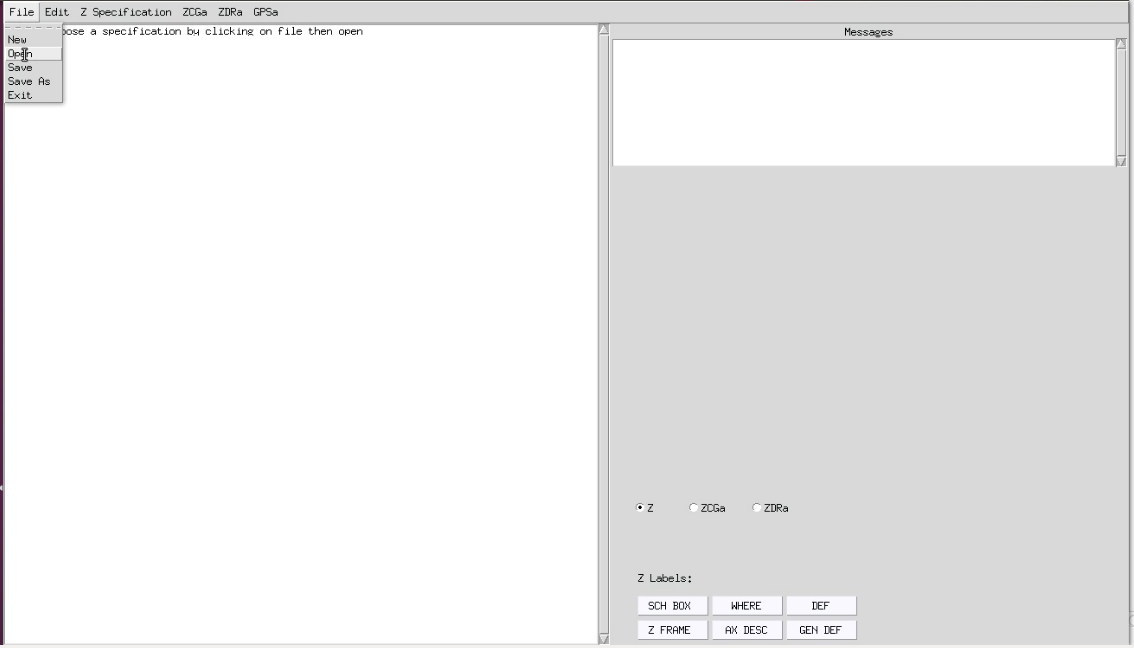
\includegraphics[scale=0.4]{Figures/Interface/openspec.png}
\caption{This figure shows the steps to open an existing specification to be imported into the user interface. \label{fig:openspec}}
\end{figure}

A pop up box appears asking the user to locate the specification they would like
to translate. An example of the pop up box is shown in figure
\ref{fig:choosespec}. 

\begin{figure}[H]
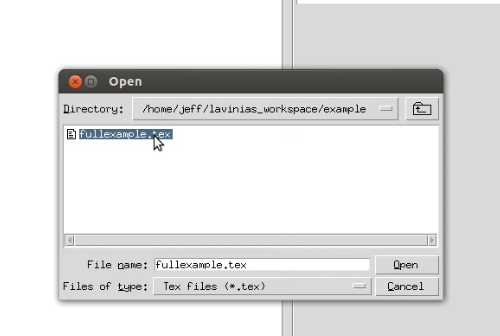
\includegraphics[scale=0.8]{Figures/Interface/choosespec.png}
\caption{This figure shows the pop  up  window that comes up when a user is asked which specification they wish to insert. In our example we would like to import a file named "fullexample.tex". \label{fig:choosespec}}
\end{figure}

Once a specification has been chosen then the specification should appear in the
panel on the left hand side. Figure \ref{fig:specinserted} shows an example of
this. Note that no messages appear yet in the messages box.

\begin{figure}[H]
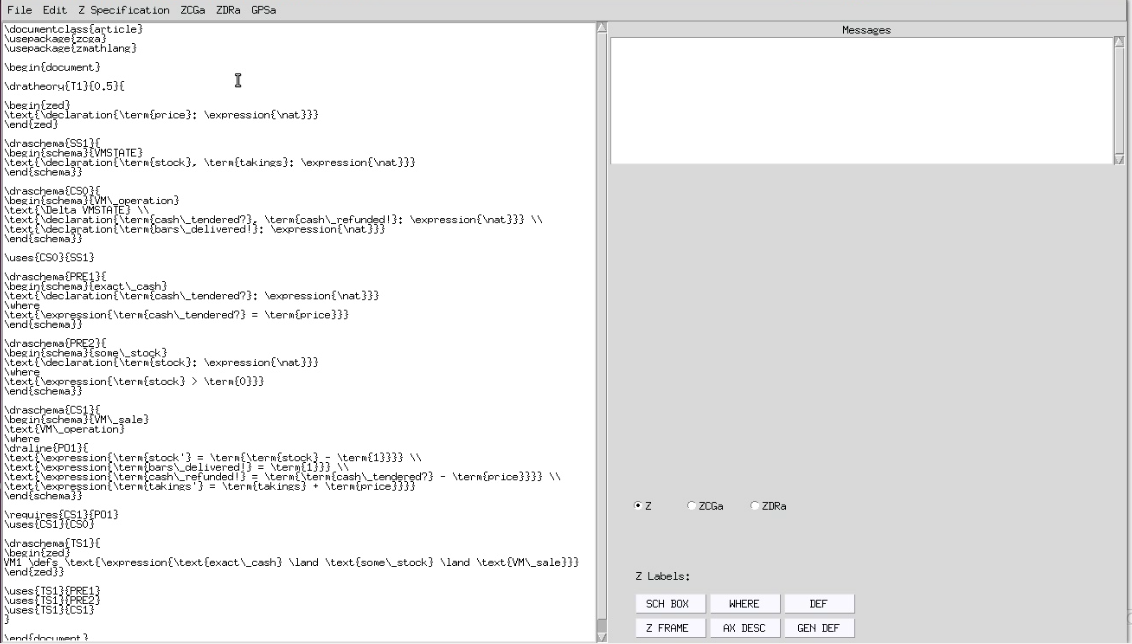
\includegraphics[scale=0.37]{Figures/Interface/specinserted.png}
\caption{This figure shows an imported in the user interface which is shown in the main panel on the left. \label{fig:specinserted}}
\end{figure}

\section{Checking ZCGa}
To then check for \gls{zcga} correctness the specification loaded into the
interface must be \gls{zcga} annotated.

\begin{figure}[H]
\centering
\begin{minipage}{0.45\textwidth}
\centering
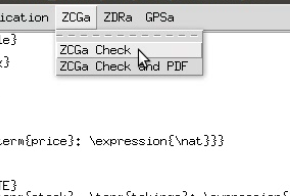
\includegraphics[scale=0.6]{Figures/Interface/zcgacheck.png}
\end{minipage}\hfill
\begin{minipage}{0.45\textwidth}
\centering
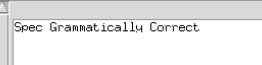
\includegraphics[scale=0.7]{Figures/Interface/zcgacorrect.png}
\end{minipage}
\caption{An example of how to check the specification for ZCGa correctness (left) and the message which appears when the specification is ZCGa correct (right).  \label{fig:zchecheck}}
\end{figure}

To check for \gls{zcga} correctness the user can click on the \emph{zcga} button
from the top menu and then click on \emph{Zcga Check}. If the specification is
grammatically correct then a message appears in the message box in the top right
of the interface (n see figure \ref{fig:zchecheck}).

\section{Checking ZDRa}

To check for \gls{zdra} correctness the specification loaded into the interface
must be labelled with \gls{zdra} annotations (this can be with or without
\gls{zcga} annotations).

\begin{figure}[H]
\centering
\begin{minipage}{0.4\textwidth}
\centering
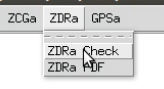
\includegraphics[scale=0.7]{Figures/Interface/zdracheck.png}
\end{minipage}\hfill
\begin{minipage}{0.6\textwidth}
\centering
\includegraphics[scale=0.6]{Figures/Interface/zdracorrect.png}
\end{minipage}
\caption{An example of how to check the specification for ZDRa correctness (left) and the message which appears when the specification is ZDRa correct.  \label{fig:zdracheck}}
\end{figure}

To check for \gls{zdra} correctness the user can click on the \emph{ZDRa} button
in the top menu of the interface and then on the \emph{Zdra Check} button. If
the specification is \gls{zdra} correct and the specification has been correctly
totalised then a message confirming this appears in the message box. Figure
\ref{fig:zdracheck} shows both of these actions.

\section{Skeletons}

The user may also want to create a general proof skeleton, Isabelle skeleton and
fill in the Isabelle skeleton using the Interface. This section explains how
this may be done.

\subsection{General Proof Skeleton}

To create a general proof skeleton from the users \gls{zdra} annotated and
correct specification. The user will need to input their specification into the
interface, check the specification for \gls{zdra} correctness then click on the
\emph{GPSa} button in the top menu and choose \emph{Proof Skeleton} from the
drop down menu. An example of this is shown in figure \ref{fig:gpsabutton}.

\begin{figure}[H]
\centering
\includegraphics[scale=0.8]{Figures/Interface/proofskeleton.png}
\caption{This part of the user interface shows the steps to create a general proof skeleton from the users loaded specification.. \label{fig:gpsabutton}}
\end{figure}

A new file should then appear in the same folder as your \texttt{Interface.py}
program (see figure \ref{fig:gpsadoc}).

\begin{figure}[H]
\centering
\includegraphics[scale=0.6]{Figures/Interface/skeletondoc.png}
\caption{A new file appears named skeleton in the same directory as the users specification. This is the automatically generated skeleton. \label{fig:gpsadoc}}
\end{figure}

The user may then open this file using an external text editor or they may view
it in the interface itself. When creating a general proof skeleton a message
appears in the Messages box saying \texttt{Skeleton Created}, a button also
appears underneath the message box saying \texttt{Show Skeleton} (see figure
\ref{fig:showskeleton}). By clicking on this new button the general proof
skeleton can be opened within the Interface. 

\subsection{Isabelle Skeleton}

After creating a general proof skeleton the user may want to take the
translation one step further and create an Isabelle proof skeleton. Again, to do
this the specification must be labelled with \gls{zdra} and be \gls{zdra}
correct. The user may then click on the \emph{GPSa} button in the top menu and
then the \emph{Isabelle Skeleton} button in the drop down menu as shown in
figure \ref{fig:converttoisa}.

\begin{figure}[H]
\centering
\includegraphics[scale=0.8]{Figures/Interface/isskeleton.png}
\caption{To create an Isabelle skeleton then `\textit{Isabelle Skeleton}' should be selected from the GPSa sub menu on the user interface. \label{fig:converttoisa}}
\end{figure}

If all is correct a message saying \texttt{Isabelle Skeleton Created} and a new
button should appear under the message box with the text \texttt{Show Isabelle
Skeleton} as seen in figure \ref{fig:showskeleton}. A new file will be produced
and automatically saved in the same directory as the interface with a
\emph{.thy} extension.

\begin{figure}[H]
\centering
\includegraphics[scale=0.7]{Figures/Interface/showsaskeleton.png}
\caption{New buttons which appear on the right hand side of the interface if the user chooses to create a general proof skeleton or an Isabelle skeleton. \label{fig:showskeleton}}
\end{figure}

The user may then open the Isabelle skeleton using an external text editor such
as Jedit or Isabelle itself or they may choose to open the Isabelle Skeleton
within the interface by clicking on the \texttt{Show Isabelle Skeleton Button}.
An example of a pop-up window showing the Isabelle skeleton in the user
interface can be seen in figure \ref{fig:isaskelpopup}.

\begin{figure}[H]
\centering
\includegraphics[scale=0.5]{Figures/Interface/isaskelpopup.png}
\caption{By clicking `\textit{Show Isabelle skeleton}' a box will be displayed in the user interface showing the isabelle skeleton. \label{fig:isaskelpopup}}
\end{figure}

The user may even wish to go as far as filling in the Isabelle skeleton. To do
this the Isabelle skeleton will need to be created first and the specification
loaded into the interface must also be annotated with \gls{zcga}. The user can
then click on \texttt{GPSa} in the top level menu and then
\texttt{FillInIsaSkeleton} (see figure \ref{fig:fillinisaskel}). If the skeleton
is not in the same directory as the interface or has been renamed then the
interface will ask for the user to locate the Isabelle skeleton in a similar way
to opening a specification (figure \ref{fig:choosespec}).

\begin{figure}[H]
\centering
\includegraphics[scale=0.7]{Figures/Interface/fillinisaskel.png}
\caption{This figure shows the steps to automatically fill in the Isabelle skeleton. The user can choose the `\textit{FillInIsaSkeleton}' from the GPSa sub menu. \label{fig:fillinisaskel}}
\end{figure}

The user may then wish to open the filled-in isabelle skeleton externally or in
the interface the same was as they opened the skeleton in the previous step.

\section{Output messages which could occur}

Sometimes there is an error in any of the actions previously described in this
chapter. The message box not only tells the user what has been successful but it
also gives the user information if there has been some error in the action they
were trying. Table \ref{tab:uimessages} shows all the possible messages which
can appear in the message box along with an explanation about the message.

{\def\arraystretch{0.5}\tabcolsep=0.5pt
\begin{longtable}[H]{|l | l |}
\hline
\textbf{Text in message box} & \textbf{Explanation} \\
\hline
\hline
\verb|Specification Correctly| & All preconditions in the specification\\
\verb|Totalised| & have a totalising condition  \\
\hline
\verb|Warning! Specification not| & Not all preconditions have an alternative \\
\verb|correctly totalised| & output (skeleton can still be created) \\
& \textit{(see chapter \ref{chap:zdra})} \\
\hline
\verb|Specification is Rhetorically| & Specification is ZDRa correct \\
\verb|Correct| & \textit{(see chapter \ref{chap:zdra})} \\
\hline
\verb|Skeleton Created| & General proof skeleton has been successfully \\
& created \\
\hline
\verb|Isabelle Skeleton Created| & Isabelle skeleton has been successfully
created \\
\hline
\verb|Isabelle Skeleton successfully| & Isabelle proof skeleton has been \\
\verb|filled in| & filled in using ZCGa text \\
\hline
\verb|Please convert specification| & Covert the specification into an  \\
\verb|into Isabelle Skeleton first| & Isabelle skeleton first before filling it
in \\
& \textit{(see chapter \ref{ch:skeletons})} \\
\hline
\verb|Please select your isabelle| & Please locate the Isabelle skeleton\\
\verb|skeleton:| & which you wish to be filled in \textit{(see chapter
\ref{ch:skeletons})}\\
\hline
\verb|Please convert specification| & Can not find the \\
\verb|into GPSa first| & general proof skeleton \textit{(see chapter
\ref{ch:skeletons})}\\
\hline
\verb|Loops in reasoning| & Specification is not ZDRa correct \\
\verb|Can not create Skeleton| & and the skeleton can not be created \\
& \textit{(see chapter \ref{ch:zdra})}\\
\hline
\verb|Spec Grammatically Correct| & The specification has passed ZCGa checker \\
\hline
\verb|Spec Grammatically Incorrect|& The specification has failed ZCGa
correctness\\
\verb|Number of errors: 2| & and has 2 errors \textit{(see chapter
\ref{chap:zcga})}\\
\hline 

\\ \caption{Messages which could appear in the user interface and their meanings.}
\label{tab:uimessages}
\end{longtable}
}

\section{Conclusion}
This chapter has described how a user of the \gls{zmath} framework can use the
implemented user interface to assist them with checking for grammatical and
rhetorical correctness. The user interface also gives a clear and easy way to
translate the specification into a general proof skeleton, Isabelle skeleton and
filling in the Isabelle skeleton without using the user unfriendly terminal. The
interface also allows the user to view the documents automatically produced from
the annotated specification.
%\chapter{From raw specification to fully proven spec: A full example}
\label{ch:fullexample}
%Chapter 9

In this chapter we take a system specification through all the steps of
\gls{zmath} to demonstrate how we can get from a raw specification to a full
proof. We have added commentary throughout so the reader can understand how we
can get from one step to another. We have added figures and screenshots of each
step of the \gls{zmath} framework.

\section{ModuleReg Example}
We have chosen to demonstrate the Modulereg specification from start to finish
using the steps of \gls{zmath} as the modulereg specification contains 2 state
invariants which means we can demonstrate \gls{zmath} automatically generating
the lemmas to prove. The  Modulereg specification is also a good size to fit
onto one page to make it easy for the reader.

\subsection{Step 0\\Raw Specification}
We take the raw specification ModuleReg \cite{essenceofz}, which displays students
taking modules in a school environment (shown in figure \ref{fig:rawschema}) The
output for the specification can be seen in figure \ref{fig:rawschemaout}. The
full proof for the ModuleReg specification can be found in \ref{app:moduleregfullproof}.

\begin{figure}[H]
\vspace{-0.2in}
\centering
\begin{minipage}{0.45\textwidth}
\centering
\begin{tiny}
\begin{BVerbatim}
\documentclass{article}
\usepackage{zmathlang}
\begin{document}

\begin{zed}
[PERSON, MODULE]
\end{zed}

\begin{schema}{ModuleReg}
students: \power PERSON \\
degModules: \power MODULE \\
taking: PERSON \rel MODULE
\where
\dom taking \subseteq students \\
\ran taking \subseteq degModules
\end{schema}

\begin{schema}{AddStudent}
\Delta ModuleReg \\
p?: PERSON \\
\where
p? \notin students \\
students' = students \cup \{p?\} \\
degModules' = degModules \\
taking' = taking
\end{schema}

\begin{schema}{RegForModule}
\Delta ModuleReg \\
p?: PERSON \\
m?: MODULE
\where
p? \in students \\
m? \in degModules \\
p? \mapsto m? \notin taking \\
taking' = taking \cup \{p? \mapsto m?\} \\
students' = students \\
degModules' = degModules
\end{schema}
\end{document}
\end{BVerbatim}
\end{tiny}
%\vspace{-0.2in}
\caption{Part of the raw schema.\label{fig:rawschema}}
%\vspace{-0.2in}
\end{minipage}\hfill
\begin{minipage}{0.45\textwidth}
\centering
%\fbox{\includegraphics[trim=5cm 13cm 6 11cm]{examples/modulereg/0.pdf}}
\includegraphics[clip, trim=5cm 11.5cm 10cm 5.5cm, width=1.00\textwidth]{examples/modulereg/0.pdf}
%\includegraphics[scale=0.4]{Figures/fullexample/raw.png}
\vspace{-0.2in}
\caption{Part of a raw specification output. \label{fig:rawschemaout}}
\vspace{-0.2in}
\end{minipage}
\end{figure}


\subsection{Step 1\\ZCGa}

The user then goes to label the raw specification with the \gls{zcga} labels.
The labelled specification can be seen in figure \ref{fig:zcgaschema}. The words
highlighted in {\color{red}red} are the \gls{zcga} annotations done by the user
and the black text is the existing specification. The output from figure \ref{fig:zcgaschema}
is shown in figure \ref{fig:zcgaschemaout}.

\begin{figure}[H]
\centering
\begin{minipage}{0.45\textwidth}
\centering
\begin{tiny}
\begin{BVerbatim}[commandchars=+\[\]]
\documentclass{article}
\usepackage{zmathlang}
\begin{document}
\begin{zed}
[+color[red]\set{]PERSON[+color[red]}], [+color[red]\set{]MODULE[+color[red]}]
\end{zed}
\begin{schema}{ModuleReg}
[+color[red]\text{\declaration{\set{]students[+color[red]}]:[+color[red]\expression{]\power
PERSON[+color[red]}}}]\\
[+color[red]\text{\declaration{\set{]degModules[+color[red]}]:[+color[red]\expression{]\power
MODULE[+color[red]}}}]\\
[+color[red]\text{\declaration{\set{]taking[+color[red]}]:[+color[red]\expression{]PERSON
\rel MODULE[+color[red]}}}]
\where
[+color[red]\text{\expression{\set{]\dom [+color[red]\set{]taking[+color[red]}}]
\subseteq [+color[red]\set{]students[+color[red]}}}]\\
[+color[red]\text{\expression{\set{]\ran [+color[red]\set{]taking[+color[red]}}]
\subseteq [+color[red]\set{]degModules[+color[red]}}}]
\end{schema}
\begin{schema}{AddStudent}
[+color[red]\text{]\Delta ModuleReg[+color[red]}]\\
[+color[red]\text{\declaration{\term{]p?[+color[red]}]:[+color[red]\expression{]PERSON[+color[red]}}}]\\
\where
[+color[red]\text{\expression{\term{]p?[+color[red]}] \notin
[+color[red]\set{]students[+color[red]}}}]\\
[+color[red]\text{\expression{\set{]students'[+color[red]}] =
[+color[red]\set{\set{]students[+color[red]}] \cup
[+color[red]\set{]\{[+color[red]\term{]p?[+color[red]}]\}[+color[red]}}}}]\\
[+color[red]\text{\expression{\set{]degModules'[+color[red]}] =
[+color[red]\set{]degModules[+color[red]}}}]\\
[+color[red]\text{\expression{\set{]taking'[+color[red]}] =
[+color[red]\set{]taking[+color[red]}}}]
\end{schema}
\begin{schema}{RegForModule}
[+color[red]\text{]\Delta ModuleReg[+color[red]}]\\
[+color[red]\text{\declaration{\term{]p?[+color[red]}]:
[+color[red]\expression{]PERSON[+color[red]}}}]\\
[+color[red]\text{\declaration{\term{]m?[+color[red]}]:
[+color[red]\expression{]MODULE[+color[red]}}}]
\where
[+color[red]\text{\expression{\term{]p?[+color[red]}] \in
[+color[red]\set{]students[+color[red]}}}]\\
[+color[red]\text{\expression{\term{]m?[+color[red]}] \in
[+color[red]\set{]degModules[+color[red]}}}]\\
[+color[red]\text{\expression{\term{\term{]p?[+color[red]}] \mapsto
[+color[red]\term{]m?[+color[red]}}] \notin
[+color[red]\set{]taking[+color[red]}}}]\\
[+color[red]\text{\expression{\set{]taking'[+color[red]}] =
[+color[red]\set{\set{]taking[+color[red]}] \cup
[+color[red]\set{]\{[+color[red]\term{\term{]p?[+color[red]}] \mapsto
[+color[red]\term{]m?[+color[red]}}]\}[+color[red]}}}}]\\
[+color[red]\text{\expression{\set{]students'[+color[red]}] =
[+color[red]\set{]students[+color[red]}}}]\\
[+color[red]\text{\expression{\set{]degModules'[+color[red]}] =
[+color[red]\set{]degModules[+color[red]}}}]
\end{schema}
\end{document}
\end{BVerbatim}
\end{tiny}
%\vspace{-0.2in}
\caption{Part of the raw schema.\label{fig:zcgaschema}}
%\vspace{-0.2in}
\end{minipage}\hfill
\begin{minipage}{0.45\textwidth}
\centering
\centering
%\includegraphics[scale=0.3, clip, trim=5.5cm 8cm 9.5cm 4cm, width=1.00\textwidth]{Figures/fullexample/1.jpg}
%\includegraphics[scale=0.3, clip, trim=5.5cm 13cm 8.5cm 4cm, width=1.00\textwidth]{Figures/fullexample/2.jpg}
\includegraphics[width=7cm]{Figures/fullexample/1a.jpg}
\includegraphics[width=7cm]{Figures/fullexample/2b.jpg}

\caption{Part of a ZCGa labelled specification output. \label{fig:zcgaschemaout}}
\end{minipage}
\end{figure}

After annotating the text, we run it through the \gls{zcga} correctness checker. Figure
\ref{fig:zcgacorrect} shows the message which appears when the annotated
specification has been checked. 

\begin{figure}[H]
\centering
\includegraphics[scale=0.4]{Figures/fullexample/zcgacorrect.png}
\caption{Message which appears after running the ZCGa checker on our example. \label{fig:zcgacorrect}}
\end{figure}

\subsection{Step 2\\ZDRa}

Next the user can add \gls{zdra} relations to chunk parts of the specification
together and add relations to them. Figure \ref{fig:zdrazcgaAno} shows our
example labelled in \gls{zdra} annotations (in blue), the \gls{zcga} annotations
are in grey and existing specification in black. Figure \ref{fig:zdrazcgaout}
shows the compiled result.

\begin{figure}[H]
\vspace{-0.2in}
\centering
\begin{minipage}{0.45\textwidth}
\centering
\begin{tiny}
\begin{BVerbatim}[commandchars=+\[\]]
\documentclass{article}
\usepackage{zmathlang}
\begin{document}

[+color[blue]\dratheory{T1}{0.5}{]
\begin{zed}
[+color[gray]\set{]PERSON[+color[gray]}],
[+color[gray]\set{]MODULE[+color[gray]}]
\end{zed}

[+color[blue]\draschema{SS1}{]
\begin{schema}{ModuleReg}
[+color[gray]\text{\declaration{\set{]students[+color[gray]}]:[+color[gray]\expression{]\power
PERSON[+color[gray]}}}]\\
[+color[gray]\text{\declaration{\set{]degModules[+color[gray]}]:[+color[gray]\expression{]\power
MODULE[+color[gray]}}}]\\
[+color[gray]\text{\declaration{\set{]taking[+color[gray]}]:[+color[gray]\expression{]PERSON
\rel MODULE[+color[gray]}}}]
\where
[+color[blue]\draline{SI1}{] [+color[gray]\text{\expression{\set{]\dom
[+color[gray]\set{]taking[+color[gray]}}] \subseteq
[+color[gray]\set{]students[+color[gray]}}}]\\
[+color[gray]\text{\expression{\set{]\ran
[+color[gray]\set{]taking[+color[gray]}}] \subseteq
[+color[gray]\set{]degModules[+color[gray]}}}][+color[blue]}]
\end{schema}[+color[blue]}]

[+color[blue]\requires{SS1}{SI1}]

[+color[blue]\draschema{CS1}{]
\begin{schema}{AddStudent}
[+color[gray]\text{]\Delta ModuleReg[+color[gray]}]\\
[+color[gray]\text{\declaration{\term{]p?[+color[gray]}]:[+color[gray]\expression{]PERSON[+color[gray]}}}]\\
\where
[+color[blue]\draline{PRE1}{]
[+color[gray]\text{\expression{\term{]p?[+color[gray]}] \notin
[+color[gray]\set{]students[+color[gray]}}}][+color[blue]}]\\
[+color[blue]\draline{PO1}{]
[+color[gray]\text{\expression{\set{]students'[+color[gray]}] =
[+color[gray]\set{\set{]students[+color[gray]}] \cup
[+color[gray]\set{]\{[+color[gray]\term{]p?[+color[gray]}]\}[+color[gray]}}}}]\\
[+color[gray]\text{\expression{\set{]degModules'[+color[gray]}] =
[+color[gray]\set{]degModules[+color[gray]}}}]\\
[+color[gray]\text{\expression{\set{]taking'[+color[gray]}] =
[+color[gray]\set{]taking[+color[gray]}}}][+color[blue]}]
\end{schema}[+color[blue]}]

[+color[blue]\requires{CS1}{PRE1}] [+color[blue]\allows{PRE1}{PO1}]
[+color[blue]\uses{CS1}{SS1}]

[+color[blue]\draschema{CS2}{]
\begin{schema}{RegForModule}
[+color[gray]\text{]\Delta ModuleReg[+color[gray]}]\\
[+color[gray]\text{\declaration{\term{]p?[+color[gray]}]:
[+color[gray]\expression{]PERSON[+color[gray]}}}]\\
[+color[gray]\text{\declaration{\term{]m?[+color[gray]}]:
[+color[gray]\expression{]MODULE[+color[gray]}}}]
\where

\end{document}
\end{BVerbatim}
\end{tiny}
%\vspace{-0.18in}
\caption{An example of a specification labelled in \gls{zcga} and \gls{zdra}.\label{fig:zdrazcgaAno}}
%\vspace{-0.2in}
\end{minipage}\hfill
\begin{minipage}{0.45\textwidth}
\centering
\begin{tiny}
\begin{BVerbatim}[commandchars=+\[\]]
[+color[blue]\draline{PRE2}{]
[+color[gray]\text{\expression{\term{]p?[+color[gray]}] \in
[+color[gray]\set{]students[+color[gray]}}}]\\
[+color[gray]\text{\expression{\term{]m?[+color[gray]}] \in
[+color[gray]\set{]degModules[+color[gray]}}}]\\
[+color[gray]\text{\expression{\term{\term{]p?[+color[gray]}] \mapsto
[+color[gray]\term{]m?[+color[gray]}}] \notin
[+color[gray]\set{]taking[+color[gray]}}}][+color[blue]}]\\
[+color[blue]\draline{PO2}{]
[+color[gray]\text{\expression{\set{]taking'[+color[gray]}] =
[+color[gray]\set{\set{]taking[+color[gray]}] \cup
[+color[gray]\set{]\{[+color[gray]\term{\term{]p?[+color[gray]}] \mapsto
[+color[gray]\term{]m?[+color[gray]}}]\}[+color[gray]}}}}]\\
[+color[gray]\text{\expression{\set{]students'[+color[gray]}] =
[+color[gray]\set{]students[+color[gray]}}}]\\
[+color[gray]\text{\expression{\set{]degModules'[+color[gray]}] =
[+color[gray]\set{]degModules[+color[gray]}}}][+color[blue]}]
\end{schema}[+color[blue]}] [+color[blue]}]


\end{BVerbatim}
\end{tiny}
%\includegraphics[scale=1, clip, trim=2cm 3cm 2cm 3cm, width=1.00\textwidth]{Figures/fullexample/1n2.pdf}
\includegraphics[scale=0.75]{Figures/fullexample/1n2.jpg}
%\vspace{-0.18in}
\caption{An example of a specification output labelled in \gls{zcga} and \gls{zdra}.\label{fig:zdrazcgaout}}
%\vspace{-0.2in}
\end{minipage}
\end{figure}

After annotating our example in \gls{zdra} labels we can then run our
specification through the \gls{zdra} checker. Figure \ref{fig:zdracorrect} shows
the message which appears after we check our example with \gls{zdra}.

\begin{figure}[H]
\centering
\includegraphics[scale=0.3]{Figures/fullexample/zdracorrect.png}
\caption{Message which appears after running the ZDRa checker on our example. \label{fig:zdracorrect}}
\end{figure}

\subsection{Step 2.5\\Graphs}

Since the example is \gls{zdra} correct the two graphs shown in figures
\ref{fig:depexample} and \ref{fig:gotoexample} are automatically produced and
saved on the users computer.

\begin{figure}[H]
\centering
\includegraphics[scale=0.7]{Figures/fullexample/dp_fullexample.png}
\caption{Dependency graph automatically generated from the ZDRa for our example. \label{fig:depexample}}
\end{figure}

\begin{figure}[H]
\centering
\includegraphics[scale=0.7]{Figures/fullexample/goto_fullexample.jpg}
\caption{GoTo graph automatically generated from the ZDRa for our example. \label{fig:gotoexample}}
\end{figure}

\subsection{Skeletons}

The skeletons can be automatically generated if the specification passes the
\gls{zcga} and \gls{zdra} check.

\subsubsection{Step 3\\General Proof Skeleton}

We can generate a general proof skeleton which prints out the \gls{zdra} name
and the instances they should be converted to when inputting into any theorem
prover. If the specification is \gls{zdra} correct we can then generate the
\gls{gpsa} by clicking on the \gls{gpsa} menu in the interface (figure
\ref{fig:gpsabutton}).

\begin{figure}[H]
\centering
\includegraphics[scale=1]{Figures/fullexample/proofskelbutton.png}
\caption{The GPSa button allows the user to generate the general proof skeleton. \label{fig:gpsabutton}}
\end{figure}

The GPSa can be created after a specification has been annotated with ZDRa. The GPSa is what orders the specification 
logically to put into a theorem prover. Steps 4, 5 and 6 will need to be created after the GPSa. Step 4 will use the skeleton 
created in step 3 and ZCGa annotations created in step 2 to create the Isabelle skeleton. The Isabelle skeleton in
step 4 requires ZCGa annotations and the GPSa to be complete. Without the GPSa, the logical order of the specification may not be correct
e.g. there may be some changeSchemas used which haven't been created yet. Without the ZCGa, some variables may be used which haven't been 
declared and therefore will not parse through Isabelle.

Figure \ref{fig:gpsaFullexample} shows the general proof skeleton which was
generated for our example. Note all instances but the last 2 are actual
instances labelled by the user. Since there are 2 instances where there could be
a change in state (CS1 and CS2) then there are 2 proof obligations added to the
\gls{gpsa} (L1\_CS2 and L2\_CS1).

\begin{figure}[H]
\centering
\begin{scriptsize}
\begin{BVerbatim}
stateSchema SS1
stateInvariants SI1
changeSchema CS2
precondition PRE2
changeSchema CS1
precondition PRE1
postcondition PO2
postcondition PO1
lemma L1_(CS2)
lemmaL2_(CS1) 
\end{BVerbatim}
\end{scriptsize}
\caption{General proof skeleton. \label{fig:gpsaFullexample}}
\end{figure}

\subsubsection{Step 4\\Isabelle Skeleton}

From \gls{gpsa}, the ZMathLang program can automatically generate an Isabelle
Skeleton. The user can do this by clicking on the \gls{gpsa} menu on the
interface then clicking `\texttt{Isabelle Skeleton}' shown in figure
\ref{fig:isabutton}.

\begin{figure}[H]
\centering
\includegraphics[scale=1]{Figures/fullexample/isaskelbutton.png}
\caption{The Isabelle skeleton button allows the user to generate an Isabelle skeleton of their specification. \label{fig:isabutton}}
\end{figure}

 The Isabelle skeleton consists of the information generated in the general
 proof skeleton along with the environment to begin an Isabelle theory. It
 contains comments in between \verb|(* .. *)| parenthesis to show the parts which
 need to be filled in either by using the \gls{zcga} document or by the user.
 Figure \ref{fig:isaFullexample} shows the automatically generated Isabelle
 skeleton for our \texttt{modulereg} example.

\begin{figure}[H]
\centering
\begin{scriptsize}
\begin{BVerbatim}
theory gpsaModuleReg
imports Main begin (*DATATYPES*)
record SS1 = (*DECLARATIONS*)
locale 1n2 = fixes (*GLOBAL DECLARATIONS*)
assumes SI1 begin definition CS2 ::
"(*CS2_TYPES*) => bool"
where
"CS2 (*CS2_VARIABLES*) == (PRE2) \<and> (PO2)"
definition CS1 :: "(*CS1_TYPES*) => bool"
where
"CS1 (*CS1_VARIABLES*) == (PRE1) \<and> (PO1)"

lemma CS2_L1: "(\<exists> (*CS2_VARIABLESANDTYPES*).
(PRE2) \<and> (PO2) \<longrightarrow> 
(SI1) \<and> (SI1'))" 
sorry 
lemma CS1_L2: "(\<exists> (*CS1_VARIABLESANDTYPES*).
(PRE1) \<and> (PO1) \<longrightarrow> 
((SI1) \<and> (SI1')))" sorry 
end
end
\end{BVerbatim}
\end{scriptsize}
\caption{Isabelle proof skeleton. \label{fig:isaFullexample}}
\end{figure}

\subsubsection{Step 5\\Isabelle Skeleton Filled in}

Using the \gls{zcga} annotated document and the Isabelle skeleton described in
the previous section. The user can then automatically fill in the missing
information which is needed between the comment parenthesis \verb|(* ...*)|.
This is the final step which is automated by the program and the user can click
on the \gls{gpsa} button on the main menu bar in the interface and then click on
`\texttt{FillInIsa Skeleton}' in the sub menu (shown in figure
\ref{fig:fillinisa}).

\begin{figure}[H]
\centering
\includegraphics[scale=1]{Figures/fullexample/fillinisabutton.png}
\caption{The "FillInIsa Skeleton" button allows the user to fill in the skeleton they previously created. \label{fig:fillinisa}}
\end{figure}

Figure \ref{fig:fillinFullexample} shows our example with a filled in Isabelle
skeleton. It is important to note that the program also changes some of the
syntax from \LaTeX{} to Isabelle so that it is fully parsable by Isabelle.
We have used the rules described in section \ref{sec:zcga2fillin} to fill in the Isabelle
 skeleton with the ZCGa annotations.

\begin{figure}[H]
\centering
\begin{minipage}{0.45\textwidth}
\centering
\begin{scriptsize}
\begin{BVerbatim}
theory gpsaModuleReg imports Main 

begin typedecl PERSON typedecl MODULE

record ModuleReg = STUDENTS :: " PERSON set"
DEGMODULES :: " MODULE set" TAKING
:: "(PERSON * MODULE) set"

locale gpsaModuleReg = fixes students :: 
" PERSON set" and degModules :: "
MODULE set" and taking :: "(PERSON * MODULE) set"
 assumes "Domain taking
\<subseteq> students" and 
"Range taking \<subseteq> degModules" begin

definition RegForModule :: 
"ModuleReg \<Rightarrow> ModuleReg \<Rightarrow>
PERSON \<Rightarrow> MODULE => MODULE set 
\<Rightarrow> PERSON set \<Rightarrow>
(PERSON * MODULE) set \<Rightarrow> bool" where 
"RegForModule modulereg
modulereg' p m degModules' students' taking' == 
(p \<in> students) \<and> (m
\<in> degModules) \<and> ((p, m) \<notin> taking) 
\<and> (taking' = taking\<union> {(p, m)}) \<and> 
(students' = students) 
\<and> (degModules' =degModules)"

definition AddStudent :: "ModuleReg \<Rightarrow> 
ModuleReg => PERSON
\<Rightarrow>  MODULE set \<Rightarrow> PERSON set 
\<Rightarrow> (PERSON *
MODULE) set \<Rightarrow> bool" where "AddStudent 
modulereg modulereg' p
degModules' students' taking' == ((p \<notin> students) 
\<and> (students' =
students \<union> {(p)}) 
\end{BVerbatim}
\end{scriptsize}
\end{minipage}\hfill
\begin{minipage}{0.45\textwidth}
\begin{scriptsize}
\begin{BVerbatim}
\<and> (degModules' = degModules) \<and> 
(taking' = taking))"

lemma RegForModule_L1: 
"(\<exists> degModules:: MODULE set. 
\<exists> students
:: PERSON set. \<exists> taking :: 
(PERSON * MODULE) set. \<exists> p :: PERSON.
\<exists> degModules':: MODULE set. 
\<exists> students' :: PERSON set. \<exists>
taking' :: (PERSON * MODULE) set. 
\<exists> m :: MODULE. ((p \<in> students)
\<and> (m \<in> degModules) \<and> ((p, m) 
\<notin> taking) \<and> (taking' =
taking \<union> {(p, m)}) \<and> 
(students' = students) 
\<and> (degModules' =
degModules)) \<longrightarrow> ((Domain taking 
\<subseteq> students) \<and>
(Range taking \<subseteq> degModules) \<and> 
(Domain taking' \<subseteq>
students') \<and> (Range taking' 
\<subseteq> degModules')))" sorry

lemma AddStudent_L2: 
"(\<exists> degModules:: MODULE set. 
\<exists> students ::
PERSON set. \<exists> taking :: 
(PERSON * MODULE) set. 
\<exists> p :: PERSON.
\<exists> degModules':: MODULE set. 
\<exists> students' :: PERSON set. \<exists>
taking' :: (PERSON * MODULE) set. 
( (students' = students \<union> {(p)}) \<and>
(degModules' = degModules) \<and> 
(taking' = taking)) 
\<longrightarrow ((Domain
taking \<subseteq> students) \<and> 
(Range taking \<subseteq> degModules) \<and>
(Domain taking' \<subseteq> students') 
\<and> (Range taking' \<subseteq>
degModules')))" sorry end end
\end{BVerbatim}
\end{scriptsize}
\end{minipage}
\caption{Filled In proof skeleton. \label{fig:fillinFullexample}}
\end{figure}

Figure \ref{fig:fillinFullexample} shows the original specification we started
with in step 0 in Isabelle syntax. It is important to the reader to note that we
have come this far without the user knowing any Isabelle at all. In our example
we have 2 existing lemma's to prove to check the consistency of the
specification. That is the state before \texttt{RegForModule} (PRE2), \emph{and}
the state after \texttt{RegforModule} (PO2), \emph{implies}
\texttt{stateInvariants} (SI1), \emph{and} the \texttt{stateInvariants'} (SI1')
is true. So the precondition and postcondition imply that the stateInvariants
and stateInvariants prime hold. The same goes for the \texttt{AddStudent}
operation. When the skeleton is filled in, \gls{zmath} is unable to prove the
lemma's automatically and it is up to the user to do this (explained in the next
section). However at this stage \gls{zmath} puts the Isar command
`\texttt{sorry}' as to ignore the lemma and act as if it was proven.

In this case the new "Lemmas" are added to the end of the specification at random.
For this specification it doesn't matter which lemma comes first (RegForModule\_L1 or AddStudent\_L2)
as the schemas \texttt{RegForModule} and \texttt{AddStudent} are independent of
each other
and one does not `\textit{use}' the other. If we did have a changeSchema which did use another changeSchema
then this would have to be annotated in the ZDRa and therefore the order would matter when the lemmas are produced.


\subsection{Step 6\\Full Proof}

The next part is to prove any existing lemmas from the filled in Isabelle
Skeleton or add new lemma's to prove safety properties about the specification.
However, this final stage is difficult to automate with \gls{zmath} as everyone
has different properties they wish to prove and all specification are different
themselves. So the final step will need some theorem prover knowledge, but not
as much as translating the specification and proving it in one step as the
specification is already put into the theorem prover syntax. In this case the
user may wish to use theorem prover tools which already exist such as
Sledgehammer \cite{sledgehammer} to help them prove the properties. An example
is shown in figure \ref{fig:propertyproof} the proof obligations being proven by
hand for the \texttt{modulereg} specification.

\begin{figure}[H]
\centering
\begin{minipage}{0.45\textwidth}
\centering
\begin{scriptsize}
 \begin{BVerbatim}[commandchars=+\[\]] 
lemma RegForModule_L1: "(\<exists>
degModules:: MODULE set. \<exists> students ::
 PERSON set. \<exists> taking ::
(PERSON * MODULE) set. \<exists> p :: PERSON. 
\<exists> degModules':: MODULE
set. \<exists> students' :: PERSON set. 
\<exists> taking' :: (PERSON * MODULE)
set. \<exists> m :: MODULE. ((p \<in> students) 
\<and> (m \<in> degModules)
\<and> ((p, m) \<notin> taking) \<and> 
(taking' = taking \<union> {(p, m)})
\<and> (students' = students) \<and> 
(degModules' = degModules))
\<longrightarrow> ((Domain taking 
\<subseteq> students)  \<and> (Range taking
\<subseteq> degModules) \<and> (Domain taking' 
\<subseteq> students') \<and>
(Range taking' \<subseteq> degModules')))"

[+color[red]by (smt Domain_empty Domain_insert] 
[+color[red]Range.intros
Range_empty Range_insert]
\end{BVerbatim}
\end{scriptsize}
\end{minipage}\hfill
\begin{minipage}{0.45\textwidth}
\begin{scriptsize}
\begin{BVerbatim}[commandchars=+\[\]]
[+color[red]Un_empty Un_insert_right empty_iff] 
[+color[red]empty_subsetI 
 empty_subsetI insert_mono]
[+color[red]insert_mono singletonI singletonI ]
[+color[red]singleton_insert_inj_eq' ]
[+color[red]singleton_insert_inj_eq')]

lemma AddStudent_L2: 
"(\<exists> degModules:: MODULE set. 
\<exists> students :: PERSON set. 
\<exists> taking :: (PERSON * MODULE) set. 
\<exists> p :: PERSON.
\<exists> degModules':: MODULE set. 
\<exists> students' :: PERSON set. \<exists>
taking' :: (PERSON * MODULE) set. 
((students' = students \<union> {(p)}) \<and>
(degModules' = degModules) \<and> 
(taking' = taking))
 \<longrightarrow> ((Domain
taking \<subseteq> students) \<and> 
(Range taking \<subseteq> degModules) \<and>
(Domain taking' \<subseteq> students') \<and> 
(Range taking' \<subseteq>
degModules')))"

[+color[red]by blast]
\end{BVerbatim}
\end{scriptsize}
\end{minipage}
\caption{An example of a property and it's proof for the Module Reg example. \label{fig:propertyproof}}
\end{figure}

Figure \ref{fig:propertyproof} shows how the lemmas are automatically generated from
the \gls{zdra} annotated specification (black) and the user input needed to
prove this lemma (red). Notice that the user has deleted the word
"\texttt{sorry}" which would have automatically come after the lemma.
The user has completed this proof by using techniques written in Isabelle, there are some forms of 
help by automatically solving proofs using the "sledgehammer" and "smt" provers which is what the 
user used to help solve these proofs.
Proofs can be completed in a variety of different ways and there are so many different strategies 
to complete a single proof. Automatically solving proofs can be a whole research area in itself.
More information on proving these lemmas can be found in the Isabelle Manual
\cite{isabelle} and is beyond the scope of this thesis.

We know that the Isabelle skeleton is now correct as it can be parsed through the 
Isabelle theorem prover with no errors.
All variables have been declared before they are used in Isabelle and all the ZCGa names
have been translated back to the original names used in the Z Specification.

\section{Autopilot Specification}
Here, we show a section of an autopilot specification \cite{Butler96} in natural
language, which describes
the control of an aircraft without constant manual input by the human pilot.

\subsection{Step 0\\Raw Specification}

 \begin{figure}[H]
     \vspace{-0.2in}
     \centering
     \begin{minipage}{0.45\textwidth}
     \centering
     \begin{tiny}
     \begin{BVerbatim}
\documentclass{article}
\begin{document}        
\begin{enumerate}
\item The mode-control panel contains four buttons
 for selecting modes and three displays for
dialing in or displaying values. The system supports
 the following four modes:
           
\begin{itemize}
\item attitude control wheel steering (att\_cws)
\item flight path angle selected (fpa\_sel)
\item altitude engage (alt\_eng)
\item calibrated air speed (cas\_eng)
\end{itemize}
          
\begin{zed}
events ::= press\_att\_cws |  press\_cas\_eng | 
press\_alt\_eng | \\
press\_fpa\_sel
\end{zed}
          
Only one of the first three modes can be engaged at 
any time. However, the cas\_eng mode
can be engaged at the same time as any of the other 
modes. The pilot engages a mode by pressing
the corresponding button on the panel. One of the 
three modes, att\_cws, fpa\_sel, or alz\_eng,
should be engaged at all times. Engaging any of the
 first three modes will automatically cause the
other two to be disengaged since only one of these
 three modes can be engaged at a time.
           
\begin{zed}
mode\_status ::= off | engaged
\end{zed}
      
\begin{schema}{off\_eng}
mode: mode\_status
\where
mode = off \lor mode = engaged
\end{schema}
           
\begin{schema}{AutoPilot}
att\_cws: mode\_status \\
fpa\_sel: mode\_status \\
alt\_eng: mode\_status \\
cas\_eng: mode\_status
\end{schema}
\begin{schema}{att\_cwsDo}
\Delta AutoPilot 
\where
\end{BVerbatim}
     \end{tiny}
     \end{minipage}\hfill
     \begin{minipage}{0.45\textwidth}
     \centering
     \begin{tiny}
     \begin{BVerbatim}
     att\_cws = off \\
     att\_cws' = engaged \\
     fpa\_sel' = off \\
     alt\_eng' = off \\
     cas\_eng' = off \lor engaged \\
     \end{schema}
                       
     \item There are three displays on the panel: and altitude
     [ALT], flight path angle [FPA], and
     calibrated air speed [CAS]. The displays usually show 
     the current values for the altitude, flight
     path angle, and air speed of the aircraft. However, the 
     pilot can enter a new value into a display by dialing in
     the value using the knob next to the display. This is the
     target or "pre-selected" value that the pilot wishes the
     aircraft to attain. For example, if the pilot wishes to
     climb to 25,000 feet, he will dial 25,000 into the altitude
     display window and then press the alz\_eng button to 
     engage the altitude mode. Once the target value is
     achieved or the mode is disengaged, the display
     reverts to showing the "current" value.
                      
    \item If the pilot dials in an altitude that is more 
    than 1,200 feet above the current altitude and
    then presses the alz\_eng button, the altitude mode 
    will not directly engage. Instead, the altitude
    engage mode will change to "armed" and the flight-path
    angle select mode is engaged. The pilot
    must then dial in a flight-path angle for the
    flight-control system to follow until the aircraft
    attains the desired altitude. The flight-path angle 
    select mode will remain engaged until the aircraft 
    is within 1,200 feet of the desired altitude, then 
    the altitude engage mode is automatically engaged.
                     
    \item The calibrated air speed and the flight-path 
    angle values need not be pre-selected before the
    corresponding modes are engaged--the current values
    displayed will be used. The pilot can dial-in
    a different target value after the mode is engaged. 
    However, the altitude must be pre-selected
    before the altitude engage button is pressed. 
    Otherwise, the command is ignored.
                       
    \item The calibrated air speed and flight-path 
    angle buttons toggle on and off every time they are
    pressed. For example, if the calibrated air speed 
    button is pressed while the system is already in
    calibrated air speed mode that mode will be disengaged.
    However, if the attitude control wheel
    steering button is pressed while the attitude control
    wheel steering mode is already engaged, the
    button is ignored. Likewise, pressing the altitude 
    engage button while the system is already in
    altitude engage mode has no effect.
     \end{BVerbatim}
    \end{tiny}
%     \includegraphics[width=\textwidth]{Figures/fullexample/0auto.png}
     \vspace{-0.2in}
     \vspace{-0.2in}
     \end{minipage}
     \caption{Part of the raw specification of the Autopilot example \label{fig:rawauto}}
     \end{figure}

When we compile the raw \LaTeX{} specification shown in figure \ref{fig:rawauto}
we get the output in \ref{fig:rawautocomp}. This output is very similar to the semi-formal
specification written in figure \ref{fig:rawauto}.

    \begin{figure}[H]
    \vspace{-0.2in}
    \centering
    \begin{minipage}{0.45\textwidth}
    \centering
    \includegraphics[width=\textwidth]{Figures/fullexample/0auto.png}
    \end{minipage}\hfill
    \begin{minipage}{0.45\textwidth}
    \centering
    \includegraphics[width=\textwidth]{Figures/fullexample/0auto2.png}
    \end{minipage}
    \caption{Part of the raw specification of the Autopilot example \label{fig:rawautocomp}}
    \end{figure}



 \section{Step 1\\ZCGa}

 The use can then start labelling the semi-formal specification using the
 \gls{zcga} annotations. As this specification is not complete, the \gls{zcga}
 labelling is not complete either. However, we can already see the benefits the
 \gls{zcga} weak type checker can bring to an semi-formal specification.

 \begin{figure}[H]
 \centering
 \begin{minipage}{0.45\textwidth}
 \centering
 \begin{tiny}
 \begin{BVerbatim}[commandchars=+\[\]]
\documentclass{article}
\usepackage{zmathlang}
\begin{document}
\begin{enumerate}
\item The mode-control panel contains four buttons for selecting modes and three displays for
dialling in or displaying values. The system supports the following four modes:
     
\begin{itemize}
\item attitude control wheel steering (att\_cws)
\item flight path angle selected (fpa\_sel)
\item altitude engage (alt\_eng)
\item calibrated air speed (cas\_eng)
\end{itemize}
     
\begin{zed}
[+color[red]\set{]events[+color[red]}] ::= \term{press\_att\_cws} |  \term{press\_cas\_eng} | \term{press\_alt\_eng} | \\
\term{press\_fpa\_sel}
\end{zed}
     
     Only one of the first three modes can be engaged at any time. However, the cas\_eng mode
     can be engaged at the same time as any of the other modes. The pilot engages a mode by pressing
     the corresponding button on the panel. One of the three modes, att\_cws, fpa\_sel, or alz\_eng,
     should be engaged at all times. Engaging any of the first three modes will automatically cause the
     other two to be disengaged since only one of these three modes can be engaged at a time.
     
     \begin{zed}
     \set{mode\_status} ::= \term{off} | \term{engaged}
     \end{zed}
     
     \begin{schema}{off\_eng}
     \text{\declaration{\term{mode}: \expression{mode\_status}}}
     \where
     \text{\expression{\expression{\term{mode} = \term{off}} \lor \expression{\term{mode} = \term{engaged}}}}
     \end{schema}
     
     
     \begin{schema}{AutoPilot}
     \text{\declaration{\term{att\_cws}: \expression{mode\_status}}} \\
     \text{\declaration{\term{fpa\_sel}: \expression{mode\_status}}} \\
     \text{\declaration{\term{alt\_eng}: \expression{mode\_status}}} \\
     \text{\declaration{\term{cas\_eng}: \expression{mode\_status}}} 
     \end{schema}  
     
     \begin{schema}{AutoPilot'}
          \text{\declaration{\term{att\_cws'}: \expression{mode\_status}}} \\
          \text{\declaration{\term{fpa\_sel'}: \expression{mode\_status}}} \\
          \text{\declaration{\term{alt\_eng'}: \expression{mode\_status}}} \\
          \text{\declaration{\term{cas\_eng'}: \expression{mode\_status}}} 
          \end{schema}
          
          
          
          \begin{schema}{att\_cwsDo}
          \text{\Delta AutoPilot }
          \where
          \text{\expression{\term{att\_cws} = \term{off}}}\\
          \text{\expression{\term{att\_cws'} = \term{engaged}}} \\
          \text{\expression{\term{fpa\_sel'} = \term{off}}} \\
          \text{\expression{\term{alt\_eng'} = \term{off}}} \\
          \text{\expression{\expression{\term{cas\_eng'} = \term{off}} \lor
           \expression{\term{cas\_eng'} = \term{engaged}}}}
          \end{schema}
          
          
          \item There are three displays on the panel: and altitude [ALT], flight path angle [FPA], and
          calibrated air speed [CAS]. The displays usually show the current values for the altitude, flight
          path angle, and air speed of the aircraft. However, the pilot can enter a new value into a display by
          dialling in the value using the knob next to the display. This is the target or "pre-selected" value that
          the pilot wishes the aircraft to attain. For example, if the pilot wishes to climb to 25,000 feet, he 
          will dial 25,000 into the altitude display window and then press the alz\_eng button to engage the 
          altitude mode. Once the target value is achieved or the mode is disengaged, the display reverts to 
          showing the "current" value.
          
          \item If the pilot dials in an altitude that is more than 1,200 feet above the current altitude and
          then presses the alz\_eng button, the altitude mode will not directly engage. Instead, the altitude
          engage mode will change to "armed" and the flight-path angle select mode is engaged. The pilot
          must then dial in a flight-path angle for the flight-control system to follow until the aircraft attains 
          the desired altitude. The flight-path angle select mode will remain engaged until the aircraft is within
           1,200 feet of the desired altitude, then the altitude engage mode is automatically engaged.
          
          \item The calibrated air speed and the flight-path angle values need not be pre-selected before the
          corresponding modes are engaged--the current values displayed will be used. The pilot can dial-in
          a different target value after the mode is engaged. However, the altitude must be pre-selected
          before the altitude engage button is pressed. Otherwise, the command is ignored.
 \end{BVerbatim}
 \end{tiny}
 \caption{Part of the raw schema.\label{fig:zcgaschema}}
 \end{minipage}\hfill
 \begin{minipage}{0.45\textwidth}
 \centering
 \centering
 \includegraphics[width=7cm]{Figures/fullexample/semiform1a.png}
 \includegraphics[width=7cm]{Figures/fullexample/semiform1b.png}
 %\includegraphics[width=7cm]{Figures/fullexample/semiform1c.png}
 \caption{Part of a ZCGa labelled specification output. \label{fig:zcgaschemaoutsemiform}}
 \end{minipage}
 \end{figure}

% After annotating the text, we run it through the \gls{zcga} correctness checker. Figure
% \ref{fig:zcgacorrect} shows the message which appears when the annotated
% specification has been checked. 

% \begin{figure}[H]
% \centering
% \includegraphics[scale=0.4]{Figures/fullexample/zcgacorrect.png}
% \caption{Message which appears after running the ZCGa checker on our example. \label{fig:zcgacorrect}}
% \end{figure}

% \section{Step 2\\ZDRa}

% Next the user can add \gls{zdra} relations to chunk parts of the specification
% together and add relations to them. Figure \ref{fig:zdrazcgaAno} shows our
% example labelled in \gls{zdra} annotations (in blue), the \gls{zcga} annotations
% are in grey and existing specification in black. Figure \ref{fig:zdrazcgaout}
% shows the compiled result.

% \begin{figure}[H]
% \vspace{-0.2in}
% \centering
% \begin{minipage}{0.45\textwidth}
% \centering
% \begin{tiny}
% \begin{BVerbatim}[commandchars=+\[\]]
% \documentclass{article}
% \usepackage{zmathlang}
% \begin{document}

% [+color[blue]\dratheory{T1}{0.5}{]
% \begin{zed}
% [+color[gray]\set{]PERSON[+color[gray]}],
% [+color[gray]\set{]MODULE[+color[gray]}]
% \end{zed}

% [+color[blue]\draschema{SS1}{]
% \begin{schema}{ModuleReg}
% [+color[gray]\text{\declaration{\set{]students[+color[gray]}]:[+color[gray]\expression{]\power
% PERSON[+color[gray]}}}]\\
% [+color[gray]\text{\declaration{\set{]degModules[+color[gray]}]:[+color[gray]\expression{]\power
% MODULE[+color[gray]}}}]\\
% [+color[gray]\text{\declaration{\set{]taking[+color[gray]}]:[+color[gray]\expression{]PERSON
% \rel MODULE[+color[gray]}}}]
% \where
% [+color[blue]\draline{SI1}{] [+color[gray]\text{\expression{\set{]\dom
% [+color[gray]\set{]taking[+color[gray]}}] \subseteq
% [+color[gray]\set{]students[+color[gray]}}}]\\
% [+color[gray]\text{\expression{\set{]\ran
% [+color[gray]\set{]taking[+color[gray]}}] \subseteq
% [+color[gray]\set{]degModules[+color[gray]}}}][+color[blue]}]
% \end{schema}[+color[blue]}]

% [+color[blue]\requires{SS1}{SI1}]

% [+color[blue]\draschema{CS1}{]
% \begin{schema}{AddStudent}
% [+color[gray]\text{]\Delta ModuleReg[+color[gray]}]\\
% [+color[gray]\text{\declaration{\term{]p?[+color[gray]}]:[+color[gray]\expression{]PERSON[+color[gray]}}}]\\
% \where
% [+color[blue]\draline{PRE1}{]
% [+color[gray]\text{\expression{\term{]p?[+color[gray]}] \notin
% [+color[gray]\set{]students[+color[gray]}}}][+color[blue]}]\\
% [+color[blue]\draline{PO1}{]
% [+color[gray]\text{\expression{\set{]students'[+color[gray]}] =
% [+color[gray]\set{\set{]students[+color[gray]}] \cup
% [+color[gray]\set{]\{[+color[gray]\term{]p?[+color[gray]}]\}[+color[gray]}}}}]\\
% [+color[gray]\text{\expression{\set{]degModules'[+color[gray]}] =
% [+color[gray]\set{]degModules[+color[gray]}}}]\\
% [+color[gray]\text{\expression{\set{]taking'[+color[gray]}] =
% [+color[gray]\set{]taking[+color[gray]}}}][+color[blue]}]
% \end{schema}[+color[blue]}]

% [+color[blue]\requires{CS1}{PRE1}] [+color[blue]\allows{PRE1}{PO1}]
% [+color[blue]\uses{CS1}{SS1}]

% [+color[blue]\draschema{CS2}{]
% \begin{schema}{RegForModule}
% [+color[gray]\text{]\Delta ModuleReg[+color[gray]}]\\
% [+color[gray]\text{\declaration{\term{]p?[+color[gray]}]:
% [+color[gray]\expression{]PERSON[+color[gray]}}}]\\
% [+color[gray]\text{\declaration{\term{]m?[+color[gray]}]:
% [+color[gray]\expression{]MODULE[+color[gray]}}}]
% \where

% \end{document}
% \end{BVerbatim}
% \end{tiny}
% %\vspace{-0.18in}
% \caption{An example of a specification labelled in \gls{zcga} and \gls{zdra}.\label{fig:zdrazcgaAno}}
% %\vspace{-0.2in}
% \end{minipage}\hfill
% \begin{minipage}{0.45\textwidth}
% \centering
% \begin{tiny}
% \begin{BVerbatim}[commandchars=+\[\]]
% [+color[blue]\draline{PRE2}{]
% [+color[gray]\text{\expression{\term{]p?[+color[gray]}] \in
% [+color[gray]\set{]students[+color[gray]}}}]\\
% [+color[gray]\text{\expression{\term{]m?[+color[gray]}] \in
% [+color[gray]\set{]degModules[+color[gray]}}}]\\
% [+color[gray]\text{\expression{\term{\term{]p?[+color[gray]}] \mapsto
% [+color[gray]\term{]m?[+color[gray]}}] \notin
% [+color[gray]\set{]taking[+color[gray]}}}][+color[blue]}]\\
% [+color[blue]\draline{PO2}{]
% [+color[gray]\text{\expression{\set{]taking'[+color[gray]}] =
% [+color[gray]\set{\set{]taking[+color[gray]}] \cup
% [+color[gray]\set{]\{[+color[gray]\term{\term{]p?[+color[gray]}] \mapsto
% [+color[gray]\term{]m?[+color[gray]}}]\}[+color[gray]}}}}]\\
% [+color[gray]\text{\expression{\set{]students'[+color[gray]}] =
% [+color[gray]\set{]students[+color[gray]}}}]\\
% [+color[gray]\text{\expression{\set{]degModules'[+color[gray]}] =
% [+color[gray]\set{]degModules[+color[gray]}}}][+color[blue]}]
% \end{schema}[+color[blue]}] [+color[blue]}]


% \end{BVerbatim}
% \end{tiny}
% %\includegraphics[scale=1, clip, trim=2cm 3cm 2cm 3cm, width=1.00\textwidth]{Figures/fullexample/1n2.pdf}
% \includegraphics[scale=0.75]{Figures/fullexample/1n2.jpg}
% %\vspace{-0.18in}
% \caption{An example of a specification output labelled in \gls{zcga} and \gls{zdra}.\label{fig:zdrazcgaout}}
% %\vspace{-0.2in}
% \end{minipage}
% \end{figure}

% After annotating our example in \gls{zdra} labels we can then run our
% specification through the \gls{zdra} checker. Figure \ref{fig:zdracorrect} shows
% the message which appears after we check our example with \gls{zdra}.

% \begin{figure}[H]
% \centering
% \includegraphics[scale=0.3]{Figures/fullexample/zdracorrect.png}
% \caption{Message which appears after running the ZDRa checker on our example. \label{fig:zdracorrect}}
% \end{figure}

% \section{Step 2.5\\Graphs}

% Since the example is \gls{zdra} correct the two graphs shown in figures
% \ref{fig:depexample} and \ref{fig:gotoexample} are automatically produced and
% saved on the users computer.

% \begin{figure}[H]
% \centering
% \includegraphics[scale=0.7]{Figures/fullexample/dp_fullexample.png}
% \caption{Dependency graph automatically generated from the ZDRa for our example. \label{fig:depexample}}
% \end{figure}

% \begin{figure}[H]
% \centering
% \includegraphics[scale=0.7]{Figures/fullexample/goto_fullexample.jpg}
% \caption{GoTo graph automatically generated from the ZDRa for our example. \label{fig:gotoexample}}
% \end{figure}

% \section{Skeletons}

% The skeletons can be automatically generated if the specification passes the
% \gls{zcga} and \gls{zdra} check.

% \subsection{Step 3\\General Proof Skeleton}

% We can generate a general proof skeleton which prints out the \gls{zdra} name
% and the instances they should be converted to when inputting into any theorem
% prover. If the specification is \gls{zdra} correct we can then generate the
% \gls{gpsa} by clicking on the \gls{gpsa} menu in the interface (figure
% \ref{fig:gpsabutton}).

% \begin{figure}[H]
% \centering
% \includegraphics[scale=1]{Figures/fullexample/proofskelbutton.png}
% \caption{The GPSa button allows the user to generate the general proof skeleton. \label{fig:gpsabutton}}
% \end{figure}

% The GPSa can be created after a specification has been annotated with ZDRa. The GPSa is what orders the specification 
% logically to put into a theorem prover. Steps 4, 5 and 6 will need to be created after the GPSa. Step 4 will use the skeleton 
% created in step 3 and ZCGa annotations created in step 2 to create the Isabelle skeleton. The Isabelle skeleton in
% step 4 requires ZCGa annotations and the GPSa to be complete. Without the GPSa, the logical order of the specification may not be correct
% e.g. there may be some changeSchemas used which haven't been created yet. Without the ZCGa, some variables may be used which haven't been 
% declared and therefore will not parse through Isabelle.

% Figure \ref{fig:gpsaFullexample} shows the general proof skeleton which was
% generated for our example. Note all instances but the last 2 are actual
% instances labelled by the user. Since there are 2 instances where there could be
% a change in state (CS1 and CS2) then there are 2 proof obligations added to the
% \gls{gpsa} (L1\_CS2 and L2\_CS1).

% \begin{figure}[H]
% \centering
% \begin{scriptsize}
% \begin{BVerbatim}
% stateSchema SS1
% stateInvariants SI1
% changeSchema CS2
% precondition PRE2
% changeSchema CS1
% precondition PRE1
% postcondition PO2
% postcondition PO1
% lemma L1_(CS2)
% lemmaL2_(CS1) 
% \end{BVerbatim}
% \end{scriptsize}
% \caption{General proof skeleton. \label{fig:gpsaFullexample}}
% \end{figure}

% \subsection{Step 4\\Isabelle Skeleton}

% From \gls{gpsa}, the ZMathLang program can automatically generate an Isabelle
% Skeleton. The user can do this by clicking on the \gls{gpsa} menu on the
% interface then clicking `\texttt{Isabelle Skeleton}' shown in figure
% \ref{fig:isabutton}.

% \begin{figure}[H]
% \centering
% \includegraphics[scale=1]{Figures/fullexample/isaskelbutton.png}
% \caption{The Isabelle skeleton button allows the user to generate an Isabelle skeleton of their specification. \label{fig:isabutton}}
% \end{figure}

%  The Isabelle skeleton consists of the information generated in the general
%  proof skeleton along with the environment to begin an Isabelle theory. It
%  contains comments in between \verb|(* .. *)| parenthesis to show the parts which
%  need to be filled in either by using the \gls{zcga} document or by the user.
%  Figure \ref{fig:isaFullexample} shows the automatically generated Isabelle
%  skeleton for our \texttt{modulereg} example.

% \begin{figure}[H]
% \centering
% \begin{scriptsize}
% \begin{BVerbatim}
% theory gpsaModuleReg
% imports Main begin (*DATATYPES*)
% record SS1 = (*DECLARATIONS*)
% locale 1n2 = fixes (*GLOBAL DECLARATIONS*)
% assumes SI1 begin definition CS2 ::
% "(*CS2_TYPES*) => bool"
% where
% "CS2 (*CS2_VARIABLES*) == (PRE2) \<and> (PO2)"
% definition CS1 :: "(*CS1_TYPES*) => bool"
% where
% "CS1 (*CS1_VARIABLES*) == (PRE1) \<and> (PO1)"

% lemma CS2_L1: "(\<exists> (*CS2_VARIABLESANDTYPES*).
% (PRE2) \<and> (PO2) \<longrightarrow> 
% (SI1) \<and> (SI1'))" 
% sorry 
% lemma CS1_L2: "(\<exists> (*CS1_VARIABLESANDTYPES*).
% (PRE1) \<and> (PO1) \<longrightarrow> 
% ((SI1) \<and> (SI1')))" sorry 
% end
% end
% \end{BVerbatim}
% \end{scriptsize}
% \caption{Isabelle proof skeleton. \label{fig:isaFullexample}}
% \end{figure}

% \subsection{Step 5\\Isabelle Skeleton Filled in}

% Using the \gls{zcga} annotated document and the Isabelle skeleton described in
% the previous section. The user can then automatically fill in the missing
% information which is needed between the comment parenthesis \verb|(* ...*)|.
% This is the final step which is automated by the program and the user can click
% on the \gls{gpsa} button on the main menu bar in the interface and then click on
% `\texttt{FillInIsa Skeleton}' in the sub menu (shown in figure
% \ref{fig:fillinisa}).

% \begin{figure}[H]
% \centering
% \includegraphics[scale=1]{Figures/fullexample/fillinisabutton.png}
% \caption{The "FillInIsa Skeleton" button allows the user to fill in the skeleton they previously created. \label{fig:fillinisa}}
% \end{figure}

% Figure \ref{fig:fillinFullexample} shows our example with a filled in Isabelle
% skeleton. It is important to note that the program also changes some of the
% syntax from \LaTeX{} to Isabelle so that it is fully parsable by Isabelle.
% We have used the rules described in section \ref{sec:zcga2fillin} to fill in the Isabelle
%  skeleton with the ZCGa annotations.

% \begin{figure}[H]
% \centering
% \begin{minipage}{0.45\textwidth}
% \centering
% \begin{scriptsize}
% \begin{BVerbatim}
% theory gpsaModuleReg imports Main 

% begin typedecl PERSON typedecl MODULE

% record ModuleReg = STUDENTS :: " PERSON set"
% DEGMODULES :: " MODULE set" TAKING
% :: "(PERSON * MODULE) set"

% locale gpsaModuleReg = fixes students :: 
% " PERSON set" and degModules :: "
% MODULE set" and taking :: "(PERSON * MODULE) set"
%  assumes "Domain taking
% \<subseteq> students" and 
% "Range taking \<subseteq> degModules" begin

% definition RegForModule :: 
% "ModuleReg \<Rightarrow> ModuleReg \<Rightarrow>
% PERSON \<Rightarrow> MODULE => MODULE set 
% \<Rightarrow> PERSON set \<Rightarrow>
% (PERSON * MODULE) set \<Rightarrow> bool" where 
% "RegForModule modulereg
% modulereg' p m degModules' students' taking' == 
% (p \<in> students) \<and> (m
% \<in> degModules) \<and> ((p, m) \<notin> taking) 
% \<and> (taking' = taking\<union> {(p, m)}) \<and> 
% (students' = students) 
% \<and> (degModules' =degModules)"

% definition AddStudent :: "ModuleReg \<Rightarrow> 
% ModuleReg => PERSON
% \<Rightarrow>  MODULE set \<Rightarrow> PERSON set 
% \<Rightarrow> (PERSON *
% MODULE) set \<Rightarrow> bool" where "AddStudent 
% modulereg modulereg' p
% degModules' students' taking' == ((p \<notin> students) 
% \<and> (students' =
% students \<union> {(p)}) 
% \end{BVerbatim}
% \end{scriptsize}
% \end{minipage}\hfill
% \begin{minipage}{0.45\textwidth}
% \begin{scriptsize}
% \begin{BVerbatim}
% \<and> (degModules' = degModules) \<and> 
% (taking' = taking))"

% lemma RegForModule_L1: 
% "(\<exists> degModules:: MODULE set. 
% \<exists> students
% :: PERSON set. \<exists> taking :: 
% (PERSON * MODULE) set. \<exists> p :: PERSON.
% \<exists> degModules':: MODULE set. 
% \<exists> students' :: PERSON set. \<exists>
% taking' :: (PERSON * MODULE) set. 
% \<exists> m :: MODULE. ((p \<in> students)
% \<and> (m \<in> degModules) \<and> ((p, m) 
% \<notin> taking) \<and> (taking' =
% taking \<union> {(p, m)}) \<and> 
% (students' = students) 
% \<and> (degModules' =
% degModules)) \<longrightarrow> ((Domain taking 
% \<subseteq> students) \<and>
% (Range taking \<subseteq> degModules) \<and> 
% (Domain taking' \<subseteq>
% students') \<and> (Range taking' 
% \<subseteq> degModules')))" sorry

% lemma AddStudent_L2: 
% "(\<exists> degModules:: MODULE set. 
% \<exists> students ::
% PERSON set. \<exists> taking :: 
% (PERSON * MODULE) set. 
% \<exists> p :: PERSON.
% \<exists> degModules':: MODULE set. 
% \<exists> students' :: PERSON set. \<exists>
% taking' :: (PERSON * MODULE) set. 
% ( (students' = students \<union> {(p)}) \<and>
% (degModules' = degModules) \<and> 
% (taking' = taking)) 
% \<longrightarrow ((Domain
% taking \<subseteq> students) \<and> 
% (Range taking \<subseteq> degModules) \<and>
% (Domain taking' \<subseteq> students') 
% \<and> (Range taking' \<subseteq>
% degModules')))" sorry end end
% \end{BVerbatim}
% \end{scriptsize}
% \end{minipage}
% \caption{Filled In proof skeleton. \label{fig:fillinFullexample}}
% \end{figure}

% Figure \ref{fig:fillinFullexample} shows the original specification we started
% with in step 0 in Isabelle syntax. It is important to the reader to note that we
% have come this far without the user knowing any Isabelle at all. In our example
% we have 2 existing lemma's to prove to check the consistency of the
% specification. That is the state before \texttt{RegForModule} (PRE2), \emph{and}
% the state after \texttt{RegforModule} (PO2), \emph{implies}
% \texttt{stateInvariants} (SI1), \emph{and} the \texttt{stateInvariants'} (SI1')
% is true. So the precondition and postcondition imply that the stateInvariants
% and stateInvariants prime hold. The same goes for the \texttt{AddStudent}
% operation. When the skeleton is filled in, \gls{zmath} is unable to prove the
% lemma's automatically and it is up to the user to do this (explained in the next
% section). However at this stage \gls{zmath} puts the Isar command
% `\texttt{sorry}' as to ignore the lemma and act as if it was proven.

% In this case the new "Lemmas" are added to the end of the specification at random.
% For this specification it doesn't matter which lemma comes first (RegForModule\_L1 or AddStudent\_L2)
% as the schemas \texttt{RegForModule} and \texttt{AddStudent} are independent of
% each other
% and one does not `\textit{use}' the other. If we did have a changeSchema which did use another changeSchema
% then this would have to be annotated in the ZDRa and therefore the order would matter when the lemmas are produced.


% \section{Step 6\\Full Proof}

% The next part is to prove any existing lemmas from the filled in Isabelle
% Skeleton or add new lemma's to prove safety properties about the specification.
% However, this final stage is difficult to automate with \gls{zmath} as everyone
% has different properties they wish to prove and all specification are different
% themselves. So the final step will need some theorem prover knowledge, but not
% as much as translating the specification and proving it in one step as the
% specification is already put into the theorem prover syntax. In this case the
% user may wish to use theorem prover tools which already exist such as
% Sledgehammer \cite{sledgehammer} to help them prove the properties. An example
% is shown in figure \ref{fig:propertyproof} the proof obligations being proven by
% hand for the \texttt{modulereg} specification.

% \begin{figure}[H]
% \centering
% \begin{minipage}{0.45\textwidth}
% \centering
% \begin{scriptsize}
 

% \begin{BVerbatim}[commandchars=+\[\]] 
% lemma RegForModule_L1: "(\<exists>
% degModules:: MODULE set. \<exists> students ::
%  PERSON set. \<exists> taking ::
% (PERSON * MODULE) set. \<exists> p :: PERSON. 
% \<exists> degModules':: MODULE
% set. \<exists> students' :: PERSON set. 
% \<exists> taking' :: (PERSON * MODULE)
% set. \<exists> m :: MODULE. ((p \<in> students) 
% \<and> (m \<in> degModules)
% \<and> ((p, m) \<notin> taking) \<and> 
% (taking' = taking \<union> {(p, m)})
% \<and> (students' = students) \<and> 
% (degModules' = degModules))
% \<longrightarrow> ((Domain taking 
% \<subseteq> students)  \<and> (Range taking
% \<subseteq> degModules) \<and> (Domain taking' 
% \<subseteq> students') \<and>
% (Range taking' \<subseteq> degModules')))"

% [+color[red]by (smt Domain_empty Domain_insert] 
% [+color[red]Range.intros
% Range_empty Range_insert]
% \end{BVerbatim}
% \end{scriptsize}
% \end{minipage}\hfill
% \begin{minipage}{0.45\textwidth}
% \begin{scriptsize}
% \begin{BVerbatim}[commandchars=+\[\]]
% [+color[red]Un_empty Un_insert_right empty_iff] 
% [+color[red]empty_subsetI 
%  empty_subsetI insert_mono]
% [+color[red]insert_mono singletonI singletonI ]
% [+color[red]singleton_insert_inj_eq' ]
% [+color[red]singleton_insert_inj_eq')]

% lemma AddStudent_L2: 
% "(\<exists> degModules:: MODULE set. 
% \<exists> students :: PERSON set. 
% \<exists> taking :: (PERSON * MODULE) set. 
% \<exists> p :: PERSON.
% \<exists> degModules':: MODULE set. 
% \<exists> students' :: PERSON set. \<exists>
% taking' :: (PERSON * MODULE) set. 
% ((students' = students \<union> {(p)}) \<and>
% (degModules' = degModules) \<and> 
% (taking' = taking))
%  \<longrightarrow> ((Domain
% taking \<subseteq> students) \<and> 
% (Range taking \<subseteq> degModules) \<and>
% (Domain taking' \<subseteq> students') \<and> 
% (Range taking' \<subseteq>
% degModules')))"

% [+color[red]by blast]
% \end{BVerbatim}
% \end{scriptsize}
% \end{minipage}
% \caption{An example of a property and it's proof for the Module Reg example. \label{fig:propertyproof}}
% \end{figure}





\section{Conclusion}
In this chapter we have taken a single specification and shown the entire path
from the raw specification to it's translation in Isabelle. We have shown the
\LaTeX{} code and the compiled output for the raw specification, \gls{zcga}
annotated specification and \gls{zdra} annotated specification. We have shown
screenshots of the interface to demonstrate of how to check for each step of
correctness. The dependency and goto graphs where automatically generated and
displayed. Then the general proof skeleton, (which shows the order the instances
must be in to input into a theorem prover) was displayed. We then generated an
Isabelle proof skeleton for the modulereg and automatically filled it in
using the \gls{zmath} program. In the final section we explained that it would
be difficult to automate a proof due to the fact that the lemma's which need to
be proved for a specification will vary due to the nature of the specification
and the user who wishes to prove them. 

In the next chapter we analyse the differences between translating a
specification in one step and translating a specification using the \gls{zmath}
method.
%\chapter{Analysis}
\label{ch:analysis}

The concept for this thesis was to argue that breaking up the translation path
from a formal specification to a full proof would be easier to conduct than to
do a full proof all in one go. The vending machine example has been fully proved
in \gls{ppz} and the birthday book example has been fully proved in \gls{hol}.
We will now look at these to examples and compare them to the proofs done in a
stepwise method using MathLang.

It is important to note, the way the specifications are translated into
Isabelle/Hol syntax is just one way. There are various other ways one may choose
to translate specifications into Isabelle. Some of there other variations are
described in \cite{Kolyang1996}, \cite{Kolyang86towardsa} and \cite{hol-z}.

\section{Vending Machine Example}

The vending machine example shown in appendix \ref{app:vmspec} is a simple
specification using only natural numbers as variables and there are no other
types in the specification. 

\begin{table}[H]
\begin{center}
\begin{tabular}{| l || l | l | l | l |}
\hline
\textbf{Method} & \textbf{expertise} &  \textbf{input} & \textbf{lines of proof}
\\
& \textbf{required} & & \textbf{for first lemma (fl)}  \\
& & & \textbf{entire proof (ep)} \\
\hline
One step into & much & Either ascii or & fl = 19  \\
\gls{ppz} & & windows extended & ep = 140 \\
& & characters & \\
\hline
Multiple steps & little & \LaTeX{} partially & fl = 3  \\
using \gls{zmath} & & automated & ep = 124 (63 automated) \\
& & into Isabelle & \\
\hline
\end{tabular}
\end{center}
\caption{The vending machine proof using \gls{ppz} verses the \gls{zmath} proof.}
\label{tab:comparevm}
\end{table}

Table \ref{tab:comparevm} shows an outlined comparison between the vending
machine proof done in \gls{ppz} \cite{pp} and the vending machine proof done
using the \gls{zmath} method (see appendix \ref{app:vm}). To calculate the lines
of proof, all comments and empty lines have been removed from the proof and only
the content is left. Although the syntax of the proof can differ depending on
the author, for example some of the tactics can be put on a single line or can
be put on two separate ones, the lines of proof give a rough estimate in the
size of  proof.

The entire proof using the \gls{zmath} method is 124 lines, 63 of those lines
are automatically generated using the annotated \LaTeX{} document (79 lines).
This means that 50.8\% of the proof is already automatically generated without
the user having any knowledge of the theorem prover they are using. The actual
amount of lines in both the proofs are somewhat similar (140 lines compared with
124).

\begin{table}[H]
\begin{center}
\begin{tabular}{| l | l | l |}
\hline
\textbf{Type of} & \textbf{one step} & \textbf{multi step} \\
\textbf{expertise needed} & \textbf{into \gls{ppz}} & \textbf{using \gls{zmath}}
\\
\hline
\hline
Knowledge of Z &  yes & yes \\
\hline
Knowledge of theorem prover & much & little \\
\hline
Knowledge of \LaTeX & some & yes \\
(including Z symbols) & (optional) & \\
\hline
Knowledge of how to & & \\
input specification into & yes & no \\
theorem prover & & \\
\hline
\end{tabular}
\end{center}
\caption{Expertise needed for one step proof in \gls{ppz} and multi step proof using \gls{zmath}.}
\label{tab:expertise}
\end{table}

The expertise needed to do either proof is shown in table \ref{tab:expertise}.
Here we explain the different types of expertise needed in order to get the
vending machine specification into a full proof using one step or using many
steps.

\subsection{Knowledge of Z}
For both methods the user will need to have some form of Z specification
knowledge. Using the \gls{zmath} method, the user also annotates the plain
specification which would then in turn allow others (such as staff in the
project team, software developers, etc) also understand the Z specification.
Both methods need the same amount of expertise in Z and the \gls{zmath} method
even shares some of the expertise with others looking at the documents produced.

\subsection{Knowledge of theorem prover}
In table \ref{tab:expertise}, it states that a "little" amount of knowledge of
theorem prover is needed for the full proof using \gls{zmath}. This is because
the final step is to prove any lemmas that are left unproven (these lemmas have
been created from the original Z specification) and write new properties as
lemmas and prove them if needed. However the original specification is
automatically translated into your chosen theorem prover syntax and thus if the
user needs to add more parts to the specification they already have an idea of
the syntax to use. By translating the specification and proving it in one big
step the user will need to learn how to input the specification first, as well
the syntax of a specification in the chosen theorem prover language and write up
a full proof. 

\subsection{Knowledge of \LaTeX}
The translation path using the \gls{zmath} methods assumes the user already
knows how to write a Z specification using \LaTeX{}. The user then annotates
these specifications using the annotations in the \gls{zmath} style package. The
\LaTeX{} expertise required for the translation is enough so the whole Z
specification is covered. The input of the schema boxes, Z characters etc are
all imputed using the zed style package, which the user can learn using Mike
Spivey's reference card \cite{zrefcard}.

The schema boxes and symbols are written in \gls{ppz}'s own syntax. \gls{ppz}
also has a user interface, (PPXPP), in which it uses an extended character set
instead of ascii to input the specifications and their proofs. In this, the user
may open a palette in which they can search for the symbol they wish to use and
click on it. The same works with schema boxes, axiomatic definitions, generic
definitions etc. 

The translation method using \gls{ppz} requires some \LaTeX{} knowledge which is
optional. This is only if the user wishes to extract the formal material for
typesetting their proofs. The shell script \textbf{doctex} allows the user to
prepare a \LaTeX{} file using the \gls{ppz} extended character set. However to
typeset the proof the instructions say that some familiarity with \LaTeX{} is
required.

\subsection{Knowledge of input of specification}
Discounting the tactics and lemmas needed to prove the specification. A large
part of full proof for the specification is to input the specification itself
into the chosen theorem prover. By translating the specification in one big step
using \gls{ppz} the user must already have vast knowledge of \gls{ppz} to do
this. That is, to translate the specification itself in one big step into
\textbf{any} theorem prover requires a lot of knowledge about the chosen theorem
prover. By using the \gls{zmath} method to translate the specification itself
requires no knowledge about Isabelle by the user, as all the Isabelle syntax is
automatically translated from the annotated specification written in \LaTeX{}. 

\section{Birthday Book Example}

The birthday book example (shown in appendix {app:bb}), was created by Spivey
\cite{spiveyreferencemanual}. This example is a specification which describes a
system of a birthday book where the main functions include adding a person and
their birthday, removing a person and their birthday etc. This system uses sets
and it's own types, \texttt{NAME} and \texttt{DATE}.

\begin{table}[H]
\begin{center}
\begin{tabular}{| l || l | l | l | l |}
\hline
\textbf{Method} & \textbf{expertise} &  \textbf{input} & \textbf{lines of proof}
\\
& \textbf{required} & & \textbf{for first lemma (fl)}  \\
& & & \textbf{entire proof (ep)} \\
\hline
 \gls{hol} & some  & automated into  & fl = 5  \\
 & & ZeTa, manually into & ep = 361 \\
& & \gls{hol} & \\
\hline
 Multiple steps &  little & \LaTeX{} partially  & fl = 8  \\
using \gls{zmath} & & automated & ep = 120 \\
&  & into Isabelle &  \\
\hline
\end{tabular}
\end{center}
\caption{The birthday book proof using \gls{hol} verses the \gls{zmath} proof.}
\label{tab:comparebb}
\end{table}

Table \ref{tab:comparebb} shows the comparison between the birthday book proof
done using Hol-Z \cite{hol-z} and the birthday book proof done using the
\gls{zmath} method (see appendix \ref{tab:comparebb}). Again to calculate the
lines of proof, all comments and empty lines have been removed from the proof.
Since the birthday book proof in \gls{hol} comes in many different files, all
the lines from these files have been added. The translation via \gls{zmath}
translates to Isabelle using just the \texttt{Main} isabelle package.

The first lemma (fl) in the table has been calculated from the "pre addBirthday
lemma" which is called \texttt{lemma AddBirthdayIsHonest} in the \gls{zmath}
method and \texttt{zlemma lemma2} in the \emph{Rel\_Refinement.thy} file using
the \gls{hol} method. The full proof using the \gls{hol} method is 361 lines,
however this is split up into 5 files. The \emph{BBSpec.holz} which is
automatically generated using the ZeTa-to-\gls{hol} converter. This converted
consists an adapter that is plugged into ZeTa and converts the \LaTeX{}
specification into an SML-file. The \emph{BB.thy} file which is used to import
\emph{Fun\_Refinement.thy} and \emph{Rel\_Refinement.thy} and \emph{BBSpec.thy}
which is used to import the specification from the SML-file. In order to prove
the specifications in \gls{hol}, there are 17 other theory files which have been
created in order to use tactics an lemmas, these include \emph{ZSeq.thy},
\emph{Z.thy}, \emph{ZPure.thy}.

The raw \LaTeX{} file used for the \gls{hol} method is 97 lines, this is
automatically generated into an SML file which can be imported into \gls{hol}
which is 17 lines long. The raw \LaTeX{} file which is used for the \gls{zmath}
method is 96 lines which automatically generates a single theory file containing
the environment and the specification, this file is 70 lines.

\begin{table}[H]
\begin{center}
\begin{tabular}{| l | l | l |}
\hline
\textbf{Type of} & \textbf{large steps} & \textbf{small steps} \\
\textbf{expertise needed} & \textbf{into \gls{hol}} & \textbf{using \gls{zmath}}
\\
\hline
\hline
Knowledge of Z &  yes & yes \\
\hline
Knowledge of theorem prover & some & little \\
\hline
Knowledge of \LaTeX & yes & yes \\
\hline
Knowledge of how to & some & no \\
input specification into &(sml into \gls{hol})&  \\
theorem prover &  &  \\
\hline
\end{tabular}
\end{center}
\caption{Expertise needed for one step proof in \gls{ppz} and multi step proof using \gls{zmath}.}
\label{tab:expertisebb}
\end{table}

Table \ref{tab:expertisebb} shows the type and amount of expertise needed in
order to get from a specification into a fully proof.

\subsection{Knowledge of Z}

For both methods the user will need to have some knowledge of Z specifications.
This is because in both methods the initial step is to write the specification
in \LaTeX{} for the system. However by using the \gls{zmath} method when
annotating the Z specification in ZCGa, toe compiled documents outputs the weak
types in different grammars. This then allows others to identify certain parts
of the Z syntax. Therefore the knowledge of Z is exactly the same in both these
methods.

\subsection{Knowledge of theorem prover}

Table \ref{tab:expertisebb} shows that by using the \gls{zmath} method `little'
knowledge of theorem prover is needed. This is because the final step to prove
any unproven lemmas and write and new safety properties and lemmas and prove
them. For this the user may need some theorem prover knowledge to compete this
final step. However the entire specification itself is already written in the
chosen theorem prover (in our case Isabelle) and the user does not need to
import any further definitions which are part of the original specification.
However, by using \gls{hol} method the user will need `some' theorem prover
knowledge. Although it is possible to ease the translation of the specification
into \gls{hol} using ZeTa (see section \ref{knowledgeofinputforbb}), the user
will need to have the \gls{hol} plugin knowledge as well as the original
Isabelle/Hol Knowledge to do the proofs for the specification.

\subsection{Knowledge of \LaTeX}

In both methods the user will need to have the same amount of knowledge of
\LaTeX{}. This is because in both cases, the user will need to input their
specification using \LaTeX{}. The only difference in this aspect is that the
user will need to annotate their specification using \gls{zmath} annotations
(ZCGa and ZDRa) in the \gls{zmath} method or the user will need to annotate
their specification using \gls{hol} annotations (proof obligations, zsections
etc). In both cases the user will need to know how to import a package into
\LaTeX{} and then read the instructions in either case on the annotations which
need to be used.

\subsection{Knowledge of input of specification}
\label{knowledgeofinputforbb}

When translating Z specification into the \gls{hol} theorem prover there are two
ways a user can do this. The first method for convenience, involves the user
writing their specification in \LaTeX{}, using the \gls{hol} package to annotate
their specification. Then the ZeTa-to-\gls{hol} plug-in type checks the
specification and generates .holz files which can be imported by the user into
the \gls{hol} theorem prover. The method is have the user write the
specification directly into \gls{hol} circumventing ZeTa. In both these methods
the user would need at least some form of \gls{hol} prover knowledge. The latter
would need more than the former. By using the ZeTa-to-\gls{hol} plug-in, the
user can write their specification in \LaTeX{} format with the \gls{hol}
annotations (very similar to \gls{zmath} method), however the user will need to
know how to import the .holz files into the \gls{hol} theorem prover, unpack the
schemas and values, and how to write and prove the properties. 

To input the specification into the chosen theorem prover using \gls{zmath} the
user will need no theorm prover knowledge at all. This is because the annotated
specification will be automatically translated into Isabelle/Hol when using the
\gls{zmath} method. The program will automatically generate an `.thy' file which
is a skeleton of the specification and then automatically fill in the
specification using the information from the ZCGa annotations.

\section{Conclusion}
This section compares 2 specifications written in Z which have been proven in a
theorem prover previously with the proofs done using \gls{zmath}. The
\gls{zmath} framework allows the user analyse their formal specification and
assists them translating the specification itself into a theorem prover. However
the last step of the framework to prove properties about the specification is
still a difficult step in both translation paths (via \gls{zmath} or via another
route). However the \gls{zmath} framework is there to give a helping hand to
users who are complete beginners in proving formal specifications. Proving the
actual properties and the proof obligations of the specification are a whole
research area on their own and beyond the scope of this thesis but touched upon
in chapter \ref{ch:background}.

Even when teaching the syntax of Z in an academic setting, the \gls{zmath}
aspects and it's tools can be used as helpful tools to help students understand
the syntax of their formal specifications. Such as allowing students to annotate
the grammatical categories ie what is a declaration, what is an expression. The
students can also use the \gls{zdra} instance to highlight which schema is a
totaliseSchema, and which schema is a changeSchema etc.

In the next chapter we conclude our findings of this thesis and highlight what
areas are of interest for future work.

%
%
%\subsubsection{Specification Input}
%
%We compare the way the specification is imputed into the theorem prover. Also
%it may be interesting to see how many lines are needed for the first lemma. We
%could compare the entire proof however with additional comments and information
%needed for the proofs this may be more complicating to analyse.
%
%\begin{figure}[H] \begin{BVerbatim}[fontsize=\scriptsize, baseline=t]
%%EZ%%BH%%BH%%BH%%BH%%BH%%BH%%BH%%BH%%BH%%BH%
%%SZS%exact_cash%BH%%BH%%BH%%BH%%BH%%BH%%BH% %BV%   cash_tendered? :%bbN%
%%BT%%BH%%BH%%BH%%BH%%BH%%BH%%BH%%BH%%BH%%BH% %BV%   cash_tendered? = price
%%EZ%%BH%%BH%%BH%%BH%%BH%%BH%%BH%%BH%%BH%%BH% \end{BVerbatim}
%\begin{BVerbatim}[fontsize=\scriptsize, baseline=t] definition exact_cash ::
%"nat  \<Rightarrow> bool" where "exact_cash cash_tendered  \<equiv>
%(cash_tendered = price)" \end{BVerbatim} \caption{The exact\_cash schema
%written in \gls{ppz} (left) and Isabelle (right).} \label{fig:exact_cash}
%\end{figure}
%
%The input for a \gls{ppz} proof can be either in ascii or an extended character
%set. The ascii character set is to input the schemas of a Z specification into
%a normal text editor. Figure \ref{fig:exact_cash} shows the same schema
%(\emph{exact\_cash}), written both \gls{ppz} and Isabelle syntax. Note that the
%schema written in \gls{ppz} is more similar to a normal drawing of a schema
%than the Isabelle version. However with the ascii version of the Z schema it is
%difficult to distinguish between the actual words of the schema and the actual
%schema frame itself.
%
%\begin{figure}[H] \begin{center} \includegraphics
% [width=6cm]{Figures/Conclusion/exactcash.png} \caption{The exact\_cash schema
% written in \gls{ppz} using the extended character set.}
% \label{fig:exactcash_ext} \end{center} \end{figure}
%
%On the other hand, when converting a \gls{ppz} proof into the extended
%character set. The Z specification is neater and shows the proper frames for
%the schema boxes. Figure \ref{fig:exactcash_ext} shows the exact\_cash schema
%box with the extended character set. However to get to this stage the user must
%first learn how to convert between the ascii and the extended character
%versions. They must also learn how to use the \textbf{xpp} interface
%\cite{xppMan}, which combines a general purpose editor with a command interface
%for the use of \gls{ppz}.
%
%\subsubsection{Expertise required in order to get a full proof}
%
%To actual obtain the full proof of the vending machine requires a lot less
%expertise if using the MathLang method than if going straight into a \gls{ppz}
%proof. Some knowledge about Z specifications may be required so that one may
%annotate what are declarations, expressions, state schemas etc. But no theorem
%prover knowledge is needed to actual insert the specification itself into
%Isabelle syntax (step 5 in figure \ref{fig:steps}). However to start writing
%the specification into \gls{ppz} the user will first need to read the \gls{ppz}
%manual to know how to get started. If using the ascii version they must know
%how to translate schema frames into ascii code and how to run the code. If
%using the extended character set, not only does the user need to learn
%\gls{ppz} syntax but also how to start and run the \textbf{Xpp} interface as
%well as the \gls{ppz} syntax. The user must also open the palette of symbols
%(which shows all symbols which can be used in Z) and search for the symbols
%needed.
%
%By using the \gls{zmath} steps as long as the user has labelled their
%specification correctly and checked it using ZCGa and ZDRa then the actual
%specification is automatically converted into Isabelle syntax. At no point
%during this translation does the user need to know or have used Isabelle
%previously. Nonetheless, from step 5 to step 7 the user will need to at least
%familiarise themselves with their chosen theorem prover (in this case
%Isabelle). Step 6 and step 7 include adding the properties the user wishes to
%prove as lemmas and then proving them. Since this is done in \gls{ppz} as well
%then this would be no extra effort then if the user has chosen to do it in one
%steps. But since the work from step 0 to step 5 is easier in steps using
%\gls{zmath} then the overall translation in \gls{zmath} would be easier to do.
%
%\subsubsection{Proof and tactics used to prove the lemma}
%
%\begin{figure}[H] \begin{BVerbatim}[fontsize=\scriptsize, baseline=t]
%set_goal([],%SZT%pre VM1 %equiv% (0 < stock %and% cash_tendered? = price %and%
%0 %leq% takings)%>%);
%
%a (rewrite_tac [VM1, VM_sale, some_stock, VM_operation, VMSTATE, exact_cash]);
% a (pure_rewrite_tac [z_get_spec %SZT%(_ %leq% _)%>%]); a (rewrite_tac[]); a
% (REPEAT z_strip_tac); a (z_%exists%_tac %SZT%(bars_delivered! %def% 1,
% cash_refunded! %def% cash_tendered? 
%   + ~ price, stock' %def% stock + ~ 1, takings' %def% takings + price)%>% THEN
%     rewrite_tac[]); a (PC_T1 "z_library_ext" asm_rewrite_tac [rewrite_rule []
%     price]); a (LEMMA_T %SZT%stock + ~ 1 %leq% stock%>% asm_tac THEN1
%     rewrite_tac[]); a (all_fc_tac [z_%leq%_trans_thm]); a (asm_rewrite_tac
%     []); a (strip_asm_tac (z_get_spec %SZT%price%>%)); a (all_fc_tac
%     [z_%bbN%_plus_thm]); val pre_VM1_thm = save_pop_thm "pre_VM1_thm";
%     \end{BVerbatim} \begin{BVerbatim}[fontsize=\scriptsize, baseline=t] lemma
%     pre_VM1: "(\<exists> stock' takings' cash_refunded bars_delivered. VM1
%     cash_tendered stock takings stock' takings' cash_refunded bars_delivered)
%     \<longleftrightarrow> (0 < stock) \<and> (cash_tendered = price) \<and> (0
%     \<le> takings)"
%
%apply (unfold VM1_def exact_cash_def some_stock_def VM_sale_def) apply auto
% done \end{BVerbatim} \caption{The exact\_cash schema written in \gls{ppz}
% (left) and Isabelle (right).} \label{fig:lemma1proof} \end{figure}
%
%We will now compare a lemma and it's proof inputted in both \gls{ppz} and
%Isabelle. Figure \ref{fig:lemma1proof} shows the same lemma and it's proof
%written in both \gls{ppz} (left) and Isabelle (right). The lemma and it's proof
%are both for the vending machine example. We can imagine that the vending
%machine specification is already in putted in the theorem prover before this
%lemma is added. We can see that the lemma itself is slightly longer written in
%Isabelle then it is in \gls{ppz}. However the proof of this lemma is a lot
%longer in \gls{ppz} then it is in Isablle. Note that at the end of the proof in
%\gls{ppz} we have the following line: \begin{verbatim} val pre_VM1_thm =
%save_pop_thm "pre_VM1_thm";. \end{verbatim} This saves the lemma and names it
%"pre\_VM1\_thm" whereas in Isabelle we have the lemma saved as "pre\_VM1"
%automatically. As this lemma and it's proof are part of step 6 and 7 of figure
%\ref{fig:steps} which are both manual input. It is both up to the user to
%acquire at least some knowledge of the targeted theorem prover in order to
%choose the lemmas and prove them. In this case writing the properties and
%proving them require the same amount of work in both scenarios, whether the
%user is proving the specification all at once or using the \gls{zmath} steps.
%However when using the \gls{zmath} path, steps 0 to 6 require less expertise
%knowledge.
%
%
%\subsection{Birthday Book Example} Spiveys birthday book is a specification
%which adds names and birthdays to a birthday book. It uses it's own types and
%sets.
%
%\begin{table}[H] \begin{center} \begin{tabular}{| l || l | l | l |} \hline
%\textbf{Method} & \textbf{expertise} &  \textbf{input}  \\
%& \textbf{required} &   \\
%\hline 1 step into \gls{hol} & much & \LaTeX{} into    \\
%&  &  ZeTa into \gls{hol}   \\
%\hline stepwise using & little & \LaTeX{} into Isabelle    \\
%\gls{zmath} & &  \\
%\hline \end{tabular} \end{center} \caption{Comparison of the vending machine
%proof using \gls{ppz} Vs the \gls{zmath} method.} \label{tab:comparebb}
%\end{table}
%
%\subsubsection{Expertise required to get into a full proof}
%
%Similarly to \gls{zmath}, \gls{hol} breaks the translation into steps. It first
%reads a \LaTeX{} specification (again similar to \gls{zmath}), is type checked
%by ZeTa type checker and then is converted into SML-files that can be loaded in
%Isabelle. The SML files which are loaded into Isabelle need all the extra
%\gls{hol} .thy files to be checked, whereas \gls{zmath} only uses Isabelle's
%Main.thy package and nothing else. Therefore in order to prove the
%specification the user must learn all the extra \gls{hol} proving syntax as
%well as Isabelle's syntax and the Zeta type checker. Whereas in \gls{zmath} the
%user will only need to learn some Isabelle syntax in order to prove the
%properties of the specification.
%
%On the other hand \gls{hol} does have an advantage in that the by using the
%holz.sty package the user can use labels to automatically generate constancy
%conditions, refinement conditions or special safety properties. Thus, removing
%the effort from the user of doing these by hand.
%
%Since \gls{zmath} breaks the translation in more steps then \gls{hol}, it also
%has the advantage of being able to translate semi-formal specifications into
%theorem provers. Such that the specification can be written partially in Z
%format and partially in natural language. Another asset of the \gls{zmath}
%method is that the files produced from this method give not only the user but
%the programmers more information about the specification. By labelling the
%specification, the user is giving information about the types in the
%specification which can aid the developer in his work. The dependency graph and
%GoTo graph produced from the ZDRa also benefit the developers as they are then
%able to view the relationships between different parts of the specification.
%This will be especially beneficially on large scale projects where the
%different parts of the specification which relate to each other are far apart
%on the specification document.
%
%\subsubsection{Input}
%
%\begin{figure}[H] \begin{BVerbatim}[fontsize=\scriptsize, baseline=t]
%(ZAbsy.Eqn("AddBirthday", ZAbsy.SchemaText
%([ZAbsy.Unary(ZAbsy.Delta,ZAbsy.NameAppl ("BirthdayBook",[])),ZAbsy.Direct
%(["name?"],ZAbsy.NameAppl("NAME",[])), ZAbsy.Direct(["date?"], ZAbsy.NameAppl
%("DATE",[]))],[ZAbsy.Test(ZAbsy.Tuple ([ZAbsy.NameAppl("name?",[]),ZAbsy.
%NameAppl("known",[])]), ZAbsy.NameAppl ("_notin_",[])),ZAbsy.Test(ZAbsy.Tuple
%([ZAbsy.NameAppl("birthday'",[]),ZAbsy. Binary(ZAbsy.Apply,ZAbsy.NameAppl
%("_cup_",[]),|Absy.Tuple([ZAbsy.NameAppl ("birthday",[]),ZAbsy.Display([ZAbsy.
%Binary(ZAbsy.Apply,ZAbsy.NameAppl ("_mapsto_",[]),ZAbsy.Tuple([ZAbsy.
%NameAppl("name?",[]),ZAbsy.NameAppl ("date?",[])]))])]))]),ZAbsy.NameAppl
%("_=_",[]))]),ZAbsy.Type(ZAbsy.Unary(ZAbsy.
%Power,ZAbsy.Signature([("birthday",ZAbsy.
%Unary(ZAbsy.Power,ZAbsy.Product([ZAbsy.
%NameAppl("NAME",[]),ZAbsy.NameAppl("DATE", [])]))),
%("birthday'",ZAbsy.Unary(ZAbsy.
%Power,ZAbsy.Product([ZAbsy.NameAppl("NAME",[]),ZAbsy.NameAppl("DATE",[])]))),("date?",
%ZAbsy.NameAppl("DATE",[]("known",ZAbsy.
%Unary(ZAbsy.Power,ZAbsy.NameAppl("NAME",[]))),
%("known'",ZAbsy.Unary(ZAbsy.Power,ZAbsy. NameAppl("NAME",[]))),("name?",ZAbsy.
%NameAppl("NAME",[]))]))))), \end{BVerbatim}
%\begin{BVerbatim}[fontsize=\scriptsize, baseline=t] definition AddBirthday ::
%"BirthdayBook => BirthdayBook =>  NAME set => (NAME * DATE) set => NAME => DATE
%=> bool" where "AddBirthday birthdaybook birthdaybook' known' birthday' name
%date ==
%(
%(name \<notin> known) \<and> (birthday' = birthday \<union> {(name, date)})
%)"
%\end{BVerbatim} \caption{The AddBirthday schema written in \gls{hol} (left),
%and \gls{zmath} (right).} \label{fig:addbirthdaydef} \end{figure}
%
%Figure \ref{fig:addbirthdaydef} shows the AddBirthday Schema from the birthday
%book automatically generated into \gls{hol} on the left and \gls{zmath} on the
%right. Although both of these are automatically generated and not user input,
%the input into Isabelle through \gls{zmath} would be a lot easier for anyone to
%understand. The \gls{hol} input is a separate theory  file and in the main .thy
%file has the line "load\_holz "BBSpec"" is added. The user may want to go
%through some functions and make changes to the original specification, to do
%this the user would need to go back to the \LaTeX{} specification and go
%through the process again, or learn the syntax of Isabelle and \gls{hol} in
%greater detail in order to add more functions.
%

\chapter{Evaluation and Discussion}
\label{ch:evaluation}

In this chapter we go through a few case studies and discuss the difference
between the specification translations if any. Table \ref{tab:specstranslated}
shows the specifications we have translated into Isabelle using \gls{zmath}. We
have classified these examples to show the different types of specifications
which can be translated using the \gls{zmath} tool-kit. In this chapter we take
one example from each class and describe in more detail how the translation was
done.

\begin{table}[H]
\begin{tabular}{|l|l|}
\hline
\textbf{Examples using only terms} & \textbf{Examples using sets and terms} \\
\hline
Vending Machine & Birthday Book \\
SteamBoiler & ClubState \\
\cline{1-1}
\cline{1-1}
\textbf{Incomplete translations} & Clubstate2 \\
\cline{1-1}
Autopilot & GenDB \\
A specification which fails ZCGa & ModuleReg \\
A specification which fails ZDRa & ProjectAlloc \\
& Timetable \\
& Videoshop \\
& TelephoneDirectory \\
& ZCGa \\
\hline
\end{tabular}
\caption{A table showing the specifications we have translated into Isabelle using \gls{zmath} \label{tab:specstranslated}}
\end{table}

We have categoriesed the specification into three groups; specifications which
only use terms, specifications which use both terms and set and specifications
which the translation is incomplete for a variety of reasons. All the
specifications we have translated are `state based specifications', which means
they operate within a state and to change the state their may become
precondition and postconditions within the state. Some specifications are
described differently such as functional specifications, however those type of
specifications are out of the scope of this thesis.

\section{Complexity of specifications}

This section we analyse the complexity of the specifications we have translate
using \gls{zmath}. First we check the complexity of the raw \LaTeX{}
specification file, without any annotation. Then we discuss the complexity of
the \gls{zcga} annotated specifications and \gls{zdra} annotated specifications
and how this affects the translation into Isabelle.

\subsection{Raw Latex Count}

Table \ref{ch:evaluation} how long each specification is by amount of lines of
code and environments uses. We have listed the specifications in decreasing
complexity of how many lines of \LaTeX{} the raw specification has.

\begin{table}[H]
\centering
\begin{tabular}{|l |l | l |l |l|| l|}
\hline
\textbf{Specification} & \multicolumn{4}{l||}{\textbf{Environment}} &
\textbf{Lines of \LaTeX} \\
\cline{2-5}
& Zed & Schema & Axdef & \textbf{Total} & \\
\hline
Steamboiler & 10 & 34 & 3 & 47 & 507 \\
ProjectAlloc & 4 & 17 & 0 & 21 & 213 \\
VideoShop & 3 & 15 & 0 & 18 & 166 \\
TelephoneDirectory & 6 & 11 & 0 & 17& 133 \\
ClubState & 4 & 11 & 1 & 16 &129 \\
ZCGa & 2 & 9 & 0 & 11 & 128 \\
GenDB & 2 & 7 & 0 & 9 & 114 \\
Timetable & 1 & 6 & 1 & 8 & 92 \\
BirthdayBook & 3 & 7 & 0 & 10 & 83 \\
AutoPilot & 2 & 3 & 0 & 5 & 83 \\
ClubState2 & 1 & 6 & 1 & 8 & 80 \\
Vending Machine & 4 & 7 & 0 & 11 & 68 \\
ModuleReg & 1 & 3 & 0 & 4 & 43 \\
\hline
\end{tabular}
\caption{How many zed, schema and axdef environments and lines of \LaTeX{} code makes up each specification \label{tab:numbersspec}}
\end{table}

We list information about how many different environments and lines of \LaTeX{}
make up each specification in table \ref{tab:numbersspec}. The environment
numbers count how many different types of environments exist within the
specification. That is how many `\verb|\begin{schema}...\end{schema}|' or
`\verb|\begin{zed}|... etc. We add up the total amount of environments in the
specification. From the table we can see that for most of the specifications the
more lines of \LaTeX{} there is then the total amount of environments increase.
However, there are three exceptions to this trend. The `\emph{BirthdayBook}'
specification, `\emph{ClubState2}' specification and `\emph{Vending Machine}'
specification. Specifications for systems are can always be written in a variety
of ways and still have the same meaning. Even formal specifications can be
written different ways. For example one may have the following declarations:

\begin{zed}
t:\nat \\
l: \nat 
\end{zed}

However, this declaration can also be written as the following:
\begin{zed}
t,l: ;\nat
\end{zed}

Thus removing a line. Formal specifications can also include comments written in
natural language which are not part of the formal script. These extra comments
about the specification may have also added to the line count in table
\ref{tab:numbersspec}.

\subsection{ZCGa Count}

In this section, we evaluate the \gls{zcga} annotations on the specifications.
We describe how many of each \gls{zcga} annotations occurs for each
specification we have translated.

\begin{table}[H]
\centering
\begin{tabular}{|l |l | l |l | l| l | l |}
\hline
\textbf{Specification} & \multicolumn{6}{c|}{\textbf{ZCGa WeakTypes}}\\
\cline{2-7}
 & \cgatext{} & \declaration{} & \expression{} & \term{} & \set{} &
 \definition{} \\
\hline
Steamboiler & 297 & 26 & 282 & 595 & 4 & 0 \\
ProjectAlloc & 98 & 43 & 113 & 154 & 165 & 0\\
VideoShop  & 87 & 31 & 75 & 119 & 95 & 0 \\
TelephoneDirectory & 78 & 26 & 53 & 72 & 50 & 0 \\
ClubState & 75 & 17 & 51 & 55 & 51 & 0 \\
ZCGa & 73 & 27 & 67 & 35 & 133 & 0 \\
GenDB & 45 & 24 & 71 & 117 & 121 & 1 \\
Timetable & 35 & 15 & 53 & 48 & 114 & 0 \\
BirthdayBook & 26 & 11 & 24 & 28 & 19 & 0 \\
AutoPilot & 16 & 9 & 19 & 31 & 2 & 0\\
ClubState2 & 34 & 7 & 37 & 22 & 72 & 0 \\
Vending Machine & 16 & 7 & 21 & 37 & 0 & 0 \\
ModuleReg & 20 & 6 & 18 & 13 & 31 & 0 \\
\hline
\end{tabular}
\caption{How many of each grammatical category exists in each specification. \label{tab:specgram}}
\end{table}

The amount of times a \gls{zcga} weak type occurs in each specification is shown
in table \ref{tab:specgram}. We remind the reader the colours corresponding to
each grammatical type are: \cgatext{schematext}, \declaration{declaration},
\expression{expression}, \term{term}, \set{set} and \definition{definition}. In
this instance we don't use \specification{specification} as we assume each
document contains a single specification.

In our sample set we only have one specification (GenDB) with a
`\texttt{definition}' annotation. This \texttt{definition} is locally defined
within the specification. The `\emph{Vending Machine}' specification only uses
\texttt{terms} and therefore there are no \gls{zcga} \texttt{term} annotations.
However the `\emph{StemBoiler}' specification also only uses term yet there are
4 \texttt{set} \gls{zcga} annotations. This is because some of the
\texttt{terms} used in the specification have to be introduced by a \texttt{set}.
For example in the \emph{SteamBoiler} specification we have the following
annotation:

\begin{verbatim}
\begin{zed}
\set{State} ::= \term{init} | \term{norm} |
\term{broken} | \term{stop}
\end{zed}
\end{verbatim}

Although the set \verb|State| is annotated as a set, it is not used in any of
the schema's in the rest of the specification. It is only defined to present the
terms \verb|init|, \verb|norm|, \verb|broken| and \verb|stop| which are used in
the specification.

We expect there to be more \texttt{schemaText}'s then \texttt{declarations} and
\texttt{expressions} combined as \texttt{schemaText} contains all
\texttt{declarations}, \texttt{expressions} and SchemaNames however, from the
table we can see that this is not always the case. For example in the
\emph{ProjectAlloc} example, there are 98 \texttt{schemaText}, 43
\texttt{declarations} and 113 \texttt{expressions}. The reason for this could be
because a single \texttt{expression} can in itself contain many
\texttt{expressions}. For example the following \texttt{schemaText} has been
taken from the \emph{ProjectAlloc} specification:

\begin{verbatim}
\text{\expression{\forall 
\declaration{\term{lec}: \expression{\dom maxPlaces}}\\
@ \expression{\term{\# (\set{\set{allocation}
\rres \set{\{\term{lec}\}}})} \leq \term{\set{maxPlaces}~\term{lec}}}}}
\end{verbatim}

In this example we can see that there contains 1 annotated \texttt{schemaText}
but 3 \texttt{expressions}. Another reason why there may be more
\texttt{expressions} than \texttt{schemaText} is because when annotating a
specification with \gls{zcga}, \texttt{declarations} also contain
\texttt{expressions}. If we have the following example, again taken from the
ProjectAlloc specification:

\begin{verbatim}
\text{\declaration{\set{studInterests}, \set{lecInterests}:
\expression{PERSON \pfun\iseq TOPIC}}}
\end{verbatim}

The \gls{zcga} text contains 1 annotation of \texttt{SchemaText}, 1 annotation
of a \texttt{declaration}, 2 annotations of \texttt{sets} and 1 annotation of an
\texttt{expression}. Since this is the case we expect to see more expressions
than declarations in every specification, which is true according to table
\ref{tab:specgram}.


\subsection{ZDRa Count}

In this section we analyse the amount of \gls{zdra} instances and relations are
labeled for each of the specifications we translated. We give details of the
amount of instances in table \ref{tab:speczdracount} and give details of the
amount of relations in each specification in table
\ref{tab:speczdrarelationscount}.

\begin{table}[H]
\centering
\begin{tabular}{|l |l | l |l | l| l | l | l | l | l | l |}
\hline
\textbf{Specification} & \multicolumn{10}{c|}{\textbf{ZDRa Instances}}\\
\cline{2-11}
 & \textbf{A} & \textbf{SS} & \textbf{IS} & \textbf{CS} & \textbf{OS} &
 \textbf{TS} & \textbf{PRE} & \textbf{PO} & \textbf{O} & \textbf{SI}  \\
\hline
Steamboiler & 6 & 2 & 2 & 21 & 6 & 6 & 21 & 23 & 12 & 1  \\
ProjectAlloc & 0 & 1 & 1 & 5 & 11 & 0 & 11 & 6 & 22 & 1 \\
VideoShop &  0 & 1 & 1 & 3 & 10 & 0 & 13 & 4 & 20 & 1  \\
TelephoneDirectory & 0 & 1 & 1 & 4 & 5 & 5 & 8 & 5 & 10 & 1 \\
ClubState & 1 & 1 & 1 & 4 & 6 & 4 & 9 & 6 & 11 & 0 \\
ZCGa & 0 & 1 & 1 & 6 & 1 & 0 & 6 & 7 & 2 & 1 \\
GenDB & 0 & 1 & 1 & 4 & 2 & 0 & 6 & 5 & 4 & 1 \\
Timetable & 1 & 1 & 1 & 4 & 0 & 0 & 4 & 5 & 0 & 1 \\
BirthdayBook & 0 & 1 & 1 & 1 & 4 & 2 & 4 & 2 & 8 & 1 \\
AutoPilot & 0 & 2 & 0 & 1 & 1 & 0 & 1 & 1 & 2 & 0 \\
ClubState2 & 1 & 2 & 1 & 3 & 0 & 0 & 3 & 4 & 0 & 2 \\
Vending Machine & 0 & 1 & 0 & 3 & 0 & 3 & 3 & 2 & 0 & 0 \\
ModuleReg & 0 & 1 & 0 & 2 & 0 & 0 & 2 & 2 & 0 & 1 \\
\hline
\end{tabular}
\caption{How many of each ZDRa instances exists in each specification. \label{tab:speczdracount}}
\end{table}

From table \ref{tab:speczdracount} we can see that all specifications have
either 1 or 2 statesSchema's. For state base specification it should be the case
that then specification has at least 1 state. Most state based specifications
have stateInvariants that must be conformed to through all the changes of the
specification. However this is not a must and some specification (even from our
sample) do not have any stateInvariants. 

All precondition must have a corresponding postcondition or output, therefore we
can say:

\begin{lemma}
$precondition \longrightarrow postcondition \lor output$
\end{lemma}

The table supports this information as there are more combined postconditions and
outputs then there are precondition. However not all postconditions and outputs
need to have a precondition, they can be executed without one. Therefore the
number of preconditions does not need to equal the total number of postcondition
and outputs.

\begin{table}[H]
\begin{tabular}{|l |l | l |l | l| l |}
\hline
\textbf{Specification} & \multicolumn{5}{c|}{\textbf{ZDRa Relations}}\\
\cline{2-6}
 & \textbf{initialOf} & \textbf{requires} & \textbf{allows} & \textbf{totalises}
 & \textbf{uses} \\
\hline
Steamboiler & 2 & 28 & 21 & 24 & 92  \\
ProjectAlloc & 1 & 16 & 11 & 0 & 16  \\
VideoShop  & 0 & 15 & 13 & 0 & 142  \\
TelephoneDirectory &  1 & 11 & 8 & 14 & 8 \\
ClubState &  1 & 12 & 9 & 14 & 12  \\
ZCGa & 1 & 9 & 6 & 0 & 7  \\
GenDB & 1 & 8 & 6 & 0 & 6  \\
Timetable & 1 & 6 & 4 & 0 & 6  \\
BirthdayBook & 1 & 7 & 4 & 6 & 5  \\
AutoPilot & 0 & 2 & 1 & 0 & 2 \\
ClubState2 & 1 & 6 & 3 & 0 & 6 \\
Vending Machine & 0 & 2 & 0 & 2 & 8  \\
ModuleReg & 0 & 3 & 2 & 0 & 2  \\
\hline
\end{tabular}
\caption{How many of each ZDRa relations exists in each specification. \label{tab:speczdrarelationscount}}
\end{table}

We can cross reference the table showing the amount of instances (table
\ref{tab:speczdracount}) with the table showing the relations (table
\ref{tab:speczdrarelationscount}). For example, the relation \emph{initialOf}
can only occur if the specification has an \emph{initialSchema}. Not all
specifications have an \emph{initialSchema} and therefore do not have an
\emph{initialOf} relation.

There is also an equal amount of \emph{allows} relations as there is
\emph{preconditions}. As was written previously, all preconditions must have a
corresponding output or postcondition, therefore the relation `\emph{allows}'
links each precondition to its corresponding postcondition or output. However,
the vendingMachine specification is an exception to this as the preconditions
are written as entire schema's. For example we have the following instance in
the vending machine specification:

\begin{verbatim}
\draschema{PRE3}{
\begin{schema}{some\_stock}
stock: \nat
\where
stock > 0
\end{schema}}
\end{verbatim}

This chunk of specification describes an entire schema as a precondition. The
totalising schema then joints the precondition to their corresponding output or
postcondition. The specification is written in this way as it is a personal
choice of writing the specification formally. All other specifications in our
sample set are written in the style where the precondition and corresponding
output or postcondition are written inside the same schema environment.

Obviously, the relation `\emph{totalises}' only occurs in specifications where
totaliseSchema's are present. Therefore the `\emph{totalise}' relation is not
necessary in all specifications.

VideoShop specification is one of the largest specifications (in terms of lines
of \LaTeX{}) in our sample set however it has quite a small amount of relations.

\section{Case Studies}

This section describes a few specification case studies in which we have used
the \gls{zmath} tool kit to translate and prove formal specifications into the
Isabelle automated theorem prover. The first case study present a formal
specification only using terms, the second is a formal specification where both
sets and terms are used and therefore the syntax used in Isabelle is more
complex. The final case study we present is a partial translation of a
specification which is not fully formalised but on it's way to becoming fully
formal.

\subsection{Case Study 1: A specification using only terms.}
\label{subsec:casestudy1}

The following case study is based on the \emph{Steamboiler}
\cite{steamboilerslides} specification which has been translated and proved in
Isabelle using the \gls{zmath} framework. This case study only uses variables
which are terms. The steamboiler specification is the largest from our examples 
(we use Beckert extended version from Steam Boiler Control)
It is made up of 507 lines of \LaTeX{} code, 10 zed environments, 34 schemas and
3 axiom definitions. When annotating with \gls{zcga} there were 297 schematext,
26 declarations, 282 expressions, 595 terms and 4 sets. When annotated with
\gls{zdra} there were 6 axioms, 2 stateSchema's, 2 initialSchema's, 21
changeSchema's, 6 outputSchema's, 6 totaliseSchema's, 21 preconditions, 23
postconditions, 12 outputs and 1 set of stateInvariants.

\subsubsection{Natural Lanaguge Specification of the Steamboiler}

The steam boiler itself is a water level and steam quantity measuring device,
with four pumps and four pump controllers. There is a valve for emptying the
boiler.

\begin{figure}[H]
\centering
\includegraphics[scale=0.5]{Figures/Evaluation/steamboilerimage.png}
\caption{A diagram showing a theoretical Steamboiler. \label{fig:steamboiler}}
\end{figure}

An example of how the steamboiler could look is shown in figure
\ref{fig:steamboiler}. The variables of the steamboiler are shown in table
\ref{tab:steamboilervariables}.

\begin{table}[H]
\begin{tabular}{l|l}
\textbf{variables} & \textbf{description} \\
\hline
$w_{min}$ & minimal water level \\
$w_{max}$ & maximal water level \\
$l$ & water amount per pump\\
$d_{max}$ & maximal quantity of steam exiting the boiler \\
$\delta_{p}$ & error in the value of the pumps \\
$\delta_{d}$ & error in steam\\
$w$ & water level \\
$d$ &  amount of steam exiting the boiler \\
$k_{p,i}$ & pump $i$ works/broken \\
$k_{w}$ & water level measuring device works/broken \\
$k_{d}$ & steam amount measuring device works/broken\\
$p_{i}$ & pump $i$ on/off \\
$v$ & valve open/closed \\
$a$ & boiler on/off \\
$z$ & state init/norm/broken/stop 
\end{tabular}
\caption{The variables of the steamboiler and their descriptions. \label{tab:steamboilervariables}}
\end{table}

The full formal specification for the steamboiler is 10 pages long which can be
found in \cite{mathlangexamples}. Therefore we have given small examples taken
from the full specification.

\subsubsection{ZMathLang steps for the steamboiler case study.}

\begin{figure}[H]
\centering
\begin{minipage}{0.45\textwidth}
\centering
\includegraphics[scale=0.6]{{Figures/Evaluation}/0steamboilerimage.png}
\vspace{-0.18in}
\caption{The formal specification \LaTeX{} code for the steamboiler system. \label{fig:steamboiler0}}
\vspace{-0.2in}
\end{minipage}\hfill
\begin{minipage}{0.45\textwidth}
\centering
%[clip,l,b,r,t]
\includegraphics[clip, trim=5.5cm 4cm 5cm 4cm, scale=0.6]{examples/steamboiler/0.pdf}
\vspace{-0.2in}
\caption{The formal specification for the steamboiler system. \label{fig:steamboiler0comp}}
\vspace{-0.2in}
\end{minipage}
\end{figure}

We show the \LaTeX{} code for part of the raw steamboiler specification in
figure \ref{fig:steamboiler0} and it's pdflatex counterpart in figure
\ref{fig:steamboiler0comp}.

We then annotate the specification using \gls{zcga} and \gls{zdra} labels.

\begin{figure}[H]
\centering
\begin{minipage}{0.45\textwidth}
\centering
\includegraphics[clip, trim=3cm 8cm 6cm 2cm]{examples/steamboiler/1n2.pdf}
\vspace{-0.18in}
\caption{An example of the original steamboiler specification annotated in \gls{zcga} and \gls{zdra}. \label{fig:steamboilert1n2}}
\vspace{-0.2in}
\end{minipage}\hfill
\begin{minipage}{0.45\textwidth}
\centering
%[clip,l,b,r,t]
\includegraphics[ scale=0.5]{examples/steamboiler/zcgacorrect.png}
\includegraphics[ scale=0.5]{examples/steamboiler/zdracorrect.png}
\vspace{-0.2in}
\caption{The outputting result when checking the steamboiler specification with the \gls{zcga} and \gls{zdra} checkers. \label{fig:steamboilercorrect}}
\vspace{-0.2in}
\end{minipage}
\end{figure}

Since we only have a warning and no errors when checking the steamboiler
specification we can now generate a goto graph and dependency graphs for it.

\begin{figure}[H]
\centering
\begin{minipage}{0.45\textwidth}
\centering
\includegraphics[trim=4cm 1cm 1cm 1cm, scale=0.5]{examples/steamboiler/25a.png}
\vspace{-0.18in}
\caption{The dependency graph produced for the steamboiler specification. \label{fig:steamdepgraph}}
\vspace{-0.2in}
\end{minipage}\hfill
\begin{minipage}{0.43\textwidth}
%[clip,l,b,r,t]
\centering
\includegraphics[trim=4cm 1cm 1cm 1cm, scale=0.5]{examples/steamboiler/25b.png}
\vspace{-0.2in}
\caption{The goto graph produced for the steamboiler specification. \label{fig:steamgotograph}}
\vspace{-0.2in}
\end{minipage}
\end{figure}

The dependency and goto graphs are shown in figures \ref{fig:steamdepgraph} and
\ref{fig:steamgotograph} respectively. Since there are a lot of \gls{zdra}
instances and therefore a lot of nodes, both the dependency graph and goto graph
are cluttered. We will discuss this as a limitation in the next section.

From the goto graph the \gls{zmath} tool kit automatically generates a general
proof skeleton, which uses the order from the goto graph to order the instances
in how they should appear in any theorem prover. Part of the skeleton for the
steamboiler specification is shown in figure \ref{fig:steamgpsa}.

\begin{figure}[H]
\includegraphics[scale=0.5]{Figures/Evaluation/steamboilergpsa.png}
\caption{\Gls{gps} for the steamboiler specification. \label{fig:steamgpsa}}
\end{figure}

We can now translate the \gls{gps} into Isabelle syntax using the \gls{zmath}
tool-kit.


\begin{figure}[H]
\centering
\begin{minipage}{0.43\textwidth}
\centering
\includegraphics[ scale=0.5]{Figures/Evaluation/4image.png}
\end{minipage}\hfill
\begin{minipage}{0.53\textwidth}
%[clip,l,b,r,t]
\centering
\includegraphics[scale=0.5]{Figures/Evaluation/4imageb.png}
\end{minipage}
\begin{minipage}{0.45\textwidth}
%[clip,l,b,r,t]
\centering
\includegraphics[scale=0.5]{Figures/Evaluation/4imagec.png}
\end{minipage}
\caption{Part of the isabelle skeleton for the steamboiler specification.\label{fig:steamisaskel}}
\end{figure}

Part of the isabelle skeleton for the steamboiler specification is shown in
figure \ref{fig:steamisaskel}. Since the steamboiler example has 2 stateSchema's
the \gls{zmath} tool-set creates 2 isabelle 	\texttt{records} in the theory file.
The top left image shows the beginning part of the isabelle skeleton, where the
first stateSchema (or record) sets the state of the theory. Midway down the
theory file the first record \texttt{ends} and a new one is added with the line
\verb|record SS2 = SS1 +|. Towards the end the isabelle skeleton there are
lemma's to check the consistency for all state changing schema's (\texttt{CS})
in the format described in chapter \ref{ch:skeletons} section \ref{subsec:pob1}.
Using the \gls{zcga} annotated specification and the steamboiler isabelle
skeleton, the \gls{zmath} tool support can now fill in the isabelle skeleton the
declarations, expressions, schemaNames etc.


\begin{figure}[H]
\centering
\begin{minipage}{0.43\textwidth}
\centering
\includegraphics[ scale=0.4]{Figures/Evaluation/5imagea.png}
\end{minipage}\hfill
\begin{minipage}{0.53\textwidth}
%[clip,l,b,r,t]
\centering
\includegraphics[scale=0.4]{Figures/Evaluation/5imagec.png}
\end{minipage}\hfill\hfill
%\begin{minipage}{0.7\textwidth} [clip,l,b,r,t] \centering
\includegraphics[scale=0.4]{Figures/Evaluation/5imageb.png}
%\end{minipage}
\caption{Part of the filled in isabelle skeleton for the steamboiler specification.\label{fig:filledinsteamskeleton}}
\end{figure}

In figure \ref{fig:filledinsteamskeleton} we show 3 parts of the filled in
isabelle skeleton (\gls{half}). The first part shows the beginning of the
\gls{half} which initiates the beginning of the proof. Since $SS1$ in this case
was the root of the tree in the goto graph it sets \verb|SteamBoiler0| as the
first record. Half way through the theory file we see another record,
\verb|SteamBoiler1| which was $SS2$ in \gls{zdra}. This is shown in the bottom
picture in figure \ref{fig:filledinsteamskeleton}. $SS2$ introduced 2 new state
variables, $S$ and $delta$ which are added to the new record. Towards the end of
the \gls{half}, \gls{zmath} has filled in the lemma's to prove which are sanity
checks for the specification. It fills in the lemma's with the correct syntax so
that the user only needs to delete the word `\emph{sorry}' prove the properties
in order to get a proof of their specification. 

\begin{figure}[H]
\includegraphics[scale=0.5]{Figures/Evaluation/6image.png}
\caption{Manually proven lemma for the steamboiler specification. \label{fig:steamboilerproof}}
\end{figure}

Using the lemma's which have been generated in figure
\ref{fig:filledinsteamskeleton} we have proved all of these lemmas for the
steamboiler specification, part of which is shown in figure
\ref{fig:steamboilerproof}. By doing so, we have now proven that non of the
state changing schemas conflict with the state invariants of the specification.
To do this we have manually deleted the `\emph{sorry}' command, used the Isar
tool `\emph{sledgehammer}' which has indicated that to prove this particular
lemma (shown in figure \ref{fig:steamboilerproof}) it can be proven by
\verb|smt State.distinct(9)|.
Therefore it is true that the `\texttt{SNormalStop0}' schema
does not conflict with the state Invariants. We did this step manually for all
remaining lemmas, the full proof of the steamboiler specification can be found
in \cite{mathlangexamples}.

\subsection{Case Study 2: A specification using both terms and sets.}

This case study based is on the \emph{ModuleReg} specification which uses both
terms and sets. The specification has been translated into Isabelle using the
\gls{zmath} framework. The entire \gls{zmath} works for the ModuleReg example is
shown in chapter \ref{ch:fullexample}.

The \emph{ModuleReg} specification is our smallest example with 43 lines of
\LaTeX{} code, 1 \emph{zed} environment and 3 \emph{schema}'s. There are 20
labels of \emph{schemaText}, 6 \emph{declarations}, 18 \emph{expressions}, 13
\emph{terms}, and 31 \emph{sets}. Since there are \emph{stateInvariants} for the
\emph{modulereg} specification, \gls{zmath} was able to generate lemma's to
prove for the 2 \emph{changeSchemas}. There is also 1 \emph{stateSchema}, 2
\emph{preconditions} and 2 \emph{postconditions}. There are 3 \emph{requires}
relations, 2 \emph{allows} and 2 \emph{uses}.

Since the \emph{modulereg} specification is quite small but did have
stateInvariants which \gls{zmath} could prove are satisfied throughout the
specification, we decided it would be a could example to show the full workings
of. This is shown in chapter \ref{ch:fullexample}.

\subsection{Case Study 3: A semi formal specification.}

In this case study we present the \emph{AutoPilot} specification. The
specification is a semi formal specification and has been partially translated
into Isabelle. The parts which have been translated are written formally and
have been annotated accordingly. This gives an example of a specification which
is written in natural language and is on it's way to being formalised.

We have taken the natural language specification for an autopilot system from
\cite{Butler96} and started to formalise it.

\begin{figure}[H]
\centering
\begin{minipage}{0.45\textwidth}
\centering
\includegraphics[clip, trim=5.5cm 11cm 4cm 4.5cm, scale=0.6]{examples/semiform/informal.pdf}
\vspace{-0.18in}
\caption{An example of the original Autopilot specification. \label{fig:originalautopilot}}
\vspace{-0.2in}
\end{minipage}\hfill
\begin{minipage}{0.45\textwidth}
\centering
%[clip,l,b,r,t]
\includegraphics[clip, trim=5.5cm 11cm 4cm 4.5cm, scale=0.6]{examples/semiform/semiformal.pdf}
\vspace{-0.2in}
\caption{An example of the Autopilot specification partially formalised. \label{fig:semiformautopilot}}
\vspace{-0.2in}
\end{minipage}
\end{figure}

\subsubsection{ZMathLang steps for the autopilot case study.}

We give the informal specification in figure \ref{fig:originalautopilot} and one
which we are beginning to formalised in figure \ref{fig:semiformautopilot}. We
have highlighted in {\color{set}red} the parts which we have formalised in
figure \ref{fig:semiformautopilot}. The formalised parts of the semi formal
specification are taken from the text in the informal specification.

We then annotate the partial formal specification in \gls{zcga} annotations and
\gls{zdra} annotations taken from chapters \ref{ch:zcga} and \ref{ch:zdra}
respectively. Once annotated we can check the annotated document for \gls{zcga}
and \gls{zdra} errors. 

\begin{figure}[H]
\centering
\begin{minipage}{0.45\textwidth}
\centering
\includegraphics[clip, trim=0cm 8cm 6cm 2cm, scale=0.6]{examples/semiform/1n2.pdf}
\vspace{-0.18in}
\caption{An example of the original Autopilot specification annotated in \gls{zcga} and \gls{zdra}. \label{fig:autopilot1n2}}
\vspace{-0.2in}
\end{minipage}\hfill
\begin{minipage}{0.45\textwidth}
\centering
%[clip,l,b,r,t]
\includegraphics[clip, trim=0cm 8.5cm 9cm 0cm, scale=0.5]{examples/semiform/zcgacorrect.png}
\includegraphics[clip, trim=0cm 8.5cm 9cm 0cm, scale=0.5]{examples/semiform/zdracorrect.png}
\vspace{-0.2in}
\caption{The outputting result when checking the autopilot specification with the \gls{zcga} and \gls{zdra} checkers. \label{fig:autopilotcorrect}}
\vspace{-0.2in}
\end{minipage}
\end{figure}

Even though the specification is not fully formalised we can still annotate it
with \gls{zcga} and \gls{zdra} and check for the correctness of the parts which
have been annotated (shown in figures \ref{fig:autopilot1n2} and
\ref{fig:autopilotcorrect}). When checking with \gls{zdra} we have a warning
message telling the user that the specification is not correctly totalised.
That is there is a precondition outstand with not postcondition counter part.
This does not matter for now as we can still carry on with the translation.

When checking the specification for \gls{zdra}, \gls{zmath} has also produced a
dependency graph and goto graphs (shown in figures \ref{fig:autodepgraph} and
\ref{fig:autogotograph}):

\begin{figure}[H]
\centering
\begin{minipage}{0.45\textwidth}
\centering
\includegraphics[scale=0.5]{examples/semiform/25a.png}
\vspace{-0.18in}
\caption{The dependency graph produced for the autopilot specification. \label{fig:autodepgraph}}
\vspace{-0.2in}
\end{minipage}\hfill
\begin{minipage}{0.43\textwidth}
\centering
%[clip,l,b,r,t]
\includegraphics[scale=0.5]{examples/semiform/25b.png}
\vspace{-0.2in}
\caption{The goto graph produced for the autopilot specification. \label{fig:autogotograph}}
\vspace{-0.2in}
\end{minipage}
\end{figure}

With the dependency graph (figure \ref{fig:autodepgraph}) we can say that $SS2$
uses $SS1$, $CS1$ uses $SS2$, $PRE1$ requires $CS1$ and allows $PO1$. Which
makes up the main tree dependencies. $OS1$ and $O1$ are separate as they do not
have any relations which any parts of the main tree, the only dependency they
have is on each other where $O1$ requires $OS1$.

We can say that the dependency graph \emph{describes} the relation between
instances and the goto graph (figure \ref{fig:autogotograph}) \emph{orders} the
instances in a way as to parse through a theorem prover.

We can now generate a general proof skeleton for the Autopilot specification
even though it is not fully formalised (shown in figure \ref{fig:autopilotgps}).
We can clearly see that the arrow has changed direction for the $OS1$ and $O1$
relationship from the dependency graph. Again since these two instances are not
dependency on any part of the main tree they are separate. However in the
dependency graph described the relation that $O1\ requires\ OS1$ ($O1$ root and
$OS1$ child) the goto graph flips this relationship as in a theorem prover we
would need $OS1$ to appear before $O1$ since $O1$ requires $OS1$ to exist. We can
also say that $SS2$ uses $SS1$ therefore $SS2$ needs $SS1$ to exist for itself
to exist. Then $CS1$ uses $SS2$ therefore $CS1$ needs $SS2$ to exist for itself
to exit. We can say that $PRE1$ requires $CS1$ and allows $PO1$. Therefore $PO1$
needs $PRE1$ to exist before it is allowed to exist itself.

\begin{figure}[H]
\centering
\begin{center}
\begin{verbatim}
stateSchema SS1 
outputSchema OS1 
output O1 
stateSchema SS2 
changeSchema CS1 
precondition PRE1 
postcondition PO1 
\end{verbatim}
\end{center}
\caption{\Gls{gps} for the Autopilot specification. \label{fig:autopilotgps}}
\end{figure}

Since the Autopilot specification has passed the \gls{zcga} and \gls{zdra}
checks we can then generate a \gls{gps} for the specification using the goto
graph produced in the previous stage. The way this is done is described in
section \ref{sec:zdra2gen}. Note that even though there is a $changeSchema$
instance, there are no $stateInvariants$ in the specification (as yet).
Therefore \gls{zmath} does not generate any lemma's to prove in this case since
\gls{zmath} only checks for consistency across the specification and thus need
state invariants to be present.

\begin{figure}[H]
\centering
\begin{minipage}{0.45\textwidth}
\centering
\includegraphics[clip, trim=0cm 0cm 15cm 0cm, scale=0.5]{examples/semiform/4image.png}
\vspace{-0.18in}
\caption{The Isabelle skeleton produced for the autopilot specification. \label{fig:autoisskel}}
\vspace{-0.2in}
\end{minipage}\hfill
\begin{minipage}{0.43\textwidth}
\centering
%[clip,l,b,r,t]
\includegraphics[clip, trim=0cm 0cm 4cm 0cm, scale=0.35]{examples/semiform/5imageal.png}
\vspace{-0.2in}
\caption{The autopilot specification in Isabelle syntax. \label{fig:autoisa}}
\vspace{-0.2in}
\end{minipage}
\end{figure}

\Gls{zmath} can automatically translate the \gls{gps} into Isabelle syntax
(figure \ref{fig:autoisskel}), this is now an Isabelle skeleton. The Isabelle
skeleton has not yet taken the \gls{zcga} information as one can get to this
step with just the \gls{zdra} annotated document. Once the Isabelle is filled in
(figure \ref{fig:autoisa}) we have the annotated specification in Isabelle form.
This can now give the user an idea of how to input their specification into
Isabelle syntax, without them having prior knowledge of Isabelle. It is
important to note that this is as far as the \gls{zmath} translation goes. Since
there are no state Invariants with this case study no lemma's to check for
consistency have been generated. The user can add the state Invariants in their
raw \LaTeX{} specification, or fully formalise their specification. Another way
to fully prove their specification is to add other properties to the Isabelle
document.

\section{Analysing examples}

In this section we analyse the examples we have successfully translated into
Isabelle and proved the sanity of the specification. 


We remind the reader of figure \ref{fig:timeline} in chapter \ref{ch:design}.
\Gls{zmath} is able assist the user with the translation of specification up to
the point where sanity properties are produced but not proven. In our largest
case study (section \ref{subsec:casestudy1}) the user did not have to look
through all the state changing schema's and write the sanity checks for all of
them. The properties were already generated for each changeSchema however, the
user did have to go through each property and prove it. In total, there were 21
changeSchema's and 1 set of stateInvariants, therefore there was 21 properties
which the user had to prove manually.

\subsection{SteamBoiler}

In our largest example there were 21 changeSchema's and 1 set of
stateInvariants, therefore there was 21 properties which the user had to prove
manually.

To prove the sanity of the steamboiler specification, we went through the
consistency lemmas (automatically generated) one by one and manually prove them.
We started of with unproven lemma's with the command `\emph{sorry}' at the end
such as the lemma shown in figure \ref{fig:steamboilerL1lemma}.

\begin{figure}[H]
\centering
\includegraphics[scale=0.5]{Figures/Evaluation/sorryoutputlemma.png}
\caption{The `\texttt{SNormalStop0}' lemma taken from the steamboiler \gls{half}. \label{fig:steamboilerL1lemma}}
\end{figure}

We then delete the `\emph{sorry}' command and if sledgehammer is set up to be
automatic, the user can sometimes leave their cursor at the end of the lemma and
`\emph{auto sledgehammer}' finds a proof which is displayed in the output
terminal. In our case, this has happened for the `\texttt{SNormalStop0}' lemma
which is displayed in figure \ref{fig:autosolvelemma}.

\begin{figure}[H]
\centering
\includegraphics[scale=0.5]{Figures/Evaluation/steamboilerlemmaproof.png}
\caption{Auto sledgehammer finding a proof for one of the lemma's in the steamboiler specification using the \gls{smt} solver `\emph{cvc4}'. \label{fig:autosolvelemma}}
\end{figure}

In this particular lemma we are proving the property that the
\verb|SNormal_Stop)| schema does not conflict with the state invariants of the
specification either before or after the state has been changed. Some other
lemma's in the steamboiler example (such as the \verb|SInitNormal1_L9| lemma)
could be proven by the isabelle command `\texttt{blast}' as shown in figure
\ref{fig:blastprovenlemma}. 

\begin{figure}[H]
\centering
\includegraphics[scale=0.6]{Figures/Evaluation/steamboilerblastlemma.png}
\caption{An example of a lemma in the steamboiler specification being proved by blast. \label{fig:blastprovenlemma}}
\end{figure}

Proving by `\emph{blast}' is obviously less complex then the proof needed for
lemma \verb|SNormalStop0_L1| in figure \ref{fig:steamboilerL1lemma}, however if
we look back to figure \ref{fig:timeline} in chapter \ref{ch:design} we can see
that `\emph{blast}' covers less properties then `\emph{sledgehammer}'. Therefore
for the lemma's in the steamboiler specification we have proved 2 lemma's by
blast and 19 using sledgehammer. 

It is important to note that a single lemma can be proven in a variety of ways,
so even though we have chosen to prove our specification in certain ways other
users may choose to use other tools to prove their theorems and lemmas. Even
though we have proved 19 lemmas by sledgehammer in the steamboiler
specification, we might have been able to prove all the lemmas by sledgehammer
but chosen to prove 2 by blast to show variety.

\subsection{ModuleReg}

The modulereg is one of our smallest examples, however with 1 set of
stateinvariants and 2 changeSchemas, \gls{zmath} automatically produces 2 lemma's
to check the sanity of the specification. An example of one of these lemmas is
shown in figure \ref{fig:modulereglemma1}. This is one of the lemma's
automatically generated and thus we have the `\emph{sorry}' command at the end
to show that it needs manual input from the user to complete the proof.

\begin{figure}[H]
\centering
\includegraphics[scale=0.5]{Figures/Evaluation/lemmaformodulereg.png}
\caption{An example of one of the lemma's to check for consistency in the modulereg specification. \label{fig:modulereglemma1}}
\end{figure}

To prove this lemma we remove the `\emph{sorry}' command or put our curser at
the end of the lemma ready to input our methods to start the proof. In this case
`\emph{Auto sledgehammer}' again found a proof using the `\texttt{cvc4}'
\gls{smt} solver (shown in figure \ref{fig:autosolvermodulereg}). With this
lemma we are aiming to prove the sanity of the specification where the
changeSchema \verb|RegForModule| does not conflict with the stateInvariants
either before or after the state has been changed.

\begin{figure}[H]
\centering
\includegraphics[scale=0.35]{Figures/Evaluation/moduleregproof.png}
\caption{Output shown when proving the lemma `\texttt{RegForModule} shown in figure \ref{fig:modulereglemma1} . \label{fig:autosolvermodulereg}}
\end{figure}

By clicking on the auto solving method shown in figure
\ref{fig:autosolvermodulereg} we can now complete the proof for the
\verb|RegForModule_L1| lemma. This is shown 

\begin{figure}[H]
\centering
\includegraphics[scale=0.5]{Figures/Evaluation/provenmodulelemma.png}
\caption{The `\texttt{RegForModule}' lemma proved using Auto sledgehammer methods. \label{fig:solvedmodulelemma}}
\end{figure}

The second lemma in the moduleReg specification we managed to prove using
`\emph{blast}' thus having a complete proof for the complexity of the modulereg
specification.

We can see that the complexity of the proof used for the \verb|RegForModule_L1|
lemma in the modulereg specification is larger than the complexity of the proof
for the \verb|SNormalStop0_L1| in the steamboiler specification. Although we
used `\emph{Auto sledgehammer}' to assist proving the lemma's there are 16
methods used in proving the \verb|RegForModule_L1| lemma (\verb|Domain_empty|,
\verb|Range_empty| etc.) compared with 1 method used in proving the
\verb|SNormalStop0_L1| lemma (\verb|State.distinct(9)|). Again we can say that
there might of been an alternate way to prove these particular lemma's however
we have chosen to prove them in this way to show variation. Since there are more
state changing schema's in the steamboiler specification there are also more
lemma's to prove with the steamboiler then there is in the modulereg
specification to obtain a fully proven specification which checks the complexity
of the system.

\subsection{Vending Machine}

The vending machine example has 3 state changing schemas (shown in table
\ref{tab:speczdracount}) however since it does not have any labeled
stateInvariants, \gls{zmath} can not automatically produce any properties to
prove the consistency of the specification. If we refer back to figure
\ref{fig:timeline} in chapter \ref{ch:design} it shows that the \gls{zmath}
tool-kit goes slightly past the point of `\emph{specification in isabelle with no
proof}' however the automation of \gls{zmath} can only go past that point
\textbf{if} there are changeschema's and stateInvariants labelled. Otherwise the
\gls{zmath} tool-kit can only translate the specification into isabelle syntax
with no lemma's or properties to prove. Thus it is up to the user to carry on
manually inputting their properties to obtain a fully proven specification.

\subsection{Other examples}

Each specification has a different amount of lemma's which the user needs to
prove depending on how many `stateInvariants' and `changeSchema's' there are. If
the specification does not have any stateInvariants then \gls{zmath} will not
produce any lemmas to prove for the sanity of the specification.

\begin{table}[H]
\begin{tabular}{|l | l | l |}
\hline
\textbf{Specification} & \textbf{Amount of} & \textbf{Total amount} \\
& \textbf{generated lemmas} & \textbf{of tactics} \\
\hline
Steamboiler & 20 & 41 \\
ProjectAlloc & 5 & 18 \\
VideoShop & 3 & 3 \\
TelephoneDirectory & 4 & 8 \\
ClubState & 4 & 4 \\
ZCGa & 6 & 6 \\
GenDB & 4 & 13 \\
Timetable & 4 & 4 \\
BirthdayBook & 1 & 1\\
AutoPilot & 0 & 0 \\
ClubState2 & 3 & 4 \\
Vending Machine & 0 & 0 \\
ModuleReg & 2 & 18 \\
\hline
\textbf{Total} & \textbf{56} & \textbf{120}\\
\hline
\end{tabular}
\caption{A table to show the amount of automatically generated lemmas and total amount of tactics used for each specification. \label{tab:lemmatact}}
\end{table}

We show the amount of lemmas and total amount of tactics needed to prove the
sanity of each specification in table \ref{tab:lemmatact}. Some lemma's need
only one tactic to be proved whilst other need a few. There are various
different ways to prove these lemmas and it all comes down to the personal
preference of the user. We have mainly used Isabelles `\emph{sledgehammer}' tool
to assist us with our proving.

\subsubsection{SteamBoiler}

The steamboiler has in total 20 lemmas to check the specifications sanity as it
has 20 changing state schemas. The specification has 1 set of stateInvariants
and we used 41 tactics to prove our lemmas.

The steamboiler state invariants is shown in the expression part of the
stateSchema. The state invariants for this specification is that the minimum
water level (\verb|w_min|) must be smaller than the maximum water level
(\verb|w_max|). Therefore, the state invariants are written after
`\texttt{assumes}' in the specification (\verb|w_min < w_max|). 

When \gls{zmath} produces the proof obligations to check the sanity of the
specification it must also check that the changeSchema does not conflict with
the prime state invariants. Thus, the proof obligations to check for all
changing state schema will check that the preconditions and postconditions of
each changeSchema still imply that (\verb|w_min < w_max|) \textbf{and}
(\verb|w_min' < w_max'|).

For example to prove our first lemma \verb|SNormalStop0_L1|, we wish to make
sure that the \verb|SNormalStop0| changeSchema does not conflict with the
stateInvariants and the stateInvariants prime.

\noindent \begin{tabular}{|l | l|}
\hline
\verb|lemma (in  thesteamboiler)| & {\color{red}begin} \\
\verb|SNormalStop0_L1:|& {\color{red}Name of lemma} \\
\verb|"(\<exists> steamboiler0 :: | & \\
\verb|SteamBoiler0.|&  {\color{red}list of all} \\
\verb|\<exists> a' :: OnOff.|&  {\color{red}variables and} \\
\verb|\<exists> steamboiler0' :: | & {\color{red}types} \\
\verb|SteamBoiler0.|&  \\
\verb|\<exists> w_max' :: nat.|&  \\
\verb|\<exists> w_min' :: nat.|&  \\
\verb|\<exists> z' :: State.|&  \\
\verb|\<exists> v' :: OpenClosed.|&  \\
\verb|(z = norm)|&  {\color{red}preconditions \textbf{and}}\\
\verb|\<and> (w < w_min ∨|& {\color{red}postconditions of} \\
\verb|w > w_max)|& {\color{red}SNormalStop0 schema} \\
\verb|\<and> (a' = off \<and>|&  \\
\verb|z' = stop)|&  \\
\verb|\<longrightarrow> (w_min < w_max|& {\color{red}\textbf{implies}
stateInvariants} \\
\verb|\<and> (w_min' < w_max')))"|& {\color{red}\textbf{and} stateInvariants
prime} \\
\verb|by (smt State.distinct(9))|&  \\
\hline
\end{tabular}

Since there are 2 records in our steamboiler specification we have to manually
write the line \verb|(in thesteamboiler)| which lets isabelle know that the
changeSchema uses variables from the first record. The \verb|SNormalStop0_L1|
lemma is proved using 2 tactics \verb|smt| and \verb|State.distinct(9)|. We
remind the reader that although we have used these 2 tactics to prove our lemma
there may be other ways in which to do so. 

Our most complex proof is for the \verb|SNormalContinue1_L11| lemma in which we
use 3 tactics to prove the property that the \verb|SNormalContinue1|
changeSchema does not conflict with the state Invariants. The tactics we use
here are \verb|smt|, \verb|OnOff.distinct(1)| and \verb|pswitch.simps(1)|.

\subsubsection{ProjectAlloc}

The projectAlloc specification has 5 changeSchema's and 1 set of stateInvariants
therefore it has 5 lemmas which \gls{zmath} has automatically generated to check
for the consistency. To prove these lemmas we have in total used 18 tactics.

The lemmas to check that the changeSchema's did not conflict with
the stateInvariants with were as follows:

\begin{verbatim}
\<exists> variables and types.
Preconditions
\<and>
PostConditions
\<longrightarrow>
(((dom studInterests) \<inter> (dom lecInterests) = {})
\<and> (dom allocation \<subseteq> dom studInterests)
\<and> (ran allocation \<subseteq> dom lecInterests)
\<and> (dom maxPlaces = dom lecInterests)
\<and>  (\<forall> lec \<in> dom maxPlaces.
(card ({l. the (allocation l) = lec})) \<leq> the (maxPlaces lec))
\<and>  ((dom studInterests') \<inter> (dom lecInterests') = {})
\<and> (dom allocation' \<subseteq> dom studInterests')
\<and> (ran allocation' \<subseteq> dom lecInterests')
\<and> (dom maxPlaces' = dom lecInterests')
\<and>  (\<forall> lec \<in> dom maxPlaces'.
(card ({l. the (allocation' l) = lec})) \<leq> the (maxPlaces' lec))))"
\end{verbatim}

Our most complex lemma to prove is the \verb|AddLecturer_L5| lemma which we used
9 tactics:

(\verb|metis|, \verb|full_types|, \verb|dom_empty|, \verb|dom_empty|,
\verb|dom_empty|, \verb|dom_eq_singleton_conv|, \verb|dom_restrict|,
\verb|inf.idem| and \verb|insert_not_empty|).

The most simple lemma to prove was \verb|AddStudent_L3| and \verb|DeAllocate_L2|
where we just used 1 tactic (\verb|fastforce| and \verb|auto| respectively).

%\begin{tabular}{|l l |} \hline \verb|lemma AddLecturer_L5:| & \\
%\verb|"(\<exists> projectalloc :: ProjectAlloc.| & \\
%\verb|\<exists> projectalloc' :: ProjectAlloc.| & \\
%\verb|\<exists> studInterests' :: (PERSON \<rightharpoonup> ((nat * TOPIC)
%set)).| & \\
%\verb|\<exists> lecInterests' :: (PERSON \<rightharpoonup> ((nat * TOPIC)
%set)).| & \\
%\verb|\<exists> allocation' :: (PERSON \<rightharpoonup> PERSON).| & \\
%\verb|\<exists> maxPlaces' :: (PERSON \<rightharpoonup> nat).| & \\
%\verb|\<exists> l :: PERSON.| & \\
%\verb|\<exists> maxAlloc :: nat.| & \\
%\verb|\<exists> ts :: ((nat * TOPIC) set).| & \\
%\verb|(l \<notin> ((dom studInterests) \<union> (dom lecInterests)))| & \\
%\verb|\<and> (lecInterests' = lecInterests(l \<mapsto> ts))| & \\
%\verb|\<and> (maxPlaces' = maxPlaces(l \<mapsto> maxAlloc))| & \\
%\verb|\<and> (studInterests' = studInterests)| & \\
%\verb|\<and> (allocation' = allocation)| & \\
%\verb|\<longrightarrow>(((dom studInterests) \<inter> (dom lecInterests) = {})|
%& \\
%\verb|\<and>(dom allocation \<subseteq> dom studInterests)| & \\
%\verb|\<and>(ran allocation \<subseteq> dom lecInterests)| & \\
%\verb|\<and>(dom maxPlaces = dom lecInterests)| & \\
%\verb|\<and> (\<forall> lec \<in> dom maxPlaces. (card ({l. the (allocation l)
%= lec})) \<leq> the (maxPlaces lec))| & \\
%\verb|∧ ((dom studInterests') \<inter> (dom lecInterests') = {})| & \\
%\verb|∧(dom allocation' \<subseteq> dom studInterests')| & \\
%\verb|∧(ran allocation' \<subseteq> dom lecInterests')| & \\
%\verb|∧(dom maxPlaces' = dom lecInterests')| & \\
%\verb|∧ (\<forall> lec \<in> dom maxPlaces'. (card ({l. the (allocation' l) =
%lec})) \<leq> the (maxPlaces' lec))))"| & \\
%\verb|by (metis (full_types) dom_empty dom_empty dom_empty| & \\
%\verb|dom_eq_singleton_conv dom_restrict inf.idem insert_not_empty)| & \\
%\end{tabular}

\subsubsection{VideoShop}

The videoShop specification has 3 changeSchemas and 1 set of stateInvariants,
therefore \gls{zmath} has generated 3 proof obligations to check that none of
the changeSchemas conflict with the stateInvariants and stateInvariants prime.

The structure of lemma's for the videoshop specification are as follows:

\begin{verbatim}
\<exists> variables and types.
Preconditions
\<and>
PostConditions
\<longrightarrow>
(Domain rented \<subseteq> members)
\<and> (Range rented \<subseteq> dom stockLevel)
\<and> (\<forall> t \<in> Range rented.
 card ({p. (p, t) \<in> rented}) < (the (stockLevel t)))
\<and> (Domain rented' \<subseteq> members')
\<and> (Range rented' \<subseteq> dom stockLevel')
\<and> (\<forall> t \<in> Range rented'.
 card ({p. (p, t) \<in> rented'}) < (the (stockLevel' t))))"
\end{verbatim}

We are able to prove all 3 lemma's by the tactic \verb|blast|. 

\subsubsection{TelephoneDirectory}

The telephone directory has 1 set of stateInvariants and 4 changeSchema's.
Therefore we have 4 lemma's which \gls{zmath} generated and which we need to
prove. The structure for the lemmas to check the consistency of the telephone
directory specification are as follows:

\begin{verbatim}
\<exists> variables and types.
Preconditions
\<and>
PostConditions
\<longrightarrow>
((dom phoneNumbers = Domain persons)
\<and> (dom phoneNumbers' = Domain persons')))"
\end{verbatim}

These sanity check make sure that when updated the telephone directory that the
people listed in the domain of phoneNumbers is equal to the list in the domain
of persons.

To prove the first 2 lemmas \verb|AddPerson_L1| and \verb|RemoveNumber_L2| we
only needed to use a single tactic (\verb|auto| and \verb|fastforce|)
respectively. However the last 2 lemmas (\verb|RemovePerson_L3| and
\verb|RemoveNumber_L4|) required 3 tactics each. For example to prove the
\verb|RemovePerson_L3| lemma we needed to use \verb|smt|,
\verb|Diff_insert_absorb| and \verb|mk_disjoint_insert|. In total we used 8
tactics to prove all 4 properties.

\subsubsection{ClubState}

The clubstate specification has 4 changing schemas and thus 4 properties to
check the state invariants are not conflicted when the state has been changed.
The stateinvariants for the clubstate specification is are as follows:

\begin{verbatim}
\<exists> variables and types.
Preconditions
\<and>
PostConditions
\<longrightarrow>
(hall \<subseteq> badminton) 
\<and> (card hall \<leq> maxPlayers)
\<and> (hall' \<subseteq> badminton') 
\<and> (card hall' \<leq> maxPlayers))"
\end{verbatim}

Here we wish that all the people in the hall must be members of badminton and
the number of players can not exceed the maximum amount both before the change
and after the change in state. The first 2 lemma's in our clubstate
specification (\verb|LeaveHall_L1| and \verb|AddMember_L2|) were proven by
\verb|auto| and the last two properties (\verb|EnterHall_L3:| and
\verb|RemoveMember_L4|) were proven by \verb|blast|.

\subsubsection{ZCGa}

In the specification representing the \gls{zcga} we have 6 properties to prove.
The syntax for the properties which \gls{zmath} has generated are:

\begin{verbatim}
\<exists> variables and types.
Preconditions
\<and>
PostConditions
\<longrightarrow>
(TermDeclaration \<subseteq> declarations)
\<and> (SetDeclaration \<subseteq> declarations)
\<and> (dvars \<subset> sets \<union> terms)
\<and> (sets \<inter> terms = {})
\<and> (TermDeclaration' \<subseteq> declarations')
\<and> (SetDeclaration' \<subseteq> declarations')
\<and> (dvars' \<subset> sets' \<union> terms')
\<and> (sets' \<inter> terms' = {}))"
\end{verbatim}

Since we have 6 changing schemas we need to check that none of the schemas
conflict with the stateInvariants before and after the state has been changed.
In this proof, we have proven 2 lemmas

(\verb|CorrectExpression_L1| and \verb|CorrectConstantTerm_L5|) by \verb|smt|
and the remaining 4 using \verb|blast|.

\subsubsection{GenDB}

GenDB has 4 consistency checks we must prove against the stateInvariants. The
syntax for the stateInvariants are as follows:

\begin{verbatim}
\<exists> variables and types.
Preconditions
\<and>
PostConditions
\<longrightarrow>
(Domain parent \<union> Range parent \<subseteq> dom sex
\<and> (\<forall>p :: PERSON. (p, p) \<notin> parent^*)
\<and> (\<forall>p :: PERSON. \<forall>q :: PERSON.
\<forall>r :: PERSON. ({(p,q),(p,r)} \<subseteq> parent)
\<and> q \<noteq> r \<longrightarrow>
the (sex q) \<noteq> the (sex r)))
\<and> (Domain parent' \<union> Range parent' \<subseteq> dom sex'
\<and> (\<forall>p :: PERSON. (p, p) \<notin> parent'^*)
\<and> (\<forall>p :: PERSON. \<forall>p :: PERSON.
\<forall>r :: PERSON. ({(p,q),(p,r)} \<subseteq> parent')
\<and> q \<noteq> r \<longrightarrow>
the (sex' q) \<noteq> the (sex' r))))"
\end{verbatim}

Out of the 4 lemmas we proved, 2 lemmas can be proven by the tactic \verb|blast|.
The other 2 lemmas we proved by using 5 other tactics. For example, we proved the
\verb|AddPerson_L3| property using the tactics \verb|metis|, \verb|mono_tags|,
\verb|lifting|, \verb|empty_iff| and \verb|rtrancl.rtrancl_refl|. This made sure
that when a person has been added to the genDB that the preconditions and
postconditions satisfied the stateInvariants.

\subsubsection{Timetable}

The timetable specification has 4 schemas in which the original state has
changed and 1 set of stateInvariants that must be obeyed throughout the
specification. The stateInvariants for the timetable specification are as
follows.

\begin{verbatim}
\<exists> variables and types.
Preconditions
\<and>
PostConditions
\<longrightarrow>
(\<forall> s \<in> dom studentTT. \<forall> m \<in> dom moduleTT.
(the (studentTT s) \<inter> the (moduleTT m) \<noteq> empty)
\<longrightarrow>
(dom (the (studentTT s))) moduleTT m = (dom (the (studentTT s)))))
\<and> (\<forall> s \<in> dom studentTT'.
 \<forall> m \<in> dom moduleTT'.
(the (studentTT' s) \<inter> the (moduleTT' m) \<noteq> empty)
\<longrightarrow>
(dom (the (studentTT' s))) moduleTT' m = (dom (the (studentTT' s))))"
\end{verbatim}

There are 4 properties to prove in the timetable specification. We have been
able to prove 3 properties (\verb|RegForModule_L1|, \verb|AddStudent_L2| and
\verb|ScheduleModule_L4|) using \verb|smt| and 1 property
\verb|DescheduleModule_L3| using \verb|blast|.

\subsubsection{BirthdayBook}

Since we used the simplest form of the birthdaybook specification (there are
many different forms) we only had 1 lemma to prove. The \verb|AddBirthday_L1|
property was proven by \verb|auto| however we could have also solved it using
\verb|smt|.

\begin{verbatim}
\<exists> variables and types.
Preconditions
\<and>
PostConditions
\<longrightarrow>
(known = dom birthday)
\<and> (known' = dom birthday'))"
\end{verbatim}

\subsubsection{ClubState2}

The clubstate2 specification is an extension of the original clubstate
specification. Since the specification stemmed from the original clubstate we
have to make sure that the changeState schemas do not conflict with the
stateInvariants from the first stateSchema as well as the stateInvariants in the
ClubState2 state schema. We have the following stateInvariants from the
ClubState2 specification:

\begin{verbatim}
\<exists> variables and types.
Preconditions
\<and>
PostConditions
\<longrightarrow>
((hall \<subseteq> badminton)
\<and> (card hall \<leq> maxPlayers)
\<and> [onCourt, (Range waiting)] partition [hall]
\<and> (hall' \<subseteq> badminton')
\<and> (card hall' \<leq> maxPlayers)))
\<and> [onCourt', (Range waiting')] partition [hall']"
\end{verbatim}

The stateInvariants taken from the ClubState2 state schema is

 \verb|[onCourt, (Range waiting)] partition [hall]| however the ClubState2 state
 schema uses the ClubState schema. Therefore the original stateInvariants

(\verb|((hall \<subseteq> badminton)| and \verb|(card hall \<leq> maxPlayers)|)
must also be checked.

The 3 lemmas which needed to be proved use a total of 4 tactics. The first and
last lemmas are proven by \verb|auto| where as the second lemma
(\verb|LeaveHall_L2|) is proven using 2 tactics (\verb|smt| and
\verb|empty_iff|).

\subsubsection{ModuleReg}

The ModuleReg specification has 2 changeSchemas and 1 set of stateInvariants.
therefore \gls{zmath} has produced 2 lemmas which we need to prove.

\begin{verbatim}
\<exists> variables and types.
Preconditions
\<and>
PostConditions
\<longrightarrow>
 (Domain taking \<subseteq> students)
\<and> (Range taking \<subseteq> degModules)
\<and> (Domain taking' \<subseteq> students')
\<and> (Range taking' \<subseteq> degModules'))"
\end{verbatim}

The \verb|AddStudent_L2| property we managed to prove using a single tactic
(\verb|blast|) however to prove the first lemma (\verb|RegForModule_L1|) we used
17 tactics, these were:

\begin{verbatim}
smt Domain_empty Domain_insert Range.intros Range_empty 
Range_insert Un_empty Un_insert_right empty_iff empty_subsetI 
empty_subsetI insert_mono insert_mono singletonI singletonI 
singleton_insert_inj_eq' singleton_insert_inj_eq'
\end{verbatim}

\section{Reflection and Discussion}

To check the consistency of all our specification we had to prove 56 lemmas with
a total of 120 tactics. In this section we discuss how far the \gls{zmath}
tool-kit can take us,how difficult it is for the user to get the full proof and
what other proof is left.

\subsection{How far can ZMathLang tool-kit take us and what is left for the user to do manually.}

Looking back at our examples described in the previous section. The proofs to
check for the complexity depend on the complexity of the specification. The more
complex the language of the specification (whether it uses terms and set or just
terms), the more complex the proofs and syntax of the proofs are. The vending
machine has no stateinvariants therefore \gls{zmath} does not generate any
lemmas to be proven. The steamboiler specification, which is our longest
example, uses only terms but has 2 stateSchemas and therefore 2 records. We were
able to prove all the lemmas using 2 different automatic isabelle tools (blast
and sledgehammer).

We remind the reader of figure \ref{fig:timeline} in chapter \ref{ch:design},
\verb|sledgehammer| and \verb|blast| are the two tools which have the most
automated proving power. With the manual proof to complete the theorem the user
should have some basic knowledge of how to prove lemmas in Isabelle, at least
have some basic knowledge of the Isabelle tools available to assist them in
proving the lemmas. If the software/system designer is not an Isabelle expert
and has got up to step 5 in the \gls{zmath} steps then they would have the three
following options:

\begin{enumerate}
\item Learn no Isabelle at all and pass on the proofs to be completed by an
Isabelle expert.

\item Learn Isabelle in depth until they gain enough knowledge to prove their
specification and add more proofs if needed.

\item Learn the basic automated proving tools (highlighted in figure
\ref{fig:timeline}) to prove all (if not then some) of the lemmas, then hand the
rest to an Isabelle expert to finish off.
\end{enumerate}

In the first case we will need 2 people to complete the proof. Since the system
designer has already translated the specification into Isabelle syntax
automatically so a lot of the work has been done. The theory file has been set
up and properties have been written, the expert will just need to prove them.
Therefore a big chunk of work has been done. The advantage with this approach goes
to the system designer as they do not need to learn anything beyond their
existing knowledge. However, the disadvantage to this approach is that there
needs to be an Isabelle expert ready to complete the proofs and depending on the
syntax of the specification this may be difficult to prove. There also might be
other properties which the stakeholders of the project may wish to be proven.
Again, To add these extra properties, a little bit more Isabelle knowledge is
needed.

In the second scenario we will need only 1 person to complete the proof (the
system designer). Using the \gls{zmath} tool-kit will assist the designer
translating the specification into Isabelle syntax, however the user will then
need to learn more Isabelle to finish of the proof for their specification.
Since the \gls{zmath} has already produced an Isabelle file the user can then
learn the Isabelle syntax by example as well as reading through the various
Isabelle documentations online. The advantage of this scenario is that since
there is only one person doing the entire proof, there is less cost in finding
another Isabelle expert and paying them to complete the proof. The disadvantage
in this case is that the system engineer has to spend more time on learning
Isabelle syntax and proving in Isabelle which may become long and tedious. The
stakeholders may also want other properties proven about the specification which
again is down to the system designer to learn.

The third case is a compromise between the first two scenarios, it will require
the system designer and on some occasions, an Isabelle expert. The system
designer translates the specification into Isabelle using the \gls{zmath}
tool-kit to assist them. They then learn the very basic automated proving tools,
to assist them in proving the lemmas to check for consistency. By doing this the
system engineer may be able to prove the entire specification for consistency
using the automated tool. However some lemmas if they are more complex may
require more Isabelle skills then just the automated Isabelle tools to prove.
Therefore the system engineer will be required to prove as much as they can and
if there are some parts which can not be proved with automation, they can pass
this along to an Isabelle expert. The Isabelle expert will then have less work
to prove the remainder of the proof. If the stakeholders require more properties
proved then the Isabelle expert can do this as well.

The third case would be most beneficial as an Isabelle expert may not be
required if the stakeholders only want to check the system for consistency and
the syntax of the specification is relatively easy where automated tools can be
used to prove the specification. However, depending on the complexity of the
specification, an Isabelle expert may be needed sometimes if the system designer
can not prove the entire specification with just the automated tools and/or if
the stakeholders require a more rigorous proof.

Automation on both sides are constantly being redeveloped and revisited. One can
automate a specification into Isabelle covering formal methods and perhaps one
day, informal specification could be translated. On the other end, there are
many \gls{smt} solvers being develop to cover more and more existing lemmas and
theorems. However, due to the variations in systems, syntax and properties the
user may wish to prove, it is difficult to cover everything. The more complex
the system, the less automation available to assist in the users proofs. For a
simple system, there exists automation on both sides to cover the proofs.
However, once the user wishes to build a more complex system, the user will then
need to learn more about their chosen theorem in order to check for complete
correctness.

\subsection{Assumptions and limitations of the ZMathLang tool-kit}

The recommendations made in this thesis are based on several assumptions and
limitations as to what may be done to translate a Z specification into Isabelle
using our \gls{zmath} tool-kit.

The assumptions are as follows:

\begin{itemize}
\item Firstly, we like to point out that the \gls{zmath} can only translate
specifications with syntax used in our examples. Since the language of
mathematical notation is vast we can not incorporate the entire syntax of
mathematics in the \gls{zmath} within the scope of this thesis. More explanation
is given on this topic in the next chapter.

\item The \gls{zmath} tool-kit uses \LaTeX{} and is implemented in 
\verb|python2.7|. It uses the following python packages:
\begin{itemize}
\item \textbf{re:} To read the users annotations from \gls{zcga} and \gls{zdra}.
\item \textbf{networkx:} To implemented the instances and relationships into a
graph form.
\item \textbf{matplotlib:} To produce the goto and dependency graphs.
\item \textbf{Tkinter:} To run the user interface.
\end{itemize}

We assume that a user wanting to use the \gls{zmath} tool-kit has installed the
correct packages.

\item One of the assumptions the tool-kit makes is that if the specification
holds 1 state schema (and thus 1 record) then all the lemma's produced are under
that record. Thus, if the specification holds 2 or more records then the lemmas
produced will need to define which record they belong to. For example in the
SteamBoiler specification we manually input `\verb|(in thesteamboiler)|' after
the word `\verb|lemma|'. This does not have to be done to specification which
only hold one state schema.

\item Another assumption the \gls{zmath} tool-kit makes is that the document it is
checking contains a single specification. Although the \gls{zcga} can check
multiple specification in a single document, the rest of the tools assume that
it is checking 1 system. Thus, when producing the dependency and goto graphs and
the specification isn't linked, it will assume that the instances are under one
specification. Also when the \gls{zdra} translates the specification into
Isabelle it will do so in a single theorem document. More discussion on this is
in the `Future work' section in the next chapter.

\item We also assume that the user actually wishes to check the specification
for consistency. As Stepney discussed in \cite{stepney1998tale} there are many
properties to prove in a system. It is down to the stakeholders and clients of
the project. For example a high integrity system may have some universal
guidelines or codes of conduct it must obey. Proving properties to check for
consistency is highly valuable, however other properties such as if
preconditions hold, or relationship between two specification may also be wanted
by the project stakeholders. These other properties may be added at the end of
stage 6 and if the consistency checks are not needed, they can be deleted from
the Isabelle file manually.

\end{itemize}

We like to highlight the limitations of the \gls{zmath} tool-kit. They are as
follows:

\begin{itemize}
\item One of the limitations of the \gls{zmath} tool-kit is in the way the
\gls{zdra} checks if the specification is correctly totalised. Although an
incorrectly totalised specification can still be translated into Isabelle a
warning message comes up for incorrectly totalised specifications. If the users
totalises preconditions e.g \verb|\totalises{TS#}{PRE#}| and all preconditions
have been totalised then no warning appears. However, if the user totalises
schemas which hold preconditions within them e.g. \verb|\totalises{TS#}{CS#}|
then the \gls{zdra} checker doesnt pick up on it and would say the specification
is incorrectly totalised.

\item Another limitation is in the way the dependency and goto graphs are
presented. If the specification is relatively small, with not a lot of instances
and connections then the graphs a presented quite clearly. On the other hand,
when a specification is more complex with many instances the graph presents the
nodes bundled together. Visually this becomes difficult to see the relationship
between the nodes, it would be better if the nodes were represented with larger
spaces between them.
\end{itemize}

\section{Conclusion}

The \gls{zmath} tool-kit has been tried and tested on various examples of Z
specifications. We have translated specifications with syntax using set and
terms and specifications using terms only. It seems that the grammatical types
do not affect the ease of translation, but the amount of instances and the
notations of mathematics do. The Steamboiler specification was our most complex
example and we had to manually input extra parts to the lemmas in order to prove
them. The amount of changeSchema's and stateInvariants affect how many
properties the tool-kit will produce. The complexity of the mathematical notation
will determine how difficult the properties are to prove, whether they can be
proven with the assistance of automatic tools or whether they need more Isabelle
expertise to prove. 

We have outlined some of the assumptions and limitation of the \gls{zmath}
tool-kit and we discuss the achievements of the system and future work in the next
chapter.

%\chapter{Conclusion and Future Work}
\label{ch:conclusion}

In this chapter we discuss the current development of \gls{zmath} and it's
future works. We also conclude a comparison between \gls{zmath} framework to
other system. Finally in section \ref{sec:conclusion} we give add concluding thoughts
to this thesis.


\section{Achievements of this thesis}

At the beginning of this thesis we described the motivations and aims of this
thesis these are summarized by the following points:

\begin{enumerate}

\item Staged an approach to translating semi-formal and formal specifications 
into Isabelle with automatic assistance.

\item Built a collection of tools to enable a step by step approach for Z
specifications.

\item Formalised and proved properties on a number of examples of Z
specifications.

\item Demonstrated and evaluated the performance of the tool set on a convincing
 set of examples.

\end{enumerate}

\subsection{Staged an approach to translating semi-formal and formal
specifications into Isabelle with automatic assistance.}

The first accomplishment of this thesis is also the general aim of this thesis.
The step by step method is outlined in chapter \ref{ch:design}, which outlines
how a user can get from a Z specification to a full proof in Isabelle. An
example of this on a single specification is given in chapter
\ref{ch:fullexample}. Each of these steps are described individually throughout
this thesis. There are 6 steps to achieve a full proof for the specification in
question. The first 2 steps require user input and automation, the last step
requires user input and 3 steps in between are fully automated. By following
this method it is easier to translate a specification into a theorem prover with
no theorem prover knowledge up to step 5 (as described in chapter
\ref{ch:analysis}). A \LaTeX{} ZMathLang package has also been created in order
to display ZMathLang annotations when a \LaTeX{} specification is compiled. This
\LaTeX package is also what is used by the ZCGa and ZDRa python program in order
to parse through the specifcation. The ZMathLang \LaTeX package is shown in
appendix \ref{app:zmathlatex}.

However the limitation of this is that step 5 to step 6 requires user input and
this stage requires some theorem prover knowledge. Proving lemma's in a theorem
prover is not easy and requires expertise in the chosen theorem prover. Apart
from the theorem provers own help tools (such as sledgehammer in Isabelle),
future work may include investigating how to help users with this final stage.
For example automating a way to show users which tactics they may find useful in
proving a certain lemma. Another limitation of this outcome is that even though
the user doesn't need Isabelle expertise to translate their specification into
Isabelle they still need to learn the \gls{zmath} framework. This limitation can
be aided with a user friendly interface and well documented guides such as
\cite{zmathuser}.

\subsection{Built a collection of tools to enable a step by step approach for Z
specifications.}

The second achievement is outlined in chapter \ref{ch:design} and described in detail
in chapter \ref{ch:zcga}. The weak type checker can check for grammatical
correctness of formal and semi formal specification. A \LaTeX{} package named
\texttt{zmathlang.sty} has been implemented which allows the user to annotated
their specification in weak typing categories. When the document is compiled the
annotations then output coloured boxes around each of the categories in their
colours which can be visually analysed by the user. An automatic weak type
checker has been implemented to parse through the specification with it's
annotation to check if the specification is correct or not. The automatic weak
type checker follows a set of rules described in chapter \ref{ch:zcga}.

One limitation of the \gls{zcga} checker is that the user needs to annotate
their specifications by hand using the \LaTeX{} package. This may sometimes be a
repetitive and boring task and improvement to this limitation is described in
section \ref{subsubsec:automisation}. Another restriction to this point is that
although the \gls{zcga} can weakly type semi formal specifications it can only
check the parts which are written in a formal syntax. For example a
\textit{declaration} must be written in the form `\texttt{variable:type}' for
the weak type checker to parse it. A more beneficial weak type checker would
possible be able to parse over \textbf{informal} specifications. More on this
idea is described in section \ref{subsubsec:informalspecs}.

Another point to the second achievement of this thesis was to create a document rhetorical
checker which is described in detail in chapter \ref{ch:zdra}. The document
rhetorical checker can check for any loops in the reasoning in the dependency
and goto graph of the specification. The annotations for the \gls{zdra} are
implemented in \texttt{zmathlang.sty} which can be used on the specification to
annotate chunks of the specification. When using this package to compile the
document, boxes around each of the instances of the specification are shown and
be analysed by the user. An automatic \gls{zdra} program then parses through the
annotations and checks the specification if it is \gls{zdra} correct. Similarly
to the \gls{zcga} checker, the \gls{zdra} checker is implemented in
\texttt{Python}.

Like the \gls{zcga}, the \gls{zdra} annotations for the specification has to be
done by the user. An more user friendly way to do this task would be a
drag-and-drop idea where the user can highlight a piece of specification and
click a button to add what instance this is. The relationships of the \gls{zdra}
could be done in a similar way. This could added to the current user interface
described in chapter \ref{ch:interface}. A second limitation of the current
\gls{zdra} is that users can chunk any part of specification (formal or
informal) the translation from the \gls{zdra} annotated text can only be done
from Z into Isabelle. It may be useful to translate from any formal
specification into Isabelle (or any other theorem prover). More information on
this extension is described in section \ref{subsubsec:anyformanythe}.

The third creation of this research is automatically produce documents which
will be used to aid system engineers and software developers in analysing their
system specifications.There is in total 5 items automatically produce in
\gls{zmath}.

\begin{itemize}
\item dependency graph

\item goto graph

\item \gls{gps}

\item isabelle skeleton

\item \gls{half}
\end{itemize}

The first 4 are automatically produced and stem from a \gls{zdra} correct
specification. The \gls{half} can be automatically produced from a specification
which is both \gls{zcga} and \gls{zdra} correct.

The dependency graph and goto graph (chapter \ref{ch:zdra}) show how the
instances are related to each other, the \gls{gps} (chapter \ref{ch:skeletons})
show in which logical order the instances should be in order to be translated
into a theorem prover with added instance to act as proof obligations. The
Isabelle skeleton (chapter \ref{chap:gpsa2isa}) uses the \gls{zdra} instance
names and creates a skeleton in Isabelle syntax. The \gls{half} (chapter
\ref{chap:gpsa2isa}) is produced by using the Isabelle skeleton and the
\gls{zcga} annotated document. The filled in Isabelle skeleton is therefore the
original specification translated in Isabelle syntax along with added proof
obligations.

One limitation of the \gls{half} is that not all mathematical Z syntax is
translated into Isabelle using \gls{zmath}. The syntax which is translated is
shown in table \ref{tab:latextoisabelle} in chapter \ref{chap:gpsa2isa}. The
current syntax covers all the examples which are in the appendix and in
\cite{mathlangexamples}. However the syntax for all of mathematics is large and
more work can be done on translating more complex mathematical syntax into
Isabelle in \gls{zmath}. These can include schema hiding, piping, conditional
expressions, Mu-expressions \cite{zrefcard} etc.

The proof obligations created in the \gls{gps} are properties which check the
consistence of the specification. These proof obligations are examples of
properties which the user may wish to prove about the specification. Other
complex proof obligations could also be added to \gls{zmath}, more details on
this topic are described in section \ref{subsubsec:extenproofobli}.

\subsection{Formalised and proved properties on a number of examples of Z
specifications.}

The third contribution to this thesis is shown in chapter \ref{ch:fullexample},
chapter \ref{ch:evaluation}, appendix \ref{app:vm6}, \ref{app:bb6},
\ref{app:moduleregfullproof} and in \cite{mathlangexamples} (as all the
examples are quite long and including them will exceed the thesis limit). The ModuleReg
example has been discussed from a raw specification to a fully proven
specification with it's automatically generated lemmas. The lemma's have then
been proven in the theorem prover Isabelle using various tactics. All our
specification examples have been fully proven for consistency checks in Isabelle
except for Vending Machine and Autopilot as they didn't have any State
Invariants and therefore no lemma's where automatically generated for them.

One limitation of this contribution is that the lemma's we have proven
only check the sanity and consistency of the specifications (see figure
\ref{fig:ptp} for definitions) and there are many more checks one can do on a
specification such as properties across specifications and emergent properties
in one specification. One popular way to prove a specification is to create proofs
between a specification and a refinement specification. However a refinement
specification would be difficult to automate on it's own. One way of extended
the ZMathLang toolkit would be to create lemma's between a specification and
it's refinement.

\subsection{Demonstrated and evaluated the performance of the tool set on a convincing
 set of examples.}

 The final contribution to this thesis is we have analysed and evaluated the
 performance of the ZMathLang toolset. This contribution is discussed in
 chapters \ref{ch:analysis} and \ref{ch:evaluation}. We have also discussed
 three case studies in chapter \ref{ch:evaluation} of how the toolkit works. The
 analysis discusses the difference between fully proven specifications using
 other methods Vs specifications proven using ZMathLang. The evaluation discusses
 the complexity of the specification and the advantages of using the ZMathLang
 toolkit as well as some of it's limitations. The complexity of the
 specifications as well as the complexity of the proofs are evaluated when using
the ZMathLang toolkit.

A limitation of this contribution is that the evaluation only looked at the
specifications and their proofs. Other ways to evaluate the specification could
include the time it took to create the proofs and compare them to the time it
took to complete the proof using another method. However this would be quite
difficult as we would need to experiment using the same specification to do a
fair comparison. In some examples we have used, they have not been proved using
another method. The examples which have been proven using a different method
(such as BirthdayBook in ProofPower-Z) are difficult to get figures for (such as
how long the proof would take) as the ProofPower-Z community is no longer
supported.
Further work using the ZMathLang toolkit could include conducting experiments
with theorem prover experts and participants not proficient with theorem proving
and get their feedback on which method they prefer to prove specifications.

\section{Hypothesis and research questions}

At the start of this thesis we asked
\textbf{`to what extent is breaking up the translation path from a
formal/semi-formal specification into a theorem prover, with various
safety checks along the way useful?'}
To help us answer this we asked the following research questions:

\begin{enumerate}
    \item What and how many steps do we need to break up the translation path?
    \item Which steps can be automated to make it less labour-intensive for the user?
    \item What are the safety checks we can do along the way to a fully proven specification?
    \item Where could a toolkit such as \gls{zmath} be applied?
\end{enumerate}

We can now answer the research questions as follows:

\begin{enumerate}
    \item In chapter \ref{ch:design} we designed the step by step translation
    into 6 steps. We have chosen 6 steps as we tried to follow similar steps as
    the \gls{math} framework for mathematics. This seemed to worked quite well
    as we managed to automate a lot of the translation path using these steps.
    If there were more steps then the jumps from one aspect to another may be
    too large and the user wouldn't be able to digest what was happening. If
    there were more steps then the translation could take too long as there
    would be too much work to do in between. The 6 steps allow for the
    specification to be analysed by various members of the project team. However
    the most \textbf{useful} amount of steps would depend on the project/project
    team and specification in question. Each step has it's own benefits (as
    outlined in each corresponding chapter) therefore none of the steps are expendable.

    \item The overview in chapter \ref{ch:design} and detailed in chapters
    \ref{ch:zcga} to \ref{chap:gpsa2isa} we have managed to automate the
    \gls{zcga} and \gls{zdra} correctness checks (after they have been manually
    annotated). The \gls{gpsa}, Isabelle skeleton, and filled-in Isabelle
    skeleton have also been automated. The last step to prove the specification
    has to be done manually and thus the user would need some theorem prover
    knowledge. It is useful to have the first couple of steps automated as they
    proved to be the most practical according to the comments given by
    industrial experts (written in \ref{ch:evaluation}).

    \item We have written what type of safety checks can be done on a
    specification in chapter \ref{ch:background}. However the safety checks we
    decided to do on our thesis was a weak type check, ZDRa check and proof
    obligations to check the sanity of the specification. These safety checks
    were noted to be quite useful to the industrial experts as written in
    chapter \ref{ch:evaluation}. In particular the Document Rhetorical
    correctness was identified to be helpful in order to identify
    `\textit{knock-on effects}' to solutions in system designs.

    \item The \gls{zmath} toolkit is aimed to be used for `\textbf{high
    integrity}' systems. The Traffic Signal Engineers' review in chapter
    \ref{ch:evaluation} mentions that the \gls{zmath} framework would be useful
    when autonomous vehicles are introduced onto the road. That is when more
    complex solutions are integrated with current solutions. Since autonomous
    vehicles are still a hot-topic for research there is still time to analyse
    the requirements of such systems thus a toolset such as \gls{zmath} still
    has time to be applied. However, \gls{zmath} would probably not be ideal for
     systems which require a quick turn around.
\end{enumerate}


\section{ZMathLang Current and Future Developments}
\label{sec:zmathcurandfut}

\subsection{Other Current Developments}
\label{subsec:currendevelopments}

The research on ZMathLang was started in 2013 and provides a novice approach to
translating Formal specification to theorem provers. With this approach the
gradual translation of the formal specification document is made via "aspects".
Each aspect checks for a different type of correctness of the formal
specification and output different products in order to analyse the system.
Moreover, the annotation of the formal specification document should not require
any expertise skills in the language of the targeted theorem prover. The only
expertise needed for the annotations include the expertise of the formal
specification document.

The ground basis of the \gls{math} framework were studied by Maarek, Retel,
Laamar and various other master and undergraduate students under the supervision
of F.Kamareddine and J.B. Wells. This thesis presents the ground basis of the
\gls{zmath} framework which uses the methodology of the \gls{math} framework.
The \gls{zmath} framework has taken the idea of breaking up the translation path
from a document into a theorem prover and taking it through a grammar
correctness checker, a rhetorical correctness checker, a skeleton into a proof.
All the theory and implementation of the \gls{zmath} aspects have been developed
and described in this thesis.

\subsubsection{Other Developments}

An extension to \gls{zmath} has started being developed by Fellar
\cite{zmathmaster}, \cite{ozmathconference} which takes the concept of
\gls{zmath} and adds object orientatedness to it. With this, \gls{zmath} has the
potential to translate not only Z specifications but object-Z specifications as
well. 

This thesis presents a very basic user interface to use with \gls{zmath}.
Further developments on the user interface has been expanded during an
internship by Mihaylova \cite{zmathuser}, \cite{zmathinternship}. The expansion
on the user interface allows users to load and write their specifications. As
well as going through each of the correctness checks, viewing the various graphs
and skeletons all in one screen.

\subsection{Future Developments}
\label{subsec:futuredevelopments}

The future developments of \gls{zmath} have been discussed occasionally between
students and supervisors during meetings. This section puts together and
summarises these ideas and presents them to the reader in order to provide a
general idea of future developments.

\subsubsection{Automisation of the annotation}
\label{subsubsec:automisation}

At present, the user needs to annotate their formal specification by hand using
\LaTeX{} commands before being check by the various correctness checkers. This
sometimes can be a time-consuming task especially if the user isn't familiar to
\LaTeX{} syntax. An advancement on this would be if the user would be able to
visually see the Z specification as schema boxes (such as the compiled version
of \LaTeX{}) and then drag and highlight using mouse and buttons to annotate the
specification with \gls{zcga} colours and \gls{zdra} instances. This idea could
be done in a similar way to the annotations done in the original \gls{math}.
Another way to ease the users input is if the labels would automatically label
what user input. For example if the user labelled the variable `\emph{v?}' as a
term then all other variables `\emph{v?}' would also be labelled a term
automatically. This way the user wouldn't need to repeat the labels they have
already done. This would drastically increase the workload for the user
especially on very large specifications.

\subsubsection{Extension to more complex proof obligations}
\label{subsubsec:extenproofobli}

The proof obligations described in this thesis are properties to check the
consistency of the specification. The current proof obligations for Z
specifications are to give a flavour of what kind of properties to prove about
the system and to ease the user in proving these properties. As mentioned before
proof obligations for formal specifications is indeed a research subject in it's
own right and more complex proof obligations can be developed to work alongside
the \gls{zmath} framework. These proof obligation can come into the \gls{gps}
part of the translation and follow through to the complete proof. If there are
hint's or simple proof tactics to prove these properties then they can also be
added to step 6 which would allow the user to get an idea of how to finish of
the proofs.

\subsubsection{Any formal specification to any theorem prover}
\label{subsubsec:anyformanythe}

This thesis describes how the \gls{zmath} framework can translate a Z
specification into the theorem prover Isabelle. However, there are many other
theorem provers which are preferred by certain users and ultimately the
\gls{zmath} framework should be able to translate from the \gls{gps} into a
theorem prover of the users choice and not just be restricted to Isabelle. In
this case steps 1 to 4 would be the same, regardless of which theorem prover the
user wishes to translate to. The change would be made in step 5 when creating a
skeleton of the specification in the chosen theorem prover. Other theorem
provers which \gls{zmath} could translate to would be
Mizar/HOL-Z/ProofPower-Z/Coq etc.

There are many other formal languages to write specifications in which could be
another idea for future research. \Gls{zmath} currently parses through Z
specifications however, further research could be done for \gls{zmath} to work on
any formal language such as alloy, event B, UML or VDM. Investigation on whether
the grammatical categories in the \gls{zcga} or instances in the \gls{zdra}
would need adapting. Otherwise the current annotations would be suitable for any
formal notation and only the implementation would need to be changed.

\subsubsection{Informal specifications}
\label{subsubsec:informalspecs}

A final future idea would be to combine parts of \gls{math} which handles
mathematical documents written in part mathematics and part english and to
translate informal specifications into theorem provers. With this idea, perhaps
a TSa aspect would need to be adapted for informal specifications. So that a
system specification written completely in english could be checked for
\gls{zcga}, \gls{zdra} and ultimately translated fully into a theorem prover.

\subsubsection{More than one system specification in one document}

Occasionally, some systems are made up of lots of smaller subsystems. Or
 one may want to design a system specification which are unrelated to
each other in one single document. Currently the \gls{zcga} in the \gls{zmath}
supports this. This is because the \gls{zcga} checker first goes through the
annotated specification and adds all correct categories into sets e.g correct
terms\footnote{By correct terms we mean terms which are labelled with \gls{zcga}
annotations such as $\backslash$\texttt{term} and are weakly correctly typed.}
go into a python list called `\texttt{correct\_terms}' and all correct sets go
into a python list called `\texttt{correct\_sets}' etc. 

%\footnote{By correct terms we mean terms which are labelled with
%\verb|\term{..}| and are weakly correctly typed.}

If the program reads the line \verb|\specification{}|, which denotes a new
specification, all these python lists a reset and the weak type checker starts
again.

However the \gls{zdra} does not have the ability to check multiple
specifications e.g create many separate dependency graphs or multiple \gls{gps}.
If there are more than two specifications in a document and they both contain
the same instance name (e.g \texttt{SS1}) then the \gls{zdra} checker will
regard this as the same instance and will ask to rename one of them. For future
work, it may be ideal to do something similar. We can add the a function in the
\gls{zdra} program to reset all instances and relationships if it sees a new
specification or `\verb|\theory|'.

\section{Conclusion}
\label{sec:conclusion}

This thesis presents an approach to translate a formal specification into a
theorem prover in a step by step fashion. This new approach is aimed at novices
at theorem proving which could learn by example on how to translate
specifications. Proving the properties themselves is still a difficult task but
a large chunk of the work is done already automatically by \gls{zmath}. By
checking a system specification within a theorem prover adds a level of rigour
to the planned system and therefore adds a degree of safety. Perhaps one day
there will be a system which can parse through a specification written in
natural language with diagrams and tell the user automatically if it is all
correct and all conditions are satisfied. Perhaps one day, we will have systems
with no bugs at all.


%===================================Appendix===================================
% %\appendix
% %\renewcommand{\chaptermark}[1]{\markboth{Appendix \thechapter.\ #1}{}}
%\chapter{Specifications in ZMathLang}
\label{app:other}

The specifications translated using \gls{zmath} written here are the ones which a refereed to in this thesis. The full range of examples of specifications can be found in \cite{mathlangexamples}.

\section{Vending Machine}
\label{app:vm}

\subsection{Raw Latex}
\label{app:vm0}
%\documentclass{article}
\usepackage{zed}

\begin{document}

\begin{zed}
price:\nat
\end{zed}

\begin{schema}{VMSTATE}
stock, takings: \nat
\end{schema}

\begin{schema}{VM\_operation}
\Delta VMSTATE \\
cash\_tendered?, cash\_refunded!: \nat \\
bars\_delivered! : \nat
\end{schema}

\begin{schema}{exact\_cash}
cash\_tendered?: \nat
\where
cash\_tendered? = price
\end{schema}

\begin{schema}{insufficient\_cash}
cash\_tendered? : \nat
\where
cash\_tendered? < price
\end{schema}

\begin{schema}{some\_stock}
stock: \nat
\where
stock > 0
\end{schema}

\begin{schema}{VM\_sale}
VM\_operation
\where
stock' = stock -1 \\
bars\_delivered! = 1 \\
cash\_refunded! = cash\_tendered? - price \\
takings' = takings + price
\end{schema}

\begin{schema}{VM\_nosale}
VM\_operation
\where
stock' = stock \\
bars\_delivered! = 0 \\
cash\_refunded! = cash\_tendered?\\
takings' = takings
\end{schema}

\begin{zed}
VM1 \defs exact\_cash \land some\_stock \land VM\_sale
\end{zed}

\begin{zed}
VM2 \defs insufficient\_cash \land VM\_nosale
\end{zed}

\begin{zed}
VM3 \defs VM1 \lor VM2
\end{zed}

\end{document}

\includegraphics[scale=0.5]{examples/vm/0imagea.png}

\noindent \includegraphics[scale=0.5]{examples/vm/0imageb.png}
\subsection{Raw Latex output}
\label{app:vm0o}

\includegraphics[clip, trim=5cm 5.5cm 5cm 5cm]{examples/vm/0comp.pdf}

\noindent \includegraphics[clip, trim=5cm 22cm 5cm 3.5cm]{examples/vm/0comp2.pdf}
%\includepdf[pages={1-2}]{examples/vm/0comp.pdf}
\subsection{ZCGa Annotated Latex Code}
\label{app:vm1}
\includegraphics[scale=0.5]{examples/vm/1imagea.png}

\noindent \includegraphics[scale=0.5]{examples/vm/1imageb.png}
%\begin{verbatim}
\documentclass{article}
\usepackage{zmathlang}
\begin{document}
\begin{zed}
\text{\declaration{\term{price}: \expression{\nat}}}
\end{zed}
\begin{schema}{VMSTATE}
\text{\declaration{\term{stock}, \term{takings}: \expression{\nat}}}
\end{schema}
\begin{schema}{VM\_operation}
\text{\Delta VMSTATE} \\
\text{\declaration{\term{cash\_tendered?},
\term{cash\_refunded!}: \expression{\nat}} \\
\declaration{\term{bars\_delivered!}: \expression{\nat}}}
\end{schema}
\begin{schema}{exact\_cash}
\declaration{\term{cash\_tendered?}: \expression{\nat}}
\where
\expression{\term{cash\_tendered?} = \term{price}}
\end{schema}
\begin{schema}{insufficient\_cash}
\declaration{\term{cash\_tendered?}: \expression{\nat}}
\where
\expression{\term{cash\_tendered?} < \term{price}}
\end{schema}
\begin{schema}{some\_stock}
\declaration{\term{stock}: \expression{\nat}}
\where
\expression{\term{stock} > \term{0}}
\end{schema}
\begin{schema}{VM\_sale}
\text{VM\_operation}
\where
\expression{\term{stock'} = \term{\term{stock} - \term{1}}} \\
\expression{\term{bars\_delivered!} = \term{1}} \\
\expression{\term{cash\_refunded!} =
\term{\term{cash\_tendered?} - \term{price}}} \\
\expression{\term{takings'} = \term{\term{takings} + \term{price}}}
\end{schema}
\begin{schema}{VM\_nosale}
\text{VM\_operation}
\where
\expression{\term{stock'} = \term{stock}} \\
\expression{\term{bars\_delivered!} = \term{0}} \\
\expression{\term{cash\_refunded!} = \term{cash\_tendered?}}\\
\expression{\term{takings'} = \term{takings}}
\end{schema}
\begin{zed}
VM1 \defs \text{\expression{\text{exact\_cash} \land
\text{some\_stock} \land \text{VM\_sale}}}
\end{zed}
\begin{zed}
VM2 \defs \text{\expression{\text{insufficient\_cash} \land
\text{VM\_nosale}}}
\end{zed}
\begin{zed}
VM3 \defs \text{\expression{\text{VM1} \lor \text{VM2}}}
\end{zed}
\end{document}
\end{verbatim}
\subsection{ZCGa output}
\label{app:vm1o}
\includegraphics[clip, trim=5cm 7cm 5cm 4.2cm]{examples/vm/1comp.pdf}

\noindent \includegraphics[clip, trim=4cm 7cm 5cm 4cm]{examples/vm/1comp2.pdf}
%\includepdf[pages={1-2}]{examples/vm/1comp.pdf}
\subsection{ZDRa Annotated Latex Code}
\label{app:vm2}
\includegraphics[scale=0.5]{examples/vm/2imagea.png}

\noindent \includegraphics[scale=0.5]{examples/vm/2imageb.png}

\noindent \includegraphics[scale=0.5]{examples/vm/2imagec.png}
%\begin{verbatim}
\documentclass{article}
\usepackage{zmathlang}
\begin{document}
\dratheory{T1}{0.5}{
\begin{zed}
price:\nat
\end{zed}
\draschema{SS1}{
\begin{schema}{VMSTATE}
stock, takings: \nat
\end{schema}}
\draschema{CS0}{
\begin{schema}{VM\_operation}
\Delta VMSTATE \\
cash\_tendered?, cash\_refunded!: \nat \\
bars\_delivered! : \nat
\end{schema}}
\uses{CS0}{SS1}
\draschema{PRE1}{
\begin{schema}{exact\_cash}
cash\_tendered?: \nat
\where
cash\_tendered? = price
\end{schema}}
\draschema{PRE2}{
\begin{schema}{insufficient\_cash}
cash\_tendered? : \nat
\where
cash\_tendered? < price
\end{schema}}
\draschema{PRE3}{
\begin{schema}{some\_stock}
stock: \nat
\where
stock > 0
\end{schema}}
\draschema{CS1}{
\begin{schema}{VM\_sale}
VM\_operation
\where
\draline{PO1}{stock' = stock -1 \\
bars\_delivered! = 1 \\
cash\_refunded! = cash\_tendered? - price \\
takings' = takings + price}
\end{schema}}
\uses{CS1}{CS0}
\requires{CS1}{PO1}
\draschema{CS2}{
\begin{schema}{VM\_nosale}
VM\_operation
\where
\draline{PO2}{stock' = stock \\
bars\_delivered! = 0 \\
cash\_refunded! = cash\_tendered?\\
takings' = takings}
\end{schema}}
\uses{CS2}{CS0}
\requires{CS2}{PO2}
\draschema{TS1}{
\begin{zed}
VM1 \defs exact\_cash \land some\_stock \land VM\_sale
\end{zed}}
\uses{TS1}{PRE1}
\uses{TS1}{PRE3}
\uses{TS1}{CS1}
\draschema{TS2}{
\begin{zed}
VM2 \defs insufficient\_cash \land VM\_nosale
\end{zed}}
\uses{TS2}{PRE2}
\uses{TS2}{CS2}
\draschema{TS3}{
\begin{zed}
VM3 \defs VM1 \lor VM2
\end{zed}}
\totalises{TS3}{TS1}
\totalises{TS3}{TS2}
}
\end{document}
\end{verbatim}
\subsection{ZDRa Output}
\label{app:vm2o}

\includegraphics[clip, trim=3cm 7cm 6cm 4.2cm]{examples/vm/2comp.pdf}

%\includepdf[pages={1}]{examples/vm/2comp.pdf}
\subsection{ZCGa and ZDRa Annotated Latex Code}
\label{app:vm1n2}
\includegraphics[scale=0.5]{examples/vm/1n2imagea.png}

\noindent \includegraphics[scale=0.5]{examples/vm/1n2imageb.png}

\noindent \includegraphics[scale=0.5]{examples/vm/1n2imagec.png}

%\begin{verbatim}
\documentclass{article}
\usepackage{zmathlang}
\begin{document}
\dratheory{T1}{0.5}{
\begin{zed}
\text{\declaration{\term{price}:\expression{\nat}}}
\end{zed}
\draschema{SS1}{
\begin{schema}{VMSTATE}
\text{\declaration{\term{stock},
\term{takings}: \expression{\nat}}}
\end{schema}}
\draschema{CS0}{
\begin{schema}{VM\_operation}
\text{\Delta VMSTATE} \\
\text{\declaration{\term{cash\_tendered?},
\term{cash\_refunded!}: \expression{\nat}}} \\
\text{\declaration{\term{bars\_delivered!}:
\expression{\nat}}}
\end{schema}}
\uses{CS0}{SS1}
\draschema{PRE1}{
\begin{schema}{exact\_cash}
\text{\declaration{\term{cash\_tendered?}:
\expression{\nat}}}
\where
\text{\expression{\term{cash\_tendered?} =
\term{price}}}
\end{schema}}
\draschema{PRE2}{
\begin{schema}{insufficient\_cash}
\text{\declaration{\term{cash\_tendered?}: 
\expression{\nat}}}
\where
\text{\expression{\term{cash\_tendered?} <
\term{price}}}
\end{schema}}
\draschema{PRE3}{
\begin{schema}{some\_stock}
\text{\declaration{\term{stock}: \expression{\nat}}}
\where
\text{\expression{\term{stock} > \term{0}}}
\end{schema}}
\draschema{CS1}{
\begin{schema}{VM\_sale}
\text{VM\_operation}
\where
\draline{PO1}{
\text{\expression{\term{stock'} = 
\term{\term{stock} - \term{1}}}} \\
\text{\expression{\term{bars\_delivered!} =
\term{1}}} \\
\text{\expression{\term{cash\_refunded!} =
term{\term{cash\_tendered?} - \term{price}}}} \\
\text{\expression{\term{takings'} =
\term{\term{takings} + \term{price}}}}}
\end{schema}}
\uses{CS1}{CS0}
\requires{CS1}{PO1}
\draschema{CS2}{
\begin{schema}{VM\_nosale}
\text{VM\_operation}
\where
\draline{PO2}{\text{\expression{\term{stock'} =
\term{stock}}} \\
\text{\expression{\term{bars\_delivered!} =
\term{0}}} \\
\text{\expression{\term{cash\_refunded!} =
\term{cash\_tendered?}}}\\
\text{\expression{\term{takings'} =
\term{takings}}}}
\end{schema}}
\uses{CS2}{CS0}
\requires{CS2}{PO2}
\draschema{TS1}{
\begin{zed}
VM1 \defs \text{\expression{\text{exact\_cash} \land
\text{some\_stock} \land \text{VM\_sale}}}
\end{zed}}
\uses{TS1}{PRE1}
\uses{TS1}{PRE3}
\uses{TS1}{CS1}
\draschema{TS2}{
\begin{zed}
VM2 \defs \text{\expression{\text{insufficient\_cash}
\land\text{VM\_nosale}}}
\end{zed}}
\uses{TS2}{PRE2}
\uses{TS2}{CS2}
\draschema{TS3}{
\begin{zed}
VM3 \defs \text{\expression{\text{VM1} \lor \text{VM2}}}
\end{zed}}
\totalises{TS3}{TS1}
\totalises{TS3}{TS2}
}
\end{document}
\end{verbatim}
\subsection{ZCGa and ZDRa Output}
\label{app:vm1n2o}
\includegraphics[clip, trim=3cm 4cm 6cm 4.2cm]{examples/vm/1n2comp.pdf}
%\includepdf[pages={1}]{examples/vm/1n2comp.pdf}
\subsection{Dependency and Goto Graphs}
\label{app:vm2.5}
\includegraphics[scale=0.7]{examples/vm/25a.png}

\includegraphics[scale=0.7]{examples/vm/25b.png}
\subsection{General Proof Skeleton}
\label{app:vm3}
\input{examples/vm/3.txt}
\subsection{Isabelle Proof Skeleton}
\label{app:vm4}
\includegraphics[scale=0.5]{examples/vm/4imagea.png}

\noindent \includegraphics[scale=0.5]{examples/vm/4imageb.png}
%\input{examples/vm/4.thy}
\subsection{Isabelle Filled In}
\label{app:vm5}
\includegraphics[scale=0.5]{examples/vm/5imagea.png}

\noindent \includegraphics[scale=0.5]{examples/vm/5imageb.png}

\noindent \includegraphics[scale=0.5]{examples/vm/5imagec.png}
%\input{examples/vm/5.thy}
\subsection{Full Proof in Isabelle}
\label{app:vm6}
\includegraphics[scale=0.5]{examples/vm/6imagea.png}

\noindent \includegraphics[scale=0.5]{examples/vm/6imageb.png}

\noindent \includegraphics[scale=0.5]{examples/vm/6imagec.png}

\noindent \includegraphics[scale=0.5]{examples/vm/6imaged.png}

\noindent \includegraphics[scale=0.5]{examples/vm/6imagee.png}
%\input{examples/vm/6.thy}

\section{BirthdayBook}
\label{app:bb}

\subsection{Raw Latex}
\label{app:bb0}
\includegraphics[scale=0.5]{examples/bb/0imagea.png}

\noindent \includegraphics[scale=0.5]{examples/bb/0imageb.png}
%\begin{verbatim}
\documentclass{article}
\usepackage{zmathlang}

\begin{document}

\begin{zed}
   [NAME, ~ DATE] 
\end{zed}

\begin{schema}{BirthdayBook}
known: \power NAME \\ 
birthday: NAME \pfun DATE 
\where 
	known=\dom birthday
\end{schema}

\begin{schema}{InitBirthdayBook} 
BirthdayBook~' 
\where 
	known' = \{ \}
\end{schema}

\begin{schema}{AddBirthday}
    \Delta BirthdayBook \\
    name?: NAME \\
    date?: DATE
\where
    name? \notin known\\
    birthday' = birthday \cup \{name? \mapsto date?\}
\end{schema}

\begin{schema}{FindBirthday}
    \Xi BirthdayBook \\
    name?: NAME \\
    date!: DATE 
\where
    	name? \in known\\
    	date! = birthday(name?)
\end{schema}

\begin{zed} 
    REPORT ::= ok | already\_known | not\_known
\end{zed}

\begin{schema}{Success}
    result!: REPORT
\where
    result! = ok
\end{schema}

\begin{schema}{AlreadyKnown}
    \Xi BirthdayBook \\
    name?: NAME \\
    result!: REPORT
\where
	name? \in known \\
	result! = already\_known
\end{schema}

\begin{schema}{NotKnown}
    \Xi BirthdayBook \\
    name?: NAME \\
    result!: REPORT
\where
	name? \notin known \\
	result! = not\_known
\end{schema}

\begin{zed} 
    RAddBirthday ==\\ (AddBirthday \land Success)\\
      \lor AlreadyKnown \\
    RFindBirthday ==\\ (FindBirthday \land Success)
     \lor NotKnown \\
\end{zed}

\end{document}
\end{verbatim}
\subsection{Raw Latex output}
\label{app:bb0o}

\noindent \includegraphics[clip, trim=4cm 5.5cm 4cm 4.2cm]{examples/bb/0comp.pdf}

\noindent \includegraphics[clip, trim=4cm 10cm 4cm 4.2cm]{examples/bb/0comp2.pdf}

%\includepdf[pages={1-2}]{examples/bb/0comp.pdf}
\subsection{ZCGa Annotated Latex Code}
\label{app:bb1}
\includegraphics[scale=0.5]{examples/bb/1imagea.png}

\noindent \includegraphics[scale=0.5]{examples/bb/1imageb.png}
%\begin{verbatim}
\documentclass{article}
\usepackage{zmathlang}

\begin{document}

\begin{zed}
[\set{NAME}] 
\end{zed}

\begin{zed}
[\set{DATE}]
\end{zed}

\begin{schema}{BirthdayBook}
    \text{\declaration{\set{known}: \expression{\power NAME}} \\
    \declaration{\set{birthday}: \expression{NAME \pfun DATE}}}
\where
    \text{\expression{\set{known}=\set{\dom \set{birthday}}}}
\end{schema}

\begin{schema}{InitBirthdayBook}
    \text{BirthdayBook}
\where
    \text{\expression{\set{known'} = \set{\{ \}}}}
\end{schema}

\begin{schema}{AddBirthday}
    \text{\Delta BirthdayBook} \\
    \text{\declaration{\term{name?}: \expression{NAME}} \\
    \declaration{\term{date?}: \expression{DATE}}}
\where
    \text{\expression{\term{name?} \notin \set{known}}\\
    \expression{\set{birthday'} = \set{\set{birthday}
    \cup \set{\{\term{\term{name?} \mapsto \term{date?}}\}}}}}
\end{schema}

\begin{schema}{FindBirthday}
    \text{\Xi BirthdayBook} \\
    \text{\declaration{\term{name?}: \expression{NAME}} \\
    \declaration{\term{date!}: \expression{DATE}} }
\where
    \text{\expression{\term{name?} \in \set{known}}\\
    \expression{\term{date!} = \term{\set{birthday}(\term{name?})}}}
\end{schema}

\begin{zed} 
    \set{REPORT} ::= \term{ok} | \term{already\_known} 
    | \term{not\_known}
\end{zed}

\begin{schema}{Success}
    \text{\declaration{\term{result!}: \expression{REPORT}}}
\where
    \text{\expression{\term{result!} = \term{ok}}}
\end{schema}

\begin{schema}{AlreadyKnown}
    \text{\Xi BirthdayBook} \\
    \text{\declaration{\term{name?}: \expression{NAME}} \\
    \declaration{\term{result!}: \expression{REPORT}}}
\where
    \text{\expression{\term{name?} \in \set{known}} \\
    \expression{\term{result!} = \term{already\_known}}}
\end{schema}

\begin{schema}{NotKnown}
    \text{\Xi BirthdayBook} \\
    \text{\declaration{\term{name?}: \expression{NAME}} \\
    \declaration{\term{result!}: \expression{REPORT}}}
\where
    \text{\expression{\term{name?} \notin \set{known}} \\
    \expression{\term{result!} = \term{not\_known}}}
\end{schema}

\begin{zed} 
    RAddBirthday ==\\ 
    \text{\expression{(\text{AddBirthday} \land 
    \text{Success})\\  \lor \text{AlreadyKnown}}} \\
    RFindBirthday ==\\ 
    \text{\expression{(\text{FindBirthday} 
    \land \text{Success}) \lor \text{NotKnown}}} \\
\end{zed}

\end{document}
\end{verbatim}
\subsection{ZCGa output}
\label{app:bb1o}
\noindent \includegraphics[clip, trim=4cm 6cm 4cm 4.2cm]{examples/bb/1comp.pdf}

\noindent \includegraphics[clip, trim=4cm 8cm 4cm 4.2cm]{examples/bb/1comp2.pdf}

\noindent \includegraphics[clip, trim=4cm 8cm 4cm 4.2cm]{examples/bb/1comp3.pdf}

\subsection{ZDRa Annotated Latex Code}
\label{app:bb2}
\includegraphics[scale=0.5]{examples/bb/2imagea.png}

\noindent \includegraphics[scale=0.5]{examples/bb/2imageb.png}

\noindent \includegraphics[scale=0.5]{examples/bb/2imagec.png}
%\begin{verbatim}
\documentclass{article}
\usepackage{zmathlang}

\begin{document}

\dratheory{T1}{0.34}{

\begin{zed}
   [NAME, ~ DATE] 
\end{zed}

\draschema{SS1}{
\begin{schema}{BirthdayBook}
known: \power NAME \\ 
birthday: NAME \pfun DATE 
\where 
\draline{SI1}{known=\dom birthday}
\end{schema}}

\requires{SS1}{SI1}

\draschema{IS1}{
\begin{schema}{InitBirthdayBook} 
BirthdayBook~' 
\where 
\draline{PO2}{known' = \{ \}}
\end{schema}}

\requires{IS1}{PO2}
\initialof{IS1}{SS1}

\draschema{CS1}{
\begin{schema}{AddBirthday}
    \Delta BirthdayBook \\
    name?: NAME \\
    date?: DATE
\where
    \draline{PRE1}{name? \notin known}\\
    \draline{PO3}{birthday' = birthday \cup 
    \{name? \mapsto date?\}}
\end{schema}}

\uses{CS1}{IS1}
\requires{CS1}{PRE1}
\allows{PRE1}{PO3}

\draschema{OS1}{
\begin{schema}{FindBirthday}
    \Xi BirthdayBook \\
    name?: NAME \\
    date!: DATE 
\where
    \draline{PRE2}{name? \in known}\\
    \draline{O1}{date! = birthday(name?)}
\end{schema}}

\allows{PRE2}{O1}
\uses{OS1}{SS1}
\requires{OS1}{PRE2}

\begin{zed} 
    REPORT ::= ok | already\_known | not\_known
\end{zed}

\draschema{OS2}{
\begin{schema}{Success}
    result!: REPORT
\where
    \draline{O2}{result! = ok}
\end{schema}}

\requires{OS2}{O2}
\uses{OS2}{SS1}

\draschema{OS3}{
\begin{schema}{AlreadyKnown}
    \Xi BirthdayBook \\
    name?: NAME \\
    result!: REPORT
\where
    \draline{PRE3}{name? \in known} \\
    \draline{O3}{result! = already\_known}
\end{schema}}

\requires{OS3}{PRE3}
\allows{PRE3}{O3}
\uses{OS3}{SS1}

\draschema{OS4}{
\begin{schema}{NotKnown}
    \Xi BirthdayBook \\
    name?: NAME \\
    result!: REPORT
\where
    \draline{PRE4}{name? \notin known} \\
    \draline{O4}{result! = not\_known}
\end{schema}}

\requires{OS4}{PRE4}
\allows{PRE4}{O4}
\uses{OS4}{SS1}

\begin{zed} 
    \draline{TS1}{RAddBirthday == (AddBirthday \land Success)
      \lor AlreadyKnown} \\
   \draline{TS2}{RFindBirthday ==\\ (FindBirthday \land Success)
    \lor NotKnown} \\
\end{zed}

\totalises{TS1}{CS1}
\totalises{TS1}{OS2}
\totalises{TS1}{OS3}
\totalises{TS2}{OS1}
\totalises{TS2}{OS2}
\totalises{TS2}{OS4}
}

\end{document}
\end{verbatim}
\subsection{ZDRa Output}
\label{app:bb2o}

\noindent \includegraphics[clip, trim=0cm 4cm 6cm 4.2cm]{examples/bb/2comp.pdf}

%\includepdf[pages={1}]{examples/bb/2comp.pdf}
\subsection{ZCGa and ZDRa Annotated Latex Code}
\label{app:bb1n2}
\includegraphics[scale=0.5]{examples/bb/1n2imagea.png}

\noindent \includegraphics[scale=0.5]{examples/bb/1n2imageb.png}

\noindent \includegraphics[scale=0.5]{examples/bb/1n2imagec.png}
%\begin{verbatim}
\documentclass{article}
\usepackage{zmathlang}

\begin{document}

\dratheory{T1}{0.3}{

\begin{zed}
[\set{NAME}] 
\end{zed}

\begin{zed}
[\set{DATE}]
\end{zed}

\draschema{SS1}{
\begin{schema}{BirthdayBook}
    \text{\declaration{\set{known}:\expression{\power NAME}}} \\
    \text{\declaration{\set{birthday}:\expression{NAME \pfun DATE}}}
\where
    \draline{SI1}{\text{\expression{\set{known}=
    \set{\dom \set{birthday}}}}}
\end{schema}}

\requires{SS1}{SI1}

\draschema{IS1}{
\begin{schema}{InitBirthdayBook}
    \text{BirthdayBook}
\where
    \draline{PO2}{\text{\expression{\set{known'} = \set{\{ \}}}}}
\end{schema}}

\requires{IS1}{PO2}

\initialof{IS1}{SS1}

\draschema{CS1}{
\begin{schema}{AddBirthday}
    \text{\Delta BirthdayBook} \\
    \text{\declaration{\term{name?}: \expression{NAME}}} \\
    \text{\declaration{\term{date?}: \expression{DATE}}}
\where
    \draline{PRE1}{\text{\expression{\term{name?} \notin
     \set{known}}}}\\
    \draline{PO3}{\expression{\set{birthday'} = 
    \set{\set{birthday} \cup 
    \set{\{\term{\term{name?} \mapsto \term{date?}}\}}}}}
\end{schema}}

\uses{CS1}{IS1}
\requires{CS1}{PRE1}
\allows{PRE1}{PO3}

\draschema{OS1}{
\begin{schema}{FindBirthday}
    \text{\Xi BirthdayBook} \\
    \text{\declaration{\term{name?}: \expression{NAME}}} \\
    \text{\declaration{\term{date!}: \expression{DATE}}}
\where
    \draline{PRE2}{\text{\expression{\term{name?} \in 
    \set{known}}}}\\
    \draline{O1}{\text{\expression{\term{date!} = 
    \term{\set{birthday}~(\term{name?})}}}}
\end{schema}}

\allows{PRE2}{O1}
\uses{OS1}{SS1}
\requires{OS1}{PRE2}

\begin{zed} 
    \set{REPORT} ::= \term{ok} | \term{already\_known} |
     \term{not\_known}
\end{zed}

\draschema{OS3}{
\begin{schema}{Success}
    \text{\declaration{\term{result!}: \expression{REPORT}}}
\where
    \draline{O3}{\text{\expression{\term{result!} = \term{ok}}}}
\end{schema}}

\requires{OS3}{O3}
\uses{OS3}{SS1}

\draschema{OS4}{
\begin{schema}{AlreadyKnown}
    \text{\Xi BirthdayBook} \\
    \text{\declaration{\term{name?}: \expression{NAME}}} \\
    \text{\declaration{\term{result!}: \expression{REPORT}}}
\where
    \draline{PRE3}{\text{\expression{\term{name?} \in
    \set{known}}}} \\
    \draline{O4}{\text{\expression{\term{result!} =
    \term{already\_known}}}}
\end{schema}}

\requires{OS4}{PRE3}
\allows{PRE3}{O4}
\uses{OS4}{SS1}

\draschema{OS5}{
\begin{schema}{NotKnown}
    \text{\Xi BirthdayBook} \\
    \text{\declaration{\term{name?}:\expression{NAME}}} \\
    \text{\declaration{\term{result!}:\expression{REPORT}}}
\where
    \draline{PRE4}{\text{\expression{\term{name?} \notin
     \set{known}}}} \\
    \draline{O5}{\text{\expression{\term{result!} =
     \term{not\_known}}}}
\end{schema}}

\requires{OS5}{PRE4}
\allows{PRE4}{O5}
\uses{OS5}{SS1}

\begin{zed} 
    \draschema{TS1}{RAddBirthday == 
    \text{\expression{(\text{AddBirthday} \land 
    \text{Success})\\  \lor \text{AlreadyKnown}}}} \\
    \draschema{TS2}{RFindBirthday == 
    \text{\expression{(\text{FindBirthday} \land 
    \text{Success}) \lor \text{NotKnown}}}} 
\end{zed}

\totalises{TS1}{CS1}
\totalises{TS1}{OS3}
\totalises{TS1}{OS4}
\totalises{TS2}{OS1}
\totalises{TS2}{OS3}
\totalises{TS2}{OS5}

}
\end{document}
\end{verbatim}
\subsection{ZCGa and ZDRa output}
\label{app:bb1n2o}
\noindent \includegraphics[clip, trim=0cm 4cm 6cm 4.2cm]{examples/bb/1n2comp.pdf}

\subsection{Dependency and Goto Graphs}
\label{app:bb2.5}
\includegraphics[scale=0.7]{examples/bb/25a.png}

\includegraphics[scale=0.7]{examples/bb/25b.png}
\subsection{General Proof Skeleton}
\label{app:bb3}
\input{examples/bb/new3.txt}
\subsection{Isabelle Proof Skeleton}
\label{app:bb4}
\includegraphics[scale=0.5]{examples/bb/4imagea.png}

\noindent \includegraphics[scale=0.5]{examples/bb/4imageb.png}

\noindent \includegraphics[scale=0.5]{examples/bb/4imagec.png}
%\input{examples/bb/new4.thy}
\subsection{Isabelle Filled In}
\label{app:bb5}
\includegraphics[scale=0.4]{examples/bb/5imagea.png}

\noindent \includegraphics[scale=0.4]{examples/bb/5imageb.png}

\noindent \includegraphics[scale=0.4]{examples/bb/5imagec.png}
%\input{examples/bb/new4.thy}
%\input{examples/bb/new5.thy}
\subsection{Full Proof in Isabelle}
\label{app:bb6}
\includegraphics[scale=0.4]{examples/bb/6imagea.png}

\noindent \includegraphics[scale=0.4]{examples/bb/6imageb.png}

\noindent \includegraphics[scale=0.4]{examples/bb/6imagec.png}

\noindent \includegraphics[scale=0.4]{examples/bb/6imaged.png}

\noindent \includegraphics[scale=0.4]{examples/bb/6imagee.png}
%\begin{scriptsize}
\begin{verbatim}
theory modulereg
imports 
Main 
begin 
typedecl PERSON 
typedecl MODULE
record ModuleReg = 
STUDENTS :: " PERSON set"
DEGMODULES :: " MODULE set"
TAKING :: "(PERSON * MODULE) set"
locale Themodulereg = 
fixes students :: " PERSON set"
and degModules :: " MODULE set"
and taking :: "(PERSON * MODULE) set"
assumes "Domain taking \<subseteq> students" 
 and "Range taking \<subseteq> degModules"
begin
definition RegForModule :: 
"ModuleReg \<Rightarrow> ModuleReg \<Rightarrow> PERSON
\<Rightarrow> MODULE => MODULE set \<Rightarrow> PERSON set
\<Rightarrow> (PERSON * MODULE) set \<Rightarrow> bool"
where 
"RegForModule modulereg modulereg' p m degModules'
students' taking' ==
(p \<in> students) 
\<and> (m \<in> degModules) 
\<and> ((p, m) \<notin> taking)
\<and> (taking' = taking \<union> {(p, m)}) 
\<and> (students' = students) 
\<and> (degModules' = degModules)"

definition AddStudent :: 
"ModuleReg \<Rightarrow> ModuleReg => PERSON \<Rightarrow>
MODULE set \<Rightarrow> PERSON set \<Rightarrow>
(PERSON * MODULE) set \<Rightarrow> bool"
where 
"AddStudent modulereg modulereg' p degModules'
students' taking' ==
((p \<notin> students)
\<and> (students' = students \<union> {(p)}) 
\<and> (degModules' = degModules) 
\<and> (taking' = taking))"

(*The proof obligations generated by ZMathLang start here*)

lemma RegForModule_L1:
"(\<exists> degModules:: MODULE set.
\<exists> students :: PERSON set.
\<exists> taking :: (PERSON * MODULE) set.
\<exists> p :: PERSON.
\<exists> degModules':: MODULE set.
\<exists> students' :: PERSON set.
\<exists> taking' :: (PERSON * MODULE) set.
\<exists> m :: MODULE.
((p \<in> students) 
\<and> (m \<in> degModules) 
\<and> ((p, m) \<notin> taking)
\<and> (taking' = taking \<union> {(p, m)}) 
\<and> (students' = students) 
\<and> (degModules' = degModules))
\<and> (Domain taking \<subseteq> students)
\<and> (Range taking \<subseteq> degModules)
\<and> (Domain taking' \<subseteq> students')
\<and> (Range taking' \<subseteq> degModules'))"
by (smt Domain_empty Domain_insert Range.intros Range_empty 
Range_insert Un_empty Un_insert_right empty_iff empty_subsetI 
empty_subsetI insert_mono insert_mono singletonI singletonI 
singleton_insert_inj_eq' singleton_insert_inj_eq')

lemma AddStudent_L2:
"(\<exists> degModules:: MODULE set.
\<exists> students :: PERSON set.
\<exists> taking :: (PERSON * MODULE) set.
\<exists> p :: PERSON.
\<exists> degModules':: MODULE set.
\<exists> students' :: PERSON set.
\<exists> taking' :: (PERSON * MODULE) set.
 ((students' = students \<union> {(p)}) 
\<and> (degModules' = degModules) 
\<and> (taking' = taking))
\<and> (Domain taking \<subseteq> students)
\<and> (Range taking \<subseteq> degModules)
\<and> (Domain taking' \<subseteq> students')
\<and> (Range taking' \<subseteq> degModules'))"
by blast

(*Here I add other safety properties about the ModuleReg specification 
which I wish to prove*)

lemma pre_AddStudent:
"(\<exists> modulereg modulereg' students' degModules' taking'.
AddStudent modulereg modulereg' p degModules' students' taking')
\<longleftrightarrow> (p \<notin> students)"
apply (unfold AddStudent_def)
apply auto
done

lemma pre_RegForModule:
"(\<exists> modulereg modulereg' students' degModules' taking'.
RegForModule modulereg modulereg' p m degModules' students' taking')
 \<longleftrightarrow> (p \<in> students)
 \<and> (m \<in> degModules)
 \<and> ((p,m) \<notin> taking)"
 apply (unfold RegForModule_def)
 apply auto
done

definition InitModuleReg::
"ModuleReg \<Rightarrow> PERSON set \<Rightarrow
MODULE set \<Rightarrow> (PERSON * MODULE) set \<Rightarrow> bool"
where
"InitModuleReg modulereg' students' degmodules' taking' == ((
(students' = {})
\<and> (degmodules' = {})
\<and> (taking' = {})))"

lemma InitOK:
"(\<exists> modulereg'. InitModuleReg modulereg' 
tudents' degmodules' taking')
\<longrightarrow>  ((
(students' = {})
\<and> (degmodules' = {})
\<and> (taking' = {})))
\<and> ((Domain taking' \<subseteq> students')
\<and> (Range taking' \<subseteq> degModules'))"
by (simp add: InitModuleReg_def)

lemma RegForModuleNotEmpty:
"(\<exists> modulereg modulereg' students' degModules' taking' p m.
RegForModule modulereg modulereg' students' degModules' taking' p m)
 \<longrightarrow> (students \<noteq> {})
 \<and> (degModules \<noteq> {})"
by (smt RegForModule_def empty_iff empty_iff)

lemma notEmpty:
"(taking' = taking \<union> {(p,m)}) \<longrightarrow>
(taking' \<noteq> {})"
by (smt Un_empty insert_not_empty)

end
end
\end{verbatim}
\end{scriptsize}

\section{An example of a specification which fails \gls{zcga} but passes \gls{zdra}}
\label{app:nonworkingzcga}
This section shows an example of a specification which is rhetorically correct and passes the \gls{zdra} check however the grammar of the specification is incorrect and therefore fails the \gls{zcga} check. We input the compiled output for each of the examples. For reference to the code the reader is directed to \cite{mathlangexamples}.

\subsection{Raw Latex}
\includegraphics[scale=0.5]{examples/nonworkzcga/0imagea.png}

\noindent \includegraphics[scale=0.5]{examples/nonworkzcga/0imageb.png}

\noindent \includegraphics[scale=0.5]{examples/nonworkzcga/0imagec.png}

\noindent \includegraphics[scale=0.5]{examples/nonworkzcga/0imaged.png}

\noindent \includegraphics[scale=0.5]{examples/nonworkzcga/0imagee.png}

%\begin{verbatim}
\documentclass{article}
\usepackage{zmathlang}

\begin{document}

\begin{zed}
[NAME] 
\end{zed}

\begin{zed}
[SURNAME]
\end{zed}

\begin{zed}
[TELEPHONE]
\end{zed}

\begin{schema}{TelephoneDirectory}
persons: NAME \fun SURNAME \\ 
phoneNumbers: NAME \pfun TELEPHONE
\where 
\dom phoneNumbers=\dom persons
\end{schema}

\begin{schema}{InitTelephoneDirectory} 
TelephoneDirectory' 
\where 
phoneNumbers' = \{\}
persons' = \{\}
\end{schema}

\begin{schema}{AddPerson}
TheTelephoneDirectory \\
name?: NAME \\
surname?: SURNAME
phone?: TELEPHONE
\where
name? \mapsto surname? \notin persons\\
phoneNumbers' = phoneNumbers \cup \{name? \mapsto phone?\}
\end{schema}

\begin{schema}{AddNumber}
\Delta TelephoneDirectory \\
n?: NAME \\
s?: SURNAME
p?: TELEPHONE
\where
n \mapsto s \in persons\\
p? \notin \ran phoneNumbers \\
phoneNumbers' = phoneNumbers \cup \{n \mapsto phone?\}
\end{schema}

\begin{schema}{RemovePerson}
\Delta TelephoneDirectory \\
n?: NAME \\
s?: SURNAME
p?: TELEPHONE
\where
n? \mapsto s? \in persons\\
n? \mapsto p? \notin phoneNumbers \\
persons' = persons \setminus \{n? \mapsto s?\}
\end{schema}

\begin{zed}
OUTPUT ::= success | alreadyInDirectory | notInDirectory |numberInUse
\end{zed}

\begin{schema}{Success}
message!:OUTPUT
\where
message! = success
\end{schema}

\begin{schema}{AlreadyInDirectory}
message!:OUTPUT \\
n?: NAME \\
s?: SURNAME
\where
n? \mapsto s \in persons \\
message! = alreadyInDirectory
\end{schema}

\begin{schema}{NameNotInDirectory}
message!:OUTPUT \\
n?: NAME \\
s?: SURNAME
\where
n? \mapsto s? \notin persons \\
message! = NamenotInDirectory
\end{schema}

\begin{schema}{NumberInUse}
message!:OUTPUT \\
p?: TELEPHONE
\where
p? \in \ran phoneNumbers \\
message! = numberInUse
\end{schema}

\begin{zed}
TotalAddPerson \defs (AddPerson \land Success) \lor AlreadyInDirectory \\
TotalRemovePerson \defs (RemovePerson \land Success) \lor NameNotInDirectory \\
TotalAddNumber \defs (AddNumber \land Success) \lor NameNotInDirectory \lor NumberInUse \\
\end{zed}

\end{document}
\end{verbatim}
\subsection{Raw Latex output}

\noindent \includegraphics[clip, trim=4cm 8cm 4cm 4.2cm]{examples/nonworkzcga/0.pdf}

\noindent \includegraphics[clip, trim=4cm 8cm 3cm 4.2cm]{examples/nonworkzcga/0comp2.pdf}

%\includepdf[pages={1-2}]{examples/nonworkzcga/0.pdf}
\subsection{ZCGa and ZDRa Annotated Latex Code}
\label{app:nonzcga1n2}
\includegraphics[scale=0.5]{examples/nonworkzcga/1n2imagea.png}

\noindent \includegraphics[scale=0.5]{examples/nonworkzcga/1n2imageb.png}

\noindent \includegraphics[scale=0.5]{examples/nonworkzcga/1n2imagec.png}

\noindent \includegraphics[scale=0.5]{examples/nonworkzcga/1n2imaged.png}

\noindent \includegraphics[scale=0.5]{examples/nonworkzcga/1n2imagee.png}

\noindent \includegraphics[scale=0.5]{examples/nonworkzcga/1n2imagef.png}

\noindent \includegraphics[scale=0.5]{examples/nonworkzcga/1n2imageg.png}

\subsection{ZCGa and ZDRa output}
\noindent \includegraphics[clip, trim=0cm 4cm 6cm 4.2cm]{examples/nonworkzcga/1n2.pdf}

\subsection{Messages when running the specification through the ZCGa and ZDRa checks}

\begin{figure}[H]
\includegraphics[scale=0.7]{examples/nonworkzcga/incorrect.png}
\caption{Message when checking the specification for ZCGa correctness.}
\end{figure}

\begin{figure}[H]
\includegraphics[scale=0.7]{examples/nonworkzcga/correct.png}
\caption{Message when checking the specification for ZDRa correctness.}
\end{figure}

\section{An example of a specification which fails \gls{zdra} but passes \gls{zcga}}
\label{app:failzdra}
This section shows an example of a specification which is grammatically correct and passes the \gls{zcga} check however there are loops in it's rhetorical reasoning and therefore fails the \gls{zdra} check. We input the compiled output for each of the examples. For reference to the code the reader is directed to \cite{mathlangexamples}.

%\subsection{Raw Latex}
%\begin{verbatim}
\documentclass{article}
\usepackage{zmathlang}
\begin{document}

\begin{zed}
[NAME] 
\end{zed}

\begin{zed}
[SURNAME]
\end{zed}

\begin{zed}
[TELEPHONE]
\end{zed}

\begin{schema}{TelephoneDirectory}
persons: NAME \fun SURNAME \\ 
phoneNumbers: NAME \pfun TELEPHONE
\where 
\dom phoneNumbers = \dom persons
\end{schema}

\begin{schema}{InitTelephoneDirectory} 
TelephoneDirectory'
\where 
phoneNumbers' = \{\} \\
persons' = \{\}
\end{schema}

\begin{schema}{AddPerson}
\Delta TelephoneDirectory \\
name?: NAME \\
surname?: SURNAME \\
phone?: TELEPHONE
\where
name? \mapsto surname? \notin persons\\
persons' = persons \cup \{name? \mapsto surname?\}
\end{schema}

\begin{schema}{AddNumber}
\Delta TelephoneDirectory \\
n?: NAME \\
s?: SURNAME \\
p?: TELEPHONE
\where
n? \mapsto s? \in persons \\
p? \notin \ran phoneNumbers \\
phoneNumbers' = phoneNumbers \cup \{name? \mapsto phone?\}
\end{schema}

\begin{schema}{RemovePerson}
\Delta TelephoneDirectory \\
n?: NAME \\
s?: SURNAME \\
p?: TELEPHONE
\where
n? \mapsto s? \in persons\\
n? \mapsto p? \notin phoneNumbers \\
persons' = persons \setminus \{n? \mapsto s?\}
\end{schema}

\begin{schema}{RemoveNumber}
\Delta TelephoneDirectory \\
p?: TELEPHONE
\where
p? \in \ran phoneNumbers \\
\exists m:\dom persons @ \\
m \mapsto p? \in phoneNumbers \land \\
phoneNumbers' = phoneNumbers \setminus \{m \mapsto p?\} \\
\end{schema}

\begin{zed}
OUTPUT ::= success | alreadyInDirectory | nameNotInDirectory | \\
numberInUse | numberDoesntExist
\end{zed}

\begin{schema}{Success}
message!: OUTPUT \\
\where
message! = success
\end{schema}

\begin{schema}{AlreadyInDirectory}
\Xi TelephoneDirectory \\
message!: OUTPUT \\
n?: NAME \\
s?: SURNAME
\where
n? \mapsto s? \in persons \\
message! = alreadyInDirectory
\end{schema}

\begin{schema}{NameNotInDirectory}
\Xi TelephoneDirectory \\
message!: OUTPUT \\
n?: NAME \\
s?: SURNAME
\where
n? \mapsto s? \notin persons \\
message! = nameNotInDirectory
\end{schema}

\begin{schema}{NumberInUse}
message!: OUTPUT \\
p?: TELEPHONE
\where
p? \in  \ran phoneNumbers \\
message! = numberInUse
\end{schema}

\begin{schema}{NumberDoesntExist}
message!: OUTPUT \\
p?: TELEPHONE
\where
p? \notin \ran phoneNumbers \\
message! = numberDoesntExist
\end{schema}

\begin{zed}
TotalAddPerson \defs (AddPerson \land Success) \lor AlreadyInDirectory \\
TotalRemovePerson \defs (RemovePerson \land Success) \lor NameNotInDirectory \\
TotalAddNumber \defs (AddNumber \land Success) \lor NameNotInDirectory \lor NumberInUse \\
TotalRemoveNumber \defs (RemoveNumber \land Success) \lor NumberDoesntExist \lor NameNotInDirectory \\
\end{zed}


\begin{zed}
TotalPhone \defs TotalAddPerson \lor TotalRemovePerson \lor TotalAddNumber \lor TotalRemoveNumber
\end{zed}

\begin{zed}
TotalPhoneAndTotalAddPerson \defs TotalPhone \lor TotalAddPerson
\end{zed}

\end{document}
\end{verbatim}
\subsection{Raw Latex output}
%\includepdf[pages={1-3}]{examples/nonworkzdra/0.pdf}
\noindent \includegraphics[clip, trim=4cm 5.5cm 4cm 4.2cm, scale=0.9]{examples/nonworkzdra/0.pdf}

\noindent \includegraphics[clip, trim=4cm 4cm 4cm 4.2cm]{examples/nonworkzdra/0comp2.pdf}

\noindent \includegraphics[clip, trim=4cm 8cm 0cm 4.2cm]{examples/nonworkzdra/0comp3.pdf}
%\subsection{ZCGa and ZDRa Annotated Latex Code}
%\begin{verbatim}
\documentclass{article}
\usepackage{zmathlang}
\begin{document}

\dratheory{T1}{0.15}{

\begin{zed}
[\set{NAME}] 
\end{zed}

\begin{zed}
[\set{SURNAME}]
\end{zed}

\begin{zed}
[\set{TELEPHONE}]
\end{zed}

\draschema{SS1}{
\begin{schema}{TelephoneDirectory}
\text{\declaration{\set{persons}: \expression{NAME \fun SURNAME}}} \\ 
\text{\declaration{\set{phoneNumbers}: \expression{NAME \pfun TELEPHONE}}}
\where 
\draline{SI1}{
\text{\expression{\set{\dom \set{phoneNumbers}} = \set {\dom \set{persons}}}}}
\end{schema}}

\requires{SS1}{SI1}

\draschema{IS1}{
\begin{schema}{InitTelephoneDirectory} 
\text{TelephoneDirectory' }
\where 
\draline{PO1}{
\text{\expression{\set{phoneNumbers'} = \set{\{\}}}} \\
\text{\expression{\set{persons'} = \set{\{\}}}}}
\end{schema}}

\initialof{IS1}{SS1}
\requires{IS1}{PO1}

\draschema{CS1}{
\begin{schema}{AddPerson}
\text{\Delta TelephoneDirectory} \\
\text{\declaration{\term{name?}: \expression{NAME}}} \\
\text{\declaration{\term{surname?}: \expression{SURNAME}}} \\
\text{\declaration{\term{phone?}: \expression{TELEPHONE}}}
\where
\draline{PRE1}{
\text{\expression{\term{\term{name?} \mapsto \term{surname?}} \notin \set{persons}}}}\\
\draline{PO2}{
\text{\expression{\set{persons'} = \set{\set{persons} \cup \set{\{\term{\term{name?} \mapsto \term{surname?}}\}}}}}}
\end{schema}}

\uses{CS1}{IS1}
\requires{CS1}{PRE1}
\allows{PRE1}{PO2}

\draschema{CS2}{
\begin{schema}{AddNumber}
\text{\Delta TelephoneDirectory} \\
\text{\declaration{\term{n?}: \expression{NAME}}} \\
\text{\declaration{\term{s?}: \expression{SURNAME}}} \\
\text{\declaration{\term{p?}: \expression{TELEPHONE}}}
\where
\draline{PRE2}{
\text{\expression{\term{\term{n?} \mapsto \term{s?}} \in \set{persons}}}\\
\text{\expression{\term{p?} \notin \set{\ran \set{phoneNumbers}}}}} \\
\draline{PO3}{
\text{\expression{\set{phoneNumbers'} = \set{\set{phoneNumbers} \cup \set{\{\term{\term{name?} \mapsto \term{phone?}}\}}}}}}
\end{schema}}

\uses{CS2}{IS1}
\allows{PRE2}{PO3}
\requires{CS2}{PRE2}

\draschema{CS3}{
\begin{schema}{RemovePerson}
\text{\Delta TelephoneDirectory} \\
\text{\declaration{\term{n?}: \expression{NAME}}} \\
\text{\declaration{\term{s?}: \expression{SURNAME}}} \\
\text{\declaration{\term{p?}: \expression{TELEPHONE}}}
\where
\draline{PRE3}{
\text{\expression{\term{\term{n?} \mapsto \term{s?}} \in \set{persons}}} \\
\text{\expression{\term{\term{n?} \mapsto \term{p?} \notin \set{phoneNumbers}}}}}\\
\draline{PO4}{
\text{\expression{\set{persons'} = \set{\set{persons} \setminus \set{\{\term{\term{n?} \mapsto \term{s?}}\}}}}}}
\end{schema}}

\uses{CS3}{IS1}
\allows{PRE3}{PO4}
\requires{CS3}{PRE3}

\draschema{CS4}{
\begin{schema}{RemoveNumber}
\text{\Delta TelephoneDirectory} \\
\text{\declaration{\term{p?}: \expression{TELEPHONE}}}
\where
\draline{PRE6}{
\text{\expression{\term{p?} \in \set{\ran \set{phoneNumbers}}}}} \\
\draline{PO5}{
\text{\expression{\exists \declaration{\term{m}: \expression{\dom persons}} @\\
\expression{\expression{\term{\term{m} \mapsto \term{p?}} \in \set{phoneNumbers}} \land \\ \expression{\set{phoneNumbers'} = \set{\set{phoneNumbers} \setminus \set{\{\term{\term{m} \mapsto \term{p?}}\}}}}}}}}\\
\end{schema}}

\uses{CS4}{IS1}
\allows{PRE6}{PO5}
\requires{CS4}{PRE6}

\begin{zed}
\set{OUTPUT} ::= \term{success} | \term{alreadyInDirectory} | \term{nameNotInDirectory} | \term{numberInUse} | \term{numberDoesntExist}
\end{zed}

\draschema{OS1}{
\begin{schema}{Success}
\text{\declaration{\term{message!}: \expression{OUTPUT}}} \\
\where
\draline{O1}{
\text{\expression{\term{message!} = \term{success}}}}
\end{schema}}

\requires{OS1}{O1}

\draschema{OS2}{
\begin{schema}{AlreadyInDirectory}
\text{\Xi TelephoneDirectory} \\
\text{\declaration{\term{message!}: \expression{OUTPUT}}} \\
\text{\declaration{\term{n?}: \expression{NAME}}} \\
\text{\declaration{\term{s?}: \expression{SURNAME}}}
\where
\draline{PRE4}{
\text{\expression{\term{\term{n?} \mapsto \term{s?}} \in \set{persons}}}} \\
\draline{O2}{
\text{\expression{\term{message!} = \term{alreadyInDirectory}}}}
\end{schema}}

\requires{OS2}{PRE4}
\allows{PRE4}{O2}
\uses{OS2}{IS1}

\draschema{OS3}{
\begin{schema}{NameNotInDirectory}
\text{\Xi TelephoneDirectory} \\
\text{\declaration{\term{message!}: \expression{OUTPUT}}} \\
\text{\declaration{\term{n?}: \expression{NAME}}} \\
\text{\declaration{\term{s?}: \expression{SURNAME}}}
\where
\draline{PRE5}{
\text{\expression{\term{\term{n?} \mapsto \term{s?}} \notin \set{persons}}}} \\
\draline{O3}{
\text{\expression{\term{message!} = \term{nameNotInDirectory}}}}
\end{schema}}

\requires{OS3}{PRE5}
\allows{PRE5}{O3}
\uses{OS3}{IS1}

\draschema{OS4}{
\begin{schema}{NumberInUse}
\text{\declaration{\term{message!}: \expression{OUTPUT}}} \\
\text{\declaration{\term{p?}: \expression{TELEPHONE}}}
\where
\draline{PRE6}{
\text{\expression{\term{p?} \in \set{ \ran \set{phoneNumbers}}}}} \\
\draline{O4}{\text{\expression{\term{message!} = \term{numberInUse}}}}
\end{schema}}

\requires{OS4}{PRE6}
\allows{PRE6}{O4}
\uses{OS4}{IS1}

\draschema{OS5}{
\begin{schema}{NumberDoesntExist}
\text{\declaration{\term{message!}: \expression{OUTPUT}}} \\
\text{\declaration{\term{p?}: \expression{TELEPHONE}}}
\where
\draline{PRE8}{
\text{\expression{\term{p?} \notin \set{\ran \set{phoneNumbers}}}}} \\
\draline{O5}{\text{\expression{\term{message!} = \term{numberDoesntExist}}}}
\end{schema}}

\requires{OS5}{PRE8}
\allows{PRE8}{O5}
\uses{OS5}{IS1}

\begin{zed}
\draline{TS1}{TotalAddPerson \defs \text{\expression{(\text{AddPerson} \land \text{Success}) \\ \lor \text{AlreadyInDirectory}}}} \\
\draline{TS2}{TotalRemovePerson \defs \text{\expression{(\text{RemovePerson} \land \text{Success}) \\ \lor \text{NameNotInDirectory}}}} \\
\draline{TS3}{TotalAddNumber \defs \text{\expression{(\text{AddNumber} \land \text{Success}) \\ \lor \text{NameNotInDirectory} \lor \text{NumberInUse}}}} \\
\draline{TS4}{TotalRemoveNumber \defs \text{\expression{(\text{RemoveNumber} \land \text{Success}) \\ \lor \text{NumberDoesntExist} \lor \text{NameNotInDirectory}}}} \\
\end{zed}

\totalises{TS1}{CS1}
\totalises{TS1}{OS2}
\totalises{TS2}{CS3}
\totalises{TS2}{OS3}
\totalises{TS3}{CS2}
\totalises{TS3}{OS4}
\totalises{TS3}{OS3}
\totalises{TS4}{CS4}
\totalises{TS4}{OS5}
\totalises{TS4}{OS3}

\begin{zed}
\draline{TS5}{TotalPhone \defs \text{\expression{\text{TotalAddPerson} \lor \text{TotalRemovePerson} \lor \text{TotalAddNumber}  \lor \text{TotalRemoveNumber}}}}
\end{zed}

\totalises{TS5}{TS1}
\totalises{TS5}{TS2}
\totalises{TS5}{TS3}
\totalises{TS5}{TS4}

\begin{zed}
\draline{TS6}{TotalPhoneAndTotalAddPerson \defs \text{\expression{\text{TotalPhone} \lor \text{TotalAddPerson}}}}
\end{zed}

\uses{TS6}{TS5}
\uses{TS6}{TS1}

\uses{CS4}{TS6}
}

\end{document}
\end{verbatim}
\subsection{ZCGa and ZDRa output}
\label{app:failzdraout}
\noindent \includegraphics[clip, trim=0cm 4cm 6cm 4.2cm]{examples/nonworkzdra/1n2.pdf}

\subsection{Messages when running the specification through the ZCGa and ZDRa checks}
\label{app:failzdraoutmes}

\begin{figure}[H]
\includegraphics[scale=0.7]{examples/nonworkzdra/correct.png}
\caption{Message when checking the specification for ZCGa correctness.}
\end{figure}

\begin{figure}[H]
\includegraphics[scale=0.7]{examples/nonworkzdra/incorrect.png}
\caption{Message when checking the specification for ZDRa correctness. \label{app:failzdraoutmessgae}}
\end{figure}

\section{An example of a specification which is semi formal}
\label{app:semiform}
This section shows an auto pilot specification which is partially written in natural language and partially written formally. Thus it is a natural language specification which is on it's way to being formalised.

%\subsection{Raw Latex}
%\begin{verbatim}
\documentclass{article}
\usepackage{zmathlang}

\begin{document}

\begin{enumerate}
\item The mode-control panel contains four buttons for selecting modes and three displays for
dialing in or displaying values. The system supports the following four modes:

\begin{itemize}
\item attitude control wheel steering (att\_cws)
\item flight path angle selected (fpa\_sel)
\item altitude engage (alt\_eng)
\item calibrated air speed (cas\_eng)
\end{itemize}

\begin{zed}
events ::= press\_att\_cws |  press\_cas\_eng | press\_alt\_eng | \\
press\_fpa\_sel
\end{zed}

Only one of the first three modes can be engaged at any time. However, the cas\_eng mode
can be engaged at the same time as any of the other modes. The pilot engages a mode by pressing
the corresponding button on the panel. One of the three modes, att\_cws, fpa\_sel, or alz\_eng,
should be engaged at all times. Engaging any of the first three modes will automatically cause the
other two to be disengaged since only one of these three modes can be engaged at a time.

\begin{zed}
mode\_status ::= off | engaged
\end{zed}


\begin{schema}{off\_eng}
mode: mode\_status
\where
mode = off \lor mode = engaged
\end{schema}

\begin{schema}{AutoPilot}
att\_cws: mode\_status \\
fpa\_sel: mode\_status \\
alt\_eng: mode\_status \\
cas\_eng: mode\_status
\end{schema}

\begin{schema}{att\_cwsDo}
\Delta AutoPilot 
\where
att\_cws = off \\
att\_cws' = engaged \\
fpa\_sel' = off \\
alt\_eng' = off \\
cas\_eng' = off \lor engaged \\
\end{schema}

\item There are three displays on the panel: and altitude [ALT], flight path angle [FPA], and
calibrated air speed [CAS]. The displays usually show the current values for the altitude, flight
path angle, and air speed of the aircraft. However, the pilot can enter a new value into a display by dialing in the value using the knob next to the display. This is the target or "pre-selected" value that the pilot wishes the aircraft to attain. For example, if the pilot wishes to climb to 25,000 feet, he will dial 25,000 into the altitude display window and then press the alz\_eng button to engage the altitude mode. Once the target value is achieved or the mode is disengaged, the display reverts to showing the "current" value.

\item If the pilot dials in an altitude that is more than 1,200 feet above the current altitude and
then presses the alz\_eng button, the altitude mode will not directly engage. Instead, the altitude
engage mode will change to "armed" and the flight-path angle select mode is engaged. The pilot
must then dial in a flight-path angle for the flight-control system to follow until the aircraft attains the desired altitude. The flight-path angle select mode will remain engaged until the aircraft is within 1,200 feet of the desired altitude, then the altitude engage mode is automatically engaged.

\item The calibrated air speed and the flight-path angle values need not be pre-selected before the
corresponding modes are engaged--the current values displayed will be used. The pilot can dial-in
a different target value after the mode is engaged. However, the altitude must be pre-selected
before the altitude engage button is pressed. Otherwise, the command is ignored.

\item The calibrated air speed and flight-path angle buttons toggle on and off every time they are
pressed. For example, if the calibrated air speed button is pressed while the system is already in
calibrated air speed mode that mode will be disengaged. However, if the attitude control wheel
steering button is pressed while the attitude control wheel steering mode is already engaged, the
button is ignored. Likewise, pressing the altitude engage button while the system is already in
altitude engage mode has no effect.

Because of space limitations, only the mode-control panel interface itself will be modeled in this
example. The specification will only include a simple set of commands the pilot can enter plus the functionality neededto support modes switching and displays.The actual commands that would
be transmitted to the flight-control computerto maintain modes,etc., are not modeled.

\end{enumerate}

\end{document}
\end{verbatim}
\subsection{Raw Latex output}
\noindent \includegraphics[clip, trim=4cm 4cm 4cm 4.2cm, scale=0.9]{examples/semiform/0.pdf}

\noindent \includegraphics[clip, trim=4cm 4cm 4cm 4.2cm, scale=0.9]{examples/semiform/0comp2.pdf}
%\includepdf[pages={1-2}]{examples/semiform/0.pdf}
\subsection{ZCGa and ZDRa Annotated Latex Code}
\includegraphics[scale=0.5]{examples/semiform/1n2a.png}

\noindent \includegraphics[scale=0.5]{examples/semiform/1n2b.png}

\noindent \includegraphics[scale=0.5]{examples/semiform/1n2c.png}
%\input{examples/semiform/1n2images.tex}

%%%%%%%%%%%%%%%%%%%%%%%%%%%%%%%%%%%%%\noindent \includegraphics[clip, trim=left lower right upper]{examples/bb/1comp3.pdf}%%%%%%%%%%%%%%%%%%%%%%%%%%%%%%%%
%\includepdf[pages={1-3}]{examples/bb/1comp.pdf}
%%%%\noindent \includegraphics[clip, trim=0cm 4cm 6cm
%1.5cm]{examples/semiform/1n2.pdf}
\includepdf[scale=0.9,pages=2,pagecommand=\subsection{ZCGa and ZDRa output \label{app:zcgazdrasemiform}}]{examples/semiform/1n2.pdf}

\subsection{Messages when running the specification through the ZCGa and ZDRa checks}

\begin{figure}[H]
\includegraphics[scale=0.7]{examples/semiform/zcgacorrect.png}
\caption{Message when checking the specification for ZCGa correctness.}
\end{figure}

\begin{figure}[H]
\includegraphics[scale=0.7]{examples/semiform/zdracorrect.png}
\caption{Message when checking the specification for ZDRa correctness.}
\end{figure}

\subsection{General Proof Skeleton}
\label{app:semiform3}
\input{examples/semiform/3.txt}

\subsection{Isabelle Proof Skeleton}
\label{app:semiform4}
\includegraphics[scale=0.5]{examples/semiform/4image.png}

\subsection{Isabelle Filled In}
\label{app:semiform5}
\includegraphics[scale=0.4]{examples/semiform/5imagea.png}

\noindent \includegraphics[scale=0.4]{examples/semiform/5imageb.png}

%\section{An example of a specification which \\ a changeSchema which does not comply with the stateInvariants}
%This section shows a specification which is \gls{zcga} and \gls{zdra} correct however when it translates to Isabelle syntax one of the proof obligations can not be satisfied as a changeSchema does  not comply with the stateInvariants.

%\subsection{Raw Latex}
%\begin{verbatim}
\documentclass{article}
\usepackage{zmathlang}

\begin{document}

\begin{enumerate}
\item The mode-control panel contains four buttons for selecting modes and three displays for
dialing in or displaying values. The system supports the following four modes:

\begin{itemize}
\item attitude control wheel steering (att\_cws)
\item flight path angle selected (fpa\_sel)
\item altitude engage (alt\_eng)
\item calibrated air speed (cas\_eng)
\end{itemize}

\begin{zed}
events ::= press\_att\_cws |  press\_cas\_eng | press\_alt\_eng | \\
press\_fpa\_sel
\end{zed}

Only one of the first three modes can be engaged at any time. However, the cas\_eng mode
can be engaged at the same time as any of the other modes. The pilot engages a mode by pressing
the corresponding button on the panel. One of the three modes, att\_cws, fpa\_sel, or alz\_eng,
should be engaged at all times. Engaging any of the first three modes will automatically cause the
other two to be disengaged since only one of these three modes can be engaged at a time.

\begin{zed}
mode\_status ::= off | engaged
\end{zed}


\begin{schema}{off\_eng}
mode: mode\_status
\where
mode = off \lor mode = engaged
\end{schema}

\begin{schema}{AutoPilot}
att\_cws: mode\_status \\
fpa\_sel: mode\_status \\
alt\_eng: mode\_status \\
cas\_eng: mode\_status
\end{schema}

\begin{schema}{att\_cwsDo}
\Delta AutoPilot 
\where
att\_cws = off \\
att\_cws' = engaged \\
fpa\_sel' = off \\
alt\_eng' = off \\
cas\_eng' = off \lor engaged \\
\end{schema}

\item There are three displays on the panel: and altitude [ALT], flight path angle [FPA], and
calibrated air speed [CAS]. The displays usually show the current values for the altitude, flight
path angle, and air speed of the aircraft. However, the pilot can enter a new value into a display by dialing in the value using the knob next to the display. This is the target or "pre-selected" value that the pilot wishes the aircraft to attain. For example, if the pilot wishes to climb to 25,000 feet, he will dial 25,000 into the altitude display window and then press the alz\_eng button to engage the altitude mode. Once the target value is achieved or the mode is disengaged, the display reverts to showing the "current" value.

\item If the pilot dials in an altitude that is more than 1,200 feet above the current altitude and
then presses the alz\_eng button, the altitude mode will not directly engage. Instead, the altitude
engage mode will change to "armed" and the flight-path angle select mode is engaged. The pilot
must then dial in a flight-path angle for the flight-control system to follow until the aircraft attains the desired altitude. The flight-path angle select mode will remain engaged until the aircraft is within 1,200 feet of the desired altitude, then the altitude engage mode is automatically engaged.

\item The calibrated air speed and the flight-path angle values need not be pre-selected before the
corresponding modes are engaged--the current values displayed will be used. The pilot can dial-in
a different target value after the mode is engaged. However, the altitude must be pre-selected
before the altitude engage button is pressed. Otherwise, the command is ignored.

\item The calibrated air speed and flight-path angle buttons toggle on and off every time they are
pressed. For example, if the calibrated air speed button is pressed while the system is already in
calibrated air speed mode that mode will be disengaged. However, if the attitude control wheel
steering button is pressed while the attitude control wheel steering mode is already engaged, the
button is ignored. Likewise, pressing the altitude engage button while the system is already in
altitude engage mode has no effect.

Because of space limitations, only the mode-control panel interface itself will be modeled in this
example. The specification will only include a simple set of commands the pilot can enter plus the functionality neededto support modes switching and displays.The actual commands that would
be transmitted to the flight-control computerto maintain modes,etc., are not modeled.

\end{enumerate}

\end{document}
\end{verbatim}
%\subsection{Raw Latex output}
%\includepdf[pages={1-2}]{examples/semiform/0.pdf}
%\subsection{ZCGa and ZDRa Annotated Latex Code}
%\begin{verbatim}
\documentclass{article}
\usepackage{zmathlang}

\begin{document}

\dratheory{T1}{0.4}{

\begin{enumerate}
\item The mode-control panel contains four buttons for selecting modes and three displays for
dialing in or displaying values. The system supports the following four modes:

\begin{itemize}
\item attitude control wheel steering (att\_cws)
\item flight path angle selected (fpa\_sel)
\item altitude engage (alt\_eng)
\item calibrated air speed (cas\_eng)
\end{itemize}

\begin{zed}
\set{events} ::= \term{press\_att\_cws} |  \term{press\_cas\_eng} | \term{press\_alt\_eng} | \\
 \term{press\_fpa\_sel}
\end{zed}

Only one of the first three modes can be engaged at any time. However, the cas\_eng mode
can be engaged at the same time as any of the other modes. The pilot engages a mode by pressing
the corresponding button on the panel. One of the three modes, att\_cws, fpa\_sel, or alz\_eng,
should be engaged at all times. Engaging any of the first three modes will automatically cause the
other two to be disengaged since only one of these three modes can be engaged at a time.

\begin{zed}
\set{mode\_status} ::= \term{off} | \term{engaged}
\end{zed}

\draschema{OS1}{
\begin{schema}{off\_eng}
\text{\declaration{\term{mode}: \expression{mode\_status}}}
\where
\draschema{O1}{
\text{\expression{\expression{\term{mode} = \term{off}} \lor \expression{\term{mode} = \term{engaged}}}}}
\end{schema}}

\requires{OS1}{O1}

\draschema{SS1}{
\begin{schema}{AutoPilot}
\text{\declaration{\term{att\_cws}: \expression{mode\_status}}} \\
\text{\declaration{\term{fpa\_sel}: \expression{mode\_status}}} \\
\text{\declaration{\term{alt\_eng}: \expression{mode\_status}}} \\
\text{\declaration{\term{cas\_eng}: \expression{mode\_status}}} 
\end{schema}}

\draschema{SS2}{
\begin{schema}{AutoPilot'}
\text{\declaration{\term{att\_cws'}: \expression{mode\_status}}} \\
\text{\declaration{\term{fpa\_sel'}: \expression{mode\_status}}} \\
\text{\declaration{\term{alt\_eng'}: \expression{mode\_status}}} \\
\text{\declaration{\term{cas\_eng'}: \expression{mode\_status}}} 
\end{schema}}

\uses{SS2}{SS1}

\draschema{CS1}{
\begin{schema}{att\_cwsDo}
\text{\Delta AutoPilot }
\where
\draline{PRE1}{
\text{\expression{\term{att\_cws} = \term{off}}}} \\
\draline{PO1}{
\text{\expression{\term{att\_cws'} = \term{engaged}}} \\
\text{\expression{\term{fpa\_sel'} = \term{off}}} \\
\text{\expression{\term{alt\_eng'} = \term{off}}} \\
\text{\expression{\expression{\term{cas\_eng'} = \term{off}} \lor \expression{\term{cas\_eng'} = \term{engaged}}}}}
\end{schema}}

\uses{CS1}{SS2}
\allows{PRE1}{PO1}
\requires{CS1}{PRE1}

\item There are three displays on the panel: and altitude [ALT], flight path angle [FPA], and
calibrated air speed [CAS]. The displays usually show the current values for the altitude, flight
path angle, and air speed of the aircraft. However, the pilot can enter a new value into a display by dialing in the value using the knob next to the display. This is the target or "pre-selected" value that the pilot wishes the aircraft to attain. For example, if the pilot wishes to climb to 25,000 feet, he will dial 25,000 into the altitude display window and then press the alz\_eng button to engage the altitude mode. Once the target value is achieved or the mode is disengaged, the display reverts to showing the "current" value.

\item If the pilot dials in an altitude that is more than 1,200 feet above the current altitude and
then presses the alz\_eng button, the altitude mode will not directly engage. Instead, the altitude
engage mode will change to "armed" and the flight-path angle select mode is engaged. The pilot
must then dial in a flight-path angle for the flight-control system to follow until the aircraft attains the desired altitude. The flight-path angle select mode will remain engaged until the aircraft is within 1,200 feet of the desired altitude, then the altitude engage mode is automatically engaged.

\item The calibrated air speed and the flight-path angle values need not be pre-selected before the
corresponding modes are engaged--the current values displayed will be used. The pilot can dial-in
a different target value after the mode is engaged. However, the altitude must be pre-selected
before the altitude engage button is pressed. Otherwise, the command is ignored.

\item The calibrated air speed and flight-path angle buttons toggle on and off every time they are
pressed. For example, if the calibrated air speed button is pressed while the system is already in
calibrated air speed mode that mode will be disengaged. However, if the attitude control wheel
steering button is pressed while the attitude control wheel steering mode is already engaged, the
button is ignored. Likewise, pressing the altitude engage button while the system is already in
altitude engage mode has no effect.

Because of space limitations, only the mode-control panel interface itself will be modeled in this
example. The specification will only include a simple set of commands the pilot can enter plus the functionality neededto support modes switching and displays.The actual commands that would
be transmitted to the flight-control computerto maintain modes,etc., are not modeled.

\end{enumerate}
}
\end{document}
\end{verbatim}
%\subsection{ZCGa and ZDra output}
%\includepdf[pages={1}]{examples/semiform/1n2.pdf}


\section{ModuleReg}
\label{app:moduleregfullproof}

\subsection{ModuleReg Full Proof}

This section shows the full proof for the modulereg example from \cite{essenceofz}. It includes the filled in Isabelle skeleton. Along with added proofs which have been input by the user.

\noindent \includegraphics[scale=0.5]{examples/modulereg/6imagea.png}

\noindent \includegraphics[scale=0.5]{examples/modulereg/6imageb.png}

\noindent \includegraphics[scale=0.5]{examples/modulereg/6imagec.png}

\noindent \includegraphics[scale=0.5]{examples/modulereg/6imaged.png}

\noindent \includegraphics[scale=0.5]{examples/modulereg/6imagee.png}

\noindent \includegraphics[scale=0.5]{examples/modulereg/6imagef.png}

\section{SteamBoiler}
\label{app:steamboiler}

%\subsection{Raw Latex}
%\label{app:sb0}
%\VerbatimInput{examples/steamboiler/0.tex}


\subsection{Raw Latex output}
\label{app:sb0o}
\includepdf[page={1}, pagecommand={}]{examples/steamboiler/0.pdf}

%\subsection{ZCGa and ZDRa Annotated Latex Code}
%\label{app:sb1n2}
%\VerbatimInput{examples/steamboiler/1n2.tex}
%

\subsection{ZCGa and ZDRa Output}
\label{app:sb1n2o}

\includegraphics[clip, trim=3cm 8cm 6cm 2cm]{examples/steamboiler/1n2.pdf}

\subsection{Dependency and Goto Graphs}
\label{app:sb2.5}
\noindent \includegraphics[scale=0.5]{examples/steamboiler/25a.png}

\noindent \includegraphics[scale=0.5]{examples/steamboiler/25a.png}

\subsection{General Proof Skeleton}
\label{app:sb3}
\VerbatimInput{examples/steamboiler/new3.txt}

\subsection{Isabelle Proof Skeleton}
\label{app:sb4}
\VerbatimInput{examples/steamboiler/new4.thy}

\subsection{Isabelle Filled In}
\label{app:sb5}
\VerbatimInput{examples/steamboiler/new5.thy}

\subsection{Full Proof in Isabelle}
\label{app:sb6}
\VerbatimInput{examples/steamboiler/new6.thy}





\chapter{ZMathLang \LaTeX{} package}
\label{app:zmathlatex}

This chapter shows the \gls{zmath} \LaTeX{} package which was implemented to accommodate the labels to annotate th users Z specification in \gls{zcga} and \gls{zdra}. This package draws the coloured boxes for the \gls{zcga} and the boxes and labelled arrows in the \gls{zdra} when the specification is compiled with \texttt{pdflatex}.

\noindent \includegraphics[scale=0.5]{Figures/appendix/zmatha.png}

\noindent \includegraphics[scale=0.5]{Figures/appendix/zmathb.png}

\noindent \includegraphics[scale=0.5]{Figures/appendix/zmathc.png}

\noindent \includegraphics[scale=0.5]{Figures/appendix/zmathd.png}

\noindent \includegraphics[scale=0.5]{Figures/appendix/zmathe.png}

\noindent \includegraphics[scale=0.5]{Figures/appendix/zmathf.png}


%\begin{scriptsize}
\begin{verbatim}
theory modulereg
imports 
Main 
begin 
typedecl PERSON 
typedecl MODULE
record ModuleReg = 
STUDENTS :: " PERSON set"
DEGMODULES :: " MODULE set"
TAKING :: "(PERSON * MODULE) set"
locale Themodulereg = 
fixes students :: " PERSON set"
and degModules :: " MODULE set"
and taking :: "(PERSON * MODULE) set"
assumes "Domain taking \<subseteq> students" 
 and "Range taking \<subseteq> degModules"
begin
definition RegForModule :: 
"ModuleReg \<Rightarrow> ModuleReg \<Rightarrow> PERSON
\<Rightarrow> MODULE => MODULE set \<Rightarrow> PERSON set
\<Rightarrow> (PERSON * MODULE) set \<Rightarrow> bool"
where 
"RegForModule modulereg modulereg' p m degModules'
students' taking' ==
(p \<in> students) 
\<and> (m \<in> degModules) 
\<and> ((p, m) \<notin> taking)
\<and> (taking' = taking \<union> {(p, m)}) 
\<and> (students' = students) 
\<and> (degModules' = degModules)"

definition AddStudent :: 
"ModuleReg \<Rightarrow> ModuleReg => PERSON \<Rightarrow>
MODULE set \<Rightarrow> PERSON set \<Rightarrow>
(PERSON * MODULE) set \<Rightarrow> bool"
where 
"AddStudent modulereg modulereg' p degModules'
students' taking' ==
((p \<notin> students)
\<and> (students' = students \<union> {(p)}) 
\<and> (degModules' = degModules) 
\<and> (taking' = taking))"

(*The proof obligations generated by ZMathLang start here*)

lemma RegForModule_L1:
"(\<exists> degModules:: MODULE set.
\<exists> students :: PERSON set.
\<exists> taking :: (PERSON * MODULE) set.
\<exists> p :: PERSON.
\<exists> degModules':: MODULE set.
\<exists> students' :: PERSON set.
\<exists> taking' :: (PERSON * MODULE) set.
\<exists> m :: MODULE.
((p \<in> students) 
\<and> (m \<in> degModules) 
\<and> ((p, m) \<notin> taking)
\<and> (taking' = taking \<union> {(p, m)}) 
\<and> (students' = students) 
\<and> (degModules' = degModules))
\<and> (Domain taking \<subseteq> students)
\<and> (Range taking \<subseteq> degModules)
\<and> (Domain taking' \<subseteq> students')
\<and> (Range taking' \<subseteq> degModules'))"
by (smt Domain_empty Domain_insert Range.intros Range_empty 
Range_insert Un_empty Un_insert_right empty_iff empty_subsetI 
empty_subsetI insert_mono insert_mono singletonI singletonI 
singleton_insert_inj_eq' singleton_insert_inj_eq')

lemma AddStudent_L2:
"(\<exists> degModules:: MODULE set.
\<exists> students :: PERSON set.
\<exists> taking :: (PERSON * MODULE) set.
\<exists> p :: PERSON.
\<exists> degModules':: MODULE set.
\<exists> students' :: PERSON set.
\<exists> taking' :: (PERSON * MODULE) set.
 ((students' = students \<union> {(p)}) 
\<and> (degModules' = degModules) 
\<and> (taking' = taking))
\<and> (Domain taking \<subseteq> students)
\<and> (Range taking \<subseteq> degModules)
\<and> (Domain taking' \<subseteq> students')
\<and> (Range taking' \<subseteq> degModules'))"
by blast

(*Here I add other safety properties about the ModuleReg specification 
which I wish to prove*)

lemma pre_AddStudent:
"(\<exists> modulereg modulereg' students' degModules' taking'.
AddStudent modulereg modulereg' p degModules' students' taking')
\<longleftrightarrow> (p \<notin> students)"
apply (unfold AddStudent_def)
apply auto
done

lemma pre_RegForModule:
"(\<exists> modulereg modulereg' students' degModules' taking'.
RegForModule modulereg modulereg' p m degModules' students' taking')
 \<longleftrightarrow> (p \<in> students)
 \<and> (m \<in> degModules)
 \<and> ((p,m) \<notin> taking)"
 apply (unfold RegForModule_def)
 apply auto
done

definition InitModuleReg::
"ModuleReg \<Rightarrow> PERSON set \<Rightarrow
MODULE set \<Rightarrow> (PERSON * MODULE) set \<Rightarrow> bool"
where
"InitModuleReg modulereg' students' degmodules' taking' == ((
(students' = {})
\<and> (degmodules' = {})
\<and> (taking' = {})))"

lemma InitOK:
"(\<exists> modulereg'. InitModuleReg modulereg' 
tudents' degmodules' taking')
\<longrightarrow>  ((
(students' = {})
\<and> (degmodules' = {})
\<and> (taking' = {})))
\<and> ((Domain taking' \<subseteq> students')
\<and> (Range taking' \<subseteq> degModules'))"
by (simp add: InitModuleReg_def)

lemma RegForModuleNotEmpty:
"(\<exists> modulereg modulereg' students' degModules' taking' p m.
RegForModule modulereg modulereg' students' degModules' taking' p m)
 \<longrightarrow> (students \<noteq> {})
 \<and> (degModules \<noteq> {})"
by (smt RegForModule_def empty_iff empty_iff)

lemma notEmpty:
"(taking' = taking \<union> {(p,m)}) \<longrightarrow>
(taking' \<noteq> {})"
by (smt Un_empty insert_not_empty)

end
end
\end{verbatim}
\end{scriptsize}

%%%%%%%%%%%%%%%%%%%%%%%%%%%%%%%%%%%%%%%%%%%%%%%%%%%%%%%%
%%%%%%%%%%%%%%%CURRIES SPECIFICATIONS%%%%%%%%%%%%%%%%%%%
%%%%%%%%%%%%%%%%%%%%%%%%%%%%%%%%%%%%%%%%%%%%%%%%%%%%%%%%


%\chapter{Curries ZMathLang Path}
%\label{app:curries}
%
%\section{Clubstate}
%
%\subsection{Raw Latex}
%
%\begin{verbatim}
\documentclass{article}
\usepackage{zed}
\begin{document}

\begin{zed}
[STUDENT]
\end{zed}

\begin{axdef}
maxPlayers: \nat
\where
maxPlayers = 20
\end{axdef}

\begin{schema}{ClubState}
badminton:\power STUDENT\\
hall: \power STUDENT
\where
hall \subseteq badminton\\
\# hall \leq maxPlayers
\end{schema}

\begin{schema}{InitClubState}
ClubState'
\where
badminton' = \{\}\\
hall' = \{\}
\end{schema}

\begin{schema}{AddMember}
\Delta ClubState \\
newMember?: STUDENT
\where
newMember \notin badminton \\
badminton' = badminton \cup \{newMember?\} \\
hall' = hall
\end{schema}

\begin{schema}{RemoveMember}
\Delta ClubState \\
member?: STUDENT
\where
member? \in badminton \\
badminton' = badminton \setminus \{member?\} \\
hall' = hall \setminus \{member?\}
\end{schema}

\begin{schema}{EnterHall}
\Delta ClubState \\
enterer?: STUDENT
\where
enterer? \in badminton \\
enterer? \notin hall\\
\# hall < maxPlayers \\
hall' = hall \cup \{enterer?\} \\
badminton' = badminton
\end{schema}

\begin{schema}{LeaveHall}
\Delta ClubState \\
leaver?: STUDENT
\where
leaver? \in hall \\
hall' = hall \setminus \{leaver?\} \\
badminton' = badminton
\end{schema}

\begin{zed}
MESSAGE ::= success| isMember | notMember | hallFull | inHall | notInHall
\end{zed}

\begin{zed}
SuccessMessage \defs [outcome!: MESSAGE | outcome! = success]
\end{zed}

\begin{schema}{IsMember}
\Xi ClubState \\
newMember?: STUDENT \\
outcome!: MESSAGE
\where
newMember? \in badminton \\
outcome! = isMember
\end{schema}

\begin{schema}{NotMember}
\Xi ClubState \\
member?: STUDENT \\
outcome!: MESSAGE
\where
member? \notin badminton \\
outcome! = notMember
\end{schema}

\begin{schema}{AlreadyInHall}
\Xi ClubState \\
enterer?: STUDENT \\
outcome!: MESSAGE
\where
enterer? \in hall \\
outcome! = inHall
\end{schema}

\begin{schema}{HallFull}
\Xi ClubState \\
outcome!: MESSAGE
\where
\# hall = maxPlayers \\
outcome! = hallFull
\end{schema}

\begin{schema}{NotInHall}
\Xi ClubState \\
leaver?: STUDENT\\
outcome!: MESSAGE
\where
leaver? \notin hall \\
outcome! = notInHall
\end{schema}

\begin{zed}
TotalAddMember \defs (AddMember \land SuccessMessage) \lor IsMember \\
TotalRemoveMember \defs (RemoveMember \land SuccessMessage) \lor NotMember \\
TotalEnterHall \defs (EnterHall \land SuccessMessage) \lor NotMember \lor AlreadyInHall \lor HallFull \\
TotalLeaveHall \defs (LeaveHall \land SuccessMessage) \lor NotInHall
\end{zed}

\end{document}
\end{verbatim}
%
%\subsection{Raw Latex output}
%
%\includepdf[pages={1-3}]{examples/clubstate/0.pdf}
%
%\subsection{ZCGa Annotated Latex Code}
%
%\begin{verbatim}
\documentclass{article}
\usepackage{zmathlang}
\begin{document}

\begin{zed}
[\set{STUDENT}]
\end{zed}

\begin{axdef}
\text{\declaration{\term{maxPlayers}: \expression{\nat}}}
\where
\text{\expression{\term{maxPlayers} = \term{20}}}
\end{axdef}

\begin{schema}{ClubState}
\text{\declaration{\set{badminton}: \expression{\power STUDENT}}}\\
\text{\declaration{\set{hall}: \expression{\power STUDENT}}}
\where
\text{\expression{\set{hall} \subseteq \set{badminton}}}\\
\text{\expression{\term{\# \set{hall}} \leq \term{maxPlayers}}}
\end{schema}

\begin{schema}{InitClubState}
\text{ClubState'}
\where
\text{\expression{\set{badminton'} = \set{\{\}}}} \\
\text{\expression{\set{hall'} = \set{\{\}}}}
\end{schema}

\begin{schema}{AddMember}
\text{\Delta ClubState} \\
\text{\declaration{\term{newMember?}: \expression{STUDENT}}}
\where
\text{\expression{\term{newMember} \notin \set{badminton}}} \\
\text{\expression{\set{badminton'} = \set{\set{badminton} \cup \set{\{\term{newMember?}\}}}}} \\
\text{\expression{\set{hall'} = \set{hall}}}
\end{schema}

\begin{schema}{RemoveMember}
\text{\Delta ClubState} \\
\text{\declaration{\term{member?}: \expression{STUDENT}}}
\where
\text{\expression{\term{member?} \in \set{badminton}}} \\
\text{\expression{\set{badminton'} = \set{\set{badminton} \setminus \set{\{\term{member?}\}}}}} \\
\text{\expression{\set{hall'} = \set{\set{hall} \setminus \set{\{\term{member?}\}}}}}
\end{schema}

\begin{schema}{EnterHall}
\text{\Delta ClubState} \\
\text{\declaration{\term{enterer?}: \expression{STUDENT}}}
\where
\text{\expression{\term{enterer?} \in \set{badminton}}} \\
\text{\expression{\term{enterer?} \notin \set{hall}}} \\
\text{\expression{\term{\# \set{hall}} < \term{maxPlayers}}} \\
\text{\expression{\set{hall'} = \set{\set{hall} \cup \set{\{\term{enterer?}\}}}}} \\
\text{\expression{\set{badminton'} = \set{badminton}}}
\end{schema}

\begin{schema}{LeaveHall}
\text{\Delta ClubState} \\
\text{\declaration{\term{leaver?}: \expression{STUDENT}}}
\where
\text{\expression{\term{leaver?} \in \set{hall}}} \\
\text{\expression{\set{hall'} = \set{\set{hall} \setminus \set{\{\term{leaver?}\}}}}} \\
\text{\expression{\set{badminton'} = \set{badminton}}}
\end{schema}

\begin{zed}
\set{MESSAGE} ::= \term{success}| \term{isMember} | \term{notMember} | \term{hallFull} | \term{inHall} | \term{notInHall}
\end{zed}

\begin{zed}
SuccessMessage \defs [\text{\declaration{\term{outcome!}: \expression{MESSAGE}}} |
\text{\expression{\term{outcome!} = \term{success}}}]
\end{zed}

\begin{schema}{IsMember}
\text{\Xi ClubState} \\
\text{\declaration{\term{newMember?}: \expression{STUDENT}}} \\
\text{\declaration{\term{outcome!}: \expression{MESSAGE}}}
\where
\text{\expression{\term{newMember?} \in \set{badminton}}} \\
\text{\expression{\term{outcome!} = \term{isMember}}}
\end{schema}

\begin{schema}{NotMember}
\text{\Xi ClubState} \\
\text{\declaration{\term{member?}: \expression{STUDENT}}} \\
\text{\declaration{\term{outcome!}: \expression{MESSAGE}}}
\where
\text{\expression{\term{member?} \notin \set{badminton}}} \\
\text{\expression{\term{outcome!} = \term{notMember}}}
\end{schema}


\begin{schema}{AlreadyInHall}
\text{\Xi ClubState} \\
\text{\declaration{\term{enterer?}: \expression{STUDENT}}} \\
\text{\declaration{\term{outcome!}: \expression{MESSAGE}}}
\where
\text{\expression{\term{enterer?} \in \set{hall}}} \\
\text{\expression{\term{outcome!} = \term{inHall}}}
\end{schema}

\begin{schema}{HallFull}
\text{\Xi ClubState} \\
\text{\declaration{\term{outcome!}: \expression{MESSAGE}}}
\where
\text{\expression{\term{\# \set{hall}} = \term{maxPlayers}}} \\
\text{\expression{\term{outcome!} = \term{hallFull}}}
\end{schema}

\begin{schema}{NotInHall}
\text{\Xi ClubState} \\
\text{\declaration{\term{leaver?}: \expression{STUDENT}}} \\
\text{\declaration{\term{outcome!}: \expression{MESSAGE}}}
\where
\text{\expression{\term{leaver?} \notin \set{hall}}} \\
\text{\expression{\term{outcome!} = \term{notInHall}}}
\end{schema}

\begin{zed}
TotalAddMember \defs \text{\expression{(\text{AddMember} \land \text{SuccessMessage}) \lor \text{IsMember}}} \\
TotalRemoveMember \defs \text{\expression{(\text{RemoveMember} \land \text{SuccessMessage}) \lor \text{NotMember}}} \\
TotalEnterHall \defs \text{\expression{(\text{EnterHall} \land \text{SuccessMessage}) \lor \text{NotMember} \lor \text{AlreadyInHall} \lor \text{HallFull}}} \\
TotalLeaveHall \defs \text{\expression{(\text{LeaveHall} \land \text{SuccessMessage}) \lor \text{NotInHall}}}
\end{zed}

\end{document}
\end{verbatim}
%
%\subsection{ZCGa output}
%
%\includepdf[pages={1-5}]{examples/clubstate/1.pdf}
%
%\subsection{ZDRa Annotated Latex Code}
%
%\begin{verbatim}
\documentclass{article}
\usepackage{zmathlang}
\begin{document}

\dratheory{T2}{0.22}{
\begin{zed}
[STUDENT]
\end{zed}

\draschema{A1}{
\begin{axdef}
maxPlayers: \nat
\where
maxPlayers = 20
\end{axdef}}

\draschema{SS1}{
\begin{schema}{ClubState}
badminton: \power STUDENT\\
hall: \power STUDENT
\where
\draschema{SI1}{hall \subseteq badminton\\
\# hall \leq maxPlayers}
\end{schema}
}

\requires{SS1}{SI1}
\uses{SS1}{A1}

\draschema{IS1}{
\begin{schema}{InitClubState}
ClubState'
\where
\draline{PO1}{badminton' = \{\} \\
hall' = \{\}}
\end{schema}}

\initialof{IS1}{SS1}
\requires{IS1}{PO1}

\draschema{CS1}{
\begin{schema}{AddMember}
\Delta ClubState \\
newMember?: STUDENT
\where
\draline{PRE1}{newMember \notin badminton} \\
\draline{PO2}{badminton' = badminton \cup \{newMember?\} \\
hall' = hall}
\end{schema}}

\allows{PRE1}{PO2}
\uses{CS1}{IS1}
\requires{CS1}{PRE1}

\draschema{CS2}{
\begin{schema}{RemoveMember}
\Delta ClubState \\
member?: STUDENT
\where
\draline{PRE2}{member? \in badminton} \\
\draline{PO3}{badminton' = badminton \setminus \{member?\}\\
hall' = hall \setminus \{member?\}}
\end{schema}}

\allows{PRE2}{PO3}
\uses{CS2}{IS1}
\requires{CS2}{PRE2}

\draschema{CS3}{
\begin{schema}{EnterHall}
\Delta ClubState \\
enterer?: STUDENT
\where
\draline{PRE3}{enterer? \in badminton \\
enterer? \notin hall \\
\# hall < maxPlayers}\\
\draline{PO4}{hall' = hall \cup \{enterer?\} \\
badminton' = badminton}
\end{schema}}

\allows{PRE3}{PO4}
\uses{CS3}{IS1}
\requires{CS3}{PRE3}
\uses{CS3}{A1}

\draschema{CS4}{
\begin{schema}{LeaveHall}
\Delta ClubState \\
leaver?: STUDENT
\where
\draline{PRE4}{leaver? \in hall} \\
\draline{PO5}{hall' = hall \setminus \{leaver?\} \\
badminton' = badminton}
\end{schema}}

\allows{PRE4}{PO5}
\uses{CS4}{IS1}
\requires{CS4}{PRE4}

\begin{zed}
MESSAGE ::= success | isMember | notMember | hallFull | inHall | notInHall
\end{zed}

\draschema{OS6}{
\begin{zed}
SuccessMessage \defs [outcome!: MESSAGE | \\
\draline{PO6}{outcome! = success}]
\end{zed}}

\requires{OS6}{PO6}

\draschema{OS1}{
\begin{schema}{IsMember}
\Xi ClubState \\
newMember?: STUDENT \\
outcome!: MESSAGE
\where
\draline{PRE5}{newMember? \in badminton} \\
\draline{O1}{outcome! = isMember}
\end{schema}}

\uses{OS1}{SS1}
\allows{PRE5}{O1}
\requires{OS1}{PRE5}

\draschema{OS2}{
\begin{schema}{NotMember}
\Xi ClubState \\
member?: STUDENT \\
outcome!: MESSAGE
\where
\draline{PRE6}{member? \notin badminton} \\
\draline{O2}{outcome! = notMember}
\end{schema}}

\uses{OS2}{SS1}
\allows{PRE6}{O2}
\requires{OS2}{PRE6}

\draschema{OS3}{
\begin{schema}{AlreadyInHall}
\Xi ClubState \\
enterer?: STUDENT \\
outcome!: MESSAGE
\where
\draline{PRE7}{enterer? \in hall} \\
\draline{O3}{outcome! = inHall}
\end{schema}}

\uses{OS3}{SS1}
\allows{PRE7}{O3}
\requires{OS3}{PRE7}

\draschema{OS4}{
\begin{schema}{HallFull}
\Xi ClubState \\
outcome!: MESSAGE
\where
\draline{PRE8}{\# hall = maxPlayers} \\
\draline{O4}{outcome! = hallFull}
\end{schema}}

\uses{OS4}{SS1}
\allows{PRE8}{O4}
\requires{OS4}{PRE8}
\uses{OS4}{A1}

\draschema{OS5}{
\begin{schema}{NotInHall}
\Xi ClubState \\
leaver?: STUDENT \\
outcome!: MESSAGE
\where
\draline{PRE9}{leaver? \notin hall}\\
\draline{O5}{outcome! = notInHall}
\end{schema}}

\uses{OS5}{SS1}
\allows{PRE9}{O5}
\requires{OS5}{PRE9}

\begin{zed}
\draschema{TS1}{TotalAddMember \defs (AddMember \land SuccessMessage) \lor IsMember} \\
\draschema{TS2}{TotalRemoveMember \defs (RemoveMember \land SuccessMessage) \lor NotMember} \\
\draschema{TS3}{TotalEnterHall \defs (EnterHall \land SuccessMessage) \lor NotMember \lor AlreadyInHall \lor HallFull} \\
\draschema{TS4}{TotalLeaveHall \defs (LeaveHall \land SuccessMessage) \lor NotInHall}
\end{zed}

\totalises{TS1}{CS1}
\totalises{TS1}{OS6}
\totalises{TS1}{OS1}

\totalises{TS2}{CS2}
\totalises{TS2}{OS6}
\totalises{TS2}{OS2}

\totalises{TS3}{CS3}
\totalises{TS3}{OS6}
\totalises{TS3}{OS2}
\totalises{TS3}{OS3}
\totalises{TS3}{OS4}

\totalises{TS4}{CS4}
\totalises{TS4}{OS6}
\totalises{TS4}{OS5}
}
\end{document}

\end{verbatim}
%
%\subsection{ZDRa Output}
%
%\includepdf[pages={1}]{examples/clubstate/2.pdf}
%
%\subsection{ZCGa and ZDRa Annotated Latex Code}
%
%\begin{verbatim}
\documentclass{article}
\usepackage{zmathlang}
\begin{document}

\dratheory{T2}{0.15}{
\begin{zed}
[\set{STUDENT}]
\end{zed}

\draschema{A1}{
\begin{axdef}
\text{\declaration{\term{maxPlayers}: \expression{\nat}}}
\where
\text{\expression{\term{maxPlayers} = \term{20}}}
\end{axdef}}

\draschema{SS1}{
\begin{schema}{ClubState}
\text{\declaration{\set{badminton}: \expression{\power STUDENT}}}\\
\text{\declaration{\set{hall}: \expression{\power STUDENT}}}
\where
\draschema{SI1}{\text{\expression{\set{hall} \subseteq \set{badminton}}}\\
\text{\expression{\term{\# \set{hall}} \leq \term{maxPlayers}}}}
\end{schema}
}

\requires{SS1}{SI1}
\uses{SS1}{A1}

\draschema{IS1}{
\begin{schema}{InitClubState}
\text{ClubState'}
\where
\draline{PO1}{\text{\expression{\set{badminton'} = \set{\{\}}}} \\
\text{\expression{\set{hall'} = \set{\{\}}}}}
\end{schema}}

\initialof{IS1}{SS1}
\requires{IS1}{PO1}

\draschema{CS1}{
\begin{schema}{AddMember}
\text{\Delta ClubState} \\
\text{\declaration{\term{newMember?}: \expression{STUDENT}}}
\where
\draline{PRE1}{\text{\expression{\term{newMember} \notin \set{badminton}}}} \\
\draline{PO2}{\text{\expression{\set{badminton'} = \set{\set{badminton} \cup \set{\{\term{newMember?}\}}}}} \\
\text{\expression{\set{hall'} = \set{hall}}}}
\end{schema}}

\allows{PRE1}{PO2}
\uses{CS1}{IS1}
\requires{CS1}{PRE1}

\draschema{CS2}{
\begin{schema}{RemoveMember}
\text{\Delta ClubState} \\
\text{\declaration{\term{member?}: \expression{STUDENT}}}
\where
\draline{PRE2}{\text{\expression{\term{member?} \in \set{badminton}}}} \\
\draline{PO3}{\text{\expression{\set{badminton'} = \set{\set{badminton} \setminus \set{\{\term{member?}\}}}}} \\
\text{\expression{\set{hall'} = \set{\set{hall} \setminus \set{\{\term{member?}\}}}}}}
\end{schema}}

\allows{PRE2}{PO3}
\uses{CS2}{IS1}
\requires{CS2}{PRE2}

\draschema{CS3}{
\begin{schema}{EnterHall}
\text{\Delta ClubState} \\
\text{\declaration{\term{enterer?}: \expression{STUDENT}}}
\where
\draline{PRE3}{\text{\expression{\term{enterer?} \in \set{badminton}}} \\
\text{\expression{\term{enterer?} \notin \set{hall}}} \\
\text{\expression{\term{\# \set{hall}} < \term{maxPlayers}}}} \\
\draline{PO4}{\text{\expression{\set{hall'} = \set{\set{hall} \cup \set{\{\term{enterer?}\}}}}} \\
\text{\expression{\set{badminton'} = \set{badminton}}}}
\end{schema}}

\allows{PRE3}{PO4}
\uses{CS3}{IS1}
\requires{CS3}{PRE3}
\uses{CS3}{A1}

\draschema{CS4}{
\begin{schema}{LeaveHall}
\text{\Delta ClubState} \\
\text{\declaration{\term{leaver?}: \expression{STUDENT}}}
\where
\draline{PRE4}{\text{\expression{\term{leaver?} \in \set{hall}}}} \\
\draline{PO5}{\text{\expression{\set{hall'} = \set{\set{hall} \setminus \set{\{\term{leaver?}\}}}}} \\
\text{\expression{\set{badminton'} = \set{badminton}}}}
\end{schema}}

\allows{PRE4}{PO5}
\uses{CS4}{IS1}
\requires{CS4}{PRE4}

\begin{zed}
\set{MESSAGE} ::= \term{success}| \term{isMember} | \term{notMember} | \term{hallFull} | \term{inHall} | \term{notInHall}
\end{zed}

\draschema{OS6}{
\begin{zed}
SuccessMessage \defs [\text{\declaration{\term{outcome!}: \expression{MESSAGE}}} |\\
 \draline{PO6}{\text{\expression{\term{outcome!} = \term{success}}}}]
\end{zed}}

\requires{OS6}{PO6}

\draschema{OS1}{
\begin{schema}{IsMember}
\text{\Xi ClubState} \\
\text{\declaration{\term{newMember?}: \expression{STUDENT}}} \\
\text{\declaration{\term{outcome!}: \expression{MESSAGE}}}
\where
\draline{PRE5}{\text{\expression{\term{newMember?} \in \set{badminton}}}} \\
\draline{O1}{\text{\expression{\term{outcome!} = \term{isMember}}}}
\end{schema}}

\uses{OS1}{SS1}
\allows{PRE5}{O1}
\requires{OS1}{PRE5}

\draschema{OS2}{
\begin{schema}{NotMember}
\text{\Xi ClubState} \\
\text{\declaration{\term{member?}: \expression{STUDENT}}} \\
\text{\declaration{\term{outcome!}: \expression{MESSAGE}}}
\where
\draline{PRE6}{\text{\expression{\term{member?} \notin \set{badminton}}}} \\
\draline{O2}{\text{\expression{\term{outcome!} = \term{notMember}}}}
\end{schema}}

\uses{OS2}{SS1}
\allows{PRE6}{O2}
\requires{OS2}{PRE6}

\draschema{OS3}{
\begin{schema}{AlreadyInHall}
\text{\Xi ClubState} \\
\text{\declaration{\term{enterer?}: \expression{STUDENT}}} \\
\text{\declaration{\term{outcome!}: \expression{MESSAGE}}}
\where
\draline{PRE7}{\text{\expression{\term{enterer?} \in \set{hall}}}} \\
\draline{O3}{\text{\expression{\term{outcome!} = \term{inHall}}}}
\end{schema}}

\uses{OS3}{SS1}
\allows{PRE7}{O3}
\requires{OS3}{PRE7}

\draschema{OS4}{
\begin{schema}{HallFull}
\text{\Xi ClubState} \\
\text{\declaration{\term{outcome!}: \expression{MESSAGE}}}
\where
\draline{PRE8}{\text{\expression{\term{\# \set{hall}} = \term{maxPlayers}}}} \\
\draline{O4}{\text{\expression{\term{outcome!} = \term{hallFull}}}}
\end{schema}}

\uses{OS4}{SS1}
\allows{PRE8}{O4}
\requires{OS4}{PRE8}
\uses{OS4}{A1}

\draschema{OS5}{
\begin{schema}{NotInHall}
\text{\Xi ClubState} \\
\text{\declaration{\term{leaver?}: \expression{STUDENT}}} \\
\text{\declaration{\term{outcome!}: \expression{MESSAGE}}}
\where
\draline{PRE9}{\text{\expression{\term{leaver?} \notin \set{hall}}}} \\
\draline{O5}{\text{\expression{\term{outcome!} = \term{notInHall}}}}
\end{schema}}

\uses{OS5}{SS1}
\allows{PRE9}{O5}
\requires{OS5}{PRE9}

\begin{zed}
\draschema{TS1}{\text{TotalAddMember} \defs \text{\expression{(\text{AddMember} \land \text{SuccessMessage}) \lor \text{IsMember}}}} \\
\draschema{TS2}{\text{TotalRemoveMember} \defs \text{\expression{(\text{RemoveMember} \land \text{SuccessMessage}) \lor \text{NotMember}}}} \\
\draschema{TS3}{\text{TotalEnterHall} \defs \text{\expression{(\text{EnterHall} \land \text{SuccessMessage}) \lor \text{NotMember} \lor \text{AlreadyInHall} \lor \text{HallFull}}}} \\
\draschema{TS4}{\text{TotalLeaveHall} \defs \text{\expression{(\text{LeaveHall} \land \text{SuccessMessage}) \lor \text{NotInHall}}}}
\end{zed}

\totalises{TS1}{CS1}
\totalises{TS1}{OS6}
\totalises{TS1}{OS1}

\totalises{TS2}{CS2}
\totalises{TS2}{OS6}
\totalises{TS2}{OS2}

\totalises{TS3}{CS3}
\totalises{TS3}{OS6}
\totalises{TS3}{OS2}
\totalises{TS3}{OS3}
\totalises{TS3}{OS4}

\totalises{TS4}{CS4}
\totalises{TS4}{OS6}
\totalises{TS4}{OS5}
}
\end{document}

\end{verbatim}
%
%\subsection{ZCGa and ZDRa Output}
%
%\includepdf[pages={1}]{examples/clubstate/1n2.pdf}
%
%\subsection{Dependency and Goto Graphs}
%
%\includegraphics[scale=0.7]{examples/clubstate/25a.png}
%
%\includegraphics[scale=0.7]{examples/clubstate/25b.png}
%
%\subsection{General Proof Skeleton}
%
%\input{examples/clubstate/3.txt}
%
%\subsection{Isabelle Proof Skeleton}
%
%\input{examples/clubstate/4.thy}
%
%\subsection{Isabelle Filled In}
%
%\input{examples/clubstate/5.thy}
%
%\subsection{Full Proof in Isabelle}
%
%%\input{examples/clubstate/6.thy}
%\todo[inline]{Complete proof for Clubstate}
%
%\section{ModuleReg}
%\label{app:modulereg}
%
%\subsection{Raw Latex Code}
%
%\begin{verbatim}
\documentclass{article}
\usepackage{zed}
\begin{document}

\begin{zed}
[PERSON, MODULE]
\end{zed}

\begin{schema}{ModuleReg}
students: \power PERSON \\
degModules: \power MODULE \\
taking: PERSON \rel MODULE
\where
\dom taking \subseteq students \\
\ran taking \subseteq degModules
\end{schema}

\begin{schema}{AddStudent}
\Delta ModuleReg \\
p?: PERSON \\
\where
p? \notin students \\
students' = students \cup \{p?\} \\
degModules' = degModules \\
taking' = taking
\end{schema}

\begin{schema}{RegForModule}
\Delta ModuleReg \\
p?: PERSON \\
m?: MODULE
\where
p? \in students \\
m? \in degModules \\
p? \mapsto m? \notin taking \\
taking' = taking \cup \{p? \mapsto m?\} \\
students' = students \\
degModules' = degModules
\end{schema}

\end{document}
\end{verbatim}
%
%\subsection{Raw Latex Output}
%
%\includepdf[pages={1}]{examples/modulereg/0.pdf}
%
%\subsection{ZCGa Annotated Latex Code}
%
%\begin{verbatim}
\documentclass{article}
\usepackage{zmathlang}
\begin{document}

\begin{zed}
[\set{PERSON}, \set{MODULE}]
\end{zed}

\begin{schema}{ModuleReg}
\text{\declaration{\set{students}:\expression{\power PERSON}}}\\
\text{\declaration{\set{degModules}:\expression{\power MODULE}}}\\
\text{\declaration{\set{taking}:\expression{PERSON \rel MODULE}}}
\where
\text{\expression{\set{\dom \set{taking}} \subseteq \set{students}}}\\
\text{\expression{\set{\ran \set{taking}}}\subseteq \set{degModules}}
\end{schema}

\begin{schema}{AddStudent}
\text{\Delta ModuleReg}\\
\text{\declaration{\term{p?}:\expression{PERSON}}}\\
\where
\text{\expression{\term{p?} \notin \set{students}}}\\
\text{\expression{\set{students'} = \set{\set{students} \cup \set{\{\term{p?}\}}}}}\\
\text{\expression{\set{degModules'} = \set{degModules}}}\\
\text{\expression{\set{taking'} = \set{taking}}}
\end{schema}

\begin{schema}{RegForModule}
\text{\Delta ModuleReg}\\
\text{\declaration{\term{p?}: \expression{PERSON}}}\\
\text{\declaration{\term{m?}: \expression{MODULE}}}
\where
\text{\expression{\term{p?} \in \set{students}}}\\
\text{\expression{\term{m?} \in \set{degModules}}}\\
\text{\expression{\term{\term{p?} \mapsto \term{m?}}
\notin \set{taking}}}\\
\text{\expression{\set{taking'} = \set{\set{taking} \cup
\set{\{\term{\term{p?} \mapsto \term{m?}}\}}}}}\\
\text{\expression{\set{students'} = \set{students}}}\\
\text{\expression{\set{degModules'} = \set{degModules}}}
\end{schema}

\end{document}
\end{verbatim}
%
%\subsection{ZCGa output}
%
%\includepdf[pages={1-2}]{examples/modulereg/1.pdf}
%
%\subsection{ZDRa Annotated Latex Code}
%
%
\documentclass{article}
\usepackage{zmathlang}
\begin{document}

\dratheory{T1}{0.5}{
\begin{zed}
[PERSON, MODULE]
\end{zed}

\draschema{SS1}{
\begin{schema}{ModuleReg}
students: \power PERSON\\
degModules: \power MODULE\\
taking: PERSON \rel MODULE
\where
\draline{SI1}{\dom taking \subseteq students\\
\ran taking \subseteq degModules}
\end{schema}}

\requires{SS1}{SI1}

\draschema{CS1}{
\begin{schema}{AddStudent}
\Delta ModuleReg\\
p?: PERSON \\
\where
\draline{PRE1}{p? \notin students}\\
\draline{PO1}{students' = students \cup \{p?\} \\
degModules' = degModules\\
taking' = taking}
\end{schema}}

\requires{CS1}{PRE1}
\allows{PRE1}{PO1}
\uses{CS1}{SS1}

\draschema{CS2}{
\begin{schema}{RegForModule}
\Delta ModuleReg \\
p?: PERSON \\
m?: MODULE
\where
\draline{PRE2}{p? \in students \\
m? \in degModules \\
p? \mapsto m?\notin taking} \\
\draline{PO2}{taking' = taking \cup \{p? \mapsto m?\} \\
students' = students \\
degModules' = degModules}
\end{schema}}

\requires{CS2}{PRE2}
\allows{PRE2}{PO2}
\uses{CS2}{SS1}
}
\end{document}
%
%\subsection{ZDRa Output}
%
%\includepdf[pages={1}]{examples/modulereg/2.pdf}
%
%\subsection{ZCGa and ZDRa Annotated Latex Code}
%
%\begin{verbatim}
\documentclass{article}
\usepackage{zmathlang}
\begin{document}

\dratheory{T1}{0.5}{
\begin{zed}
[\set{PERSON}, \set{MODULE}]
\end{zed}

\draschema{SS1}{
\begin{schema}{ModuleReg}
\text{\declaration{\set{students}:
\expression{\power PERSON}}}\\
\text{\declaration{\set{degModules}:
\expression{\power MODULE}}}\\
\text{\declaration{\set{taking}:
\expression{PERSON \rel MODULE}}}
\where
\draline{SI1}{\text{\expression{\set{\dom \set{taking}}
 \subseteq \set{students}}}\\
\text{\expression{\set{\ran \set{taking}}} 
\subseteq \set{degModules}}}
\end{schema}}

\requires{SS1}{SI1}

\draschema{CS1}{
\begin{schema}{AddStudent}
\text{\Delta ModuleReg}\\
\text{\declaration{\term{p?}: 
\expression{PERSON}}}\\
\where
\draline{PRE1}{\text{\expression{\term{p?} 
\notin \set{students}}}}\\
\draline{PO1}{\text{\expression{\set{students'} = 
\set{\set{students} \cup \set{\{\term{p?}\}}}}}\\
\text{\expression{\set{degModules'} = \set{degModules}}}\\
\text{\expression{\set{taking'} = \set{taking}}}}
\end{schema}
}

\requires{CS1}{PRE1}
\allows{PRE1}{PO1}
\uses{CS1}{SS1}

\draschema{CS2}{
\begin{schema}{RegForModule}
\text{\Delta ModuleReg}\\
\text{\declaration{\term{p?}: \expression{PERSON}}}\\
\text{\declaration{\term{m?}: \expression{MODULE}}}
\where
\draline{PRE2}{\text{\expression{\term{p?}
 \in \set{students}}}\\
\text{\expression{\term{m?} \in \set{degModules}}}\\
\text{\expression{\term{\term{p?} \mapsto \term{m?}}
 \notin \set{taking}}}}\\
\draline{PO2}{\text{\expression{\set{taking'} = 
\set{\set{taking} \cup
 \set{\{\term{\term{p?} \mapsto \term{m?}}\}}}}}\\
\text{\expression{\set{students'} = \set{students}}}\\
\text{\expression{\set{degModules'} = \set{degModules}}}}
\end{schema}}

\requires{CS2}{PRE2}
\allows{PRE2}{PO2}
\uses{CS2}{SS1}
}
\end{document}
\end{verbatim}
%
%\subsection{ZCGa and ZDRa output}
%
%\includepdf[pages={1}]{examples/modulereg/1n2.pdf}
%
%\subsection{Dependency and Goto Graphs}
%
%\includegraphics[scale=0.7]{examples/modulereg/25a.png}
%
%\includegraphics[scale=0.7]{examples/modulereg/25b.png}
%
%\subsection{General Proof Skeleton}
%
%\input{examples/modulereg/3.txt}
%
%\subsection{Isabelle Proof Skeleton}
%
%\input{examples/modulereg/4.thy}
%
%\subsection{Isabelle Filled In}
%
%\input{examples/modulereg/5.thy}
%
%\subsection{Full Proof in Isabelle}
%
%\input{examples/modulereg/6.thy}
%
%\section{Video Shop}
%
%\subsection{Raw Latex}
%
%\documentclass{article}
\usepackage{zmathlang}
\begin{document}

\begin{zed}
[PERSON]
\end{zed}

\begin{zed}
[TITLE]
\end{zed}

\begin{schema}{VideoShop}
members: \power PERSON \\
rented: PERSON \rel TITLE \\
stockLevel: TITLE \pfun \nat_1
\where
\dom rented \subseteq members \\
\ran rented \subseteq \dom stockLevel \\
\forall t: \ran rented @
\# (rented \rres \{t\}) \leq stockLevel~t
\end{schema}

\begin{schema}{InitVideoShop}
VideoShop'
\where
members' = \{\} \\
stockLevel' = \{\}
\end{schema}

\begin{schema}{RentVideo}
\Delta VideoShop\\
p?: PERSON \\
t?: TITLE
\where
p? \in members \\
t? \in \dom stockLevel \\
stockLevel~t? > \# (rented \rres \{t?\}) \\
p? \mapsto t? \notin rented\\
rented' = rented \cup \{p? \mapsto t?\} \\
stockLevel' = stockLevel\\
members' = members
\end{schema}

\begin{schema}{ChangeStockLevel}
\Delta VideoShop \\
t?: TITLE \\
change?: \num
\where
t? \in \dom stockLevel\\
stockLevel~t? + change? > 0 \\
stockLevel~t? + change? \geq (\# (rented \rres \{t?\})) \\
stockLevel' = stockLevel \oplus \{t? \mapsto stockLevel~t? + change?\} \\
rented' = rented\\\
members' = members
\end{schema}

\begin{schema}{DeleteTitle}
\Delta VideoShop \\
t?: TITLE
\where
t? \notin \ran rented\\
t? \in \dom stockLevel\\
stockLevel' = \{t?\} \ndres stockLevel\\
members' = members\\
rented' = rented
\end{schema}


\begin{schema}{TitlesOut}
\Xi VideoShop \\
p?: PERSON\\
titles!: \power TITLE
\where
p? \in members \\
titles! = rented \limg \{p?\} \rimg
\end{schema}

\begin{schema}{CopiesRentedOut}
\Xi VideoShop\\
t?: TITLE\\
copiesOut!: \nat
\where
t? \in \dom stockLevel\\
copiesOut! = \# (rented \rres \{t?\}
\end{schema}


\begin{schema}{CopiesInShop}
CopiesRentedOut
copiesIn!: \nat
\where
t? \in \dom stockLevel\\
copiesIn! = stockLevel~t? - copiesOut
\end{schema}

\begin{zed}
MESSAGE::= success | notMember | notInStock | 
allCopiesOut | alreadyRented | nonPosStockLevel | tooManyRented | stillRented
\end{zed}

\begin{schema}{NotMember}
\Xi VideoShop\\
p?: PERSON\\
outcome!: MESSAGE
\where
p? \notin members \\
outcome! = notMember
\end{schema}

\begin{schema}{NotInStock}
\Xi VideoShop\\
t?: TITLE \\
outcome!: MESSAGE
\where
t? \notin \dom stockLevel \\
outcome! = notInStock
\end{schema}

\begin{schema}{AllCopiesOut}
\Xi VideoShop\\
t?: TITLE\\
outcome!: MESSAGE
\where
stockLevel~t?= \# (rented \rres \{t?\})\\
outcome! = allCopiesOut
\end{schema}

\begin{schema}{AlreadyRented}
\Xi VideoShop \\
p?: PERSON \\
t?: TITLE \\
outcome!: MESSAGE
\where
p? \mapsto t? \in rented \\
outcome! = alreadyRented
\end{schema}

\begin{schema}{NonPosStockLevel}
\Xi VideoShop \\
t?: TITLE \\
change?: \num \\
outcome!: MESSAGE
\where
stockLevel~t? + change? \leq 0 \\
outcome! = nonPosStockLevel
\end{schema}

\begin{schema}{TooManyRented}
\Xi VideoShop\\
t?: TITLE\\
change?: \num\\
outcome!: MESSAGE
\where
stockLevel~t? + change? < \# (rented \rres \{t?\})\\
outcome! = tooManyRented
\end{schema}

\begin{schema}{StillRented}
\Xi VideoShop\\
t?: TITLE\\
outcome!: MESSAGE
\where
t? \in \ran rented\\
outcome! = stillRented
\end{schema}

\end{document}
%
%\subsection{Raw Latex output}
%
%\includepdf[pages={1-4}]{examples/videoshop/0.pdf}
%
%\subsection{ZCGa Annotated Latex Code}
%
%\begin{verbatim}
\documentclass{article}
\usepackage{zmathlang}
\begin{document}

\begin{zed}
[\set{PERSON}]
\end{zed}

\begin{zed}
[\set{TITLE}]
\end{zed}

\begin{schema}{VideoShop}
\text{\declaration{\set{members}: \expression{\power PERSON}}}\\
\text{\declaration{\set{rented}: \expression{PERSON \rel TITLE}}}\\
\text{\declaration{\set{stockLevel}: \expression{TITLE \pfun \nat_1}}}
\where
\text{\expression{\set{\dom \set{rented}} \subseteq \set{members}}}\\
\text{\expression{\set{\ran \set{rented}} \subseteq \set{\dom \set{stockLevel}}}}\\
\text{\expression{\forall \declaration{\term{t}: \expression{\ran rented}} @
\expression{\term{\# (\set{\set{rented} \rres 
\set{\{\term{t}\}}})} \leq \term{\set{stockLevel}~\term{t}}}}}
\end{schema}

\begin{schema}{InitVideoShop}
\text{VideoShop'}
\where
\text{\expression{\set{members'} = \set{\{\}}}}\\
\text{\expression{\set{stockLevel'} = \set{\{\}}}}
\end{schema}

\begin{schema}{RentVideo}
\text{\Delta VideoShop}\\
\text{\declaration{\term{p?}: \expression{PERSON}}}\\
\text{\declaration{\term{t?}: \expression{TITLE}}}
\where
\text{\expression{\term{p?} \in \set{members}}}\\
\text{\expression{\term{t?} \in \set{\dom \set{stockLevel}}}}\\
\text{\expression{\term{\set{stockLevel}~\term{t?}} >
 \term{\# (\set{\set{rented} \rres \set{\{\term{t?}\}}})}}}\\
\text{\expression{\term{\term{p?} \mapsto \term{t?}} \notin \set{rented}}}\\
\text{\expression{\set{rented'}= \set{\set{rented} \cup
 \set{\{\term{\term{p?} \mapsto \term{t?}}\}}}}}\\
\text{\expression{\set{stockLevel'} = \set{stockLevel}}}\\
\text{\expression{\set{members'} = \set{members}}}
\end{schema}

\begin{schema}{ChangeStockLevel}
\text{\Delta VideoShop}\\
\text{\declaration{\term{t?}: \expression{TITLE}}}\\
\text{\declaration{\term{change?}}: \expression{\num}}
\where
\text{\expression{\term{t?} \in \set{\dom \set{stockLevel}}}}\\
\text{\expression{\term{\term{\set{stockLevel}~\term{t?}} +
 \term{change?}}} > \term{0}}\\
\text{\expression{\term{\term{\set{stockLevel}~\term{t?}} +
 \term{change?}} \geq (\term{\# (\set{\set{rented} \rres \set{\{\term{t?}\}}}}))}}\\
\text{\expression{\set{stockLevel'} = \set{\set{stockLevel} \oplus
 \set{\{\term{\term{\term{t?} \mapsto \term{\set{stockLevel}~\term{t?}}}
  + \term{change?}}}\}}}}\\
\text{\expression{\set{rented'} = \set{rented}}}\\
\text{\expression{\set{members'} = \set{members}}}
\end{schema}

\begin{schema}{DeleteTitle}
\text{\Delta VideoShop}\\
\text{\declaration{\term{t?}: \expression{TITLE}}}
\where
\text{\expression{\term{t?} \notin \set{\ran \set{rented}}}}\\
\text{\expression{\term{t?} \in \set{\dom \set{stockLevel}}}}\\
\text{\expression{\set{stockLevel'} = \set{\set{\{\term{t?}\}} 
\ndres \set{stockLevel}}}}\\
\text{\expression{\set{members'} = \set{members}}}\\
\text{\expression{\set{rented'} = \set{rented}}}
\end{schema}

\begin{schema}{TitlesOut}
\text{\Xi VideoShop}\\
\text{\declaration{\term{p?}: \expression{PERSON}}}\\
\text{\declaration{\set{titles!}: \expression{\power TITLE}}}
\where
\text{\expression{\term{p?} \in \set{members}}}\\
\text{\expression{\set{titles!} = \set{\set{rented}
 \set{\limg \set{\{\term{p?}\}} \rimg}}}}
\end{schema}

\begin{schema}{CopiesRentedOut}
\text{\Xi VideoShop}\\
\text{\declaration{\term{t?}: \expression{TITLE}}}\\
\text{\declaration{\term{copiesOut!}: \expression{\nat}}}
\where
\text{\expression{\term{t?} \in \set{\dom \set{stockLevel}}}}\\
\text{\expression{\term{copiesOut!} = \term{\# (\set{\set{rented} 
\rres \set{\{\term{t?}\}}})}}}
\end{schema}

\begin{schema}{CopiesInShop}
\text{CopiesRentedOut[copiesOut/copiesOut!]}\\
\text{\declaration{\term{copiesIn!}: \expression{\nat}}}
\where
\text{\expression{\term{t?} \in \set{\dom \set{stockLevel}}}}\\
\text{\expression{\term{copiesIn!} =
 \term{\term{\set{stockLevel}~\term{t?} - \term{copiesOut}}}}}
\end{schema}

\begin{zed}
\set{MESSAGE}::= \term{success} | \term{notMember} | 
\term{notInStock} | \term{allCopiesOut} | \term{alreadyRented} 
| \term{nonPosStockLevel} | \term{tooManyRented} | \term{stillRented}
\end{zed}

\begin{schema}{NotMember}
\text{\Xi VideoShop}\\
\text{\declaration{\term{p?}: \expression{PERSON}}}\\
\text{\declaration{\term{outcome!}: \expression{MESSAGE}}}
\where
\text{\expression{\term{p?} \notin \set{members}}}\\
\text{\expression{\term{outcome!} = \term{notMember}}}
\end{schema}

\begin{schema}{NotInStock}
\text{\Xi VideoShop}\\
\text{\declaration{\term{t?}: \expression{TITLE}}}\\
\text{\declaration{\term{outcome!}: \expression{MESSAGE}}}
\where
\text{\expression{\term{t?} \notin \set{\dom \set{stockLevel}}}}\\
\text{\expression{\term{outcome!} = \term{notInStock}}}
\end{schema}

\begin{schema}{AllCopiesOut}
\text{\Xi VideoShop}\\
\text{\declaration{\term{t?}: \expression{TITLE}}}\\
\text{\declaration{\term{outcome!}: \expression{MESSAGE}}}
\where
\text{\expression{\term{\set{stockLevel}~\term{t?}}=
 \term{\# (\set{\set{rented} \rres \set{\{\term{t?}\}}})}}}\\
\text{\expression{\term{outcome!} = \term{allCopiesOut}}}
\end{schema}

\begin{schema}{AlreadyRented}
\text{\Xi VideoShop}\\
\text{\declaration{\term{p?}: \expression{PERSON}}}\\
\text{\declaration{\term{t?}: \expression{TITLE}}}\\
\text{\declaration{\term{outcome!}: \expression{MESSAGE}}}
\where
\text{\expression{\term{\term{p?} \mapsto \term{t?}} \in \set{rented}}}\\
\text{\expression{\term{outcome!} = \term{alreadyRented}}}
\end{schema}

\begin{schema}{NonPosStockLevel}
\text{\Xi VideoShop}\\
\text{\declaration{\term{t?}: \expression{TITLE}}}\\
\text{\declaration{\term{change?}: \expression{\num}}}\\
\text{\declaration{\term{outcome!}: \expression{MESSAGE}}}
\where
\text{\expression{\term{\term{\set{stockLevel}~\term{t?}} +
 \term{change?}} \leq \term{0}}}\\
\text{\expression{\term{outcome!} = \term{nonPosStockLevel}}}
\end{schema}

\begin{schema}{TooManyRented}
\text{\Xi VideoShop}\\
\text{\declaration{\term{t?}: \expression{TITLE}}}\\
\text{\declaration{\term{change?}: \expression{\num}}}\\
\text{\declaration{\term{outcome!}: \expression{MESSAGE}}}
\where
\text{\expression{\term{\term{\set{stockLevel}~\term{t?}} + 
\term{change?}} < \term{\# (\set{\set{rented} \rres \set{\{\term{t?}\}}})}}}\\
\text{\expression{\term{outcome!} = \term{tooManyRented}}}
\end{schema}

\begin{schema}{StillRented}
\text{\Xi VideoShop}\\
\text{\declaration{\term{t?}: \expression{TITLE}}}\\
\text{\declaration{\term{outcome!}: \expression{MESSAGE}}}
\where
\text{\expression{\term{t?} \in \set{\ran \set{rented}}}}\\
\text{\expression{\term{outcome!} = \term{stillRented}}}
\end{schema}

\end{document}
\end{verbatim}
%
%\subsection{ZCGa output}
%
%\includepdf[pages={1-8}]{examples/videoshop/1.pdf}
%
%\subsection{ZDRa Annotated Latex Code}
%
%\begin{verbatim}
\documentclass{article}
\usepackage{zmathlang}
\begin{document}

\dratheory{T1}{0.5}{
\begin{zed}
[PERSON, MODULE]
\end{zed}

\draschema{SS1}{
\begin{schema}{ModuleReg}
students: \power PERSON\\
degModules: \power MODULE\\
taking: PERSON \rel MODULE
\where
\draline{SI1}{\dom taking \subseteq students\\
\ran taking \subseteq degModules}
\end{schema}}

\requires{SS1}{SI1}

\draschema{CS1}{
\begin{schema}{AddStudent}
\Delta ModuleReg\\
p?: PERSON \\
\where
\draline{PRE1}{p? \notin students}\\
\draline{PO1}{students' = students \cup \{p?\} \\
degModules' = degModules\\
taking' = taking}
\end{schema}}

\requires{CS1}{PRE1}
\allows{PRE1}{PO1}
\uses{CS1}{SS1}

\draschema{CS2}{
\begin{schema}{RegForModule}
\Delta ModuleReg \\
p?: PERSON \\
m?: MODULE
\where
\draline{PRE2}{p? \in students \\
m? \in degModules \\
p? \mapsto m?\notin taking} \\
\draline{PO2}{taking' = taking \cup \{p? \mapsto m?\} \\
students' = students \\
degModules' = degModules}
\end{schema}}

\requires{CS2}{PRE2}
\allows{PRE2}{PO2}
\uses{CS2}{SS1}}
\end{document}
\end{verbatim}
%
%\subsection{ZDRa Output}
%
%\includepdf[pages={1}]{examples/videoshop/2.pdf}
%
%\subsection{ZCGa and ZDRa Latex Code}
%
%
\documentclass{article}
\usepackage{zmathlang}
\begin{document}

\dratheory{T4}{0.1}{
\begin{zed}
[\set{PERSON}]
\end{zed}

\begin{zed}
[\set{TITLE}]
\end{zed}

\draschema{SS1}{
\begin{schema}{VideoShop}
\text{\declaration{\set{members}: \expression{\power PERSON}}}\\
\text{\declaration{\set{rented}: \expression{PERSON \rel TITLE}}}\\
\text{\declaration{\set{stockLevel}: \expression{TITLE \pfun \nat_1}}}
\where
\draline{SI1}{\text{\expression{\set{\dom \set{rented}} \subseteq \set{members}}}\\
\text{\expression{\set{\ran \set{rented}} \subseteq \set{\dom \set{stockLevel}}}}\\
\text{\expression{\forall \declaration{\term{t}: \expression{\ran rented}} @
\expression{\term{\# (\set{\set{rented} \rres 
\set{\{\term{t}\}}})} \leq \term{\set{stockLevel}~\term{t}}}}}}
\end{schema}}

\requires{SS1}{SI1}

\draschema{IS1}{
\begin{schema}{InitVideoShop}
\text{VideoShop'}
\where
\draline{PO1}{\text{\expression{\set{members'} = \set{\{\}}}}\\
\text{\expression{\set{stockLevel'} = \set{\{\}}}}}
\end{schema}}

\uses{IS1}{SS1}
\requires{IS1}{PO1}

\draschema{CS1}{
\begin{schema}{RentVideo}
\text{\Delta VideoShop}\\
\text{\declaration{\term{p?}: \expression{PERSON}}}\\
\text{\declaration{\term{t?}: \expression{TITLE}}}
\where
\draline{PRE1}{\text{\expression{\term{p?} \in \set{members}}}\\
\text{\expression{\term{t?} \in \set{\dom \set{stockLevel}}}}\\
\text{\expression{\term{\set{stockLevel}~\term{t?}} > 
\term{\# (\set{\set{rented} \rres \set{\{\term{t?}\}}})}}}\\
\text{\expression{\term{\term{p?} \mapsto \term{t?}} \notin \set{rented}}}}\\
\draline{PO2}{\text{\expression{\set{rented'}= 
\set{\set{rented} \cup \set{\{\term{\term{p?} \mapsto \term{t?}}\}}}}}\\
\text{\expression{\set{stockLevel'} = \set{stockLevel}}}\\
\text{\expression{\set{members'} = \set{members}}}}
\end{schema}}

\uses{CS1}{IS1}
\requires{CS1}{PRE1}
\allows{PRE1}{PO2}

\draschema{CS2}{
\begin{schema}{ChangeStockLevel}
\text{\Delta VideoShop}\\
\text{\declaration{\term{t?}: \expression{TITLE}}}\\
\text{\declaration{\term{change?}}: \expression{\num}}
\where
\draline{PRE2}{\text{\expression{\term{t?} \in
 \set{\dom \set{stockLevel}}}}\\
\text{\expression{\term{\term{\set{stockLevel}~\term{t?}} + \term{change?}}} > \term{0}}\\
\text{\expression{\term{\term{\set{stockLevel}~\term{t?}} +
 \term{change?}} \geq (\term{\# (\set{\set{rented} \rres \set{\{\term{t?}\}}}}))}}}\\
\draline{PO3}{\text{\expression{\set{stockLevel'} = 
\set{\set{stockLevel} \oplus 
\set{\{\term{\term{\term{t?} \mapsto \term{\set{stockLevel}~\term{t?}}} + 
\term{change?}}}\}}}}\\
\text{\expression{\set{rented'} = \set{rented}}}\\
\text{\expression{\set{members'} = \set{members}}}}
\end{schema}}

\uses{CS2}{IS1}
\requires{CS2}{PRE2}
\allows{PRE2}{PO3}

\draschema{CS3}{
\begin{schema}{DeleteTitle}
\text{\Delta VideoShop}\\
\text{\declaration{\term{t?}: \expression{TITLE}}}
\where
\draline{PRE3}{\text{\expression{\term{t?} \notin \set{\ran \set{rented}}}}\\
\text{\expression{\term{t?} \in \set{\dom \set{stockLevel}}}}}\\
\draline{PO4}{\text{\expression{\set{stockLevel'} =
 \set{\set{\{\term{t?}\}} \ndres \set{stockLevel}}}}\\
\text{\expression{\set{members'} = \set{members}}}\\
\text{\expression{\set{rented'} = \set{rented}}}}
\end{schema}}

\uses{CS3}{IS1}
\requires{CS3}{PRE3}
\allows{PRE3}{PO4}

\draschema{OS1}{
\begin{schema}{TitlesOut}
\text{\Xi VideoShop}\\
\text{\declaration{\term{p?}: \expression{PERSON}}}\\
\text{\declaration{\set{titles!}: \expression{\power TITLE}}}
\where
\draline{PRE4}{\text{\expression{\term{p?} \in \set{members}}}}\\
\draline{O1}{\text{\expression{\set{titles!} = 
\set{\set{rented} \set{\limg \set{\{\term{p?}\}} \rimg}}}}}
\end{schema}}

\uses{OS1}{SS1}
\requires{OS1}{PRE4}
\allows{PRE4}{O1}

\draschema{OS2}{
\begin{schema}{CopiesRentedOut}
\text{\Xi VideoShop}\\
\text{\declaration{\term{t?}: \expression{TITLE}}}\\
\text{\declaration{\term{copiesOut!}: \expression{\nat}}}
\where
\draline{PRE5}{\text{\expression{\term{t?} \in \set{\dom \set{stockLevel}}}}}\\
\draline{O2}{\text{\expression{\term{copiesOut!} =
 \term{\# (\set{\set{rented} \rres \set{\{\term{t?}\}}})}}}}
\end{schema}}

\uses{OS2}{SS1}
\requires{OS2}{PRE5}
\allows{PRE5}{O2}

\draschema{OS3}{
\begin{schema}{CopiesInShop}
\text{CopiesRentedOut[copiesOut/copiesOut!]}\\
\text{\declaration{\term{copiesIn!}: \expression{\nat}}}
\where
\draline{PRE6}{\text{\expression{\term{t?} \in \set{\dom \set{stockLevel}}}}}\\
\draline{O3}{\text{\expression{\term{copiesIn!} = 
\term{\term{\set{stockLevel}~\term{t?} - \term{copiesOut}}}}}}
\end{schema}}

\uses{OS3}{SS1}
\requires{OS3}{PRE6}
\allows{PRE6}{O3}

\begin{zed}
\set{MESSAGE}::= \term{success} | \term{notMember} | 
\term{notInStock} | \term{allCopiesOut}  | \term{alreadyRented} |
 \term{nonPosStockLevel} | \term{tooManyRented} | \term{stillRented}
\end{zed}

\draschema{OS4}{
\begin{schema}{NotMember}
\text{\Xi VideoShop}\\
\text{\declaration{\term{p?}: \expression{PERSON}}}\\
\text{\declaration{\term{outcome!}: \expression{MESSAGE}}}
\where
\draline{PRE7}{\text{\expression{\term{p?} \notin \set{members}}}}\\
\draline{O4}{\text{\expression{\term{outcome!} = \term{notMember}}}}
\end{schema}}

\uses{OS4}{SS1}
\requires{OS4}{PRE7}
\allows{PRE7}{O4}

\draschema{OS5}{
\begin{schema}{NotInStock}
\text{\Xi VideoShop}\\
\text{\declaration{\term{t?}: \expression{TITLE}}}\\
\text{\declaration{\term{outcome!}: \expression{MESSAGE}}}
\where
\draline{PRE8}{\text{\expression{\term{t?} \notin
 \set{\dom \set{stockLevel}}}}}\\
\draline{O5}{\text{\expression{\term{outcome!} = \term{notInStock}}}}
\end{schema}}

\uses{OS5}{SS1}
\requires{OS5}{PRE8}
\allows{PRE8}{O5}

\draschema{OS6}{
\begin{schema}{AllCopiesOut}
\text{\Xi VideoShop}\\
\text{\declaration{\term{t?}: \expression{TITLE}}}\\
\text{\declaration{\term{outcome!}: \expression{MESSAGE}}}
\where
\draline{PRE9}{\text{\expression{\term{\set{stockLevel}~\term{t?}}=
 \term{\# (\set{\set{rented} \rres \set{\{\term{t?}\}}})}}}}\\
\draline{O6}{\text{\expression{\term{outcome!} = \term{allCopiesOut}}}}
\end{schema}}

\uses{OS6}{SS1}
\requires{OS6}{PRE9}
\allows{PRE9}{O6}

\draschema{OS7}{
\begin{schema}{AlreadyRented}
\text{\Xi VideoShop}\\
\text{\declaration{\term{p?}: \expression{PERSON}}}\\
\text{\declaration{\term{t?}: \expression{TITLE}}}\\
\text{\declaration{\term{outcome!}: \expression{MESSAGE}}}
\where
\draline{PRE10}{\text{\expression{\term{\term{p?} \mapsto \term{t?}}
 \in \set{rented}}}}\\
\draline{O7}{\text{\expression{\term{outcome!} =
 \term{alreadyRented}}}}
\end{schema}}

\uses{OS7}{SS1}
\requires{OS7}{PRE10}
\allows{PRE10}{O7}

\draschema{OS8}{
\begin{schema}{NonPosStockLevel}
\text{\Xi VideoShop}\\
\text{\declaration{\term{t?}: \expression{TITLE}}}\\
\text{\declaration{\term{change?}: \expression{\num}}}\\
\text{\declaration{\term{outcome!}: \expression{MESSAGE}}}
\where
\draline{PRE11}{\text{\expression{\term{\term{\set{stockLevel}~\term{t?}} +
 \term{change?}} \leq \term{0}}}}\\
\draline{O8}{\text{\expression{\term{outcome!} = \term{nonPosStockLevel}}}}
\end{schema}}

\uses{OS8}{SS1}
\requires{OS8}{PRE11}
\allows{PRE11}{O8}

\draschema{OS9}{
\begin{schema}{TooManyRented}
\text{\Xi VideoShop}\\
\text{\declaration{\term{t?}: \expression{TITLE}}}\\
\text{\declaration{\term{change?}: \expression{\num}}}\\
\text{\declaration{\term{outcome!}: \expression{MESSAGE}}}
\where
\draline{PRE12}{\text{\expression{\term{\term{\set{stockLevel}~\term{t?}} +
 \term{change?}} < \term{\# (\set{\set{rented} \rres \set{\{\term{t?}\}}})}}}}\\
\draline{O9}{\text{\expression{\term{outcome!} = \term{tooManyRented}}}}
\end{schema}}

\uses{OS9}{SS1}
\requires{OS9}{PRE12}
\allows{PRE12}{O9}

\draschema{OS10}{
\begin{schema}{StillRented}
\text{\Xi VideoShop}\\
\text{\declaration{\term{t?}: \expression{TITLE}}}\\
\text{\declaration{\term{outcome!}: \expression{MESSAGE}}}
\where
\draline{PRE13}{\text{\expression{\term{t?} \in \set{\ran \set{rented}}}}}\\
\draline{O10}{\text{\expression{\term{outcome!} = \term{stillRented}}}}
\end{schema}}

\uses{OS10}{SS1}
\requires{OS10}{PRE13}
\allows{PRE13}{O10}
}

\end{document}

%
%\subsection{ZCGa and ZDRa output}
%
%\includepdf[pages={1}]{examples/videoshop/1n2.pdf}
%
%\subsection{Dependency and Goto Graphs}
%
%\includegraphics[scale=0.7]{examples/videoshop/25a.png}
%
%\includegraphics[scale=0.7]{examples/videoshop/25b.png}
%
%\subsection{General Proof Skeleton}
%
%\input{examples/videoshop/3.txt}
%
%\subsection{Isabelle Proof Skeleton}
%
%\input{examples/videoshop/4.thy}
%
%\subsection{Isabelle Filled In}
%
%\input{examples/videoshop/5.thy}
%
%\subsection{Full Proof in Isabelle}
%
%%\input{examples/clubstate/6.thy}
%\todo[inline]{Complete proof for Videoshop}
%
%\section{Clubstate2}
%
%\subsection{Raw Latex Code}
%
%\begin{verbatim}
\documentclass{article}
\usepackage{zmathlang}
\begin{document}

\begin{zed}
[STUDENT]
\end{zed}


\begin{axdef}
maxPlayers: \nat
\where
maxPlayers = 20
\end{axdef}

\begin{schema}{ClubState}
badminton: \power STUDENT\\
hall: \power STUDENT
\where
hall \subseteq badminton\\
\# hall \leq maxPlayers
\end{schema}

\begin{schema}{ClubState2}
ClubState\\
onCourt: \power STUDENT\\
waiting: \iseq STUDENT
\where
\langle onCourt, \ran waiting \rangle \partition hall
\end{schema}

\begin{schema}{InitClubState2}
ClubState2
\where
badminton' = \{\}
\end{schema}

\begin{schema}{NewGame}
\Delta ClubState2
\where
onCourt = \emptyset\\
\# waiting \geq 2\\
\# waiting \geq 4 \implies \# onCourt' = 4\\
\# waiting < 4 \implies (\# onCourt' = 2\\
\lor (\# onCourt' = 3)\\
head~waiting \in onCourt'\\
onCourt' \subseteq \ran (1\upto 6 \lhd waiting)\\
waiting' = waiting \project ((ran waiting) \setminus onCourt')\\
hall' = hall\\
badminton' = badminton
\end{schema}

\begin{schema}{FinishGame}
\Delta ClubState2
\where
onCourt \neq \{\}\\
onCourt' = \{\}\\
\exists s: \iseq STUDENT @ \\
(\ran s = onCourt \land waiting' = waiting \cat s)\\
hall' = hall\\
badminton' = badminton
\end{schema}

\begin{schema}{LeaveHall}
\Delta ClubState2\\
p?: STUDENT
\where
p? \in \ran waiting \\
waiting' = squash~(waiting \nrres\{p?\})\\
hall' = hall \setminus \{p?\}\\
badminton' = badminton
\end{schema}

\end{document}
\end{verbatim}
%
%\subsection{Raw Latex Output}
%
%\includepdf[pages={1-2}]{examples/clubstate2/0.pdf}
%
%\subsection{ZCGa Annotated Latex Code}
%
%\begin{verbatim}
\documentclass{article}
\usepackage{zmathlang}
\begin{document}

\begin{zed}
[\set{STUDENT}]
\end{zed}

\begin{axdef}
\text{\declaration{\term{maxPlayers}: \expression{\nat}}}
\where
\text{\expression{\term{maxPlayers} = \term{20}}}
\end{axdef}

\begin{schema}{ClubState}
\text{\declaration{\set{badminton}: \expression{\power STUDENT}}}\\
\text{\declaration{\set{hall}: \expression{\power STUDENT}}}
\where
\text{\expression{\set{hall} \subseteq \set{badminton}}}\\
\text{\expression{\term{\# \set{hall}} \leq \term{maxPlayers}}}
\end{schema}

\begin{schema}{ClubState2}
\text{ClubState}\\
\text{\declaration{\set{onCourt}: \expression{\power STUDENT}}}\\
\text{\declaration{\set{waiting}: \expression{\iseq STUDENT}}}
\where
\text{\expression{\set{\langle \set{onCourt}, \set{\ran \set{waiting}} 
\rangle} \partition \set{hall}}}
\end{schema}

\begin{schema}{InitClubState2}
\text{ClubState2}
\where
\text{\expression{\set{badminton'} = \set{\{\}}}}
\end{schema}

\begin{schema}{NewGame}
\text{\Delta ClubState2}
\where
\text{\expression{\set{onCourt} = \set{\emptyset}}}\\
\text{\expression{\term{\# \set{waiting}} \geq \term{2}}}\\
\text{\expression{\expression{\term{\# \set{waiting}} \geq
 \term{4}} \implies \expression{\term{\# \set{onCourt'}} = \term{4}}}}\\
\text{\expression{\expression{\term{\# \set{waiting}} < 
\term{4}} \implies \expression{(\term{\# \set{onCourt'}} = \term{2})}\\
\lor \expression{(\term{\# \set{onCourt'}} = \term{3})}}}\\
\text{\expression{\term{head~\set{waiting}} \in \set{onCourt'}}}\\
\text{\expression{\set{onCourt'} \subseteq \set{\ran 
(\set{\set{1\upto 6} \lhd \set{waiting}})}}}\\
\text{\expression{\set{waiting'} = \set{\set{waiting}
 \project ((\set{\set{\ran \set{waiting}}) \setminus \set{onCourt'}})}}}\\
\text{\expression{\set{hall'} = \set{hall}}}\\
\text{\expression{\set{badminton'} = \set{badminton}}}
\end{schema}

\begin{schema}{FinishGame}
\text{\Delta ClubState2}
\where
\text{\expression{\set{onCourt} \neq \set{\{\}}}}\\
\text{\expression{\set{onCourt'} = \set{\{\}}}}\\
\text{\expression{\exists \declaration{\set{s}: \expression{\iseq STUDENT}} @ \\
(\expression{\set{\ran \set{s}} = \set{onCourt}} \land 
\expression{\set{waiting'} = \set{\set{waiting} \cat \set{s}})}}}\\
\text{\expression{\set{hall'} = \set{hall}}}\\
\text{\expression{\set{badminton'} = \set{badminton}}}
\end{schema}

\begin{schema}{LeaveHall}
\text{\Delta ClubState2}\\
\text{\declaration{\term{p?}: \expression{STUDENT}}}
\where
\text{\expression{\term{p?} \in \set{\ran \set{waiting}}}}\\
\text{\expression{\set{waiting'} = \set{squash(\set{\set{waiting}
 \nrres \set{\{\term{p?}\}}})}}}\\
\text{\expression{\set{hall'} = \set{\set{hall} \setminus \set{\{\term{p?}\}}}}}\\
\text{\expression{\set{badminton'} = \set{badminton}}}
\end{schema}

\end{document}
\end{verbatim}
%
%\subsection{ZCGa Output}
%
%\includepdf[pages={1-3}]{examples/clubstate2/1.pdf}
%
%\subsection{ZDRa Annotated Latex Code}
%
%\begin{verbatim}
\documentclass{article}
\usepackage{zmathlang}
\begin{document}

\dratheory{T2}{0.4}{
\begin{zed}
[STUDENT]
\end{zed}

\draschema{A1}{
\begin{axdef}
maxPlayers: \nat
\where
maxPlayers = 20
\end{axdef}}

\draschema{SS1}{
\begin{schema}{ClubState}
badminton: \power STUDENT\\
hall: \power STUDENT
\where
\draline{SI1}{hall \subseteq badminton\\
\# hall \leq maxPlayers}
\end{schema}}

\uses{SS1}{A1}
\requires{SS1}{SI1}

\draschema{SS2}{
\begin{schema}{ClubState2}
ClubState\\
onCourt: \power STUDENT\\
waiting: \iseq STUDENT
\where
\draline{SI2}{\langle onCourt, \ran waiting \rangle \partition hall}
\end{schema}}

\requires{SS2}{SI2}
\uses{SS2}{SS1}

\draschema{IS1}{
\begin{schema}{InitClubState2}
ClubState2
\where
\draline{PO1}{badminton' = \{\}}
\end{schema}}

\uses{IS1}{SS2}
\requires{IS1}{PO1}
\uses{IS1}{SS1}

\draschema{CS1}{
\begin{schema}{NewGame}
\Delta ClubState2
\where
\draline{PRE1}{onCourt = \emptyset\\
\# waiting \geq 2\\
\# waiting \geq 4 \implies \# onCourt' = 4\\
\# waiting < 4 \implies (\# onCourt' = 2\\
\lor (\# onCourt' = 3)\\
head~waiting \in onCourt'}\\
\draline{PO2}{onCourt' \subseteq \ran (1\upto 6 \lhd waiting)\\
waiting' = waiting \project ((ran waiting) \setminus onCourt')\\
hall' = hall\\
badminton' = badminton}
\end{schema}}

\uses{CS1}{IS1}
\requires{CS1}{PRE1}
\allows{PRE1}{PO2}

\draschema{CS2}{
\begin{schema}{FinishGame}
\Delta ClubState2
\where
\draline{PRE2}{onCourt \neq \{\}\\
onCourt' = \{\}}\\
\draline{PO3}{\exists s: \iseq STUDENT @ \\
(\ran s = onCourt \land waiting' = waiting \cat s)\\
hall' = hall\\
badminton' = badminton}
\end{schema}}

\uses{CS2}{IS1}
\allows{PRE2}{PO3}
\requires{CS2}{PRE2}

\draschema{CS3}{
\begin{schema}{LeaveHall}
\Delta ClubState2\\
p?: STUDENT
\where
\draline{PRE3}{p? \in \ran waiting} \\
\draline{PO4}{waiting' = squash~(waiting \nrres\{p?\})\\
hall' = hall \setminus \{p?\}\\
badminton' = badminton}
\end{schema}}

\uses{CS3}{IS1}
\allows{PRE3}{PO4}
\requires{CS3}{PRE3}
}

\end{document}
\end{verbatim}
%
%\subsection{ZDRa Output}
%
%\includepdf[pages={1}]{examples/clubstate2/2.pdf}
%
%\subsection{ZCGa and ZDRa Code}
%
%\begin{verbatim}
\documentclass{article}
\usepackage{zmathlang}
\begin{document}

\dratheory{T2}{0.25}{
\begin{zed}
[\set{STUDENT}]
\end{zed}

\draschema{A1}{
\begin{axdef}
\text{\declaration{\term{maxPlayers}: \expression{\nat}}}
\where
\text{\expression{\term{maxPlayers} = \term{20}}}
\end{axdef}}

\draschema{SS1}{
\begin{schema}{ClubState}
\text{\declaration{\set{badminton}: \expression{\power STUDENT}}}\\
\text{\declaration{\set{hall}: \expression{\power STUDENT}}}
\where
\draline{SI1}{\text{\expression{\set{hall} \subseteq \set{badminton}}}\\
\text{\expression{\term{\# \set{hall}} \leq \term{maxPlayers}}}}
\end{schema}}

\uses{SS1}{A1}
\requires{SS1}{SI1}

\draschema{SS2}{
\begin{schema}{ClubState2}
\text{ClubState}\\
\text{\declaration{\set{onCourt}: \expression{\power STUDENT}}}\\
\text{\declaration{\set{waiting}: \expression{\iseq STUDENT}}}
\where
\draline{SI2}{\text{\expression{\set{\langle \set{onCourt}, \set{\ran \set{waiting}} \rangle} \partition \set{hall}}}}
\end{schema}}

\requires{SS2}{SI2}
\uses{SS2}{SS1}

\draschema{IS1}{
\begin{schema}{InitClubState2}
\text{ClubState2}
\where
\draline{PO1}{\text{\expression{\set{badminton'} = \set{\{\}}}}}
\end{schema}}

\uses{IS1}{SS2}
\requires{IS1}{PO1}
\uses{IS1}{SS1}

\draschema{CS1}{
\begin{schema}{NewGame}
\text{\Delta ClubState2}
\where
\draline{PRE1}{\text{\expression{\set{onCourt} = \set{\emptyset}}}\\
\text{\expression{\term{\# \set{waiting}} \geq \term{2}}}\\
\text{\expression{\expression{\term{\# \set{waiting}} \geq 
\term{4}} \implies \expression{\term{\# \set{onCourt'}} = \term{4}}}}\\
\text{\expression{\expression{\term{\# \set{waiting}} < 
\term{4}} \implies \expression{(\term{\# \set{onCourt'}} = \term{2})}\\
\lor \expression{(\term{\# \set{onCourt'}} = \term{3})}}}\\
\text{\expression{\term{head~\set{waiting}} \in \set{onCourt'}}}}\\
\draline{PO2}{\text{\expression{\set{onCourt'} \subseteq
 \set{\ran (\set{\set{1\upto 6} \lhd \set{waiting}})}}}\\
\text{\expression{\set{waiting'} = \set{\set{waiting} \project
 ((\set{\set{\ran \set{waiting}}) \setminus \set{onCourt'}})}}}\\
\text{\expression{\set{hall'} = \set{hall}}}\\
\text{\expression{\set{badminton'} = \set{badminton}}}}
\end{schema}}

\uses{CS1}{IS1}
\requires{CS1}{PRE1}
\allows{PRE1}{PO2}

\draschema{CS2}{
\begin{schema}{FinishGame}
\text{\Delta ClubState2}
\where
\draline{PRE2}{\text{\expression{\set{onCourt} \neq \set{\{\}}}}\\
\text{\expression{\set{onCourt'} = \set{\{\}}}}}\\
\draline{PO3}{\text{\expression{\exists \declaration{\set{s}:
 \expression{\iseq STUDENT}} @ \\
(\expression{\set{\ran \set{s}} = \set{onCourt}} \land
 \expression{\set{waiting'} = \set{\set{waiting} \cat \set{s}})}}}\\
\text{\expression{\set{hall'} = \set{hall}}}\\
\text{\expression{\set{badminton'} = \set{badminton}}}}
\end{schema}}

\uses{CS2}{IS1}
\allows{PRE2}{PO3}
\requires{CS2}{PRE2}

\draschema{CS3}{
\begin{schema}{LeaveHall}
\text{\Delta ClubState2}\\
\text{\declaration{\term{p?}: \expression{STUDENT}}}
\where
\draline{PRE3}{\text{\expression{\term{p?} \in \set{\ran \set{waiting}}}}}\\
\draline{PO4}{\text{\expression{\set{waiting'} =
 \set{squash(\set{\set{waiting} \nrres \set{\{\term{p?}\}}})}}}\\
\text{\expression{\set{hall'} = \set{\set{hall} \setminus
 \set{\{\term{p?}\}}}}}\\
\text{\expression{\set{badminton'} = \set{badminton}}}}
\end{schema}}

\uses{CS3}{IS1}
\allows{PRE3}{PO4}
\requires{CS3}{PRE3}
}

\end{document}
\end{verbatim}
%
%\subsection{ZCGa and ZDRa Output}
%
%\includepdf[pages={1}]{examples/clubstate2/1n2.pdf}
%
%\subsection{Dependency and Goto Graphs}
%
%\includegraphics[scale=0.7]{examples/clubstate2/25a.png}
%
%\includegraphics[scale=0.7]{examples/clubstate2/25b.png}
%
%\subsection{General Proof Skeleton}
%
%\input{examples/clubstate2/3.txt}
%
%\subsection{Isabelle Proof Skeleton}
%
%\input{examples/clubstate2/4.thy}
%
%\subsection{Isabelle Filled In}
%
%\input{examples/clubstate2/5.thy}
%
%\subsection{Full Proof in Isabelle}
%
%\input{examples/clubstate2/6.thy}
%
%
%\section{Project Alloc}
%
%\subsection{Raw Latex Code}
%
%\begin{verbatim}
\documentclass{article}
\usepackage{zmathlang}
\begin{document}


\begin{zed}
[PERSON]
\end{zed}

\begin{zed}
[TOPIC]
\end{zed}

\begin{schema}{ProjectAlloc}
studInterests, lecInterests: PERSON \pfun\iseq TOPIC\\
allocation: PERSON \pfun PERSON\\
maxPlaces: PERSON \pfun \nat
\where
\dom studInterests \cap \dom lecInterests = \{\}\\
\dom allocation \subseteq \dom studInterests\\
\ran allocation \subseteq \dom lecInterests\\
\dom maxPlaces = \dom lecInterests\\
\forall lec: \dom maxPlaces\\
@ \# (allocation \rres \{lec\}) \leq maxPlaces~lec
\end{schema}


\begin{schema}{InitProjectAlloc}
ProjectAlloc
\where
lecInterests' = \{\}\\
studInterests' = \{\}
\end{schema}

\begin{schema}{AddStudent}
\Delta ProjectAlloc\\
s?: PERSON\\
ts?: \iseq TOPIC
\where
s? \notin \dom studInterests \cup \dom lecInterests\\
studInterests' = studInterests \cup \{s? \mapsto ts?\}\\
lecInterests' = lecInterests\\
allocation' = allocation\\
maxPlaces' = maxPlaces
\end{schema}

\begin{schema}{AddLecturer}
\Delta ProjectAlloc\\
l?: PERSON\\
ts?: \iseq TOPIC\\
maxAlloc?: \nat_1
\where
l? \notin \dom studInterests \cup \dom lecInterests \\
lecInterests' = lecInterests \cup \{l? \mapsto ts?\} \\
maxPlaces' = maxPlaces \cup \{l? \mapsto maxAlloc?\} \\
studInterests' = studInterests\\
allocation' = allocation
\end{schema}

\begin{schema}{Allocate}
\Delta ProjectAlloc\\
s? : PERSON
\where
s? \in \dom studInterests\\
s? \notin \dom allocation\\
\exists sup: \dom lecInterests; t: TOPIC; i,j: \nat\\
| maxPlaces~sup > \#(allocation \rres \{sup\})\\
\land i \mapsto t \in studInterests~s?\\
\land j \mapsto t \in lecInterests~sup\\
@ (\\
\forall lec: \dom lecInterests; k: \nat | maxPlaces~lec > \# (allocation \rres \{lec\}) \\
@ ( \\
(k \mapsto t \in lecInterests~lec \implies k \geq j)\\
\land \\
(\ran (1\upto i-1 \dres studInterests~s?) \\
\cap \ran (lecInterests~lec) = \{\}))\\
\land \\
allocation' = allocation \cup \{s? \mapsto sup\}\\
)\\
studInterests' = studInterests\\
lecInterests' = lecInterests
\end{schema}

\begin{schema}{DeAllocate}
\Delta ProjectAlloc\\
s?: PERSON
\where
\exists sup: \dom lecInterests\\
@ (s? \mapsto sup \in allocation\\
\land allocation' = allocation \setminus \{s? \mapsto sup\})\\
studInterests' = studInterests\\
lecInterests' = lecInterests
\end{schema}

\begin{schema}{RemoveLecsTopic}
\Delta ProjectAlloc\\
l?: PERSON\\
t?: TOPIC
\where
l? \in \dom lecInterests\\
t? \in \ran (lecInterests~l?)\\
lecInterests' = \\
 lecInterests \oplus \\
\{l? \mapsto squash~(lecInterests~l? \nrres\{t?\})\}\\
studInterests' =studInterests\\
allocation'=allocation
\end{schema}

\begin{schema}{LecsAvailable}
\Xi ProjectAlloc\\
t?: TOPIC\\
ps!: \power PERSON
\where
ps! = \\
\{p: \dom lecInterests | t? \in \ran (lecInterests~p)\\
\land maxPlaces~p > \# (allocation \rres \{p\})\}
\end{schema}

\begin{zed}
MESSAGE::= success | isStudent | isLecturer | notStudent | isAllocated | noLecAvailable | notAllocated | notLecturer | notListedTopic
\end{zed}

\begin{zed}
SuccessMessage \defs [outcome!: MESSAGE |\draline{O2}{outcome! = success}]
\end{zed}

\begin{schema}{IsStudent}
\Xi ProjectAlloc\\
s?: PERSON\\
outcome!: MESSAGE
\where
s? \in \dom studInterests\\
outcome! = isStudent
\end{schema}

\begin{schema}{IsLecturer}
\Xi ProjectAlloc\\
s?: PERSON\\
outcome!: MESSAGE
\where
s? \in \dom lecInterests\\
outcome! = isLecturer
\end{schema}

\begin{schema}{NotStudent}
\Xi ProjectAlloc\\
s?: PERSON\\
outcome!: MESSAGE
\where
s? \notin \dom studInterests\\
outcome! = notStudent
\end{schema}

\begin{schema}{IsAllocated}
\Xi ProjectAlloc\\
s?: PERSON\\
outcome!: MESSAGE
\where
s? \notin \dom allocation\\
outcome! = isAllocated
\end{schema}

\begin{schema}{NoLecsAvailable}
\Xi ProjectAlloc\\
s?: PERSON\\
outcome!: MESSAGE
\where
\neg (\exists sup:\dom lecInterests @ \\
maxPlaces~sup > \# (allocation \rres \{sup\})\\
\land \\
\ran (studInterests~s?) \cap \ran (lecInterests~sup) \neq \{\})\\
outcome!=noLecAvailable
\end{schema}

\begin{schema}{NotAllocated}
\Xi ProjectAlloc\\
s?: PERSON\\
outcome!: MESSAGE
\where
s? \notin \dom allocation\\
outcome!=notAllocated
\end{schema}

\begin{schema}{NoLecturer}
\Xi ProjectAlloc\\
l?: PERSON\\
outcome!: MESSAGE
\where
l? \notin \dom lecInterests\\
outcome! = notLecturer
\end{schema}

\begin{schema}{NotListedTopic}
\Xi ProjectAlloc\\
l?: PERSON\\
t?: TOPIC\\
outcome!: MESSAGE
\where
t? \notin \ran (lecInterests~l?)\\
outcome! = notListedTopic
\end{schema}


\begin{schema}{SupsDiffer}
\Delta ProjectAlloc\\
s?: PERSON
\where
\exists old, new: \dom lecInterests\\
@ (s? \mapsto old \in allocation \land \\
s? \mapsto new \in allocation' \land \\
old \neq new)
\end{schema}

\end{document}
\end{verbatim}
%
%\subsection{Raw Latex Output}
%
%\includepdf[pages={1-4}]{examples/projectalloc/0.pdf}
%
%\subsection{ZCGa Annotated Latex Code}
%
%\begin{verbatim}
\documentclass{article}
\usepackage{zmathlang}
\begin{document}

\dratheory{T6}{0.1}{
\begin{zed}
[\set{PERSON}]
\end{zed}

\begin{zed}
[\set{TOPIC}]
\end{zed}

\draschema{SS1}{
\begin{schema}{ProjectAlloc}
\text{\declaration{\set{studInterests}, \set{lecInterests}: \expression{PERSON \pfun\iseq TOPIC}}}\\
\text{\declaration{\set{allocation}: \expression{PERSON \pfun PERSON}}}\\
\text{\declaration{\set{maxPlaces}: \expression{PERSON \pfun \nat}}}
\where
\draline{SI1}{\text{\expression{\set{\set{\dom \set{studInterests}} \cap \set{\dom \set{lecInterests}}} = \set{\{\}}}}\\
\text{\expression{\set{\dom \set{allocation}} \subseteq \set{\dom \set{studInterests}}}}\\
\text{\expression{\set{\ran \set{allocation}} \subseteq \set{\dom \set{lecInterests}}}}\\
\text{\expression{\set{\dom \set{maxPlaces}} = \set{\dom \set{lecInterests}}}}\\
\text{\expression{\forall \declaration{\term{lec}: \expression{\dom maxPlaces}}\\
@ \expression{\term{\# (\set{\set{allocation} \rres \set{\{\term{lec}\}}})} \leq \term{\set{maxPlaces}~\term{lec}}}}}}
\end{schema}}

\draschema{IS1}{
\begin{schema}{InitProjectAlloc}
\text{ProjectAlloc}
\where
\draline{PO1}{\text{\expression{\set{lecInterests'} = \set{\{\}}}}\\
\text{\expression{\set{studInterests'} = \set{\{\}}}}}
\end{schema}}

\requires{IS1}{PO1}
\uses{IS1}{SS1}

\draschema{CS1}{
\begin{schema}{AddStudent}
\text{\Delta ProjectAlloc}\\
\text{\declaration{\term{s?}: \expression{PERSON}}}\\
\text{\declaration{\term{ts?}: \expression{\iseq TOPIC}}}
\where
\draline{PRE1}{\text{\expression{\term{s?} \notin \set{\set{\dom \set{studInterests}} \cup \set{\dom \set{lecInterests}}}}}}\\
\draline{PO2}{\text{\expression{\set{studInterests'} = \set{\set{studInterests} \cup \set{\{\term{\term{s?} \mapsto \term{ts?}}\}}}}}\\
\text{\expression{\set{lecInterests'} = \set{lecInterests}}}\\
\text{\expression{\set{allocation'} = \set{allocation}}}\\
\text{\expression{\set{maxPlaces'} = \set{maxPlaces}}}}
\end{schema}}

\uses{CS1}{IS1}
\requires{CS1}{PRE1}
\allows{PRE1}{PO2}

\draschema{CS2}{
\begin{schema}{AddLecturer}
\text{\Delta ProjectAlloc}\\
\text{\declaration{\term{l?}: \expression{PERSON}}}\\
\text{\declaration{\term{ts?}: \expression{\iseq TOPIC}}}\\
\text{\declaration{\term{maxAlloc?} : \expression{\nat_1}}}
\where
\draline{PRE2}{\text{\expression{\term{l?} \notin \set{\set{\dom \set{studInterests}} \cup \set{\dom \set{lecInterests}}}}}}\\
\draline{PO3}{\text{\expression{\set{lecInterests'} = \set{\set{lecInterests} \cup \set{\{\term{\term{l?} \mapsto \term{ts?}}\}}}}}\\
\text{\expression{\set{maxPlaces'} = \set{\set{maxPlaces} \cup \set{\{\term{\term{l?} \mapsto \term{maxAlloc?}}\}}}}}\\
\text{\expression{\set{studInterests'} = \set{studInterests}}}\\
\text{\expression{\set{allocation'} = \set{allocation}}}}
\end{schema}}

\uses{CS2}{IS1}
\requires{CS2}{PRE2}
\allows{PRE2}{PO3}

\draschema{CS3}{
\begin{schema}{Allocate}
\text{\Delta ProjectAlloc}\\
\text{\declaration{\term{s?} : \expression{PERSON}}}
\where
\draline{PRE3}{\text{\expression{\term{s?} \in \set{\dom \set{studInterests}}}}\\
\text{\expression{\term{s?} \notin \set{\dom \set{allocation}}}}}\\
\draline{PO4}{\text{\expression{\exists \declaration{\term{sup}: \expression{\dom lecInterests}}; \declaration{\term{t}: \expression{TOPIC}}; \declaration{\term{i},\term{j}: \expression{\nat}}\\
| \expression{\term{\set{maxPlaces}~\term{sup}} > \term{\#(\set{\set{allocation} \rres \set{\{\term{sup}\}}})}}\\
\land \expression{\term{\term{i} \mapsto \term{t}} \in \set{\set{studInterests}~\term{s?}}}\\
\land \expression{\term{\term{j} \mapsto \term{t}} \in \set{\set{lecInterests}~\term{sup}}}\\
@ (\\
\expression{\forall \declaration{\term{lec}: \expression{\dom lecInterests}}; \declaration{\term{k}: \expression{\nat}} |\\ \expression{\term{\set{maxPlaces}~\term{lec}} > \term{\# (\set{\set{allocation} \rres \set{\{\term{lec}\}}})}}\\
@ (\\
(\expression{\term{\term{k} \mapsto \term{t}} \in \set{\set{lecInterests}~\term{lec}}} \implies \expression{\term{k} \geq \term{j}})\\
\land \\
\expression{(\set{\set{\ran \set{(\set{1\upto i-1} \dres \set{\set{studInterests}~\term{s?}})}} \\
\cap \set{\ran (\set{\set{lecInterests}~\term{lec}}})} = \set{\{\}}))}\\
\land \\
\expression{\set{allocation'} = \set{\set{allocation} \cup \set{\{\term{\term{s?} \mapsto \term{sup}}\}}}}\\
)}}}\\
\text{\expression{\set{studInterests'} = \set{studInterests}}}\\
\text{\expression{\set{lecInterests'} = \set{lecInterests}}}}
\end{schema}}

\uses{CS3}{IS1}
\requires{CS3}{PRE3}
\allows{PRE3}{PO4}

\draschema{CS4}{
\begin{schema}{DeAllocate}
\text{\Delta ProjectAlloc}\\
\text{\declaration{\term{s?}: \expression{PERSON}}}
\where
\draline{PO5}{\text{\expression{\exists \declaration{\term{sup}: \expression{\dom lecInterests}}\\
@ \expression{(\expression{\term{\term{s?} \mapsto \term{sup}} \in \expression{allocation}}\\
\land \expression{\set{allocation'} = \set{\set{allocation} \setminus \set{\{\term{\term{s?} \mapsto \term{sup}}\}}})}}}}\\
\text{\expression{\set{studInterests'} = \set{studInterests}}}\\
\text{\expression{\set{lecInterests'} = \set{lecInterests}}}}
\end{schema}}

\uses{CS4}{IS1}
\requires{CS4}{PO5}

\draschema{CS5}{
\begin{schema}{RemoveLecsTopic}
\text{\Delta ProjectAlloc}\\
\text{\declaration{\term{l?}: \expression{PERSON}}}\\
\text{\declaration{\term{t?}: \expression{TOPIC}}}
\where
\draline{PRE4}{\text{\expression{\term{l?} \in \set{\dom \set{lecInterests}}}}\\
\text{\expression{\term{t?} \in \set{\ran (\set{\set{lecInterests}~\term{l?}})}}}}\\
\draline{PO6}{\text{\expression{\set{lecInterests'} = \\
 \set{\set{lecInterests} \oplus \\
\set{\{\term{\term{l?} \mapsto \term{squash~(\set{\set{lecInterests}~\term{l?}} \nrres\set{\{\term{t?}\}})}}\}}}}}\\
\text{\expression{\set{studInterests'} =\set{studInterests}}}\\
\text{\expression{\set{allocation'}=\set{allocation}}}}
\end{schema}}

\uses{CS5}{IS1}
\requires{CS5}{PRE4}
\allows{PRE4}{PO6}

\draschema{OS1}{
\begin{schema}{LecsAvailable}
\text{\Xi ProjectAlloc}\\
\text{\declaration{\term{t?}: \expression{TOPIC}}}\\
\text{\declaration{\set{ps!}: \expression{\power PERSON}}}
\where
\draline{O1}{\text{\expression{\set{ps!} = \\
\set{\{\declaration{\term{p}: \expression{\dom lecInterests}} | \expression{\term{t?} \in \set{\ran (\set{\set{lecInterests}~\term{p}})}}\\
\land \expression{\term{\set{maxPlaces}~\term{p}} > \term{\# (\set{\set{allocation} \rres \set{\{\term{p}\}}})\}}}}}}}
\end{schema}}

\uses{OS1}{SS1}
\requires{OS1}{O1}

\begin{zed}
\set{MESSAGE}::= \term{success} | \term{isStudent} | \term{isLecturer} | \term{notStudent} | \term{isAllocated} \\ | \term{noLecAvailable} | \term{notAllocated} | \term{notLecturer} | \term{notListedTopic}
\end{zed}

\draschema{OS2}{
\begin{zed}
SuccessMessage \defs [\text{\declaration{\term{outcome!}: \expression{MESSAGE}}} |\draline{O2}{\text{\expression{\term{outcome!} = \term{success}}}}]
\end{zed}}

\draschema{OS3}{
\begin{schema}{IsStudent}
\text{\Xi ProjectAlloc}\\
\text{\declaration{\term{s?}: \expression{PERSON}}}\\
\text{\declaration{\term{outcome!}: \expression{MESSAGE}}}
\where
\draline{PRE5}{\text{\expression{\term{s?} \in \set{\dom \set{studInterests}}}}}\\
\draline{O3}{\text{\expression{\term{outcome!} = \term{isStudent}}}}
\end{schema}}

\uses{OS3}{SS1}
\requires{OS3}{PRE5}
\allows{PRE5}{O3}

\draschema{OS4}{
\begin{schema}{IsLecturer}
\text{\Xi ProjectAlloc}\\
\text{\declaration{\term{s?}: \expression{PERSON}}}\\
\text{\declaration{\term{outcome!}: \expression{MESSAGE}}}
\where
\draline{PRE6}{\text{\expression{\term{s?} \in \set{\dom \set{lecInterests}}}}}\\
\draline{O4}{\text{\expression{\term{outcome!} = \term{isLecturer}}}}
\end{schema}}

\uses{OS4}{SS1}
\requires{OS4}{PRE6}
\allows{PRE6}{O4}

\draschema{OS5}{
\begin{schema}{NotStudent}
\text{\Xi ProjectAlloc}\\
\text{\declaration{\term{s?}: \expression{PERSON}}}\\
\text{\declaration{\term{outcome!}: \expression{MESSAGE}}}
\where
\draline{PRE7}{\text{\expression{\term{s?} \notin \set{\dom \set{studInterests}}}}}\\
\draline{O5}{\text{\expression{\term{outcome!} = \term{notStudent}}}}
\end{schema}}

\uses{OS5}{SS1}
\requires{OS5}{PRE7}
\allows{PRE7}{O5}

\draschema{OS6}{
\begin{schema}{IsAllocated}
\text{\Xi ProjectAlloc}\\
\text{\declaration{\term{s?}: \expression{PERSON}}}\\
\text{\declaration{\term{outcome!}: \expression{MESSAGE}}}
\where
\draline{PRE8}{\text{\expression{\term{s?} \notin \set{\dom \set{allocation}}}}}\\
\draline{O6}{\text{\expression{\term{outcome!} = \term{isAllocated}}}}
\end{schema}}

\uses{OS6}{SS1}
\requires{OS6}{PRE8}
\allows{PRE8}{O6}

\draschema{OS7}{
\begin{schema}{NoLecsAvailable}
\text{\Xi ProjectAlloc}\\
\text{\declaration{\term{s?}: \expression{PERSON}}}\\
\text{\declaration{\term{outcome!}: \expression{MESSAGE}}}
\where
\draline{O7}{
\text{\expression{\neg (\exists \declaration{\term{sup}:\expression{\dom lecInterests}} @ \\
\expression{\term{\set{maxPlaces}~\term{sup}} > \term{\# (\set{\set{allocation} \rres \set{\{\term{sup}\}}})}}\\
\land \\
\expression{\set{\set{\ran (\set{\set{studInterests}~\term{s?}})} \cap \set{\ran (\set{\set{lecInterests}~\term{sup}})}} \neq \set{\{\}})}}}\\
\text{\expression{\term{outcome!}=\term{noLecAvailable}}}}
\end{schema}}

\uses{OS7}{SS1}
\requires{OS7}{O7}

\draschema{OS8}{
\begin{schema}{NotAllocated}
\text{\Xi ProjectAlloc}\\
\text{\declaration{\term{s?}: \expression{PERSON}}}\\
\text{\declaration{\term{outcome!}: \expression{MESSAGE}}}
\where
\draline{PRE9}{\text{\expression{\term{s?} \notin \set{\dom \set{allocation}}}}}\\
\draline{O8}{\text{\expression{\term{outcome!}=\term{notAllocated}}}}
\end{schema}}

\uses{OS8}{SS1}
\requires{OS8}{PRE9}
\allows{PRE9}{O8}

\draschema{OS9}{
\begin{schema}{NoLecturer}
\text{\Xi ProjectAlloc}\\
\text{\declaration{\term{l?}: \expression{PERSON}}}\\
\text{\declaration{\term{outcome!}: \expression{MESSAGE}}}
\where
\draline{PRE10}{\text{\expression{\term{l?} \notin \set{\dom \set{lecInterests}}}}}\\
\draline{O9}{\text{\expression{\term{outcome!} = \term{notLecturer}}}}
\end{schema}}

\uses{OS9}{SS1}
\requires{OS9}{PRE10}
\allows{PRE10}{O9}

\draschema{OS10}{
\begin{schema}{NotListedTopic}
\text{\Xi ProjectAlloc}\\
\text{\declaration{\term{l?}: \expression{PERSON}}}\\
\text{\declaration{\term{t?}: \expression{TOPIC}}}\\
\text{\declaration{\term{outcome!}: \expression{MESSAGE}}}
\where
\draline{PRE11}{\text{\expression{\term{t?} \notin \set{\ran (\set{\set{lecInterests}~\term{l?}})}}}}\\
\draline{O10}{\text{\term{outcome!} = \term{notListedTopic}}}
\end{schema}}

\uses{OS10}{SS1}
\requires{OS10}{PRE11}
\allows{PRE11}{O10}

\draschema{OS11}{
\begin{schema}{SupsDiffer}
\text{\Delta ProjectAlloc}\\
\text{\declaration{\term{s?}: \expression{PERSON}}}
\where
\draline{O11}{\text{\expression{\exists \declaration{\term{old}, \term{new}: \expression{\dom lecInterests}}\\
@ \expression{(\expression{\term{\term{s?} \mapsto \term{old}} \in \set{allocation}} \land \\
\expression{\term{\term{s?} \mapsto \term{new}} \in \set{allocation'}} \land \\
\expression{\term{old} \neq \term{new}})}}}}
\end{schema}
}
\uses{OS11}{SS1}
\requires{OS11}{O11}
}
\end{document}
\end{verbatim}
%
%\subsection{ZCGa output}
%
%\includepdf[pages={1-10}]{examples/projectalloc/1.pdf}
%
%\subsection{ZDRa Annotated Latex Code}
%
%\begin{verbatim}
\documentclass{article}
\usepackage{zmathlang}
\begin{document}

\dratheory{T6}{0.1}{
\begin{zed}
[\set{PERSON}]
\end{zed}

\begin{zed}
[\set{TOPIC}]
\end{zed}

\draschema{SS1}{
\begin{schema}{ProjectAlloc}
\text{\declaration{\set{studInterests}, \set{lecInterests}: \expression{PERSON \pfun\iseq TOPIC}}}\\
\text{\declaration{\set{allocation}: \expression{PERSON \pfun PERSON}}}\\
\text{\declaration{\set{maxPlaces}: \expression{PERSON \pfun \nat}}}
\where
\draline{SI1}{\text{\expression{\set{\set{\dom \set{studInterests}} \cap \set{\dom \set{lecInterests}}} = \set{\{\}}}}\\
\text{\expression{\set{\dom \set{allocation}} \subseteq \set{\dom \set{studInterests}}}}\\
\text{\expression{\set{\ran \set{allocation}} \subseteq \set{\dom \set{lecInterests}}}}\\
\text{\expression{\set{\dom \set{maxPlaces}} = \set{\dom \set{lecInterests}}}}\\
\text{\expression{\forall \declaration{\term{lec}: \expression{\dom maxPlaces}}\\
@ \expression{\term{\# (\set{\set{allocation} \rres \set{\{\term{lec}\}}})} \leq \term{\set{maxPlaces}~\term{lec}}}}}}
\end{schema}}

\draschema{IS1}{
\begin{schema}{InitProjectAlloc}
\text{ProjectAlloc}
\where
\draline{PO1}{\text{\expression{\set{lecInterests'} = \set{\{\}}}}\\
\text{\expression{\set{studInterests'} = \set{\{\}}}}}
\end{schema}}

\requires{IS1}{PO1}
\uses{IS1}{SS1}

\draschema{CS1}{
\begin{schema}{AddStudent}
\text{\Delta ProjectAlloc}\\
\text{\declaration{\term{s?}: \expression{PERSON}}}\\
\text{\declaration{\term{ts?}: \expression{\iseq TOPIC}}}
\where
\draline{PRE1}{\text{\expression{\term{s?} \notin \set{\set{\dom \set{studInterests}} \cup \set{\dom \set{lecInterests}}}}}}\\
\draline{PO2}{\text{\expression{\set{studInterests'} = \set{\set{studInterests} \cup \set{\{\term{\term{s?} \mapsto \term{ts?}}\}}}}}\\
\text{\expression{\set{lecInterests'} = \set{lecInterests}}}\\
\text{\expression{\set{allocation'} = \set{allocation}}}\\
\text{\expression{\set{maxPlaces'} = \set{maxPlaces}}}}
\end{schema}}

\uses{CS1}{IS1}
\requires{CS1}{PRE1}
\allows{PRE1}{PO2}

\draschema{CS2}{
\begin{schema}{AddLecturer}
\text{\Delta ProjectAlloc}\\
\text{\declaration{\term{l?}: \expression{PERSON}}}\\
\text{\declaration{\term{ts?}: \expression{\iseq TOPIC}}}\\
\text{\declaration{\term{maxAlloc?} : \expression{\nat_1}}}
\where
\draline{PRE2}{\text{\expression{\term{l?} \notin \set{\set{\dom \set{studInterests}} \cup \set{\dom \set{lecInterests}}}}}}\\
\draline{PO3}{\text{\expression{\set{lecInterests'} = \set{\set{lecInterests} \cup \set{\{\term{\term{l?} \mapsto \term{ts?}}\}}}}}\\
\text{\expression{\set{maxPlaces'} = \set{\set{maxPlaces} \cup \set{\{\term{\term{l?} \mapsto \term{maxAlloc?}}\}}}}}\\
\text{\expression{\set{studInterests'} = \set{studInterests}}}\\
\text{\expression{\set{allocation'} = \set{allocation}}}}
\end{schema}}

\uses{CS2}{IS1}
\requires{CS2}{PRE2}
\allows{PRE2}{PO3}

\draschema{CS3}{
\begin{schema}{Allocate}
\text{\Delta ProjectAlloc}\\
\text{\declaration{\term{s?} : \expression{PERSON}}}
\where
\draline{PRE3}{\text{\expression{\term{s?} \in \set{\dom \set{studInterests}}}}\\
\text{\expression{\term{s?} \notin \set{\dom \set{allocation}}}}}\\
\draline{PO4}{\text{\expression{\exists \declaration{\term{sup}: \expression{\dom lecInterests}}; \declaration{\term{t}: \expression{TOPIC}}; \declaration{\term{i},\term{j}: \expression{\nat}}\\
| \expression{\term{\set{maxPlaces}~\term{sup}} > \term{\#(\set{\set{allocation} \rres \set{\{\term{sup}\}}})}}\\
\land \expression{\term{\term{i} \mapsto \term{t}} \in \set{\set{studInterests}~\term{s?}}}\\
\land \expression{\term{\term{j} \mapsto \term{t}} \in \set{\set{lecInterests}~\term{sup}}}\\
@ (\\
\expression{\forall \declaration{\term{lec}: \expression{\dom lecInterests}}; \declaration{\term{k}: \expression{\nat}} |\\ \expression{\term{\set{maxPlaces}~\term{lec}} > \term{\# (\set{\set{allocation} \rres \set{\{\term{lec}\}}})}}\\
@ (\\
(\expression{\term{\term{k} \mapsto \term{t}} \in \set{\set{lecInterests}~\term{lec}}} \implies \expression{\term{k} \geq \term{j}})\\
\land \\
\expression{(\set{\set{\ran \set{(\set{1\upto i-1} \dres \set{\set{studInterests}~\term{s?}})}} \\
\cap \set{\ran (\set{\set{lecInterests}~\term{lec}}})} = \set{\{\}}))}\\
\land \\
\expression{\set{allocation'} = \set{\set{allocation} \cup \set{\{\term{\term{s?} \mapsto \term{sup}}\}}}}\\
)}}}\\
\text{\expression{\set{studInterests'} = \set{studInterests}}}\\
\text{\expression{\set{lecInterests'} = \set{lecInterests}}}}
\end{schema}}

\uses{CS3}{IS1}
\requires{CS3}{PRE3}
\allows{PRE3}{PO4}

\draschema{CS4}{
\begin{schema}{DeAllocate}
\text{\Delta ProjectAlloc}\\
\text{\declaration{\term{s?}: \expression{PERSON}}}
\where
\draline{PO5}{\text{\expression{\exists \declaration{\term{sup}: \expression{\dom lecInterests}}\\
@ \expression{(\expression{\term{\term{s?} \mapsto \term{sup}} \in \expression{allocation}}\\
\land \expression{\set{allocation'} = \set{\set{allocation} \setminus \set{\{\term{\term{s?} \mapsto \term{sup}}\}}})}}}}\\
\text{\expression{\set{studInterests'} = \set{studInterests}}}\\
\text{\expression{\set{lecInterests'} = \set{lecInterests}}}}
\end{schema}}

\uses{CS4}{IS1}
\requires{CS4}{PO5}

\draschema{CS5}{
\begin{schema}{RemoveLecsTopic}
\text{\Delta ProjectAlloc}\\
\text{\declaration{\term{l?}: \expression{PERSON}}}\\
\text{\declaration{\term{t?}: \expression{TOPIC}}}
\where
\draline{PRE4}{\text{\expression{\term{l?} \in \set{\dom \set{lecInterests}}}}\\
\text{\expression{\term{t?} \in \set{\ran (\set{\set{lecInterests}~\term{l?}})}}}}\\
\draline{PO6}{\text{\expression{\set{lecInterests'} = \\
 \set{\set{lecInterests} \oplus \\
\set{\{\term{\term{l?} \mapsto \term{squash~(\set{\set{lecInterests}~\term{l?}} \nrres\set{\{\term{t?}\}})}}\}}}}}\\
\text{\expression{\set{studInterests'} =\set{studInterests}}}\\
\text{\expression{\set{allocation'}=\set{allocation}}}}
\end{schema}}

\uses{CS5}{IS1}
\requires{CS5}{PRE4}
\allows{PRE4}{PO6}

\draschema{OS1}{
\begin{schema}{LecsAvailable}
\text{\Xi ProjectAlloc}\\
\text{\declaration{\term{t?}: \expression{TOPIC}}}\\
\text{\declaration{\set{ps!}: \expression{\power PERSON}}}
\where
\draline{O1}{\text{\expression{\set{ps!} = \\
\set{\{\declaration{\term{p}: \expression{\dom lecInterests}} | \expression{\term{t?} \in \set{\ran (\set{\set{lecInterests}~\term{p}})}}\\
\land \expression{\term{\set{maxPlaces}~\term{p}} > \term{\# (\set{\set{allocation} \rres \set{\{\term{p}\}}})\}}}}}}}
\end{schema}}

\uses{OS1}{SS1}
\requires{OS1}{O1}

\begin{zed}
\set{MESSAGE}::= \term{success} | \term{isStudent} | \term{isLecturer} | \term{notStudent} | \term{isAllocated} \\ | \term{noLecAvailable} | \term{notAllocated} | \term{notLecturer} | \term{notListedTopic}
\end{zed}

\draschema{OS2}{
\begin{zed}
SuccessMessage \defs [\text{\declaration{\term{outcome!}: \expression{MESSAGE}}} |\draline{O2}{\text{\expression{\term{outcome!} = \term{success}}}}]
\end{zed}}

\draschema{OS3}{
\begin{schema}{IsStudent}
\text{\Xi ProjectAlloc}\\
\text{\declaration{\term{s?}: \expression{PERSON}}}\\
\text{\declaration{\term{outcome!}: \expression{MESSAGE}}}
\where
\draline{PRE5}{\text{\expression{\term{s?} \in \set{\dom \set{studInterests}}}}}\\
\draline{O3}{\text{\expression{\term{outcome!} = \term{isStudent}}}}
\end{schema}}

\uses{OS3}{SS1}
\requires{OS3}{PRE5}
\allows{PRE5}{O3}

\draschema{OS4}{
\begin{schema}{IsLecturer}
\text{\Xi ProjectAlloc}\\
\text{\declaration{\term{s?}: \expression{PERSON}}}\\
\text{\declaration{\term{outcome!}: \expression{MESSAGE}}}
\where
\draline{PRE6}{\text{\expression{\term{s?} \in \set{\dom \set{lecInterests}}}}}\\
\draline{O4}{\text{\expression{\term{outcome!} = \term{isLecturer}}}}
\end{schema}}

\uses{OS4}{SS1}
\requires{OS4}{PRE6}
\allows{PRE6}{O4}

\draschema{OS5}{
\begin{schema}{NotStudent}
\text{\Xi ProjectAlloc}\\
\text{\declaration{\term{s?}: \expression{PERSON}}}\\
\text{\declaration{\term{outcome!}: \expression{MESSAGE}}}
\where
\draline{PRE7}{\text{\expression{\term{s?} \notin \set{\dom \set{studInterests}}}}}\\
\draline{O5}{\text{\expression{\term{outcome!} = \term{notStudent}}}}
\end{schema}}

\uses{OS5}{SS1}
\requires{OS5}{PRE7}
\allows{PRE7}{O5}

\draschema{OS6}{
\begin{schema}{IsAllocated}
\text{\Xi ProjectAlloc}\\
\text{\declaration{\term{s?}: \expression{PERSON}}}\\
\text{\declaration{\term{outcome!}: \expression{MESSAGE}}}
\where
\draline{PRE8}{\text{\expression{\term{s?} \notin \set{\dom \set{allocation}}}}}\\
\draline{O6}{\text{\expression{\term{outcome!} = \term{isAllocated}}}}
\end{schema}}

\uses{OS6}{SS1}
\requires{OS6}{PRE8}
\allows{PRE8}{O6}

\draschema{OS7}{
\begin{schema}{NoLecsAvailable}
\text{\Xi ProjectAlloc}\\
\text{\declaration{\term{s?}: \expression{PERSON}}}\\
\text{\declaration{\term{outcome!}: \expression{MESSAGE}}}
\where
\draline{O7}{
\text{\expression{\neg (\exists \declaration{\term{sup}:\expression{\dom lecInterests}} @ \\
\expression{\term{\set{maxPlaces}~\term{sup}} > \term{\# (\set{\set{allocation} \rres \set{\{\term{sup}\}}})}}\\
\land \\
\expression{\set{\set{\ran (\set{\set{studInterests}~\term{s?}})} \cap \set{\ran (\set{\set{lecInterests}~\term{sup}})}} \neq \set{\{\}})}}}\\
\text{\expression{\term{outcome!}=\term{noLecAvailable}}}}
\end{schema}}

\uses{OS7}{SS1}
\requires{OS7}{O7}

\draschema{OS8}{
\begin{schema}{NotAllocated}
\text{\Xi ProjectAlloc}\\
\text{\declaration{\term{s?}: \expression{PERSON}}}\\
\text{\declaration{\term{outcome!}: \expression{MESSAGE}}}
\where
\draline{PRE9}{\text{\expression{\term{s?} \notin \set{\dom \set{allocation}}}}}\\
\draline{O8}{\text{\expression{\term{outcome!}=\term{notAllocated}}}}
\end{schema}}

\uses{OS8}{SS1}
\requires{OS8}{PRE9}
\allows{PRE9}{O8}

\draschema{OS9}{
\begin{schema}{NoLecturer}
\text{\Xi ProjectAlloc}\\
\text{\declaration{\term{l?}: \expression{PERSON}}}\\
\text{\declaration{\term{outcome!}: \expression{MESSAGE}}}
\where
\draline{PRE10}{\text{\expression{\term{l?} \notin \set{\dom \set{lecInterests}}}}}\\
\draline{O9}{\text{\expression{\term{outcome!} = \term{notLecturer}}}}
\end{schema}}

\uses{OS9}{SS1}
\requires{OS9}{PRE10}
\allows{PRE10}{O9}

\draschema{OS10}{
\begin{schema}{NotListedTopic}
\text{\Xi ProjectAlloc}\\
\text{\declaration{\term{l?}: \expression{PERSON}}}\\
\text{\declaration{\term{t?}: \expression{TOPIC}}}\\
\text{\declaration{\term{outcome!}: \expression{MESSAGE}}}
\where
\draline{PRE11}{\text{\expression{\term{t?} \notin \set{\ran (\set{\set{lecInterests}~\term{l?}})}}}}\\
\draline{O10}{\text{\term{outcome!} = \term{notListedTopic}}}
\end{schema}}

\uses{OS10}{SS1}
\requires{OS10}{PRE11}
\allows{PRE11}{O10}

\draschema{OS11}{
\begin{schema}{SupsDiffer}
\text{\Delta ProjectAlloc}\\
\text{\declaration{\term{s?}: \expression{PERSON}}}
\where
\draline{O11}{\text{\expression{\exists \declaration{\term{old}, \term{new}: \expression{\dom lecInterests}}\\
@ \expression{(\expression{\term{\term{s?} \mapsto \term{old}} \in \set{allocation}} \land \\
\expression{\term{\term{s?} \mapsto \term{new}} \in \set{allocation'}} \land \\
\expression{\term{old} \neq \term{new}})}}}}
\end{schema}
}
\uses{OS11}{SS1}
\requires{OS11}{O11}
}
\end{document}
\end{verbatim}
%
%\subsection{ZDRa Output}
%
%\includepdf[pages={1}]{examples/projectalloc/2.pdf}
%
%\subsection{ZCGa and ZDRa Annotated Latex Code}
%
%\begin{verbatim}
\documentclass{article}
\usepackage{zmathlang}
\begin{document}

\dratheory{T6}{0.1}{
\begin{zed}
[\set{PERSON}]
\end{zed}

\begin{zed}
[\set{TOPIC}]
\end{zed}

\draschema{SS1}{
\begin{schema}{ProjectAlloc}
\text{\declaration{\set{studInterests}, \set{lecInterests}: \expression{PERSON \pfun\iseq TOPIC}}}\\
\text{\declaration{\set{allocation}: \expression{PERSON \pfun PERSON}}}\\
\text{\declaration{\set{maxPlaces}: \expression{PERSON \pfun \nat}}}
\where
\draline{SI1}{\text{\expression{\set{\set{\dom \set{studInterests}} \cap \set{\dom \set{lecInterests}}} = \set{\{\}}}}\\
\text{\expression{\set{\dom \set{allocation}} \subseteq \set{\dom \set{studInterests}}}}\\
\text{\expression{\set{\ran \set{allocation}} \subseteq \set{\dom \set{lecInterests}}}}\\
\text{\expression{\set{\dom \set{maxPlaces}} = \set{\dom \set{lecInterests}}}}\\
\text{\expression{\forall \declaration{\term{lec}: \expression{\dom maxPlaces}}\\
@ \expression{\term{\# (\set{\set{allocation} \rres \set{\{\term{lec}\}}})} \leq \term{\set{maxPlaces}~\term{lec}}}}}}
\end{schema}}

\draschema{IS1}{
\begin{schema}{InitProjectAlloc}
\text{ProjectAlloc}
\where
\draline{PO1}{\text{\expression{\set{lecInterests'} = \set{\{\}}}}\\
\text{\expression{\set{studInterests'} = \set{\{\}}}}}
\end{schema}}

\requires{IS1}{PO1}
\uses{IS1}{SS1}

\draschema{CS1}{
\begin{schema}{AddStudent}
\text{\Delta ProjectAlloc}\\
\text{\declaration{\term{s?}: \expression{PERSON}}}\\
\text{\declaration{\term{ts?}: \expression{\iseq TOPIC}}}
\where
\draline{PRE1}{\text{\expression{\term{s?} \notin \set{\set{\dom \set{studInterests}} \cup \set{\dom \set{lecInterests}}}}}}\\
\draline{PO2}{\text{\expression{\set{studInterests'} = \set{\set{studInterests} \cup \set{\{\term{\term{s?} \mapsto \term{ts?}}\}}}}}\\
\text{\expression{\set{lecInterests'} = \set{lecInterests}}}\\
\text{\expression{\set{allocation'} = \set{allocation}}}\\
\text{\expression{\set{maxPlaces'} = \set{maxPlaces}}}}
\end{schema}}

\uses{CS1}{IS1}
\requires{CS1}{PRE1}
\allows{PRE1}{PO2}

\draschema{CS2}{
\begin{schema}{AddLecturer}
\text{\Delta ProjectAlloc}\\
\text{\declaration{\term{l?}: \expression{PERSON}}}\\
\text{\declaration{\term{ts?}: \expression{\iseq TOPIC}}}\\
\text{\declaration{\term{maxAlloc?} : \expression{\nat_1}}}
\where
\draline{PRE2}{\text{\expression{\term{l?} \notin \set{\set{\dom \set{studInterests}} \cup \set{\dom \set{lecInterests}}}}}}\\
\draline{PO3}{\text{\expression{\set{lecInterests'} = \set{\set{lecInterests} \cup \set{\{\term{\term{l?} \mapsto \term{ts?}}\}}}}}\\
\text{\expression{\set{maxPlaces'} = \set{\set{maxPlaces} \cup \set{\{\term{\term{l?} \mapsto \term{maxAlloc?}}\}}}}}\\
\text{\expression{\set{studInterests'} = \set{studInterests}}}\\
\text{\expression{\set{allocation'} = \set{allocation}}}}
\end{schema}}

\uses{CS2}{IS1}
\requires{CS2}{PRE2}
\allows{PRE2}{PO3}

\draschema{CS3}{
\begin{schema}{Allocate}
\text{\Delta ProjectAlloc}\\
\text{\declaration{\term{s?} : \expression{PERSON}}}
\where
\draline{PRE3}{\text{\expression{\term{s?} \in \set{\dom \set{studInterests}}}}\\
\text{\expression{\term{s?} \notin \set{\dom \set{allocation}}}}}\\
\draline{PO4}{\text{\expression{\exists \declaration{\term{sup}: \expression{\dom lecInterests}}; \declaration{\term{t}: \expression{TOPIC}}; \declaration{\term{i},\term{j}: \expression{\nat}}\\
| \expression{\term{\set{maxPlaces}~\term{sup}} > \term{\#(\set{\set{allocation} \rres \set{\{\term{sup}\}}})}}\\
\land \expression{\term{\term{i} \mapsto \term{t}} \in \set{\set{studInterests}~\term{s?}}}\\
\land \expression{\term{\term{j} \mapsto \term{t}} \in \set{\set{lecInterests}~\term{sup}}}\\
@ (\\
\expression{\forall \declaration{\term{lec}: \expression{\dom lecInterests}}; \declaration{\term{k}: \expression{\nat}} |\\ \expression{\term{\set{maxPlaces}~\term{lec}} > \term{\# (\set{\set{allocation} \rres \set{\{\term{lec}\}}})}}\\
@ (\\
(\expression{\term{\term{k} \mapsto \term{t}} \in \set{\set{lecInterests}~\term{lec}}} \implies \expression{\term{k} \geq \term{j}})\\
\land \\
\expression{(\set{\set{\ran \set{(\set{1\upto i-1} \dres \set{\set{studInterests}~\term{s?}})}} \\
\cap \set{\ran (\set{\set{lecInterests}~\term{lec}}})} = \set{\{\}}))}\\
\land \\
\expression{\set{allocation'} = \set{\set{allocation} \cup \set{\{\term{\term{s?} \mapsto \term{sup}}\}}}}\\
)}}}\\
\text{\expression{\set{studInterests'} = \set{studInterests}}}\\
\text{\expression{\set{lecInterests'} = \set{lecInterests}}}}
\end{schema}}

\uses{CS3}{IS1}
\requires{CS3}{PRE3}
\allows{PRE3}{PO4}

\draschema{CS4}{
\begin{schema}{DeAllocate}
\text{\Delta ProjectAlloc}\\
\text{\declaration{\term{s?}: \expression{PERSON}}}
\where
\draline{PO5}{\text{\expression{\exists \declaration{\term{sup}: \expression{\dom lecInterests}}\\
@ \expression{(\expression{\term{\term{s?} \mapsto \term{sup}} \in \expression{allocation}}\\
\land \expression{\set{allocation'} = \set{\set{allocation} \setminus \set{\{\term{\term{s?} \mapsto \term{sup}}\}}})}}}}\\
\text{\expression{\set{studInterests'} = \set{studInterests}}}\\
\text{\expression{\set{lecInterests'} = \set{lecInterests}}}}
\end{schema}}

\uses{CS4}{IS1}
\requires{CS4}{PO5}

\draschema{CS5}{
\begin{schema}{RemoveLecsTopic}
\text{\Delta ProjectAlloc}\\
\text{\declaration{\term{l?}: \expression{PERSON}}}\\
\text{\declaration{\term{t?}: \expression{TOPIC}}}
\where
\draline{PRE4}{\text{\expression{\term{l?} \in \set{\dom \set{lecInterests}}}}\\
\text{\expression{\term{t?} \in \set{\ran (\set{\set{lecInterests}~\term{l?}})}}}}\\
\draline{PO6}{\text{\expression{\set{lecInterests'} = \\
 \set{\set{lecInterests} \oplus \\
\set{\{\term{\term{l?} \mapsto \term{squash~(\set{\set{lecInterests}~\term{l?}} \nrres\set{\{\term{t?}\}})}}\}}}}}\\
\text{\expression{\set{studInterests'} =\set{studInterests}}}\\
\text{\expression{\set{allocation'}=\set{allocation}}}}
\end{schema}}

\uses{CS5}{IS1}
\requires{CS5}{PRE4}
\allows{PRE4}{PO6}

\draschema{OS1}{
\begin{schema}{LecsAvailable}
\text{\Xi ProjectAlloc}\\
\text{\declaration{\term{t?}: \expression{TOPIC}}}\\
\text{\declaration{\set{ps!}: \expression{\power PERSON}}}
\where
\draline{O1}{\text{\expression{\set{ps!} = \\
\set{\{\declaration{\term{p}: \expression{\dom lecInterests}} | \expression{\term{t?} \in \set{\ran (\set{\set{lecInterests}~\term{p}})}}\\
\land \expression{\term{\set{maxPlaces}~\term{p}} > \term{\# (\set{\set{allocation} \rres \set{\{\term{p}\}}})\}}}}}}}
\end{schema}}

\uses{OS1}{SS1}
\requires{OS1}{O1}

\begin{zed}
\set{MESSAGE}::= \term{success} | \term{isStudent} | \term{isLecturer} | \term{notStudent} | \term{isAllocated} \\ | \term{noLecAvailable} | \term{notAllocated} | \term{notLecturer} | \term{notListedTopic}
\end{zed}
\\

\draschema{OS2}{
\begin{zed}
SuccessMessage \defs [\text{\declaration{\term{outcome!}: \expression{MESSAGE}}} |\draline{O2}{\text{\expression{\term{outcome!} = \term{success}}}}]
\end{zed}}

\draschema{OS3}{
\begin{schema}{IsStudent}
\text{\Xi ProjectAlloc}\\
\text{\declaration{\term{s?}: \expression{PERSON}}}\\
\text{\declaration{\term{outcome!}: \expression{MESSAGE}}}
\where
\draline{PRE5}{\text{\expression{\term{s?} \in \set{\dom \set{studInterests}}}}}\\
\draline{O3}{\text{\expression{\term{outcome!} = \term{isStudent}}}}
\end{schema}}

\uses{OS3}{SS1}
\requires{OS3}{PRE5}
\allows{PRE5}{O3}

\draschema{OS4}{
\begin{schema}{IsLecturer}
\text{\Xi ProjectAlloc}\\
\text{\declaration{\term{s?}: \expression{PERSON}}}\\
\text{\declaration{\term{outcome!}: \expression{MESSAGE}}}
\where
\draline{PRE6}{\text{\expression{\term{s?} \in \set{\dom \set{lecInterests}}}}}\\
\draline{O4}{\text{\expression{\term{outcome!} = \term{isLecturer}}}}
\end{schema}}

\uses{OS4}{SS1}
\requires{OS4}{PRE6}
\allows{PRE6}{O4}

\draschema{OS5}{
\begin{schema}{NotStudent}
\text{\Xi ProjectAlloc}\\
\text{\declaration{\term{s?}: \expression{PERSON}}}\\
\text{\declaration{\term{outcome!}: \expression{MESSAGE}}}
\where
\draline{PRE7}{\text{\expression{\term{s?} \notin \set{\dom \set{studInterests}}}}}\\
\draline{O5}{\text{\expression{\term{outcome!} = \term{notStudent}}}}
\end{schema}}

\uses{OS5}{SS1}
\requires{OS5}{PRE7}
\allows{PRE7}{O5}

\draschema{OS6}{
\begin{schema}{IsAllocated}
\text{\Xi ProjectAlloc}\\
\text{\declaration{\term{s?}: \expression{PERSON}}}\\
\text{\declaration{\term{outcome!}: \expression{MESSAGE}}}
\where
\draline{PRE8}{\text{\expression{\term{s?} \notin \set{\dom \set{allocation}}}}}\\
\draline{O6}{\text{\expression{\term{outcome!} = \term{isAllocated}}}}
\end{schema}}

\uses{OS6}{SS1}
\requires{OS6}{PRE8}
\allows{PRE8}{O6}

\draschema{OS7}{
\begin{schema}{NoLecsAvailable}
\text{\Xi ProjectAlloc}\\
\text{\declaration{\term{s?}: \expression{PERSON}}}\\
\text{\declaration{\term{outcome!}: \expression{MESSAGE}}}
\where
\draline{O7}{
\text{\expression{\neg (\exists \declaration{\term{sup}:\expression{\dom lecInterests}} @ \\
\expression{\term{\set{maxPlaces}~\term{sup}} > \term{\# (\set{\set{allocation} \rres \set{\{\term{sup}\}}})}}\\
\land \\
\expression{\set{\set{\ran (\set{\set{studInterests}~\term{s?}})} \cap \set{\ran (\set{\set{lecInterests}~\term{sup}})}} \neq \set{\{\}})}}}\\
\text{\expression{\term{outcome!}=\term{noLecAvailable}}}}
\end{schema}}

\uses{OS7}{SS1}
\requires{OS7}{O7}

\draschema{OS8}{
\begin{schema}{NotAllocated}
\text{\Xi ProjectAlloc}\\
\text{\declaration{\term{s?}: \expression{PERSON}}}\\
\text{\declaration{\term{outcome!}: \expression{MESSAGE}}}
\where
\draline{PRE9}{\text{\expression{\term{s?} \notin \set{\dom \set{allocation}}}}}\\
\draline{O8}{\text{\expression{\term{outcome!}=\term{notAllocated}}}}
\end{schema}}

\uses{OS8}{SS1}
\requires{OS8}{PRE9}
\allows{PRE9}{O8}

\draschema{OS9}{
\begin{schema}{NoLecturer}
\text{\Xi ProjectAlloc}\\
\text{\declaration{\term{l?}: \expression{PERSON}}}\\
\text{\declaration{\term{outcome!}: \expression{MESSAGE}}}
\where
\draline{PRE10}{\text{\expression{\term{l?} \notin \set{\dom \set{lecInterests}}}}}\\
\draline{O9}{\text{\expression{\term{outcome!} = \term{notLecturer}}}}
\end{schema}}

\uses{OS9}{SS1}
\requires{OS9}{PRE10}
\allows{PRE10}{O9}

\draschema{OS10}{
\begin{schema}{NotListedTopic}
\text{\Xi ProjectAlloc}\\
\text{\declaration{\term{l?}: \expression{PERSON}}}\\
\text{\declaration{\term{t?}: \expression{TOPIC}}}\\
\text{\declaration{\term{outcome!}: \expression{MESSAGE}}}
\where
\draline{PRE11}{\text{\expression{\term{t?} \notin \set{\ran (\set{\set{lecInterests}~\term{l?}})}}}}\\
\draline{O10}{\text{\term{outcome!} = \term{notListedTopic}}}
\end{schema}}

\uses{OS10}{SS1}
\requires{OS10}{PRE11}
\allows{PRE11}{O10}

\draschema{OS11}{
\begin{schema}{SupsDiffer}
\text{\Delta ProjectAlloc}\\
\text{\declaration{\term{s?}: \expression{PERSON}}}
\where
\draline{O11}{\text{\expression{\exists \declaration{\term{old}, \term{new}: \expression{\dom lecInterests}}\\
@ \expression{(\expression{\term{\term{s?} \mapsto \term{old}} \in \set{allocation}} \land \\
\expression{\term{\term{s?} \mapsto \term{new}} \in \set{allocation'}} \land \\
\expression{\term{old} \neq \term{new}})}}}}
\end{schema}
}
\uses{OS11}{SS1}
\requires{OS11}{O11}
}
\end{document}
\end{verbatim}
%
%\subsection{ZCGa and ZDRa Output}
%
%\includepdf[pages={1}]{examples/projectalloc/1n2.pdf}
%
%\subsection{Dependency and Goto Graphs}
%
%\includegraphics[scale=0.7]{examples/projectalloc/25a.png}
%
%\includegraphics[scale=0.7]{examples/projectalloc/25b.png}
%
%\subsection{General Proof Skeleton}
%
%\input{examples/projectalloc/3.txt}
%
%\subsection{Isabelle Proof Skeleton}
%
%\input{examples/projectalloc/4.thy}
%
%\subsection{Isabelle Filled In}
%
%\input{examples/projectalloc/5.thy}
%
%\subsection{Full Proof in Isabelle}
%
%%\input{examples/clubstate/6.thy}
%\todo[inline]{Complete proof for ProjectAlloc}
%
%\section{Timetable}
%\label{app:timetable}
%
%\subsection{Raw Latex Code}
%
%\begin{verbatim}
\documentclass{article}
\usepackage{zmathlang}
\begin{document}

\begin{zed}
[STUDENT, MODULE, TIMESLOT, ROOM]
\end{zed}

\begin{gendef}[X, Y, Z]
allPairs: (X \pfun ( Y \rel Z) \fun (Y \rel Z)
\where
\forall f: (X \pfun (Y \rel Z)) @ \\
allPairs~f = \\ \bigcup \{x: X | x \in \dom f @ fx\}
\end{gendef}

\begin{schema}{Timetable}
studentTT: STUDENT \pfun (TIMESLOT \pfun ROOM)\\
moduleTT: MODULE \pfun (TIMESLOT \rel ROOM)
\where
\forall r, s: \ran moduleTT @ \\
\disjoint \langle r, s \rangle\\
{}\\
allPairs~studentTT \subseteq allPairs~moduleTT\\
{}\\
\forall s: \dom studentTT; 
m: \dom moduleTT\\
@ (studentTT~s \cap moduleTT~m) \neq \emptyset \implies\\
\dom (studentTT~s \cap moduleTT~m) = \dom (moduleTT~m)
\end{schema}

\begin{schema}{InitTimetable}
Timetable'
\where
studentTT' = \{\}\\
moduleTT'= \{\}
\end{schema}

\begin{schema}{AddStudent}
\Delta Timetable\\
s?: STUDENT
\where
s? \notin \dom studentTT\\
studentTT' = studentTT \cup \{s? \mapsto \emptyset\}\\
moduleTT' = moduleTT
\end{schema}

\begin{schema}{ScheduleModule}
\Delta Timetable\\
m?: MODULE
\where
m? \in \dom moduleTT\\
moduleTT~m? = \emptyset \\
\exists schedule: TIMESLOT \rel ROOM @ \\
(allPairs~moduleTT \cap schedule = \emptyset \\
\land moduleTT' = moduleTT \oplus \{m? \mapsto schedule\})\\
studentTT' = studentTT
\end{schema}

\begin{schema}{DescheduleModule}
\Delta Timetable\\
m?: MODULE
\where
m? \in \dom moduleTT\\
moduleTT~m? \neq \emptyset\\
moduleTT' = moduleTT \oplus \{m? \mapsto \emptyset \} \\
studentTT' = \\
\bigcup \{s: \dom studentTT @ \\
 \{s \mapsto (studentTT~s \setminus moduleTT~m?)\}\}
\end{schema}

\begin{schema}{RegForModule}
\Delta Timetable\\
s?: STUDENT\\
m?: MODULE
\where
s? \in \dom studentTT\\
m? \in \dom moduleTT\\
moduleTT~m? \neq \emptyset \\
\dom (studentTT~s?) \cap \dom (moduleTT~m?) \neq \emptyset \\
{}\\
\exists newPairs: TIMESLOT \pfun ROOM \\
@ \\
((\dom newPairs = \dom moduleTT~m?)\\
\land (newPairs \subseteq moduleTT~m?)\\
\land (studentTT' = \\
 studentTT \oplus \{s? \mapsto studentTT~s? \cup newPairs \}))\\
{}\\
moduleTT' = moduleTT
\end{schema}

\end{document}

\end{verbatim}
%
%\subsection{Raw Latex Output}
%
%\includepdf[pages={1-2}]{examples/timetable/0.pdf}
%
%\subsection{ZCGa Annotated Latex Code}
%
%\begin{verbatim}
\documentclass{article}
\usepackage{zmathlang}
\begin{document}

\begin{zed}
[\set{STUDENT}, \set{MODULE}, \set{TIMESLOT}, \set{ROOM}]
\end{zed}

\begin{gendef}[X, Y, Z]
\text{\declaration{\set{allPairs}: \expression{(X \pfun ( Y \rel Z) \fun (Y \rel Z)}}}
\where
\text{\expression{\forall \declaration{\term{f}: \expression{(X \pfun (Y \rel Z))}} @ \\
\expression{\set{\set{allPairs}~\term{f}} = \\ \set{\bigcup \set{\{\declaration{\term{x}: \expression{X}} | \expression{\term{x} \in \set{\dom f}} @ \term{\term{f}\term{x}}\}}}}}}
\end{gendef}

\begin{schema}{Timetable}
\text{\declaration{\set{studentTT}: \expression{STUDENT \pfun (TIMESLOT \pfun ROOM)}}}\\
\text{\declaration{\set{moduleTT}: \expression{MODULE \pfun (TIMESLOT \rel ROOM)}}}
\where
\text{\expression{\forall \declaration{\term{r}, \term{s}: \expression{\ran moduleTT}} @ \\
\expression{\set{\disjoint \set{\langle \term{r}, \term{s} \rangle}}\\
{}\\
allPairs~studentTT \subseteq allPairs~moduleTT}}}\\
{}\\
\text{\expression{\forall \declaration{\term{s}: \expression{\dom studentTT}}; 
\declaration{\term{m}: \expression{\dom moduleTT}}\\
@ \expression{\expression{(\set{\set{\set{studentTT}~\term{s}} \cap \set{\set{moduleTT}~\term{m}}}) \neq \set{\emptyset}} \implies\\
\expression{\set{\dom (\set{\set{studentTT}~\term{s}} \cap \set{\set{moduleTT}~\term{m}}}) = \set{\dom \set{(\set{moduleTT}~\term{m}})}}}}}
\end{schema}


\begin{schema}{InitTimetable}
\text{Timetable'}
\where
\text{\expression{\set{studentTT'} = \set{\{\}}}}\\
\text{\expression{\set{moduleTT'}= \set{\{\}}}}
\end{schema}

\begin{schema}{AddStudent}
\text{\Delta Timetable}\\
\text{\term{s?}: \expression{STUDENT}}
\where
\text{\expression{\term{s?} \notin \set{\dom \set{studentTT}}}}\\
\text{\expression{\set{studentTT'} = \set{\set{studentTT} \cup \set{\{\term{\term{s?} \mapsto \set{\emptyset}}\}}}}}\\
\text{\expression{\set{moduleTT'} = \set{moduleTT}}}
\end{schema}

\begin{schema}{ScheduleModule}
\text{\Delta Timetable}\\
\text{\declaration{\term{m?}: \expression{MODULE}}}
\where
\text{\expression{\term{m?} \in \set{\dom \set{moduleTT}}}}\\
\text{\expression{\set{\set{moduleTT}~\term{m?}} = \set{\emptyset}}} \\
\text{\expression{\exists \declaration{\set{schedule}: \expression{TIMESLOT \rel ROOM}} @ \\
\expression{\expression{(\expression{\set{\set{\set{allPairs}~\set{moduleTT}} \cap \set{schedule}} = \set{\emptyset}} \\
\land \expression{\set{moduleTT'} = \set{\set{moduleTT} \oplus \set{\{\term{\term{m?} \mapsto \set{schedule}}\}}}})}}}}\\
\text{\expression{\set{studentTT'} = \set{studentTT}}}
\end{schema}

\begin{schema}{DescheduleModule}
\text{\Delta Timetable}\\
\text{\declaration{\term{m?}: \expression{MODULE}}}
\where
\text{\expression{\term{m?} \in \set{\dom \set{moduleTT}}}}\\
\text{\expression{\set{\set{moduleTT}~\term{m?}} \neq \set{\emptyset}}}\\
\text{\expression{\set{moduleTT'} = \set{\set{moduleTT} \oplus \set{\{\term{\term{m?} \mapsto \set{\emptyset}}\}}}}} \\
\text{\expression{\set{studentTT'} = \\
\set{\bigcup \set{\{\declaration{\term{s}: \expression{\dom studentTT}} @ \\
 \expression{\set{\{\term{\term{s} \mapsto (\set{\set{\set{studentTT}~\term{s}} \setminus \set{\set{moduleTT}~\term
{m?}}}) \} \}}}}}}}}
\end{schema}

\begin{schema}{RegForModule}
\text{\Delta Timetable}\\
\text{\declaration{\term{s?}: \expression{STUDENT}}}\\
\text{\declaration{\term{m?}: \expression{MODULE}}}
\where
\text{\expression{\term{s?} \in \set{\dom \set{studentTT}}}}\\
\text{\expression{\term{m?} \in \set{\dom \set{moduleTT}}}}\\
\text{\expression{\set{\set{moduleTT}~\term{m?}} \neq \set{\emptyset}}} \\
\text{\expression{\set{\set{\dom (\set{\set{studentTT}~\term{s?}})}
 \cap \set{\dom (\set{\set{moduleTT}~\term{m?}})}} \neq \set{\emptyset}}}\\
{}\\
\text{\expression{\exists \declaration{\set{newPairs}: \expression{TIMESLOT \pfun ROOM}} \\
@ \\
\expression{(\expression{(\set{\dom \set{newPairs}} = \set{\dom \set{\set{moduleTT}~\term{m?}}})}\\
\land \expression{(\set{newPairs} \subseteq \set{\set{moduleTT}~\term{m?}})}\\
\land \expression{(\set{studentTT'} = \\
 \set{\set{studentTT} \oplus \set{\{\term{s?} \mapsto \set{\set{\set{studentTT}~\term{s?}} \cup \set{newPairs}} \}}})})}}}\\
{}\\
\text{\expression{\set{moduleTT'} = \set{moduleTT}}}
\end{schema}
\end{document}
\end{verbatim}
%
%\subsection{ZCGa output}
%
%\includepdf[pages={1-5}]{examples/timetable/1.pdf}
%
%\subsection{ZDRa Annotated Latex Code}
%
%\begin{verbatim}
\documentclass{article}
\usepackage{zmathlang}
\begin{document}

\dratheory{T5}{0.3}{
\begin{zed}
[STUDENT, MODULE, TIMESLOT, ROOM]
\end{zed}

\draschema{A1}{
\begin{gendef}[X, Y, Z]
allPairs: (X \pfun ( Y \rel Z) \fun (Y \rel Z)
\where
\forall f: (X \pfun (Y \rel Z)) @ \\
allPairs~f = \\ \bigcup \{x: X | x \in \dom f @ fx\}
\end{gendef}}

\draschema{SS1}{
\begin{schema}{Timetable}
studentTT: STUDENT \pfun (TIMESLOT \pfun ROOM)\\
moduleTT: MODULE \pfun (TIMESLOT \rel ROOM)
\where
\draline{SI1}{\forall r, s: \ran moduleTT @ \\
\disjoint \langle r, s \rangle\\
{}\\
allPairs~studentTT \subseteq allPairs~moduleTT\\
{}\\
\forall s: \dom studentTT; 
m: \dom moduleTT\\
@ (studentTT~s \cap moduleTT~m) \neq \emptyset \implies\\
\dom (studentTT~s \cap moduleTT~m) = \dom (moduleTT~m)}
\end{schema}}

\uses{SS1}{A1}
\requires{SS1}{SI1}

\draschema{IS1}{
\begin{schema}{InitTimetable}
Timetable'
\where
\draline{PO1}{studentTT' = \{\}\\
moduleTT'= \{\}}
\end{schema}}

\uses{IS1}{SS1}
\requires{IS1}{PO1}

\draschema{CS1}{
\begin{schema}{AddStudent}
\Delta Timetable\\
s?: STUDENT
\where
\draline{PRE1}{s? \notin \dom studentTT}\\
\draline{PO2}{studentTT' = studentTT \cup \{s? \mapsto \emptyset\}\\
moduleTT' = moduleTT}
\end{schema}}

\uses{CS1}{IS1}
\requires{CS1}{PRE1}
\allows{PRE1}{PO2}

\draschema{CS2}{
\begin{schema}{ScheduleModule}
\Delta Timetable\\
m?: MODULE
\where
\draline{PRE2}{m? \in \dom moduleTT\\
moduleTT~m? = \emptyset} \\
\draline{PO3}{\exists schedule: TIMESLOT \rel ROOM @ \\
(allPairs~moduleTT \cap schedule = \emptyset \\
\land moduleTT' = moduleTT \oplus \{m? \mapsto schedule\})\\
studentTT' = studentTT}
\end{schema}}

\uses{CS2}{IS1}
\uses{CS2}{A1}
\requires{CS2}{PRE2}
\allows{PRE2}{PO3}

\draschema{CS3}{
\begin{schema}{DescheduleModule}
\Delta Timetable\\
m?: MODULE
\where
\draline{PRE3}{m? \in \dom moduleTT\\
moduleTT~m? \neq \emptyset}\\
\draline{PO4}{moduleTT' = moduleTT \oplus \{m? \mapsto \emptyset \} \\
studentTT' = \\
\bigcup \{s: \dom studentTT @ \\
 \{s \mapsto (studentTT~s \setminus moduleTT~m?)\}\}}
\end{schema}}

\uses{CS3}{IS1}
\requires{CS3}{PRE3}
\allows{PRE3}{PO4}

\draschema{CS4}{
\begin{schema}{RegForModule}
\Delta Timetable\\
s?: STUDENT\\
m?: MODULE
\where
\draline{PRE4}{s? \in \dom studentTT\\
m? \in \dom moduleTT\\
moduleTT~m? \neq \emptyset \\
\dom (studentTT~s?) \cap \dom (moduleTT~m?) \neq \emptyset} \\
{}\\
\draline{PO5}{\exists newPairs: TIMESLOT \pfun ROOM \\
@ \\
((\dom newPairs = \dom moduleTT~m?)\\
\land (newPairs \subseteq moduleTT~m?)\\
\land (studentTT' = \\
 studentTT \oplus \{s? \mapsto studentTT~s? \cup newPairs \}))\\
{}\\
moduleTT' = moduleTT}
\end{schema}}

\uses{CS4}{IS1}
\requires{CS4}{PRE4}
\allows{PRE4}{PO5}
}
\end{document}
\end{verbatim}
%
%\subsection{ZDRa Output}
%
%\includepdf[pages={1}]{examples/timetable/2.pdf}
%
%\subsection{ZCGa and ZDRa Latex Code}
%
%\begin{verbatim}
\documentclass{article}
\usepackage{zmathlang}
\begin{document}

\dratheory{T5}{0.2}{
\begin{zed}
[\set{STUDENT}, \set{MODULE}, \set{TIMESLOT}, \set{ROOM}]
\end{zed}

\draschema{A1}{
\begin{gendef}[X, Y, Z]
\text{\declaration{\set{allPairs}: \expression{(X \pfun ( Y \rel Z) \fun (Y \rel Z)}}}
\where
\text{\expression{\forall \declaration{\term{f}: \expression{(X \pfun (Y \rel Z))}} @ \\
\expression{\set{\set{allPairs}~\term{f}} = \\ \set{\bigcup \set{\{\declaration{\term{x}: \expression{X}} | \expression{\term{x} \in \set{\dom f}} @ \term{\term{f}\term{x}}\}}}}}}
\end{gendef}}


\draschema{SS1}{
\begin{schema}{Timetable}
\text{\declaration{\set{studentTT}: \expression{STUDENT \pfun (TIMESLOT \pfun ROOM)}}}\\
\text{\declaration{\set{moduleTT}: \expression{MODULE \pfun (TIMESLOT \rel ROOM)}}}
\where
\draline{SI1}{\text{\expression{\forall \declaration{\term{r}, \term{s}: \expression{\ran moduleTT}} @ \\
\expression{\set{\disjoint \set{\langle \term{r}, \term{s} \rangle}}\\
{}\\
allPairs~studentTT \subseteq allPairs~moduleTT}}}\\
{}\\
\text{\expression{\forall \declaration{\term{s}: \expression{\dom studentTT}}; 
\declaration{\term{m}: \expression{\dom moduleTT}}\\
@ \expression{\expression{(\set{\set{\set{studentTT}~\term{s}} \cap \set{\set{moduleTT}~\term{m}}}) \neq \set{\emptyset}} \implies\\
\expression{\set{\dom (\set{\set{studentTT}~\term{s}} \cap \set{\set{moduleTT}~\term{m}}}) = \set{\dom \set{(\set{moduleTT}~\term{m}})}}}}}}
\end{schema}}

\uses{SS1}{A1}
\requires{SS1}{SI1}

\draschema{IS1}{
\begin{schema}{InitTimetable}
\text{Timetable'}
\where
\draline{PO1}{\text{\expression{\set{studentTT'} = \set{\{\}}}}\\
\text{\expression{\set{moduleTT'}= \set{\{\}}}}}
\end{schema}}

\initialof{IS1}{SS1}
\requires{IS1}{PO1}

\draschema{CS1}{
\begin{schema}{AddStudent}
\text{\Delta Timetable}\\
\text{\term{s?}: \expression{STUDENT}}
\where
\draline{PRE1}{\text{\expression{\term{s?} \notin \set{\dom \set{studentTT}}}}}\\
\draline{PO2}{\text{\expression{\set{studentTT'} = \set{\set{studentTT} \cup \set{\{\term{\term{s?} \mapsto \set{\emptyset}}\}}}}}\\
\text{\expression{\set{moduleTT'} = \set{moduleTT}}}}
\end{schema}}

\uses{CS1}{IS1}
\requires{CS1}{PRE1}
\allows{PRE1}{PO2}

\draschema{CS2}{
\begin{schema}{ScheduleModule}
\text{\Delta Timetable}\\
\text{\declaration{\term{m?}: \expression{MODULE}}}
\where
\draline{PRE2}{\text{\expression{\term{m?} \in \set{\dom \set{moduleTT}}}}\\
\text{\expression{\set{\set{moduleTT}~\term{m?}} = \set{\emptyset}}}} \\
\draline{PO3}{\text{\expression{\exists \declaration{\set{schedule}: \expression{TIMESLOT \rel ROOM}} @ \\
\expression{\expression{(\expression{\set{\set{\set{allPairs}~\set{moduleTT}} \cap \set{schedule}} = \set{\emptyset}} \\
\land \expression{\set{moduleTT'} = \set{\set{moduleTT} \oplus \set{\{\term{\term{m?} \mapsto \set{schedule}}\}}}})}}}}\\
\text{\expression{\set{studentTT'} = \set{studentTT}}}}
\end{schema}}

\uses{CS2}{IS1}
\uses{CS2}{A1}
\requires{CS2}{PRE2}
\allows{PRE2}{PO3}

\draschema{CS3}{
\begin{schema}{DescheduleModule}
\text{\Delta Timetable}\\
\text{\declaration{\term{m?}: \expression{MODULE}}}
\where
\draline{PRE3}{\text{\expression{\term{m?} \in \set{\dom \set{moduleTT}}}}\\
\text{\expression{\set{\set{moduleTT}~\term{m?}} \neq \set{\emptyset}}}}\\
\draline{PO4}{\text{\expression{\set{moduleTT'} = \set{\set{moduleTT} \oplus \set{\{\term{\term{m?} \mapsto \set{\emptyset}}\}}}}} \\
\text{\expression{\set{studentTT'} = \\
\set{\bigcup \set{\{\declaration{\term{s}: \expression{\dom studentTT}} @ \\
 \expression{\set{\{\term{\term{s} \mapsto (\set{\set{\set{studentTT}~\term{s}} \setminus \set{\set{moduleTT}~\term
{m?}}}) \} \}}}}}}}}}
\end{schema}}

\uses{CS3}{IS1}
\requires{CS3}{PRE3}
\allows{PRE3}{PO4}

\draschema{CS4}{
\begin{schema}{RegForModule}
\text{\Delta Timetable}\\
\text{\declaration{\term{s?}: \expression{STUDENT}}}\\
\text{\declaration{\term{m?}: \expression{MODULE}}}
\where
\draline{PRE4}{\text{\expression{\term{s?} \in \set{\dom \set{studentTT}}}}\\
\text{\expression{\term{m?} \in \set{\dom \set{moduleTT}}}}\\
\text{\expression{\set{\set{moduleTT}~\term{m?}} \neq \set{\emptyset}}} \\
\text{\expression{\set{\set{\dom (\set{\set{studentTT}~\term{s?}})} \cap \set{\dom (\set{\set{moduleTT}~\term{m?}})}} \neq \set{\emptyset}}}} \\
{}\\
\draline{PO5}{\text{\expression{\exists \declaration{\set{newPairs}: \expression{TIMESLOT \pfun ROOM}} \\
@ \\
\expression{(\expression{(\set{\dom \set{newPairs}} = \set{\dom \set{\set{moduleTT}~\term{m?}}})}\\
\land \expression{(\set{newPairs} \subseteq \set{\set{moduleTT}~\term{m?}})}\\
\land \expression{(\set{studentTT'} = \\
 \set{\set{studentTT} \oplus \set{\{\term{s?} \mapsto \set{\set{\set{studentTT}~\term{s?}} \cup \set{newPairs}} \}}})})}}}\\
{}\\
\text{\expression{\set{moduleTT'} = \set{moduleTT}}}}
\end{schema}}

\uses{CS4}{IS1}
\requires{CS4}{PRE4}
\allows{PRE4}{PO5}
}
\end{document}
\end{verbatim}
%
%\subsection{ZCGa and ZDRa output}
%
%\includepdf[pages={1}]{examples/timetable/1n2.pdf}
%
%\subsection{Dependency and Goto Graphs}
%
%\includegraphics[scale=0.7]{examples/timetable/25a.png}
%
%\includegraphics[scale=0.7]{examples/timetable/25b.png}
%
%\subsection{General Proof Skeleton}
%
%\input{examples/timetable/3.txt}
%
%\subsection{Isabelle Proof Skeleton}
%
%\input{examples/timetable/4.thy}
%
%\subsection{Isabelle Filled In}
%
%\input{examples/timetable/5.thy}
%
%\subsection{Full Proof in Isabelle}
%
%%\input{examples/timetable/6.thy}
%\todo[inline]{Complete proof for Timetable}
%
%
%\section{GenDB}
%\label{app:gendb}
%
%\subsection{Raw Latex}
%
%\subsection{ZCGa Annotated Latex Code}
%
%\subsection{ZCGa output}
%
%\subsection{ZDRa Annotated Latex Code}
%
%\subsection{ZDRa Output}
%
%\subsection{Dependency and Goto Graphs}
%
%\subsection{General Proof Skeleton}
%
%\subsection{Isabelle Proof Skeleton}
%
%\subsection{Isabelle Filled In}
%
%\subsection{Full Proof in Isabelle}


%%%%%%%%%%%%%%%%%%%%%%%%%%%%%%%%%%%%%%%%%%%%%%%%%%%%%%%%%
%%%%%%%%%%%%%%%%% OTHER SPECIFICATIONS %%%%%%%%%%%%%%%%%%
%%%%%%%%%%%%%%%%%%%%%%%%%%%%%%%%%%%%%%%%%%%%%%%%%%%%%%%%%

%\chapter{Specifications}
%
%
%\section{Vending Machine}
%\label{app:vmspec}
%\begin{verbatim}
%\documentclass{article}
%\usepackage{zed}
%
%\begin{document}
%
%\begin{zed}
%price:\nat
%\end{zed}
%
%\begin{schema}{VMSTATE}
%stock, takings: \nat
%\end{schema}
%
%\begin{schema}{VM\_operation}
%\Delta VMSTATE \\
%cash\_tendered?, cash\_refunded!: \nat \\
%bars\_delivered! : \nat
%\end{schema}
%
%\begin{schema}{exact\_cash}
%cash\_tendered?: \nat
%\where
%cash\_tendered? = price
%\end{schema}
%
%\begin{schema}{insufficient\_cash}
%cash\_tendered? : \nat
%\where
%cash\_tendered? < price
%\end{schema}
%
%\begin{schema}{some\_stock}
%stock: \nat
%\where
%stock > 0
%\end{schema}
%
%\begin{schema}{VM\_sale}
%VM\_operation
%\where
%stock' = stock -1 \\
%bars\_delivered! = 1 \\
%cash\_refunded! = cash\_tendered? - price \\
%takings' = takings + price
%\end{schema}
%
%\begin{schema}{VM\_nosale}
%VM\_operation
%\where
%stock' = stock \\
%bars\_delivered! = 0 \\
%cash\_refunded! = cash\_tendered?\\
%takings' = takings
%\end{schema}
%
%\begin{zed}
%VM1 \defs exact\_cash \land some\_stock \land VM\_sale
%\end{zed}
%
%\begin{zed}
%VM2 \defs insufficient\_cash \land VM\_nosale
%\end{zed}
%
%\begin{zed}
%VM3 \defs VM1 \lor VM2
%\end{zed}
%
%\end{document}
%\end{verbatim}
%
%\section{Birthday Book}
%\label{app:bbspec}
%\begin{verbatim}
%\documentclass{article}
%\usepackage{zed}
%
%\begin{document}
%
%\begin{zed}
%   [NAME, ~ DATE] 
%\end{zed}
%
%\begin{schema}{BirthdayBook}
%known: \power NAME \\ 
%birthday: NAME \pfun DATE 
%\where 
%	known=\dom birthday
%\end{schema}
%
%\begin{schema}{InitBirthdayBook} 
%BirthdayBook~' 
%\where 
%	known' = \{ \}
%\end{schema}
%
%\begin{schema}{AddBirthday}
%    \Delta BirthdayBook \\
%    name?: NAME \\
%    date?: DATE
%\where
%    name? \notin known\\
%    birthday' = birthday \cup \{name? \mapsto date?\}
%\end{schema}
%
%\begin{schema}{FindBirthday}
%    \Xi BirthdayBook \\
%    name?: NAME \\
%    date!: DATE 
%\where
%    	name? \in known\\
%    	date! = birthday(name?)
%\end{schema}
%
%\begin{zed} 
%    REPORT ::= ok | already\_known | not\_known
%\end{zed}
%
%\begin{schema}{Success}
%    result!: REPORT
%\where
%    result! = ok
%\end{schema}
%
%\begin{schema}{AlreadyKnown}
%    \Xi BirthdayBook \\
%    name?: NAME \\
%    result!: REPORT
%\where
%	name? \in known \\
%	result! = already\_known
%\end{schema}
%
%\begin{schema}{NotKnown}
%    \Xi BirthdayBook \\
%    name?: NAME \\
%    result!: REPORT
%\where
%	name? \notin known \\
%	result! = not\_known
%\end{schema}
%
%\begin{zed} 
%    RAddBirthday ==\\ (AddBirthday \land Success)\\
%      \lor AlreadyKnown \\
%    RFindBirthday ==\\ (FindBirthday \land Success)
%     \lor NotKnown \\
%\end{zed}
%
%\end{document}
%\end{verbatim}
%
%\chapter{Proofs}
%
%\section{Vending Machine in \gls{ppz}}
%\label{app:vm_ppz}
%
%\begin{verbatim}
%repeat drop_main_goal;
%open_theory "z_exercises_3";
%set_pc "z_library";
%set_flags [("z_type_check_only", false), ("z_use_axioms", true)];
%
%%SFT%ZAX
%%BV%	price :%bbN%
%%EFT%
%
%%SZS%VMSTATE%BH%%BH%%BH%%BH%%BH%%BH%%BH%%BH%%BH%
%%BV%	stock, takings :%bbN%
%%EZ%%BH%%BH%%BH%%BH%%BH%%BH%%BH%%BH%%BH%%BH%%BH%
%
%%SZS%VM_operation%BH%%BH%%BH%%BH%%BH%%BH%%BH%%BH%
%%BV%	%Delta%VMSTATE;
%%BV%	cash_tendered?, cash_refunded! :%bbN%;
%%BV%	bars_delivered! :%bbN%
%%EZ%%BH%%BH%%BH%%BH%%BH%%BH%%BH%%BH%%BH%%BH%%BH%%BH%
%
%%SZS%exact_cash%BH%%BH%%BH%%BH%%BH%%BH%%BH%%BH%%BH%
%%BV%	cash_tendered? :%bbN%
%%BT%%BH%%BH%%BH%%BH%%BH%%BH%%BH%%BH%%BH%%BH%
%%BV%	cash_tendered? = price
%%EZ%%BH%%BH%%BH%%BH%%BH%%BH%%BH%%BH%%BH%%BH%%BH%%BH%
%
%%SZS%insufficient_cash%BH%%BH%%BH%%BH%%BH%%BH%%BH%%BH%
%%BV%	cash_tendered? :%bbN%
%%BT%%BH%%BH%%BH%%BH%%BH%%BH%%BH%%BH%%BH%%BH%
%%BV%	cash_tendered? < price
%%EZ%%BH%%BH%%BH%%BH%%BH%%BH%%BH%%BH%%BH%%BH%%BH%%BH%%BH%
%
%%SZS%some_stock%BH%%BH%%BH%%BH%%BH%%BH%%BH%%BH%%BH%%BH%
%%BV%	stock :%bbN%
%%BT%%BH%%BH%%BH%%BH%%BH%%BH%%BH%%BH%%BH%%BH%
%%BV%	stock > 0
%%EZ%%BH%%BH%%BH%%BH%%BH%%BH%%BH%%BH%%BH%%BH%%BH%%BH%%BH%
%
%%SZS%VM_sale%BH%%BH%%BH%%BH%%BH%%BH%%BH%%BH%%BH%%BH%%BH%
%%BV%	VM_operation
%%BT%%BH%%BH%%BH%%BH%%BH%%BH%%BH%%BH%%BH%%BH%
%%BV%	stock' = stock - 1;
%%BV%	bars_delivered! = 1;
%%BV%	cash_refunded! = cash_tendered? - price;
%%BV%	takings' = takings + price
%%EZ%%BH%%BH%%BH%%BH%%BH%%BH%%BH%%BH%%BH%%BH%%BH%%BH%%BH%
%
%%SZS%VM_nosale%BH%%BH%%BH%%BH%%BH%%BH%%BH%%BH%%BH%%BH%
%%BV%	VM_operation
%%BT%%BH%%BH%%BH%%BH%%BH%%BH%%BH%%BH%%BH%%BH%
%%BV%	stock' = stock;
%%BV%	bars_delivered! = 0;
%%BV%	cash_refunded! = cash_tendered?;
%%BV%	takings' = takings
%%EZ%%BH%%BH%%BH%%BH%%BH%%BH%%BH%%BH%%BH%%BH%%BH%%BH%%BH%
%
%%SFT%Z
%%BV%	VM1 %def% exact_cash %and% some_stock %and% VM_sale
%%EFT%
%
%%SFT%Z
%%BV%	VM2 %def% insufficient_cash %and% VM_nosale
%%EFT%
%
%%SFT%Z
%%BV%	VM3 %def% VM1 %or% VM2
%%EFT%
%
%val [price, VMSTATE, VM_operation, exact_cash,
%    insufficient_cash, some_stock, VM_sale,
%    VM_nosale, VM1, VM2, VM3]
% = map z_get_spec [%SZT%price%>%,%SZT%VMSTATE%>%,
% %SZT%VM_operation%>%,%SZT%exact_cash%>%,
%    %SZT%insufficient_cash%>%,%SZT%some_stock%>%,%SZT%VM_sale%>%,
%    %SZT%VM_nosale%>%,%SZT%VM1%>%,%SZT%VM2%>%,%SZT%VM3%>%];
%
%set_goal([],%SZT%pre VM1 %equiv% 
%	(0 < stock
%	%and% cash_tendered? = price
%	%and% 0 %leq% takings)%>%);
%a (rewrite_tac [VM1, VM_sale, some_stock,
% VM_operation, VMSTATE, exact_cash]);
%a (pure_rewrite_tac [z_get_spec %SZT%(_ %leq% _)%>%]);
%a (rewrite_tac[]);
%a (REPEAT z_strip_tac);
%a (z_%exists%_tac %SZT%(
%	bars_delivered! %def% 1,
%	cash_refunded! %def% cash_tendered? + ~ price,
%	stock' %def% stock + ~ 1,
%	takings' %def% takings + price)%>%
%   THEN rewrite_tac[]);
%a (PC_T1 "z_library_ext" asm_rewrite_tac
%   [rewrite_rule [] price]);
%a (LEMMA_T %SZT%stock + ~ 1 %leq% stock%>% asm_tac 
%THEN1 rewrite_tac[]);
%a (all_fc_tac [z_%leq%_trans_thm]);
%a (asm_rewrite_tac []);
%a (strip_asm_tac (z_get_spec %SZT%price%>%));
%a (all_fc_tac [z_%bbN%_plus_thm]);
%val pre_VM1_thm = save_pop_thm "pre_VM1_thm";
%
%set_goal([], %SZT%pre VM2 %equiv% 
%	cash_tendered? < price
%	%and% cash_tendered? %geq% 0
%	%and% stock %geq% 0
%	%and% takings %geq% 0%>%);
%a (rewrite_tac [VM2, VM_nosale, VM_operation,
%VMSTATE, insufficient_cash]);
%a (REPEAT z_strip_tac);
%a (z_%exists%_tac %SZT%(
%	bars_delivered! %def% 0,
%	cash_refunded! %def% cash_tendered?,
%	stock' %def% stock,
%	takings' %def% takings)%>%
%   THEN PC_T1 "z_library_ext" asm_rewrite_tac[]);
%val pre_VM2_thm = save_pop_thm "pre_VM2_thm";
%
%set_goal([], %SZT%pre (VM1 %or% VM2) %equiv% pre VM1 %or% pre VM2%>%);
%a (prove_tac[]);
%val VM1VM2_lemma = pop_thm();
%
%set_goal([],%SZT%pre VM3 %equiv%
%	 0 < stock %and% cash_tendered? = price %and% 0 %leq% takings
%             %or% cash_tendered? < price
%               %and% 0 %leq% cash_tendered?
%               %and% 0 %leq% stock
%               %and% 0 %leq% takings%>%);
%a (pure_rewrite_tac [VM3, VM1VM2_lemma, pre_VM1_thm, pre_VM2_thm]);
%a (z_strip_tac
%	THEN z_strip_tac
%	THEN z_strip_tac
%	THEN strip_asm_tac price
%	THEN asm_rewrite_tac[]);
%val pre_VM3_thm = save_pop_thm "pre_VM3_thm";
%
%set_goal([], %SZT%%not% (insufficient_cash %and% exact_cash)%>%);
%a (rewrite_tac [insufficient_cash, exact_cash]);
%a (rewrite_tac [z_minus_thm, z_plus_assoc_thm1]);
%a (REPEAT_N 3 z_strip_tac THEN asm_rewrite_tac[]);
%val cash_lemma = save_pop_thm "cash_lemma";
%
%set_goal([], %SZT% (pre VM1 %implies% pre VM3) 
%%and% (pre VM1 %and% VM3 %implies% VM1)%>%);
%a (rewrite_tac [VM1, VM2, VM3]);
%a (strip_asm_tac cash_lemma THEN asm_rewrite_tac[]);
%a (REPEAT z_strip_tac);
%val VM3_refines_VM1 = save_pop_thm "VM3_refines_VM1";
%
%%SFT%ZAX
%%BV%	VM_ok : %bbP% %bbP% VM_operation
%%BT%%BH%%BH%%BH%%BH%%BH%%BH%%BH%%BH%%BH%%BH%%BH%%BH%%BH%%BH%%BH%%BH%
%%BV%	%forall% vm : %bbP% VM_operation%spot%
%%BV%	vm %mem% VM_ok %equiv%
%%BV%		(%forall% VM_operation %spot% vm %implies%
%%BV%		takings' - takings %geq% price * (stock - stock'))
%%EFT%
%val VM_ok = z_defn_simp_rule (z_get_spec %SZT%VM_ok%>%);
%
%set_goal([], %SZT%VM3 %mem% VM_ok%>%);
%a (rewrite_tac [VM1,VM2,VM3,VM_ok,VM_sale,VM_nosale]);
%a (PC_T "z_library_ext" (REPEAT z_strip_tac) THEN asm_rewrite_tac[]);
%a (rewrite_tac [z_%forall%_elim %SZT%~ takings%>% z_plus_order_thm]);
%a (rewrite_tac [z_minus_thm, z_plus_assoc_thm1]);
%val VM3_ok_thm = save_pop_thm "VM3_ok_thm";
%\end{verbatim}
%
%
%\section{Birthday Book annotated in \gls{hol}}
%\label{app:bb_annotate_hol}
%
%\begin{verbatim}
%
%\section{The Specification}
%
%This document cantains specification and analysis of Spivey's 
%classical BirthdayBook example. It is intended to demonstrate
%the use of the ZETA-frontend to write and typecheck
%specifications in Z, and the Isabelle backend that allows for
%stating and proving proof obligations over this specification.
%
%\subsection{Basic Datatypes and State Schemas}
%\zsection{BBSpec}
%
%\begin{zedgroup}
%  \begin{zed}
%    [NAME,DATE]
%  \end{zed}
%
%  \begin{schema}{BirthdayBook}
%    known: \power NAME \\
%    birthday: NAME \pfun DATE
%    \where
%    known = \dom birthday
%  \end{schema}
%\end{zedgroup}
%
%\subsection{Operations}
%\begin{zed}
% InitBirthdayBook == [BirthdayBook | known = \emptyset] 
%\end{zed}
%
%\begin{zedgroup}
%  \begin{schema}{AddBirthday}
%    \Delta BirthdayBook \\
%    name?: NAME; date?: DATE
%    \where
%    name? \notin known \\
%    birthday' = birthday \cup \{name? \mapsto date?\}
%  \end{schema}
%  \begin{schema}{FindBirthday}
%    \Xi BirthdayBook \\
%    name?: NAME; date!: DATE 
%    \where
%    name? \in known \\
%    date! = birthday(name?)
%  \end{schema}
%  \begin{schema}{Remind}
%    \Xi BirthdayBook \\
%    today?: DATE; cards!: \power NAME
%    \where
%    cards! = \{ n: NAME | n \in known; birthday(n) =  today? \}\\
%  \end{schema}
%\end{zedgroup}
%
%
%\subsection{Strengthening the Specification}
%
%%\zsection[BBSpec]{BBStrength}
%
%\begin{zed}
%  REPORT ::= ok | already\_known | not\_known
%\end{zed}
%
%\begin{schema}{Success}
%  result!: REPORT \\
%  \where
%  result! = ok
%\end{schema}
%
%\begin{schema}{AlreadyKnown}
%  \Xi BirthdayBook \\
%  name?: NAME \\
%  result!: REPORT \\
%  \where
%  name? \in known \\
%  result! = already\_known \\
%\end{schema}
%
%\begin{zed}
%  RAddBirthday == ( AddBirthday \land Success ) \lor AlreadyKnown
%\end{zed}
%
%
%\subsection{Implementing the Birthday Book}
%
%%\zsection[BBSpec]{BBImpl}
%
%\begin{schema}{BirthdayBook1}
%  names: \nat \fun NAME \\
%  dates: \nat \fun DATE \\
%  hwm:   \nat \\
%  \where
%  \forall i,j: 1 \upto hwm @ i \neq j \implies names(i) \neq names(j) \\
%\end{schema}
%
%\begin{zed}
% InitBirthdayBook1 == [ BirthdayBook1 | hwm = 0 ] 
%\end{zed}
%
%\begin{schema}{Abs}
%  BirthdayBook \\
%  BirthdayBook1 \\
%  \where
%  known = \{ i: 1 \upto hwm @ names(i) \} \\
%  \forall i: 1 \upto hwm @ birthday( names(i) ) = dates(i)
%\end{schema}
%
%\begin{schema}{AddBirthday1}
%  \Delta BirthdayBook1 \\
%  name?: NAME \\
%  date?: DATE \\
%  \where
%  \forall i: 1 \upto hwm @ name? \neq names(i) \\
%  hwm' = hwm + 1 \\
%  names' = names \oplus \{ hwm' \mapsto name? \} \\
%  dates' = dates \oplus \{ hwm' \mapsto date? \}
%\end{schema}
%
%
%\subsection{Specification}
%\subsection{Stating Conjectures}
%At times, the designer of a specification might want to state
%a certain property that he has in mind when writing the specification
%document. Such properties can be stated as \emph{conjecture}. ZETA
%can type-check them and export them to HOL-Z; the latter will
%consider a conjecture as definition of an internal constant symbol.
%For proving the conjecture, one states a lemma in the analysis that
%this internal constant symbol is actually equivalent to $True$.
%
%The statement of a conjecture is simply done by:
%
%\begin{zed}
% \forall BirthdayBook; BirthdayBook1; name?:NAME; date?:DATE @  \\
%    name? \notin known \land (known = \{i : 1 \upto hwm @ names(i)\}) \\
%    \implies (\forall i : 1\upto hwm @ name? \neq names(i))
%\end{zed}
%
%
%\subsection{Conclusion}
%In the following, we discuss two versions of analysis: one based on
% relational refinement,
%another on functional refinement, which leads to simpler proof.
%See corresponding \verb+BBSpec.thy+ file for the relational refinement,
%and \verb+BBSpec_Functional.thy+ for the functional refinement.
%
%The following ISAR command starts a new Isabelle 
%theory based on Z, including all libraries and setups. 
%
%%%% Local Variables: 
%%%% mode: latex
%%%% TeX-master: t
%%%% End: 
%\end{verbatim}
%
%\section{Birthday Book in \gls{hol}}
%\label{app:bb_hol}
%
%\begin{verbatim}
%txt{************ BBSpec.holz ***********}
%
%ZAbsy.ZSection("LTX:BBSpec#bbook",["LTX:Toolkit#Toolkit"],
%[(ZAbsy.GivenType("NAME")),
%(ZAbsy.GivenType("DATE")),
%(ZAbsy.Eqn("BirthdayBook", ZAbsy.SchemaText([ZAbsy.Direct(["known"],
%ZAbsy.Unary(ZAbsy.Power,ZAbsy.NameAppl("NAME",[]))), ZAbsy.Direct(
%["birthday"], ZAbsy.NameAppl("_pfun_",[ZAbsy.NameAppl("NAME",[]),
%ZAbsy.NameAppl("DATE",[])]))], [ZAbsy.Test(ZAbsy.Tuple([ZAbsy.
%NameAppl("known",[]), ZAbsy.Binary(ZAbsy.Apply,ZAbsy.NameAppl
%("dom",[]),ZAbsy.NameAppl("birthday",[]))]), ZAbsy.NameAppl("_=_",
%[]))]),ZAbsy.Type(ZAbsy.Unary(ZAbsy.Power,ZAbsy.Signature([
%("birthday",ZAbsy.Unary(ZAbsy.Power,ZAbsy.Product([ZAbsy.
%NameAppl("NAME",[]), ZAbsy.NameAppl("DATE",[])]))), ("known",
%ZAbsy.Unary(ZAbsy.Power,ZAbsy.NameAppl("NAME",[])))]))))),
%(ZAbsy.Eqn("InitBirthdayBook", ZAbsy.SchemaText([ZAbsy.SchemaName
%("BirthdayBook",ZAbsy.Type
%(ZAbsy.Unary(ZAbsy.Power,ZAbsy.Signature([("birthday",ZAbsy.Unary
%(ZAbsy.Power,ZAbsy.Product([ZAbsy.NameAppl("NAME",[]), ZAbsy.NameAppl
%("DATE",[])]))), ("known",ZAbsy.Unary(ZAbsy.Power,ZAbsy.NameAppl
%("NAME",[])))]))),[])], [ZAbsy.Test(ZAbsy.Tuple([ZAbsy.NameAppl("known",[]),
%ZAbsy.NameAppl("emptyset",[])]), ZAbsy.NameAppl("_=_"
%,[]))]),ZAbsy.Type(ZAbsy.Unary(ZAbsy.Power,ZAbsy.Signature([("birthday",
%ZAbsy.Unary(ZAbsy.Power,ZAbsy.Product([ZAbsy.NameAppl("NAME",[]), 
%ZAbsy.NameAppl("DATE",[])]))), ("known",ZAbsy.Unary(ZAbsy.Power,
%ZAbsy.NameAppl("NAME",[])))]))))),
%(ZAbsy.Eqn("AddBirthday", ZAbsy.SchemaText([ZAbsy.Unary(ZAbsy.Delta,
%ZAbsy.NameAppl("BirthdayBook",[])), ZAbsy.Direct(["name?"], 
%ZAbsy.NameAppl("NAME",[])), ZAbsy.Direct(["date?"], ZAbsy.NameAppl
%("DATE",[]))], [ZAbsy.Test(ZAbsy.Tuple([ZAbsy.NameAppl("name?",[]),
%ZAbsy.NameAppl("known",[])]), ZAbsy.NameAppl("_notin_",[])), 
%ZAbsy.Test(ZAbsy.Tuple([ZAbsy.NameAppl("birthday'",[]), ZAbsy.Binary
%(ZAbsy.Apply,ZAbsy.NameAppl("_cup_",[]),ZAbsy.Tuple([ZAbsy.NameAppl
%("birthday",[]), ZAbsy.Display([ZAbsy.Binary(ZAbsy.Apply,ZAbsy.NameAppl
%("_mapsto_",[]),ZAbsy.Tuple([ZAbsy.NameAppl("name?",[]), ZAbsy.NameAppl
%("date?",[])]))])]))]), ZAbsy.NameAppl("_=_",[]))]),ZAbsy.Type(ZAbsy.
%Unary(ZAbsy.Power,ZAbsy.Signature([("birthday",
%ZAbsy.Unary(ZAbsy.Power,ZAbsy.Product([ZAbsy.NameAppl("NAME",[]), ZAbsy.
%NameAppl("DATE",[])]))), ("birthday'",ZAbsy.Unary(ZAbsy.Power,ZAbsy.
%Product([ZAbsy.NameAppl("NAME",[]), ZAbsy.NameAppl("DATE",[])]))), 
%("date?",ZAbsy.NameAppl("DATE",[])), ("known",ZAbsy.Unary(ZAbsy.Power,
%ZAbsy.NameAppl("NAME",[]))), ("known'",ZAbsy.Unary(ZAbsy.Power,ZAbsy.
%NameAppl("NAME",[]))), ("name?",ZAbsy.NameAppl("NAME",[]))]))))),
%(ZAbsy.Eqn("FindBirthday", ZAbsy.SchemaText([ZAbsy.Unary(ZAbsy.Xi,
%ZAbsy.NameAppl("BirthdayBook",[])), ZAbsy.Direct(["name?"], ZAbsy.
%NameAppl("NAME",[])), ZAbsy.Direct(["date!"], ZAbsy.NameAppl("DATE",[]))],
% [ZAbsy.Test(ZAbsy.Tuple([ZAbsy.NameAppl("name?",[]), ZAbsy.NameAppl
%("known",[])]), ZAbsy.NameAppl("_in_",[])), ZAbsy.Test(ZAbsy.Tuple
%([ZAbsy.NameAppl("date!",[]), ZAbsy.Binary(ZAbsy.Apply,ZAbsy.NameAppl
%("birthday",[]),ZAbsy.NameAppl("name?",[]))]), ZAbsy.NameAppl("_=_"
%,[]))]),ZAbsy.Type(ZAbsy.Unary(ZAbsy.Power,ZAbsy.Signature([("birthday",
%ZAbsy.Unary(ZAbsy.Power,ZAbsy.Product([ZAbsy.NameAppl("NAME",[]), 
%ZAbsy.NameAppl("DATE",[])]))), ("birthday'",ZAbsy.Unary(ZAbsy.Power,
%ZAbsy.Product([ZAbsy.NameAppl("NAME",[]), ZAbsy.NameAppl("DATE",[])]))),
%("date!",ZAbsy.NameAppl("DATE",[])), ("known",ZAbsy.Unary(ZAbsy.Power,
%ZAbsy.NameAppl("NAME",[]))), ("known'",ZAbsy.Unary(ZAbsy.Power,ZAbsy.
%NameAppl("NAME",[]))), ("name?",ZAbsy.NameAppl("NAME",[]))]))))),
%(ZAbsy.Eqn("Remind", ZAbsy.SchemaText([ZAbsy.Unary(ZAbsy.Xi,ZAbsy.NameAppl
%("BirthdayBook",[])), ZAbsy.Direct(["today?"], ZAbsy.NameAppl("DATE",[])),
%ZAbsy.Direct(["cards!"], ZAbsy.Unary(ZAbsy.Power,ZAbsy.NameAppl("NAME",[])))],
%[ZAbsy.Test(ZAbsy.Tuple([ZAbsy.NameAppl("cards!",[]), ZAbsy.Quantor(ZAbsy.
%Set,[ZAbsy.Direct(["n"], ZAbsy.NameAppl("NAME",[]))], [ZAbsy.Test(ZAbsy.
%Tuple([ZAbsy.NameAppl("n",[]), ZAbsy.NameAppl("known",[])]), ZAbsy.NameAppl("_in_",[])),
%ZAbsy.Test(ZAbsy.Tuple([ZAbsy.Binary(ZAbsy.Apply,ZAbsy.NameAppl("birthday",[]),
%ZAbsy.NameAppl("n",[])), ZAbsy.NameAppl("today?",[])]), ZAbsy.
%NameAppl("_=_",[]))],ZAbsy.NameAppl("n",[]))]), ZAbsy.NameAppl("_=_",
%]))]),ZAbsy.Type(ZAbsy.Unary(ZAbsy.Power,ZAbsy.Signature([("birthday",
%ZAbsy.Unary(ZAbsy.Power,ZAbsy.Product([ZAbsy.NameAppl("NAME",[]), 
%ZAbsy.NameAppl("DATE",[])]))), ("birthday'",ZAbsy.Unary(ZAbsy.Power,
%ZAbsy.Product([ZAbsy.NameAppl("NAME",[]), ZAbsy.NameAppl("DATE",[])]))), ("cards!",ZAbsy.Unary(ZAbsy.Power,ZAbsy.NameAppl("NAME",[]))), ("known",
%ZAbsy.Unary(ZAbsy.Power,ZAbsy.NameAppl("NAME",[]))), ("known'",ZAbsy.
%Unary(ZAbsy.Power,ZAbsy.NameAppl("NAME",[]))), ("today?",ZAbsy.NameAppl
%("DATE",[]))]))))), (ZAbsy.FreeType("REPORT", [ZAbsy.Constant("ok"),ZAbsy.Constant("already_known"),ZAbsy.Constant("not_known")])),
%(ZAbsy.Eqn("Success", ZAbsy.SchemaText([ZAbsy.Direct(["result!"], ZAbsy.
%NameAppl("REPORT",[]))], [ZAbsy.Test(ZAbsy.Tuple([ZAbsy.NameAppl
%("result!",[]), ZAbsy.NameAppl("ok",[])]), ZAbsy.NameAppl("_=_",[]))]),ZAbsy.Type(ZAbsy.Unary(ZAbsy.Power,ZAbsy.Signature([("result!",
%ZAbsy.NameAppl("REPORT",[]))]))))),
%(ZAbsy.Eqn("AlreadyKnown", ZAbsy.SchemaText([ZAbsy.Unary(ZAbsy.Xi,
%ZAbsy.NameAppl("BirthdayBook",[])), ZAbsy.Direct(["name?"], ZAbsy.
%NameAppl("NAME",[])), ZAbsy.Direct(["result!"], ZAbsy.NameAppl("REPORT",[]))], [ZAbsy.Test(ZAbsy.Tuple([ZAbsy.NameAppl("name?",[]), ZAbsy.NameAppl("known",
%[])]), ZAbsy.NameAppl("_in_",[])), ZAbsy.Test(ZAbsy.Tuple([ZAbsy.NameAppl("result!",[]),
%ZAbsy.NameAppl("already_known",[])]), ZAbsy.NameAppl("_=_",[]))]),ZAbsy.Type(ZAbsy.Unary(ZAbsy.Power,ZAbsy.Signature([("birthday",
%ZAbsy.Unary(ZAbsy.Power,ZAbsy.Product([ZAbsy.NameAppl("NAME",[]), 
%ZAbsy.NameAppl("DATE",[])]))), ("birthday'",ZAbsy.Unary(ZAbsy.Power,
%ZAbsy.Product([ZAbsy.NameAppl("NAME",[]), ZAbsy.NameAppl("DATE",[])]))), ("known",ZAbsy.Unary(ZAbsy.Power,ZAbsy.NameAppl("NAME",[]))), 
%("known'",ZAbsy.Unary(ZAbsy.Power,ZAbsy.NameAppl("NAME",[]))), 
%("name?",ZAbsy.NameAppl("NAME",[])), ("result!",ZAbsy.NameAppl("REPORT",[]))]))))),
%(ZAbsy.Eqn("RAddBirthday", ZAbsy.Binary(ZAbsy.Or,ZAbsy.Binary
%(ZAbsy.And,ZAbsy.NameAppl("AddBirthday",[]),ZAbsy.NameAppl("Success",[])),
%ZAbsy.NameAppl("AlreadyKnown",[])),ZAbsy.Type(ZAbsy.Unary(ZAbsy.Power,
%ZAbsy.Signature([("birthday",
%ZAbsy.Unary(ZAbsy.Power,ZAbsy.Product([ZAbsy.NameAppl("NAME",[]), 
%ZAbsy.NameAppl("DATE",[])]))), ("birthday'",ZAbsy.
%Unary(ZAbsy.Power,ZAbsy.Product([ZAbsy.NameAppl("NAME",[]),
% ZAbsy.NameAppl("DATE",[])]))), ("date?",ZAbsy.NameAppl("DATE",[])), ("known",ZAbsy.Unary(ZAbsy.Power,ZAbsy.NameAppl("NAME",[]))),
%("known'",ZAbsy.Unary(ZAbsy.Power,ZAbsy.NameAppl("NAME",[]))),
%("name?",ZAbsy.NameAppl("NAME",[])), ("result!",ZAbsy.NameAppl
%("REPORT",[]))]))))),
%(ZAbsy.Eqn("BirthdayBook1", ZAbsy.SchemaText([ZAbsy.Direct(["names"],
%ZAbsy.NameAppl("_fun_",[ZAbsy.NameAppl("nat",[]),ZAbsy.NameAppl
%("NAME",[])])), ZAbsy.Direct(["dates"], ZAbsy.NameAppl("_fun_",
%[ZAbsy.NameAppl("nat",[]),ZAbsy.NameAppl("DATE",[])])), ZAbsy.Direct(["hwm"],
%ZAbsy.NameAppl("nat",[]))], [ZAbsy.Quantor(ZAbsy.Forall, [ZAbsy.Direct(["i", "j"], ZAbsy.Binary(ZAbsy.Apply,ZAbsy.NameAppl("_upto_",[]),ZAbsy.Tuple
%([ZAbsy.Number("1"), ZAbsy.NameAppl("hwm",[])])))], [], ZAbsy.Binary(ZAbsy.
%Implies,ZAbsy.Test(ZAbsy.Tuple([ZAbsy.NameAppl
%("i",[]), ZAbsy.NameAppl("j",[])]), ZAbsy.NameAppl("_neq_",[])), ZAbsy.Test(ZAbsy.Tuple([ZAbsy.Binary(ZAbsy.Apply,ZAbsy.NameAppl
%("names",[]),ZAbsy.NameAppl("i",[])), ZAbsy.Binary(ZAbsy.Apply,
%ZAbsy.NameAppl("names",[]),ZAbsy.NameAppl("j",[]))]), ZAbsy.NameAppl("_neq_",[]))))]),ZAbsy.Type(ZAbsy.Unary(ZAbsy.Power,ZAbsy.Signature
%([("dates",ZAbsy.Unary(ZAbsy.Power,ZAbsy.Product([ZAbsy.NameAppl("baseNum",[]),
%ZAbsy.NameAppl("DATE",[])]))), ("hwm",ZAbsy.NameAppl("baseNum",[])), ("names",ZAbsy.Unary(ZAbsy.Power,ZAbsy.Product([ZAbsy.NameAppl
%("baseNum",[]), ZAbsy.NameAppl("NAME",[])])))]))))),
%(ZAbsy.Eqn("InitBirthdayBook1", ZAbsy.SchemaText([ZAbsy.SchemaName
%("BirthdayBook1",ZAbsy.Type(ZAbsy.Unary
%(ZAbsy.Power,ZAbsy.Signature([("dates",ZAbsy.Unary(ZAbsy.Power,ZAbsy.
%Product([ZAbsy.NameAppl("baseNum",[]), ZAbsy.NameAppl("DATE",[])]))),
%("hwm",ZAbsy.NameAppl("baseNum",[])), ("names",ZAbsy.Unary(ZAbsy.Power,
%ZAbsy.Product([ZAbsy.NameAppl("baseNum",[]), ZAbsy.NameAppl("NAME",
%[])])))]))),[])], [ZAbsy.Test(ZAbsy.Tuple([ZAbsy.NameAppl("hwm",[]),
%ZAbsy.Number("0")]), ZAbsy.NameAppl("_=_",[]))]),ZAbsy.Type(ZAbsy.
%Unary(ZAbsy.Power,ZAbsy.Signature
%([("dates",ZAbsy.Unary(ZAbsy.Power,ZAbsy.Product([ZAbsy.NameAppl
%("baseNum",[]), ZAbsy.NameAppl("DATE",[])]))), ("hwm",ZAbsy.NameAppl
%("baseNum",[])), ("names",ZAbsy.Unary(ZAbsy.Power,ZAbsy.Product
%([ZAbsy.NameAppl("baseNum",[]), ZAbsy.NameAppl("NAME",[])])))]))))),
%(ZAbsy.Eqn("Abs", ZAbsy.SchemaText([ZAbsy.SchemaName("BirthdayBook"
%ZAbsy.Type(ZAbsy.
%Unary(ZAbsy.Power,ZAbsy.Signature([("birthday",ZAbsy.Unary(ZAbsy.Power,
%ZAbsy.Product([ZAbsy.NameAppl("NAME",[]), ZAbsy.NameAppl("DATE",[])]))), ("known",ZAbsy.Unary(ZAbsy.Power,ZAbsy.NameAppl("NAME",[])))]))),[]), ZAbsy.SchemaName("BirthdayBook1",ZAbsy.Type(ZAbsy.Unary(ZAbsy.Power,
%ZAbsy.Signature([("dates",ZAbsy.Unary(ZAbsy.Power,ZAbsy.Product([ZAbsy.
%NameAppl("baseNum",[]), ZAbsy.NameAppl("DATE",[])]))), ("hwm",ZAbsy.
%NameAppl("baseNum",[])), ("names",ZAbsy.Unary(ZAbsy.Power,ZAbsy.Product
%([ZAbsy.NameAppl("baseNum",[]), ZAbsy.NameAppl("NAME",[])])))]))),[])], 
%[ZAbsy.Test(ZAbsy.Tuple([ZAbsy.NameAppl("known",[]), ZAbsy.Quantor(ZAbsy.Set,
%ZAbsy.Direct(["i"], ZAbsy.Binary(ZAbsy.Apply,ZAbsy.NameAppl("_upto_",[]),
%ZAbsy.Tuple([ZAbsy.Number("1"), ZAbsy.NameAppl("hwm",[])])))], [],ZAbsy.
%Binary(ZAbsy.Apply,ZAbsy.NameAppl("names",[]),ZAbsy.NameAppl("i",[])))]),
%ZAbsy.NameAppl("_=_",[])), ZAbsy.Quantor(ZAbsy.Forall, [ZAbsy.Direct(["i"], ZAbsy.Binary(ZAbsy.Apply,ZAbsy.NameAppl("_upto_",[]),ZAbsy.Tuple([ZAbsy.
%Number("1"), ZAbsy.NameAppl("hwm",[])])))], [], ZAbsy.Test(ZAbsy.Tuple([ZAbsy.Binary(ZAbsy.Apply,ZAbsy.NameAppl("birthday",[]),ZAbsy.Binary(ZAbsy.Apply,ZAbsy.NameAppl("names",[]),ZAbsy.NameAppl("i",[]))), ZAbsy.Binary(ZAbsy.Apply,ZAbsy.NameAppl("dates",[]),ZAbsy.NameAppl("i",[]))]),
%ZAbsy.NameAppl("_=_",[])))]),ZAbsy.Type(ZAbsy.Unary(ZAbsy.Power,ZAbsy.
%Signature([("birthday",
%ZAbsy.Unary(ZAbsy.Power,ZAbsy.Product([ZAbsy.NameAppl("NAME",[]), ZAbsy.
%NameAppl("DATE",[])]))), ("dates",ZAbsy.Unary(ZAbsy.Power,ZAbsy.Product
%([ZAbsy.NameAppl("baseNum",[]), ZAbsy.NameAppl("DATE",[])]))), 
%("hwm",ZAbsy.NameAppl("baseNum",[])), ("known",ZAbsy.Unary(ZAbsy.Power,
%ZAbsy.NameAppl("NAME",[]))), ("names",ZAbsy.Unary(ZAbsy.Power,ZAbsy.
%Product([ZAbsy.NameAppl("baseNum",[]), ZAbsy.NameAppl("NAME",[])])))]))))),
%(ZAbsy.Eqn("AddBirthday1", ZAbsy.SchemaText([ZAbsy.Unary(ZAbsy.Delta,
%ZAbsy.NameAppl("BirthdayBook1",[])), ZAbsy.Direct(["name?"], ZAbsy.
%NameAppl("NAME",[])), ZAbsy.Direct(["date?"], ZAbsy.NameAppl("DATE",[]))],
%[ZAbsy.Quantor(ZAbsy.Forall, [ZAbsy.Direct(["i"], ZAbsy.Binary
%(ZAbsy.Apply,ZAbsy.NameAppl("_upto_",[]),ZAbsy.Tuple([ZAbsy.Number("1"),
%ZAbsy.NameAppl("hwm",[])])))], [], ZAbsy.Test(ZAbsy.Tuple([ZAbsy.NameAppl
%("name?",[]), ZAbsy.Binary(ZAbsy.Apply,ZAbsy.NameAppl("names",[]),ZAbsy.
%NameAppl("i",[]))]), ZAbsy.NameAppl("_neq_",[]))), ZAbsy.Test(ZAbsy.Tuple
%([ZAbsy.NameAppl("hwm'",[]), ZAbsy.Binary(ZAbsy.Apply,ZAbsy.NameAppl("_+_",[]),
%ZAbsy.Tuple([ZAbsy.NameAppl("hwm",[]), ZAbsy.Number("1")]))]), ZAbsy.NameAppl
%("_=_",[])), ZAbsy.Test(ZAbsy.Tuple([ZAbsy.NameAppl("names'",[]), ZAbsy.
%Binary(ZAbsy.Apply,ZAbsy.NameAppl("_oplus_",[]),ZAbsy.Tuple([ZAbsy.NameAppl
%("names",[]), ZAbsy.Display([ZAbsy.Binary(ZAbsy.Apply,ZAbsy.NameAppl("_mapsto_",[]),
%ZAbsy.Tuple([ZAbsy.NameAppl("hwm'",[]), ZAbsy.NameAppl("name?",[])]))])]))]),
%ZAbsy.NameAppl("_=_",[])), ZAbsy.Test(ZAbsy.Tuple([ZAbsy.NameAppl("dates'",[]), ZAbsy.Binary(ZAbsy.Apply,ZAbsy.NameAppl("_oplus_",[]),ZAbsy.Tuple
%([ZAbsy.NameAppl("dates",[]), ZAbsy.Display([ZAbsy.Binary(ZAbsy.
%Apply,ZAbsy.NameAppl("_mapsto_",[]),ZAbsy.Tuple([ZAbsy.NameAppl
%("hwm'",[]), ZAbsy.NameAppl("date?",[])]))])]))]), ZAbsy.NameAppl("_=_",[]))]),ZAbsy.Type(ZAbsy.Unary(ZAbsy.Power,ZAbsy.Signature([("date?",
%ZAbsy.NameAppl("DATE",[])), ("dates",ZAbsy.Unary(ZAbsy.Power,ZAbsy.
%Product([ZAbsy.NameAppl("baseNum",[]), ZAbsy.NameAppl("DATE",[])]))), ("dates'",ZAbsy.Unary(ZAbsy.Power,ZAbsy.Product([ZAbsy.NameAppl("baseNum",[]),
%ZAbsy.NameAppl("DATE",[])]))), ("hwm",ZAbsy.NameAppl("baseNum",[])),
%("hwm'",ZAbsy.NameAppl("baseNum",[])), ("name?",ZAbsy.NameAppl
%("NAME",[])), ("names",ZAbsy.Unary(ZAbsy.Power,ZAbsy.Product
%([ZAbsy.NameAppl("baseNum",[]), ZAbsy.NameAppl("NAME",[])]))), ("names'",ZAbsy.Unary(ZAbsy.Power,ZAbsy.Product([ZAbsy.NameAppl
%("baseNum",[]), ZAbsy.NameAppl("NAME",[])])))]))))),
%(ZAbsy.SchemaText([], [ZAbsy.Quantor(ZAbsy.Forall, [ZAbsy.SchemaName
%("BirthdayBook",ZAbsy.Type(ZAbsy.Unary(ZAbsy.Power,
%ZAbsy.Signature([("birthday",ZAbsy.Unary(ZAbsy.Power,ZAbsy.Product
%([ZAbsy.NameAppl("NAME",[]), ZAbsy.NameAppl("DATE",[])]))), ("known",
%ZAbsy.Unary(ZAbsy.Power,ZAbsy.NameAppl("NAME",[])))]))),[]), ZAbsy.SchemaName("BirthdayBook1",ZAbsy.Type(ZAbsy.Unary(ZAbsy.Power
%,ZAbsy.Signature([("dates",ZAbsy.Unary(ZAbsy.Power,ZAbsy.Product
%([ZAbsy.NameAppl("baseNum",[]), ZAbsy.NameAppl("DATE",[])]))), 
%("hwm",ZAbsy.NameAppl("baseNum",[])), ("names",ZAbsy.Unary(ZAbsy.
%Power,ZAbsy.Product([ZAbsy.NameAppl("baseNum",[]), ZAbsy.NameAppl
%("NAME",[])])))]))),[]), ZAbsy.Direct(["name?"], ZAbsy.NameAppl
%("NAME",[])), ZAbsy.Direct(["date?"], ZAbsy.NameAppl("DATE",[]))], [], ZAbsy.Binary(ZAbsy.Implies,ZAbsy.Binary(ZAbsy.And,ZAbsy.Test(ZAbsy
%.Tuple([ZAbsy.NameAppl("name?",[]), ZAbsy.NameAppl("known",[])]), 
%ZAbsy.NameAppl("_notin_",[])), ZAbsy.Test(ZAbsy.Tuple([ZAbsy.NameAppl
%("known",[]), ZAbsy.Quantor(ZAbsy.Set,[ZAbsy.Direct(["i"], ZAbsy.Binary
%(ZAbsy.Apply,ZAbsy.NameAppl("_upto_",[]),ZAbsy.Tuple([ZAbsy.Number("1"),
%ZAbsy.NameAppl("hwm",[])])))], [],ZAbsy.Binary(ZAbsy.Apply,ZAbsy.NameAppl
%("names",[]),ZAbsy.NameAppl("i",[])))]), ZAbsy.NameAppl("_=_",[]))),
%ZAbsy.Quantor(ZAbsy.Forall, [ZAbsy.Direct(["i"], ZAbsy.Binary(ZAbsy.
%Apply,ZAbsy.NameAppl("_upto_",[]),ZAbsy.Tuple([ZAbsy.Number("1"),
%ZAbsy.NameAppl("hwm",[])])))], [], ZAbsy.Test(ZAbsy.Tuple([ZAbsy.
%NameAppl("name?",[]), ZAbsy.Binary(ZAbsy.Apply,ZAbsy.NameAppl
%("names",[]),ZAbsy.NameAppl("i",[]))]), ZAbsy.NameAppl("_neq_",[])))))]))])
%
%txt{************ BB.thy.thy ***********}
%
%theory  BB
%imports Fun_Refinement 
%           Rel_Refinement
%begin
%end
%txt{************ BBSpec.thy ***********}
%
%theory  BBSpec
%imports Z
%begin
%ML{* print_mode:= !print_mode @ ["xsymbols"]; *}
%load_holz "BBSpec"
%ML{*
%print_depth 200;
%ZEncoder.PARSES;
%ZEnv.schemas_of(ZTheory.get_zenv(the_context()));
%*}
%thm AddBirthday_def
%thm NAME_def
%thm BBSpec.REPORT.simps
%thm BirthdayBook_def
%thm Remind_def 
%    InitBirthdayBook_def 
%    AddBirthday_def 
%    RAddBirthday_def
%thm SCHEMAS
%thm AXDEFS
%thm CONJECTURES
%lemma conjecture_0_proof : "conjecture_0"
%by(unfold conjecture_0_def,zstrip,
%   zunfold BirthdayBook_def BirthdayBook1_def, auto simp: Z2HOL)
%zlemma PO_refine_1_AddBirthday_simple :
%" \<Sforall> BirthdayBook \<spot> (\<Sforall> BirthdayBook1 \<spot>                                  
%    (\<forall> name? \<in> NAME. \<forall> date? \<in> DATE.         
%      ((name? \<notin> known \<and> known = {n. \<exists> i
%       \<in> 1..hwm. n = names\<rappll>i\<rapplr>})          
%      \<longrightarrow>                                          
%      (\<forall>i \<in> 1..hwm. name? \<noteq> names\<rappll>i\<rapplr>))          
% ))"
%by(zstrip,auto)
%list_po
%check_po
%gen_state_cc BirthdayBook
%gen_state_cc BirthdayBook1
%show_po      BBSpec.ccState_BirthdayBook1_1
%po "BBSpec.ccState_BirthdayBook1_1"
%apply(zintro_sch_ex,clarify,(rule refl)+)
%apply(zunfold BirthdayBook1_def)
%apply(auto simp: Z2HOL)
%apply(rule_tac [3] ZInteg.zero_is_natural, simp_all)
%apply(rule_tac f="\<lambda> x. arbitrary" in lambda_total1,simp)+
%discharged
%gen_op_cc    AddBirthday
%gen_op_cc    AddBirthday1
%show_po      BBSpec.ccOp_AddBirthday1_1
%list_po except ccOp
%end
%txt{************ Fun_Refinement.thy ***********}
%
%theory  Fun_Refinement
%imports BBSpec
%begin
%set_abs "Abs"[functional]
%refine_init InitBirthdayBook InitBirthdayBook1
%refine_op   AddBirthday      AddBirthday1
%show_po Fun_Refinement.fwRefinementInit_BirthdayBook_1
%show_po Fun_Refinement.fwRefinementOp_AddBirthday_2
%list_po
%show_po BBSpec.ccOp_AddBirthday_1 
%        BBSpec.ccOp_AddBirthday1_1 
%        BBSpec.ccState_BirthdayBook_1 
%        BBSpec.ccState_BirthdayBook1_1
%        Fun_Refinement.fwRefinementFunctional_Abs_1
%        Fun_Refinement.fwRefinementOp_AddBirthday_1 
%        Fun_Refinement.fwRefinementOp_AddBirthday_2 
%        Fun_Refinement.fwRefinementInit_BirthdayBook_1
%check_po except ccOp ccState fwRefinementFunctional 
%                fwRefinementOp fwRefinementInit
%lemma lemma1: 
% "\<lbrakk> BirthdayBook1 (dates, hwm, names); i \<in> 
% ( 1 \<upto> hwm); ia \<in> ( 1 \<upto> hwm); 
%    names\<rappll>i\<rapplr> = names\<rappll>ia\<rapplr> \<rbrakk> 
%  \<Longrightarrow> dates\<rappll>i\<rapplr> = dates\<rappll>ia\<rapplr>"
%apply(zunfold BirthdayBook1_def, simp add: Z2HOL, clarify)
%apply(case_tac "i=ia",auto)
%done
%lemma lemma2:
%" (a \<in> (rel_appl names) ` (1 \<upto> hwm)) = (\<exists>i\<in>1 
%\<upto> hwm. names\<rappll>i\<rapplr> = a)"
%apply(auto simp:Z2HOL)
%done
%po "Fun_Refinement.fwRefinementFunctional_Abs_1"
%apply(zstrip)
%apply(simp add:Z2HOL Ex1_def)
%apply(rule_tac x="{(x,y).\<exists> i\<in> (1 .. hwm). x = 
%names %^ i \<and> y = dates %^ i}" in exI)
%apply(rule_tac x="(rel_appl names) `
% (asSet(\<lambda>i. i : ( 1 .. hwm)))" in exI)
%apply(zunfold Abs_def BirthdayBook_def)
%apply(simp add: Z2HOL Ex1_def)
%apply(safe, simp_all)
%apply(simp only:pfun_def rel_def, auto intro!: lemma1)+
%apply(subst ZFun.beta_apply_pfun[of _ NAME DATE]) 
%prefer 3
%apply(rule refl)
%apply(auto)
%apply(rule pfunI)
%apply(simp add:rel_def)
%apply auto
%apply(auto intro!: lemma1)
%prefer 2
%apply(rule_tac t="dates %^ i" in subst)
%prefer 2
%apply(erule ZFun.rel_apply_in_rel,auto)
%apply(drule_tac x=aa in eqset_imp_iff,auto)
%apply(rule_tac x=x in bexI, auto)
%discharged
%po Fun_Refinement.fwRefinementInit_BirthdayBook_1
%apply zstrip
%apply(zunfold InitBirthdayBook1_def InitBirthdayBook_def 
%Abs_def BirthdayBook_def)
%apply(simp add: Z2HOL)
%discharged
%zlemma lemma3 : 
%"BirthdayBook1 \<and> (\<forall> i\<in>1\<upto>hwm. name?
% \<noteq> (names\<rappll>i\<rapplr>)) \<longrightarrow> pre AddBirthday1"
%apply(zstrip, zintro_pre AddBirthday1_def)
%apply(simp add: DECL_def DELTA_def, rule conjI)
%apply(rule_tac [2] conjI | rule_tac [2] refl)+ *}
%apply(zunfold BirthdayBook1_def)
%apply(simp add: Ball_def maplet_def zpred_def, auto)
%apply(rotate_tac 1)
%apply(case_tac [1] "x=(hwm+1)")
%apply(case_tac [1] "xa=(hwm+1)")
%apply(case_tac [3] "xa=(hwm+1)")
%apply(auto simp: zpred_def)
%done
%zlemma lemma4 : "pre AddBirthday \<longrightarrow> name? 
%\<notin> known"
%by(zstrip,zelim_pre,zunfold AddBirthday_def,auto)
%po Fun_Refinement.fwRefinementOp_AddBirthday_1 
%apply(zstrip, clarify)
%apply(zrule lemma3,zdrule lemma4,zdrule Abs_def[zpred [1]])
%apply(auto simp: Z2HOL)
%discharged
%lemma lemma6:
%"BirthdayBook (birthday, known) \<Longrightarrow>
% birthday : NAME \<pfun> DATE"
%by(zstrip, zunfold BirthdayBook_def,simp add: Z2HOL)
%lemma lemma7:
%"\<lbrakk> BirthdayBook (birthday, {a. \<exists>i\<in>1
% \<upto> hwm. names\<rappll>i\<rapplr> = a});
%    BirthdayBook (birthday'a, {a. \<exists>i\<in>1 \<upto>
%     hwm'. names'\<rappll>i\<rapplr> = a});
%    BirthdayBook1 (dates, hwm, names); BirthdayBook1 
%    (dates', hwm', names');
%    AddBirthday1 (dateI, dates, dates', hwm, hwm', nameI,
%     names, names');
%    BirthdayBook (birthday', known');
%    \<forall>i\<in>1 \<upto> hwm. names\<rappll>i\<rapplr> 
%     \<noteq>  nameI;
%    birthday' = insert (nameI, dateI) birthday;
%    \<forall>i\<in>1 \<upto> hwm. birthday %^ 
%    (names\<rappll>i\<rapplr>) = dates\<rappll>i\<rapplr>;
%    \<forall>i\<in>1 \<upto> hwm'. birthday'a %^
%     (names'\<rappll>i\<rapplr>) = dates'\<rappll>i\<rapplr> \<rbrakk>
%  \<Longrightarrow> \<dom> birthday'a = insert nameI
%   (\<dom> birthday)"
%apply(subgoal_tac "nameI ~: dom birthday")
%apply(simp add: insert_is_pfun)
%apply(zunfold BirthdayBook_def,simp add: Z2HOL)
%apply((erule conjE)+, drule sym, simp) 
%apply(zunfold AddBirthday1_def BirthdayBook1_def,
%simp add: maplet_def Z2HOL,clarify)
%defer 1
%apply(zunfold BirthdayBook_def,simp add: maplet_def Z2HOL,clarify)
%apply(drule_tac t="dom ?Z" in sym)+
%apply(simp,blast)
%apply(thin_tac "?X")
%apply(drule_tac t="dom ?Z" in sym)+
%apply(rule set_ext, simp,safe,simp)
%apply(case_tac "i=hwm+1",simp)
%apply(rotate_tac -2)
%apply(erule_tac x=i in ballE,simp)
%apply(simp add: zpred_def) 
%apply(rule_tac x="hwm+1" in bexI,simp, simp, 
%      simp add: numb_range_def in_naturals[symmetric])
%apply(rule_tac x=i in bexI)
%apply(thin_tac "ALL x:?S. ?P x")+
%apply(thin_tac "?T = ?U")+
%apply(subst oplus_by_pair_apply2, simp add: numb_range_def,simp)
%apply(simp add: numb_range_def)
%done
%lemma lemma8:
%"\<lbrakk> BirthdayBook (birthday, {a. \<exists>
%i\<in>1 \<upto> hwm. names %^ i = a});
%    BirthdayBook (birthday'a, {a. \<exists>
%    i\<in>1 \<upto> hwm. names' %^ i = a});
%    BirthdayBook1 (dates, hwm, names);
%     BirthdayBook1 (dates', hwm', names');
%    AddBirthday1 (dateI, dates, dates',
%     hwm, hwm', nameI, names, names');
%    BirthdayBook (birthday', known');
%    \<forall>i\<in>1 \<upto> hwm. names %^ i \<noteq>  nameI;
%    birthday' = insert (nameI, dateI) birthday;
%    \<forall>i\<in>1 \<upto> hwm. birthday %^
%     (names %^ i) = dates %^ i;
%    \<forall>i\<in>1 \<upto> hwm'. birthday'a %^
%     (names' %^ i) = dates' %^ i; 
%    i \<in> \<dom> birthday'a; \<dom> birthday'a =
%     \<dom> (insert (nameI, dateI) birthday) \<rbrakk>
% \<Longrightarrow> birthday'a\<rappll>i\<rapplr> =
%  insert (nameI, dateI) birthday\<rappll>i\<rapplr>"
%apply(subgoal_tac "nameI ~: dom birthday")
%apply(simp add: insert_is_pfun)
%apply(zunfold BirthdayBook_def,simp add: Z2HOL)
%apply((erule conjE)+, drule sym, simp) 
%apply(zunfold AddBirthday1_def,zunfold
% BirthdayBook1_def,simp add: maplet_def Z2HOL,clarify)
%defer 1
%apply(zunfold BirthdayBook_def,simp add: maplet_def Z2HOL,clarify)
%apply(drule_tac t="dom ?Z" in sym)+
%apply(simp,blast)
%apply(erule disjE, simp, (thin_tac "?T<:?S = ?U")+)
%apply(drule_tac x="nameI" in eqset_imp_iff) 
%apply(simp,safe, thin_tac "?X")
%apply(erule_tac x="hwm+1" and A="1..hwm +1" in ballE,simp)
%apply(simp add: numb_range_def in_naturals[symmetric])
%apply(thin_tac "?X", (thin_tac "?T \<dres>?S = ?U")+)
%apply(drule_tac x=i in eqset_imp_iff) back
%apply(simp, safe)
%apply(rule_tac A="1 .. hwm+1" and x = i in ballE)
%apply assumption 
%apply(subgoal_tac "((names \<oplus> {(hwm + 1, nameI)})
%\<rappll>i\<rapplr>) = names\<rappll>i\<rapplr>", simp)
%apply(subst oplus_by_pair_apply2)
%apply(simp add: numb_range_def in_naturals[symmetric])
%apply(rotate_tac 1)
%apply(erule_tac x=i in ballE,simp,simp)
%apply(subst oplus_by_pair_apply2)
%apply((thin_tac "ALL x:?S. ?P x")+, (thin_tac "?T = ?U")+,
%(thin_tac "?X : ?Y \<fun> ?Z")+,
%      simp add: numb_range_def in_naturals[symmetric], simp)
%apply((thin_tac "ALL x:?S. ?P x")+, (thin_tac "?T = ?U")+,
%(thin_tac "?X : ?Y \<fun> ?Z")+,
%      thin_tac "?X",thin_tac "?X",thin_tac "?X",thin_tac 
%      "?X", thin_tac "?X")
%apply(simp add: numb_range_def in_naturals[symmetric])
%done
%po Fun_Refinement.fwRefinementOp_AddBirthday_2 
%apply(zstrip, clarify, zelim_pre)
%apply(zunfold Abs_def AddBirthday_def,
%      simp_all add: Z2HOL rel_appl_norm maplet_def,clarify)
%apply(rule pfun_ext)
%apply(erule lemma6)+
%apply(simp (no_asm)) 
%apply(rule_tac birthday'="insert (name?, date?) birthday"
% in lemma7,simp_all)
%apply(rule_tac birthday'a="birthday'a" and birthday'=
%"insert (name?, date?) birthday" 
%      in lemma8,simp_all)
%discharged
%check_po except ccOp ccState
%end
%txt{************ Rel_Refinement.thy ***********}
%
%theory  Rel_Refinement
%imports BBSpec
%begin
%set_abs "Abs"
%refine_init InitBirthdayBook InitBirthdayBook1
%refine_op   AddBirthday      AddBirthday1
%show_po Rel_Refinement.fwRefinementInit_BirthdayBook_1
%show_po Rel_Refinement.fwRefinementOp_AddBirthday_2
%list_po
%show_po BBSpec.ccOp_AddBirthday_1 
%        BBSpec.ccOp_AddBirthday1_1 
%        BBSpec.ccState_BirthdayBook_1 
%        BBSpec.ccState_BirthdayBook1_1 
%        Rel_Refinement.fwRefinementOp_AddBirthday_1 
%        Rel_Refinement.fwRefinementOp_AddBirthday_2 
%        Rel_Refinement.fwRefinementInit_BirthdayBook_1
%check_po except ccOp ccState fwRefinementFunctional 
%                fwRefinementOp fwRefinementInit
%po Rel_Refinement.fwRefinementInit_BirthdayBook_1
%apply zstrip
%apply(zunfold InitBirthdayBook1_def InitBirthdayBook_def
%               Abs_def BirthdayBook_def)
%apply(simp add: Z2HOL)
%discharged
%zlemma lemma1 : "pre AddBirthday \<longrightarrow> 
%name? \<notin> known"
%apply(zstrip)
%apply(zelim_pre)
%apply(zunfold AddBirthday_def)
%by(auto)
%zlemma lemma2 : 
%"BirthdayBook1 \<and> (\<forall> i\<in>1..hwm. name? 
%\<noteq> (names %^ i)) \<longrightarrow> pre AddBirthday1"
%apply(zstrip,zintro_pre AddBirthday1_def)
%apply(simp add: DECL_def DELTA_def, rule conjI)
%apply(rule_tac [2] conjI | rule_tac [2] refl)+
%apply(zunfold BirthdayBook1_def)
%apply(simp add: Ball_def maplet_def zpred_def, auto)
%apply(rotate_tac 1)
%apply(case_tac [1] "x=(hwm+1)")
%apply(case_tac [1] "xa=(hwm+1)")
%apply(case_tac [3] "xa=(hwm+1)")
%apply(auto simp: zpred_def)
%done
%po Rel_Refinement.fwRefinementOp_AddBirthday_1 
%apply(zstrip, clarify)
%apply(zrule lemma1,zdrule lemma2,zdrule Abs_def[zpred [1]])
%apply(auto simp: Z2HOL)
%discharged
%zlemma  lemma4:
%" (AddBirthday \<and> Abs \<and> AddBirthday1) \<longrightarrow> 
%   known` = {n. \<exists> i \<in> 1 .. hwm`. n = names` %^ i}"
%apply(zstrip, clarify)
%apply(simp add: set_simps prod_simps Z2HOL AddBirthday_def
% AddBirthday1_def Abs_def
%                BirthdayBook_def BirthdayBook1_def,clarify) 
%apply(simp add: Dom_Union image_def asSet_def maplet_def)
%apply(rule set_ext,simp,rule iffI)
%apply(erule disjE)
%apply(rule_tac x="hwm+1" in bexI) 
%apply(simp add: override_apply numb_range_mem in_naturals)
%apply(rule numb_range_mem)
%apply(simp_all add: in_naturals)
%apply(erule bexE)
%apply(rule_tac x=xa in bexI)
%apply(subst override_apply2) 
%apply(simp_all add: numb_range_def) 
%apply(erule exE)
%apply(case_tac "i=hwm+1", simp)
%apply(rule disjI2)
%apply(rule_tac x=i in exI)
%apply auto
%done
%zlemma lemma5 :
%" (AddBirthday \<and> Abs \<and> AddBirthday1) \<longrightarrow>  
%  (\<forall> i\<in>1 .. hwm`. birthday`%^(names`%^i) = dates`%^i)"
%apply(zstrip, clarify)
%apply(simp add: set_simps prod_simps Z2HOL AddBirthday_def
% AddBirthday1_def Abs_def
%                BirthdayBook_def BirthdayBook1_def,clarify) 
%apply(simp add: Dom_Union image_def asSet_def maplet_def)
%apply(case_tac "i=hwm+1",auto)
%apply(subst dom_insert_apply)
%apply(auto simp: zpred_def)
%done
%thm lemma5[zstrip]
%po Rel_Refinement.fwRefinementOp_AddBirthday_2 
%apply(zstrip, clarify)
%apply(zelim_pre, zintro_sch_ex)
%apply(rule_tac [2] refl)
%prefer 2 
%apply(subgoal_tac "BirthdayBook(birthday',known')")
%apply(rotate_tac 1, assumption)
%apply(zunfold AddBirthday_def)
%apply(tactic "full_expand_schema_tac [thm\"AddBirthday_def\"] 1") 
%     (* must remain during reminiscent simplifications *)
%apply(drule DECL_D1)
%apply(simp add: Z2HOL)
%apply simp
%apply(zunfold (0) Abs_def)
%apply(rule DECL_I, zunfold Abs_def AddBirthday_def)
%apply(drule DECL_D1) back
%apply(simp add: set_simps prod_simps Z2HOL)
%apply(rule conjI)
%apply(simp add: image_def asSet_def maplet_def)
%apply(zrule lemma4, auto)
%apply(zrule lemma5, auto)
%discharged
%check_po except ccOp ccState
%end
%
%\end{verbatim}
%
%\chapter{Full ZMathLang examples from start to finish.}
%
%\section{Vending Machine Example}
%\subsection{Vending Machine annotated}
%\label{app:vm_annotate}
%\begin{verbatim}
%\documentclass{article}
%\usepackage{zmathlang}
%\begin{document}
%
%\dratheory{T1}{0.5}{
%\begin{zed}
%\text{\declaration{\term{price}:\expression{\nat}}}
%\end{zed}
%
%\draschema{SS1}{
%\begin{schema}{VMSTATE}
%\text{\declaration{\term{stock}, \term{takings}: \expression{\nat}}}
%\end{schema}}
%
%\draschema{CS0}{
%\begin{schema}{VM\_operation}
%\text{\Delta VMSTATE} \\
%\text{\declaration{\term{cash\_tendered?},
% \term{cash\_refunded!}: \expression{\nat}}} \\
%\text{\declaration{\term{bars\_delivered!} : \expression{\nat}}}
%\end{schema}}
%
%\uses{CS0}{SS1}
%
%\draschema{PRE1}{
%\begin{schema}{exact\_cash}
%\text{\declaration{\term{cash\_tendered?}: \expression{\nat}}}
%\where
%\text{\expression{\term{cash\_tendered?} = \term{price}}}
%\end{schema}}
%
%\draschema{PRE2}{
%\begin{schema}{insufficient\_cash}
%\text{\declaration{\term{cash\_tendered?} : \expression{\nat}}}
%\where
%\text{\expression{\term{cash\_tendered?} < \term{price}}}
%\end{schema}}
%
%\draschema{PRE3}{
%\begin{schema}{some\_stock}
%\text{\declaration{\term{stock}: \expression{\nat}}}
%\where
%\text{\expression{\term{stock} > \term{0}}}
%\end{schema}}
%
%\draschema{CS1}{
%\begin{schema}{VM\_sale}
%\text{VM\_operation}
%\where
%\draline{PO1}{
%\text{\expression{\term{stock'} = 
%\term{\term{stock} - \term{1}}}} \\
%\text{\expression{\term{bars\_delivered!} = \term{1}}} \\
%\text{\expression{\term{cash\_refunded!} =
% term{\term{cash\_tendered?} - \term{price}}}} \\
%\text{\expression{\term{takings'} =
% \term{\term{takings} + \term{price}}}}}
%\end{schema}}
%
%\uses{CS1}{CS0}
%\requires{CS1}{PO1}
%
%\draschema{CS2}{
%\begin{schema}{VM\_nosale}
%\text{VM\_operation}
%\where
%\draline{PO2}{\text{\expression{\term{stock'} = \term{stock}}} \\
%\text{\expression{\term{bars\_delivered!} = \term{0}}} \\
%\text{\expression{\term{cash\_refunded!} = \term{cash\_tendered?}}}\\
%\text{\expression{\term{takings'} = \term{takings}}}}
%\end{schema}}
%
%\uses{CS2}{CS0}
%\requires{CS2}{PO2}
%
%\draschema{TS1}{
%\begin{zed}
%VM1 \defs \text{\expression{\text{exact\_cash}
% \land \text{some\_stock} \land \text{VM\_sale}}}
%\end{zed}}
%
%\uses{TS1}{PRE1}
%\uses{TS1}{PRE3}
%\uses{TS1}{CS1}
%
%\draschema{TS2}{
%\begin{zed}
%VM2 \defs \text{\expression{\text{insufficient\_cash}
% \land \text{VM\_nosale}}}
%\end{zed}}
%
%\uses{TS2}{PRE2}
%\uses{TS2}{CS2}
%
%\draschema{TS3}{
%\begin{zed}
%VM3 \defs \text{\expression{\text{VM1} \lor \text{VM2}}}
%\end{zed}}
%\totalises{TS3}{TS1}
%\totalises{TS3}{TS2}
%
%}
%
%\end{document}
%
%\end{verbatim}
%
%\subsection{Vending Machine full proof using \gls{zmath}}
%\label{app:vm_mathlang}
%
%\begin{verbatim}
%theory vm_fillin3
%imports 
%Main 
%
%begin 
%
%record VMSTATE = 
%STOCK :: nat
%TAKINGS :: nat
%
%locale zmathlang_vm =
%fixes price :: nat
%begin
%
%definition insufficient_cash :: 
% "nat  => bool"
%where 
%" insufficient_cash  cash_tendered == 
% cash_tendered < price  "
%
%definition exact_cash :: 
% "nat  => bool"
%where 
%"exact_cash cash_tendered  == cash_tendered = price"
%
%definition some_stock :: 
% "nat => bool"
%where 
%" some_stock stock == stock > 0 " 
%
%definition VM_operation :: 
%"VMSTATE => VMSTATE => nat => nat => nat => bool"
%where 
%" VM_operation vmstate vmstate' cash_tendered 
%cash_refunded bars_delivered == True"
%
%definition VM_nosale :: 
% "nat => nat => nat => nat => nat => nat => nat => bool"
%where 
%" VM_nosale stock takings stock' takings' cash_tendered
% cash_refunded bars_delivered ==
%((stock' = stock) 
%\<and> (bars_delivered = 0) 
%\<and> (cash_refunded = cash_tendered) 
%\<and> (takings' = takings))"
%
%definition VM_sale :: " nat => nat => nat => nat => 
%nat => nat => nat => bool"
%where 
%" VM_sale  stock takings stock' takings' cash_tendered
% cash_refunded bars_delivered ==
%(stock' = stock - 1) 
%\<and> (bars_delivered = 1) 
%\<and> (cash_refunded = cash_tendered - price) 
%\<and> (takings' = takings + price) "
%
%definition VM1 :: 
% "nat => nat  => nat => nat => nat => nat => nat => bool"
%where 
%" VM1  cash_tendered stock takings stock' takings'
% cash_refunded bars_delivered ==
%(exact_cash cash_tendered )
% \<and> (some_stock stock )
% \<and> (VM_sale  stock takings stock' takings'
%  cash_tendered cash_refunded bars_delivered)"
%
%definition VM2 :: 
% "nat  => nat => nat => nat => nat => nat => nat => bool"
%where 
%" VM2  cash_tendered stock takings stock' takings'
% cash_refunded bars_delivered ==
%(insufficient_cash  cash_tendered)
% \<and> (VM_nosale stock takings stock' takings' 
% cash_tendered cash_refunded bars_delivered) "
%
%definition VM3 :: 
% "nat  => nat => nat => nat => nat => nat => nat => bool"
%where 
%" VM3  cash_tendered stock takings stock' takings' 
%cash_refunded bars_delivered = (
%(VM1  cash_tendered stock takings stock' takings' 
%cash_refunded bars_delivered)
% | (VM2  cash_tendered stock takings stock' takings'
%  cash_refunded bars_delivered)
%) "
%
%lemma pre_VM1: 
%"(\<exists> stock' takings' cash_refunded bars_delivered.
% VM1 cash_tendered stock takings stock' takings' 
% cash_refunded bars_delivered)
% \<Longleftrightarrow> (0 < stock) 
% \<and> (cash_tendered = price) \<and> (0 \<le> takings)"
%  apply (unfold VM1_def exact_cash_def some_stock_def VM_sale_def)
%  apply auto
%  done
%  
%  lemma pre_VM2: 
%"(\<exists> stock' takings' cash_refunded bars_delivered.
% VM2 cash_tendered stock takings stock' takings' 
% cash_refunded bars_delivered)
%  \<Longleftrightarrow> (cash_tendered < price) \<and>
%(cash_tendered \<ge> 0) \<and> (stock \<ge> 0) \<and> 
%(takings \<ge> 0)"
%apply (unfold VM2_def insufficient_cash_def VM_nosale_def )
%apply auto
%done
%
%  lemma pre_VM3: 
%"(\<exists> stock' takings' cash_refunded bars_delivered.
% VM3 cash_tendered stock takings stock' takings' 
% cash_refunded bars_delivered)
% \<Longleftrightarrow> (0 < stock \<and> cash_tendered =
% price \<and> 0 \<le> takings) \<or> (cash_tendered < price)
%\<and> (0 \<le> cash_tendered)
%\<and> (0 \<le> stock)
%\<and> (0 \<le> takings)"
%apply (unfold VM3_def VM2_def VM1_def some_stock_def 
%exact_cash_def VM_sale_def
%  VM_nosale_def insufficient_cash_def)
%apply auto
%done
%
%lemma cash_lemma: "\<not> (insufficient_cash cash_tendered 
%\<and> exact_cash cash_tendered)"
%apply (unfold insufficient_cash_def exact_cash_def)
%apply auto
%done
%
%lemma VM3_refines_VM1:
%"(\<exists> stock' takings' cash_refunded bars_delivered.
%((VM1 cash_tendered stock takings stock' takings' cash_refunded
%bars_delivered)
%\<rightarrow>
%(VM3 cash_tendered stock takings stock' takings' cash_refunded
%bars_delivered))
%\<and>
%(((VM1 cash_tendered stock takings stock' takings' cash_refunded
%bars_delivered)
%\<and>
%(VM3 cash_tendered stock takings stock' takings' cash_refunded
%bars_delivered))
%\<rightarrow>
%(VM1 cash_tendered stock takings stock' takings' cash_refunded
%bars_delivered)))"
%apply (unfold VM3_def VM1_def VM_sale_def exact_cash_def 
%some_stock_def)
%apply auto
%done
%
%lemma VM3_ok:
%"(\<exists> stock' takings cash_refunded bars_delivered.
%(VM3 cash_tendered stock takings stock' takings' cash_refunded
%bars_delivered)
%\<rightarrow>
%((takings' - takings) \<ge> price * (stock - stock' )))"
%apply (unfold VM3_def VM1_def VM2_def exact_cash_def 
%some_stock_def
%  VM_sale_def VM_nosale_def insufficient_cash_def)
%apply auto
%done
%
%end
%end
%\end{verbatim}
%
%\section{Birthday Book Example}
%
%\subsection{Birthday Book annotated}
%\label{app:bb_annotate}
%
%\begin{verbatim}
%\documentclass{article}
%\usepackage{zmathlang}
%
%\begin{document}
%
%\dratheory{T1}{0.34}{
%
%\begin{zed}
%[\set{NAME}] 
%\end{zed}
%
%\begin{zed}
%[\set{DATE}]
%\end{zed}
%
%\draschema{SS1}{
%\begin{schema}{BirthdayBook}
%    \text{\declaration{\set{known}: \expression{\power NAME}}} \\
%    \text{\declaration{\set{birthday}: \expression{NAME \pfun DATE}}}
%\where
%    \draline{SI1}{\text{\expression{\set{known}=\set{\dom \set{birthday}}}}}
%\end{schema}}
%
%\requires{SS1}{SI1}
%
%\draschema{IS1}{
%\begin{schema}{InitBirthdayBook}
%    \text{BirthdayBook}
%\where
%    \draline{PO2}{\text{\expression{\set{known'} = \set{\{ \}}}}}
%\end{schema}}
%
%\requires{IS1}{PO2}
%
%\initialof{IS1}{SS1}
%
%\draschema{CS1}{
%\begin{schema}{AddBirthday}
%\text{\Delta BirthdayBook} \\
%\text{\declaration{\term{name?}: \expression{NAME}}} \\
%\text{\declaration{\term{date?}: \expression{DATE}}}
%\where
%\draline{PRE1}{\text{\expression{\term{name?} \notin \set{known}}}}\\
%\draline{PO3}{\expression{\set{birthday'} = 
%\set{\set{birthday} \cup \set{\{\term{\term{name?} \mapsto \term{date?}}\}}}}}
%\end{schema}}
%
%\uses{CS1}{IS1}
%\requires{CS1}{PRE1}
%\allows{PRE1}{PO3}
%
%\draschema{OS1}{
%\begin{schema}{FindBirthday}
%    \text{\Xi BirthdayBook} \\
%    \text{\declaration{\term{name?}: \expression{NAME}}} \\
%    \text{\declaration{\term{date!}: \expression{DATE}}}
%\where
%    \draline{PRE2}{\text{\expression{\term{name?} 
%    \in \set{known}}}}\\
%    \draline{O1}{\text{\expression{\term{date!} =
%     \term{\set{birthday}~(\term{name?})}}}}
%\end{schema}}
%
%
%\allows{PRE2}{O1}
%\uses{OS1}{SS1}
%\requires{OS1}{PRE2}
%
%
%\begin{zed} 
%    \set{REPORT} ::= \term{ok} | \term{already\_known} | 
%    \term{not\_known}
%\end{zed}
%
%\draschema{OS3}{
%\begin{schema}{Success}
%    \text{\declaration{\term{result!}: \expression{REPORT}}}
%\where
%    \draline{O3}{\text{\expression{\term{result!} = \term{ok}}}}
%\end{schema}}
%
%\requires{OS3}{O3}
%\uses{OS3}{SS1}
%
%\draschema{OS4}{
%\begin{schema}{AlreadyKnown}
%    \text{\Xi BirthdayBook} \\
%    \text{\declaration{\term{name?}: \expression{NAME}}} \\
%    \text{\declaration{\term{result!}: \expression{REPORT}}}
%\where
%    \draline{PRE3}{\text{\expression{\term{name?}
%     \in \set{known}}}} \\
%    \draline{O4}{\text{\expression{\term{result!}
%     = \term{already\_known}}}}
%\end{schema}}
%
%\requires{OS4}{PRE3}
%\allows{PRE3}{O4}
%\uses{OS4}{SS1}
%
%\draschema{OS5}{
%\begin{schema}{NotKnown}
%    \text{\Xi BirthdayBook} \\
%    \text{\declaration{\term{name?}: \expression{NAME}}} \\
%    \text{\declaration{\term{result!}: \expression{REPORT}}}
%\where
%    \draline{PRE4}{\text{\expression{\term{name?}
%     \notin \set{known}}}} \\
%    \draline{O5}{\text{\expression{\term{result!}
%     = \term{not\_known}}}}
%\end{schema}}
%
%\requires{OS5}{PRE4}
%\allows{PRE4}{O5}
%\uses{OS5}{SS1}
%
%\begin{zed} 
%    \draschema{TS1}{RAddBirthday ==
%     \text{\expression{(\text{AddBirthday} \land
%      \text{Success})\\  \lor \text{AlreadyKnown}}}} \\
%    \draschema{TS2}{RFindBirthday == 
%    \text{\expression{(\text{FindBirthday} \land 
%    \text{Success}) \lor \text{NotKnown}}}} 
%\end{zed}
%
%\totalises{TS1}{CS1}
%\totalises{TS1}{OS3}
%\totalises{TS1}{OS4}
%\totalises{TS2}{OS1}
%\totalises{TS2}{OS3}
%\totalises{TS2}{OS5}
%
%}
%\end{document}
%\end{verbatim}
%
%\subsection{Birthday Book full proof using \gls{zmath}}
%\label{app:bb_fullproof}
%
%\begin{verbatim}
%theory bb
%
%imports 
%
%Main
%
%begin 
%
%typedecl NAME
%typedecl DATE
%
%datatype  REPORT = ok | already_known | not_known
%
%record BirthdayBook = 
%KNOWN :: " NAME set"
%BIRTHDAY :: "(NAME * DATE) set"
%
%locale zmathlang_birthdaybook = 
%fixes known :: " NAME set"
%and birthday :: "(NAME * DATE) set"
%assumes "known = Domain birthday"
%
%begin
%
%definition InitBirthdayBook :: 
% " BirthdayBook \<Rightarrow> NAME set => (NAME * DATE) set => bool"
%where 
%"InitBirthdayBook birthdaybook known' birthday' ==  (
%(known' = {})
%\<and> (birthday' = {})
%\<and> (known' = Domain birthday')
%) 
%"
%
%definition FindBirthday :: 
% "BirthdayBook => BirthdayBook => NAME => DATE => bool"
%where 
%"FindBirthday birthdaybook birthdaybook' name date == ((
%(name \<in> known)))
%\<and> (
%((name, date) \<in> birthday ))"
%
%definition NotKnown :: 
% "BirthdayBook => BirthdayBook => NAME => REPORT => bool"
%where 
%"NotKnown birthdaybook birthdaybook' name result == ((
%(name \<notin> known)))
%\<and> ((
%(result = not_known)))"
%
%definition AlreadyKnown :: 
% "BirthdayBook => BirthdayBook => NAME => REPORT => bool"
%where 
%"AlreadyKnown birthdaybook birthdaybook' name result == ((
%(name \<in> known)))
%\<and> ((
%(result = already_known)))"
%
%definition AddBirthday :: 
%"BirthdayBook => BirthdayBook =>  NAME set =>
% (NAME * DATE) set => NAME => DATE => bool"
%where 
%"AddBirthday birthdaybook birthdaybook'
% known' birthday' name date ==
%(
%(name \<notin> known)
%\<and> 
%(birthday' = birthday \<union> {(name, date)})
%)"
%
%definition Success :: 
% "REPORT => bool"
%where 
%"Success result == ((
%(result = ok)))"
%
%definition RFindBirthday :: 
% "BirthdayBook => BirthdayBook => NAME =>
%  DATE => REPORT => bool"
%where 
%"RFindBirthday birthdaybook birthdaybook'
% name date result = (
%((FindBirthday birthdaybook birthdaybook'
% name date) &
% (Success result)) |
% (NotKnown birthdaybook birthdaybook' name result) ) "
% 
%definition RAddBirthday :: 
% "BirthdayBook => BirthdayBook =>  NAME set => (NAME * DATE) set
%  => NAME => DATE => REPORT => bool"
%where 
%"RAddBirthday birthdaybook birthdaybook' known' birthday' 
%name date result = (
%((AddBirthday birthdaybook birthdaybook' known' birthday'
% name date) &
% (Success result))  |
% (AlreadyKnown birthdaybook birthdaybook' name result) ) "
% 
%definition (in zmathlang_birthdaybook)
%birthdaybookstate :: "BirthdayBook \<Rightarrow> bool"
%where
%"birthdaybookstate birthdaybook == (known = Domain birthday)"
%
%lemma AddBirthdayIsHonest:
%"(\<exists> known' birthday' birthdaybook birthdaybook' date.
%AddBirthday birthdaybook birthdaybook' known' birthday' name date)
%\<longleftrightarrow>
%(name \<notin> known)"
%apply (unfold AddBirthday_def)
%apply auto
%done
%
%lemma preAddBirthdayTotal:
%" (name \<notin> known) \<or> (name \<in> known)"
%apply (rule excluded_middle)
%done
%
%lemma BirthdayBookPredicate:
%"(\<exists> birthdaybook. birthdaybookstate birthdaybook)
% \<longrightarrow> known = Domain birthday"
%apply (rule impI)
%apply (unfold birthdaybookstate_def)
%apply auto
%done
%
%lemma InitIsOk:
%"(\<exists> birthdaybook. InitBirthdayBook birthdaybook known' birthday' 
%\<longleftrightarrow> (known' = {}) \<and> birthday'= {})"
%apply (unfold InitBirthdayBook_def)
%apply auto
%done
%
%lemma knownAddBirthday:
%"( AddBirthday birthdaybook birthdaybook' known'
% birthday' name date)
%  \<and> (InitBirthdayBook birthdaybook known' birthday')
%\<longrightarrow> known' = known \<union> {(name)}"
%apply (unfold AddBirthday_def)
%apply (unfold InitBirthdayBook_def)
%apply (rule impI)
%apply auto
%done
%
%lemma RAddBirthdayIsTotal:
%"(\<exists> known' birthday' birthdaybook birthdaybook' date.
%RAddBirthday birthdaybook birthdaybook' known' birthday' name date result)
%\<longrightarrow>
%(name \<notin> known) \<or> (name \<in> known)"
%apply (unfold RAddBirthday_def)
%apply (unfold AddBirthday_def AlreadyKnown_def Success_def)
%apply auto
%done
%
%end
%end
%\end{verbatim}
%


%=================================Bibliography=================================
\bibliographystyle{abbrv}
\bibliography{Bibliography}

\end{document}


